\documentclass[11pt]{article}

% usar notas al margen (1 para usar notas al margen, 0 si no)
\def\notasalmargen{1}

%\def\byn{1} %de-comentar para generar cuadros con fondo blanco
%!TEX root = ../notas_de_clase.tex

%preamble

 
\usepackage[letterpaper, portrait, margin=0.8in]{geometry}
%language
\usepackage[spanish,es-nodecimaldot]{babel}
\usepackage[utf8]{inputenc}
\usepackage{apacite}



%packages
\usepackage[Algoritmo]{algorithm}
\usepackage{algorithmicx}
\usepackage[noend]{algpseudocode}
\usepackage{mathtools}
\setlength {\marginparwidth }{2cm}
\usepackage{todonotes}
\usepackage{amsbsy}
\usepackage{amssymb}
\usepackage{amsmath,bm}

\usepackage{xcolor}
\providecommand{\red}[1]{\textcolor{red}{\text{#1}}}
\providecommand{\blue}[1]{\textcolor{blue}{\text{#1}}}
\providecommand{\redb}[1]{\textcolor{red}{\textbf{#1}}}
\providecommand{\blueb}[1]{\textcolor{blue}{\textbf{#1}}}
\usepackage{graphicx}
\usepackage{fancybox}
\usepackage{booktabs}
\usepackage{caption}
\usepackage{float}
%\usepackage[longend,ruled,algochapter,linesnumbered,lined,boxed,commentsnumbered,spanish]{algorithm2e}
%\usepackage[algo2e]{algorithm2e}
\usepackage{amssymb}
\usepackage{amstext}
\usepackage{bm}
\usepackage{wrapfig}
\usepackage{subcaption} % para_unsupervised_chapter
% ============= Personal ================
\usepackage{marginnote} 
\renewcommand*{\marginfont}{\color{blue}\sffamily}
% ============= Personal ================

%formatting

\usepackage[export]{adjustbox}

%caption para figuras
\captionsetup[figure]{width=.8\linewidth, font=small,labelfont={bf},name={Fig.},labelsep=period}
\captionsetup[table]{width=.8\linewidth,font=small,labelfont={bf},name={Tabla},labelsep=period}



\ifx\byn\undefined
    \definecolor{my_blue}{HTML}{C2D5FF}
    \definecolor{my_red}{HTML}{FFC2C2}
    \definecolor{my_yellow}{HTML}{FFFFE0}
\else
    \definecolor{my_blue}{HTML}{FFFFFF}
    \definecolor{my_red}{HTML}{FFFFFF}
    \definecolor{my_yellow}{HTML}{FFFFFF}
\fi


\usepackage[framemethod=TikZ]{mdframed}
\mdfdefinestyle{discusion}{%
    %linecolor=black,
    %outerlinewidth=0pt,
    roundcorner=0pt,
    innertopmargin=5pt,
    innerbottommargin=5pt,
    innerrightmargin=20pt,
    innerleftmargin=20pt,
    backgroundcolor=my_blue}

\colorlet{Green}{green!90}


\mdfdefinestyle{ejemplo}{%
    %linecolor=black,
    %outerlinewidth=0pt,
    roundcorner=0pt,
    innertopmargin=5pt,
    innerbottommargin=5pt,
    innerrightmargin=20pt,
    innerleftmargin=20pt,
    backgroundcolor=my_yellow}


\mdfdefinestyle{pendiente}{%
    style = discusion, 
    backgroundcolor=my_red}


\RequirePackage{url}

%definitions
\def\td{{\text d}}
\def\R{{\mathbb R}}
\def\cN{{\mathcal N}}
\def\N{{\mathbb N}}
\def\datos{{\mathcal T}}
\def\eye{{\mathbb I}}
\def\ssum{{\scriptstyle\sum}}
\def\bepsilon{{\bm \epsilon}}
\def\tx{\tilde{x}}
\def\tX{\tilde{X}}
\newcommand{\gp}{\ensuremath{\mathcal{GP}}}
\newcommand{\pr}{\ensuremath{\mathbb{P}}}
\newcommand{\x}{\ensuremath{\mathbf{x}}}
\newcommand{\z}{\ensuremath{\mathbf{z}}}
\newcommand{\cvector}{\ensuremath{\mathbf{c}}}
\newcommand{\e}{\ensuremath{\mathbf{e}}}
\newcommand{\y}{\ensuremath{\mathbf{y}}}
\newcommand{\bx}{\ensuremath{\textcolor{blue}{X}}}
\newcommand{\by}{\ensuremath{\textcolor{blue}{Y}}}
\newcommand{\rx}{\ensuremath{\textcolor{red}{X_*}}}


\DeclareMathOperator*{\argmax}{arg\,max}
\DeclareMathOperator*{\argmin}{arg\,min}
\DeclareMathOperator{\E}{\mathbb{E}}
\DeclareMathOperator{\V}{\mathbb{V}}
\DeclareMathOperator{\KL}{\text{KL}}
\newcommand\deq{\stackrel{\mathclap{\normalfont\mbox{\tiny def}}}{=}}
%\newcommand{\E}[1]{\mathbb E \left[#1\right]}


\usepackage{amsthm}

\newtheorem{theorem}{Theorem}[section]
\newtheorem{corollary}{Corollary}[theorem]
\newtheorem{lemma}[theorem]{Lemma}
\theoremstyle{definition}
\newtheorem{definition}{Definición}[section]



%listing paackage para código
\usepackage{listings}
\usepackage{xcolor}
 
\definecolor{codegreen}{rgb}{0,0.6,0}
\definecolor{codegray}{rgb}{0.5,0.5,0.5}
\definecolor{codepurple}{rgb}{0.58,0,0.82}
\definecolor{backcolour}{rgb}{0.95,0.95,0.92}
 
\lstdefinestyle{mystyle}{
    xleftmargin=0.15\textwidth,
    linewidth=0.8\textwidth,
    backgroundcolor=\color{backcolour},   
    commentstyle=\color{codegreen},
    keywordstyle=\color{magenta},
    numberstyle=\tiny\color{codegray},
    stringstyle=\color{codepurple},
    basicstyle=\ttfamily\footnotesize,
    breakatwhitespace=true,         
    breaklines=true,                 
    captionpos=b,                    
    keepspaces=true,                 
    numbers=left,                    
    numbersep=5pt,                  
    showspaces=false,                
    showstringspaces=false,
    showtabs=false,                  
    tabsize=2
}
 
\lstset{style=mystyle}
\author{{ Felipe Tobar}\\Universidad de Chile}
\title{\vspace{7cm} Aprendizaje de Máquinas}
\input{utils/portada}
\begin{document}
% Maketitle
\thispagestyle{empty}		% Remove page numbering on this page
\printtitle					% Print the title data as defined above
  	\vfill
\printauthor				% Print the author data as defined above
\newpage
% 

%!TEX root = ../notas_de_clase.tex
\newpage
\section*{Prefacio}
Este apunte es una versión extendida y detallada de las notas de clase utilizadas en el curso \textsc{MDS7104: Aprendizaje de Máquinas} (ex MA5203 y MA5204) dictado en el \emph{Master of Data Science} de la Facultad de Ciencias Físicas y Matemáticas de la  Universidad de Chile, desde el año 2016. El objetivo principal de este apunte es presentar material autocontenido y original de las temáticas vistas en el curso tanto para apoyar su realización como para estudio personal de quien lo requiera. Debido a que los contenidos del curso van variando año a año, el apunte está en constante modificación, por esta razón hay secciones de este documento que pueden estar incompletas en cuanto a formato, figuras o contenidos. Sin embargo, creo que el hacer disponible este apunte en desarrollo puede ser un aporte para los alumnos del curso MDS7104 como a la comunidad en general.

El desarrollo de este apunte solo ha sido posible gracias a la contribución de varios integrantes del cuerpo académico de los cursos \textsc{MA5203: Aprendizaje de Máquinas Probabilístico} (2016-2018), \textsc{MA5309: Aprendizaje de Máquinas Avanzado} (2016, 2018 y 2020), \textsc{MA5204: Aprendizaje de Máquinas} (2019-2021) y \textsc{MDS7104: Aprendizaje de Máquinas} (2022). Me gustaría reconocer la indispensable contribución de ayudantes y participantes de estos cursos, tanto en el desarrollo del curso mismo, ideas de tareas y clases auxiliares, producción de figuras, ejemplos, y mucho más. En orden de \emph{aparición}, gracias: 
Gonzalo Ríos, 
Cristóbal Silva, 
Alejandro Cuevas, 
Alejandro Veragua, 
Cristóbal Valenzuela, 
Mauricio Campos, 
Lerko Araya, 
Nicolás Aramayo, 
Mauricio Araneda, 
Mauricio Romero, 
Luis Muñoz, 
Jou-Hui Ho, 
Diego Garrido, 
José Díaz, 
Francisco Vásquez, 
Fernando Fetis, 
Nelson Moreno, 
Arie Wortsman, 
Víctor Faraggi.
Sin la participación de todos ustedes, el éxito de los cursos mencionados y la composición de este apunte no habría sido posible.





\bigskip
\begin{flushright}
  Felipe Tobar\par
  20 de marzo de 2022\par
  Santiago, Chile
\end{flushright}
\newpage


\tableofcontents
\newpage
% =============Notas al margen==============   
\NAM{
\newgeometry{top=1.5cm, bottom=1.5cm, outer=5cm, inner=2cm, heightrounded, marginparwidth=4cm, marginparsep=-2.5cm}
\savegeometry{notas-al-margen}
}
% =============Notas al margen==============   
%!TEX root = ../notas_de_clase.tex


\section{Introducción}
\label{cap:intro}


El aprendizaje de máquinas (AM) es una disciplina que reúne elementos de ciencias de la computación, optimización, estadística, probabilidades y ciencias cognitivas para construir el motor de aprendizaje dentro de la Inteligencia Artificial. Definido por Arthur Samuel en 1950, el AM es la disciplina que da a las máquinas la habilidad de aprender sin ser explícitamente programadas. Si bien existen enfoques al AM inspirados en sistemas biológicos, esta no es la única forma de construir métodos de aprendizaje: una analogía se puede identificar en los primeros intentos por construir máquinas voladoras, en donde se pretendía replicar el movimiento de las alas de un pájaro, sin embargo, estos intentos no fueron exitosos y no fue sino hasta la invención del primer avión, el cual no mueve sus alas, que el hombre logró construir la primera máquina voladora. Esto sugiere que el paradigma biológico no es exclusivo al momento de construir máquinas inteligentes que utilicen observaciones de su entorno para extraer información útil y generar predicciones. 


AM es una disciplina joven que ha experimentado un vertiginoso crecimiento en las últimas décadas, esto ha sido posible en gran parte gracias a los recientes avances computacionales y la cantidad de datos que permite entrenar modelos complejos. El uso masivo de técnicas AM se ha visto reflejado en distintas áreas que incluyen visión computacional, clasificación de secuencias de ADN, marketing, detección de fraude, diagnósticos médicos, análisis financiero y traducción de texto por nombrar algunas. Adicionalmente, si bien el objetivo de AM es desarrollar algoritmos de aprendizaje prescindiendo en gran medida de la intervención humana,  otra razón del éxito del AM es su facilidad para acoplarse con otras disciplinas aplicadas, en particular al área que hoy conocemos como \textit{Data Science}. 

\subsection{Orígenes: inteligencia artificial}

El hecho de que nuestras habilidades cognitivas nos diferencien fuertemente del resto de las especies del reino animal es la principal prazón del dominio del \emph{Homo sapiens} sobre el planeta: la inteligencia humana superior a la del resto de los animales nos permite adaptarnos a diferentes situaciones ambientales y sociológicas de forma rápida y sin la necesidad de un cambio evolutivo. Por ejemplo, para migrar desde África al norte de Europa y a Oceanía, el \emph{Homo sapiens} no necesitó adaptarse biológicamente a climas distintos, sino que manipuló herramientas y materiales para producir vestimenta adecuada y embarcaciones. Otra característica única del \emph{Homo sapiens} es su habilidad de creer en un imaginario colectivo que permite construir organizaciones con un gran número de individuos, lo cual es exclusivo a nuestra especie y consecuencia de nuestra inteligencia \cite{harari}. 

Nuestro interés en entender la inteligencia puede ser identificado desde los comienzos de la Filosofía y Sicología, disciplinas que se han dedicado al estudio de las forma en que entendemos, recordamos, razonamos y aprendemos. La inteligencia artificial (IA) es una disciplina mucho más reciente que las anteriores y va un paso más allá de la mera comprensión de la inteligencia, pues apunta a replicarla e incluso mejorarla \cite{bostrom_2014}. Hay varias definiciones de IA dependiendo de si (i) adoptamos un punto de vista cognitivo o conductual, o bien si (ii) identificamos las acciones inteligentes como humanas u objetivamente racionales. Una de estas posiciones es la de Alan Turing, el que mediante el juego de la imitación \cite{turing_1950}, sentencia que una máquina es inteligente si es capaz de desarrollar tareas cognitivas a un nivel “humano” suficiente para engañar a un interrogador (también humano). En este contexto para que una máquina sea inteligente, o equivalentemente, apruebe el test de Turing, es necesario que posea \cite{russell_norvig_2009}:  
\begin{itemize}
	\item \textbf{representación del conocimiento} para guardar información recibida antes y durante la interrogación,
	\item \textbf{procesamiento de lenguaje natural} para comunicarse con seres humanos, en particular, el interrogador,
	\item \textbf{razonamiento automático} para usar la información guardada y formular respuestas y conclusiones, y
	\item \textbf{aprendizaje de máquinas} para adaptarse a nuevas circunstancias y descubrir patrones.
\end{itemize}

El test de Turing sigue siendo un tópico de investigación en Filosofía hasta el día de hoy, sin embargo, los avances actuales de la inteligencia artificial no están necesariamente enfocados en diseñar máquinas para aprobar dicho test. Si bien los inicios de la IA están en la Filosofía, actualmente los avances en IA se enfocan en ambientes controlados, donde apuntan a desarrollar metodologías para extraer información de bases de datos en situaciones que el operador humano tiene limitaciones de velocidad, capacidad o eficiencia. Estos esfuerzos de la IA no necesariamente replican el actuar del humano, en particular, el componente de aprendizaje de máquinas en la lista anterior ha jugado un papel fundamental en esta nueva etapa, en donde su aporte en distintas áreas de aplicación es cada vez más evidente. 


\subsection{Breve historia del aprendizaje de máquinas}

En base a las definiciones de la inteligencia de máquinas asentadas por Turing en 1950, las primeras redes neuronales artificiales comenzaron a emerger en los trabajos seminales de \cite{minsky_1952} que programó el primer simulador de una red neuronal, \cite{farley_1954} que implementaron un algoritmo de prueba y error para el aprendizaje, y \cite{rosenblatt_1958} que propuso el Perceptrón. En los años siguientes la investigación en redes neuronales se vio afectada por las limitaciones de dichas estructuras expuestas en \cite{minsky_papert_1969} dando origen a lo que es conocido como el primer invierno de la inteligencia artificial, en donde el Profesor Sir James Lighthill expuso frente al parlamento inglés que la inteligencia artificial se fijaba objetivos no realistas y solo servía para escenarios básicos \cite{lighthill_1973}. Esta desconfianza en los alcances de la IA ralentizó su desarrollo, sin embargo, los \emph{conexionistas}\footnote{Es decir, los partidarios del \emph{conexionismo}, enfoque en el que los fenómenos mentales pueden ser explicados mediante la  conexión de elementos más simples, e.g., \emph{neuronas}. En el contexto de IA o AM, nos referimos coloquialmente a los \emph{conexionistas} como los partidarios de las redes neuronales.}  seguirían investigando sobre formas de diseñar y entrenar redes neuronales. Específicamente, los resultados de \cite{werbos_1974} que culminarían en el algoritmo de \emph{backpropagation} propuesto por \cite{rumelhart_1986} y los avances de  \cite{hopfield_1982} en redes neuronales recurrentes permitirían terminar con el primer invierno de la inteligencia artificial.  
 
Durante el receso del conexionismo proliferaron los sistemas basados en reglas, en particular, los sistemas experto compuestos por una serie de reglas condicionales “si-entonces” (if-then), las cuales replican el comportamiento de un humano experto, estos métodos se convirtieron en la primera herramienta exitosa de la IA en aplicaciones reales. Sin embargo, los sistemas experto no aprenden por sí solos, en el sentido de que las reglas “si-entonces” deben ser explícitamente programadas por un humano. Este enfoque tiene un costo considerable dependiendo de la complejidad del problema en cuestión, por lo que hacia el comienzo de la década de los 90s los sistemas experto colapsaron debido a que la cantidad de información disponible aumentaba y dicho enfoque no es “escalable”. Un sistema basado en reglas que aún se utiliza son los llamado árboles de decisión \cite{breiman_1984}, los cuales difieren de los sistemas experto en que las reglas no son definidas por un humano sino que descubiertas en base a la elección de variables que mejor segmentan los datos de forma supervisada.

Las redes neuronales vieron un resurgimiento en la década de los 80s con el método de \emph{backpropagation}, el cual permitía entrenar redes neuronales de más de dos capas usando la regla de la cadena. Esto permitió finalmente validar la premisa conexionista en tareas complejas, específicamente en reconocimiento de caracteres usando redes convolucionales como el Neocognitron \cite{fukushima_1980} y LeNet-5 \cite{lecun_1989}, y reconocimiento de voz usando redes neuronales recurrentes \cite{hopfield_1982}. Posterior a esta validación experimental, vino una segunda caída del conexionismo hacia fines de los 80s, ésta se debió a la inexistencia de una clara teoría que explicara el desempeño de las redes neuronales, su tendencia a sobreajustar y su elevado costo computacional. A principios de los 90s, y basado en la teoría del aprendizaje estadístico \cite{vapnik_1971}, surgieron los métodos basados en \emph{kernels} (o núcleos), específicamente las máquinas de soporte vectorial (MSV) \cite{boser_1992}. Esta nueva clase de algoritmos estaba fundamentada en una base teórica que combinaba elementos de estadística y análisis funcional, para caracterizar los conceptos de sobreajuste, optimalidad de soluciones y funciones de costo en el contexto del aprendizaje de máquinas. Además de sus fundamentos teóricos, las MSV mostraron ser una alternativa competitiva a las redes neuronales en cuanto a su desempeño y costo computacional en distintas aplicaciones. 

También en la década de los 90s, surgieron nuevos enfoques de AM en donde el manejo de incertidumbre era abordado usando teoría de probabilidades, este es probablemente el punto de mayor similitud entre AM y Estadística \cite{ghahramani_2015}. Este enfoque procede definiendo una clase de modelos probabilísticos, es decir, se asume que los datos observados han sido generados por un modelo incierto y aleatorio, luego, el aprendizaje consiste en identificar dicho modelo usando Estadística bayesiana. Este es un enfoque elegante y teóricamente sustentado que permitió reinterpretar enfoques anteriores, sin embargo, muchas veces la formulación probabilística no puede ser resuelto de forma exacta y es necesario considerar aproximaciones basadas en Monte Carlo \cite{neal_1993} o métodos variacionales \cite{jordan_1999}. El enfoque bayesiano permite definir todos los elementos del problema de aprendizaje (modelos, parámetros y predicciones) mediante distribuciones de probabilidad con la finalidad de caracterizar la incertidumbre en el modelo y definir intervalos de confianza en las predicciones, esto incluso permite hacer inferencia sobre modelos con infinitos parámetros \cite{hjort_2010}. En estos casos, el espacio de parámetros pueden ser todas las posible soluciones de un problema de aprendizaje, por ejemplo, el conjunto de las funciones continuas en regresión \cite{rasmussen_2006}, o el conjunto de todas las distribuciones de probabilidad en el caso de estimación de densidades \cite{ferguson_1973}.

Un nuevo resurgimiento de las redes neuronales (RN) se vio en los primeros años de la década del 2000, donde el área se renombró como \emph{deep learning} \cite{bengio_2009}. Progresivamente, el foco de la comunidad migró desde temáticas probabilistas o basadas en kernels para volver a RN pero ahora con un mayor número de capas. El éxito del enfoque conexionista finalmente logró objetivos propuestos hace décadas, principalmente por dos factores: (i) la gran cantidad de datos disponibles, e.g., la base de datos ImageNet \cite{imagenet_cvpr09}, y (ii) la gran capacidad computacional y paralelización del entrenamiento mediante el uso de tarjetas gráficas, lo cual permitió finalmente implementar RNs con billones de parámetros con técnicas para evitar el sobreajuste. El hecho que los parámetros pierdan significado para el entendimiento de las relaciones entre los datos aleja al AM de la Estadística, donde el objetivo es netamente predictivo y no la inferencia estadística: hasta el momento no hay otro enfoque que supere a \emph{deep learning} en variadas aplicaciones. Este fenómeno ha sido principalmente confirmado por los avances de Google, DeepMind y Facebook. De acuerdo a Max Welling, si bien la irrupción de \emph{deep learning} aleja al AM de la Estadística, aún hay temáticas que se nutren de ambas áreas como programación probabilista y computación bayesiana aproximada \cite{welling_2015}. Adicionalmente, Yoshua Bengio sentencia que aún hay muchos aspectos inciertos de \emph{deep learning} en los cuales los estadísticos podrían ayudar, tal como los especialistas de las ciencias de la computación se han dedicado a los aspectos estadísticos del aprendizaje de máquinas en el pasado \cite{bengio_2016}. 
 

\subsection{Taxonomía del aprendizaje de máquinas}

Las herramientas mencionadas en el apartado anterior (árboles, reglas, redes, kernels, modelos estadísticos), son transversales a los tipos de aprendizaje. A grueso modo, existen tres tipos de AM: supervisado, no-supervisado y reforzados. El aprendizaje supervisado (AS), considera  datos en forma de pares (dato, etiqueta) y el objetivo es estimar una función $f(\cdot)$ tal se tiene la siguiente igualdad  
\begin{equation}
	\text{etiqueta} = f(\text{dato})
\end{equation}
o bien lo más cercano posible de acuerdo a una medida de error apropiada. El nombre supervisado viene del hecho que los datos disponibles están “etiquetados”, y por ende es posible supervisar el entrenamiento (o ajuste)del método. Ejemplos de AS son la identificación de \emph{spam} en  correos electrónicos (clasificación), como también la estimación del precio de una propiedad en función de su tamaño, ubicación y otras características (regresión). Ambos casos requieren de un conjunto de entrenamiento (datos etiquetados) construido por un humano. La segunda categoría es el aprendizaje no supervisado (AnS), en donde los datos no están etiquetados y el objetivo es encontrar estructura entre ellos, esto puede ser agrupar subconjuntos de datos que tienen algún grado de relación o propiedades en común, como realizar \emph{clustering} de artículos en distintas grupos basado en su frecuencia aparición de palabras en un texto \cite{salakhutdinov_2006}. La tercera categoría del AM es el aprendizaje reforzado (AR), en la cual un agente (sintético) aprende a tomar decisiones mediante la maximización de un funcional de recompensa, este es probablemente el tipo de aprendizaje más cercano a la forma en que los animales aprendemos, mediante prueba y error. Un ejemplo de AR es en el cual entrenamos un perro para que aprenda algún truco recompensándolo con comida cada vez realiza la tarea correctamente. El reciente resultado de DeepMind donde una máquina aprendió a jugar Go usando una búsqueda de árbol y una red neuronal profunda es uno de los ejemplos más exitosos de este aprendizaje reforzado \cite{silver_2016}. Es posible identificar categorías o subdivisiones de AM adicionales a las anteriormente descritas, estas incluyen aprendizaje continuo, activo, semi-supervisado, multi-tarea, etc. 


\subsection{Relación con otras disciplinas}

\textbf{AM y Estadística.} En el análisis de datos es posible identificar dos extremos: el aprendizaje inductivo en donde los datos son abundantes, los supuestos a priori sobre su naturaleza son vagos y el objetivo es realizar predicciones con métodos sofisticados que no necesariamente expliquen los datos. En el otro extremo está el aprendizaje deductivo, donde los datos no son masivos, se adoptan supuestos sobre su naturaleza y el objetivo es aprender relaciones significativas entre los datos usando modelos simples que posteriormente permiten realizar predicciones. Si bien en general al analizar datos nos movemos entre estos dos extremos, podemos decir que la estadística es más cercana al segundo extremo, mientras que el AM contiene componentes que son de enfoque deductivo y muy relacionado a estadística (inferencia bayesiana), pero al mismo tiempo considera otros que son de enfoque inductivo (redes neuronales). Una consecuencia de esto es la importancia que tienen los parámetros en distintos métodos de AM: En los métodos deductivos (estadísticos) los parámetros tienen un rol explicativo de la naturaleza del fenómeno en cuestión que es revelado por los datos, mientras que los métodos inductivos se caracterizan por tener una infinidad de parámetros sin una explicación clara, pues el objetivo muchas veces es hacer predicciones directamente. La relación entre estadística y algunos enfoques a AM es tan cercana que Robert Tibshirani se ha referido a AM como ``estadística pretenciosa'' (\emph{glorified statistics}).

\textbf{AM y Programación Clásica.} La programación clásica construye algoritmos basados en reglas, es decir, una lista de instrucciones que son ejecutadas en una máquina, lo cual requiere que el programador conozca de antemano el algoritmo a programar, e.g., calcular la transformada de Fourier rápida (FFT) de una grabación de audio. En AM, por el contrario, los algoritmos son precisamente lo que buscamos, por lo tanto, el enfoque que adopta AM es diferente al de la programación clásica en el sentido de que se busca programar la máquina para que aprenda la lista apropiada de instrucciones (en vez de programar la máquina para implementar dichas instrucciones). Tomemos el caso del ajedrez, de acuerdo a \cite{shannon_1950} el número de combinaciones posibles para el juego de ajedrez es del orden de $10^40$, esto significa que usando programación clásica un programa ingenuo para jugar ajedrez tendría que tener al menos esa cantidad de instrucciones de la forma 

\vspace{1em}
\centerline{“para la combinación C, ejecutar la acción A”.}
\vspace{1em}
\noindent Si todos los humanos sobre la faz de la tierra se uniesen para programar dicha rutina y cada uno pudiese escribir 10 de estas instrucciones por segundo, nos tomaría $4\times10^{21}$ años, esto es casi un billón ($10^{12}$) de veces la edad de la tierra ($4.54\times10^9$), lo cual hace impracticable adoptar un enfoque clásico de programación. Una alternativa basada en AM es un programa simple en el cual la máquina explora distintos posibles escenarios del tablero e inicialmente toma decisiones aleatorias de qué acción ejecutar para luego registrar si dicha movida llevó a ganar o perder el juego; este enfoque de programación no pretende programar la máquina para “jugar ajedrez” sino para “aprender a jugar ajedrez”. Una implementación exitosa de este concepto usando aprendizaje reforzado y redes neuronales profundas para el juego de Go puede verse en \cite{silver_2016}.


\textbf{AM, Knowledge Discovery in Databases (KDD) y minería de datos.} KDD \cite{fayyad_1996} es “el proceso no trivial de identificar patrones potencialmente válidos, novedosos, útiles y explicativos en datos”, y consta de 5 etapas: selección, preparación, transformación, minería e interpretación de datos. La etapa de minería de datos  consiste en extraer información desde datos disponibles, por ejemplo, agruparlos en subconjuntos afines o identificar situaciones anómalas. Para esto generalmente se consideran herramientas de AM, especialmente de aprendizaje no-supervisado debido a la cantidad de los datos que deben ser analizados en aplicaciones de KDD, los cuales en general no están no etiquetados y existe poco conocimiento \emph{a priori} de su naturaleza. 

\textbf{AM y Data Science.} En línea con sus orígenes en la inteligencia artificial, el objetivo del AM es encontrar relaciones entre datos y hacer predicciones prescindiendo de la intervención humana, es decir, con poco o nada de conocimiento \emph{a priori}. Sin embargo, las técnicas de AM pueden ser complementadas con el conocimiento de un problema específico, en donde especialistas en AM colaboran con especialistas de (i) el área en cuestión, (ii) minería de datos, y (iii) visualización. Esto es \emph{Data Science}, una disciplina colaborativa donde especialistas de variadas áreas trabajan de forma conjunta para hacer un análisis detallado de los datos, con la finalidad de resolver un problema en particular. El perfil del \emph{Data Scientist} es muy completo, pues debe tener conocimiento de AM, estadística, programación, minería de datos, interactuar con especialistas y entender el impacto comercial del análisis. De hecho, la posición de \emph{Data Scientist} ha sido considerada la más sexy del siglo XXI según \emph{Harvard Business Review} \cite{harvard_DS}.


\subsection{Estado del aprendizaje de máquinas y desafíos}

El aprendizaje de máquinas es una reciente disciplina que provee de herramientas a una gran cantidad de disciplinas, pero también es un área de investigación en sí misma con una activa comunidad y muchas preguntas abiertas. Desde el punto de vista algorítmico es posible identificar en primer lugar el desafío del entrenamiento en línea, es decir, cómo ajustar un algoritmo/modelo cada vez que se dispone de un nuevo dato para operar continuamente (e.g. análisis de series de tiempo). Este es un concepto fundamental en procesamiento adaptativo de señales y no ha sido tomado en cuenta satisfactoriamente aún por la comunidad de AM. Otro desafío que tiene relación con la implementación de algoritmos es la capacidad de escalar el entrenamiento de AM para bases de datos masivas y no estructuradas (i.e., \emph{Big Data}). Esto último porque en general los métodos de AM son costosos de implementar y entrenar, pues se enfocan en descubrir estructura y no en procesar datos de alta dimensión \emph{per se}. Sin embargo, esta habilidad es cada vez más necesaria en la era de la información donde, los conceptos que actualmente se usan para lidiar con grandes volúmenes de datos son básicos comparados con es estado del arte en AM.

También es posible identificar desafíos en un plano conceptual, como por ejemplo la ``transferencia de aprendizaje'', en donde la experiencia adquirida en la realización de una tarea (e.g., reconocimiento de automóviles) sirve como punto de partida para una tarea relacionada (e.g., reconocimiento de camiones). Este concepto es encontrado en el aprendizaje humano también, por ejemplo cuando un físico o matemático migra al mundo bancario sin tener conocimiento \emph{a priori} de finanzas pero aposentador exitosamente en dicha área en poco tiempo. Por otro lado, un desafío ético son los riegos del uso de AM: el avance de AM parece a veces descontrolado y abre interrogantes con respecto de la legislación sobre el actuar de máquinas inteligentes. Por ejemplo, ¿quién es responsable en un accidente en el que está involucrado un automóvil autónomo? Estos últimos dos desafíos, el conceptual y el ético, revelan que hay una dimensión importante que no hemos explorado y que, a pesar de los avances teóricos y sobretodo aplicados del AM, estamos lejos de entender la inteligencia. Como ha sido expuesto en \cite{gal_2016}, nuestra relación con el entendimiento de la inteligencia mediante el uso del AM puede ser entendido como el \emph{Homo erectus} hace 400.000 años frotando dos ramas para producir fuego. Ellos usaron el fuego para abrigarse, cocinar y cazar, sin embargo, esto no quiere decir que entendían por qué al frotar dos ramas generaban fuego o, peor aún, qué es el fuego. Estamos en una etapa temprana del entendimiento del aprendizaje, en la que usamos estas herramientas “inteligentes” para nuestro bienestar, sin embargo, estamos lejos de entender la ciencia que hay detrás. 
    

%!TEX root = ../notas_de_clase.tex

\section{Regresión Lineal} 

El\marginnote{Explicación del problema de regresión} problema de regresión busca determinar la relación entre una variable \emph{independiente} (entrada, estímulo o característica; usualmente denotada por $x$) y una variable \emph{independiente} (salida, respuesta o etiqueta; usualmente denotada $y$). Intuitivamente, un modelo de regresión permite entender cómo cambia la variable dependiente cuando la variable independiente es modificada. Esta relación entre ambas variables es representada por una función, consecuentemente, el problema de regresión es equivalente a encontrar una función definida desde el espacio de la entrada $x$ al de la salida $y$. De esta forma, en base a (i) el espacio de posible funciones donde se busque dicha relación, e.g., los polinomios de grado menor o igual a 5, y a (ii) el criterio de búsqueda que se aplique, e.g., mínimos cuadrados, podemos obtener distintas soluciones para el problema de regresión. 

El\marginnote{Escenario más básico de regresión: Regresión lineal} escenario básico de regresión, y que sirve de base para casos más complejos, es el de regresión lineal. En este caso, el espacio de funciones donde se busca la relación entre las variables dependientes e independientes es el de las funciones lineales afines. Específicamente, para un conjunto de entrenamiento $D$ que contiene $N\in\N$ observaciones de entrada y salida, respectivamente $\{x_i\}_{i=1}^N$ y $\{y_i\}_{i=1}^N$, de la forma
\begin{equation}
	D=\{(x_i,y_i)\}_{i=1}^N\subset \R^M \times \R,
	\label{eq:training_set}
\end{equation}
la regresión lineal busca encontrar un modelo lineal, es decir, una función $f(\cdot)$ definida por 
\begin{align}
  f \colon \R^M &\to \R\nonumber\\
  x &\mapsto f(x)=a^\top x + b,\quad a\in\R^M,b\in\R,
 \label{eq:reg_lin_fn} 
\end{align}
que \emph{mejor represente} la forma en que la variable $y$ depende de la variable $x$, en base a las las observaciones contenidas en el conjunto $D$ en la ec.~\eqref{eq:training_set}. Antes de proceder a definir un criterio de \emph{mejor representación}, el siguiente recuadro justifica la elección de modelos lineales. 

\begin{mdframed}[style=discusion, frametitle={\center ¿Por qué consideramos el caso lineal en particular?}]\marginnote{¿Por qué considerar al caso lineal en part.?}
	Existen distintas razones para estudiar los modelos lineales. En primer lugar, con el criterio de mínimos cuadrados que veremos a continuación, el modelo lineal es el único que admite resolución de forma explícita (o, como diremos alternativamente, \emph{tiene forma cerrada}). Además de calcular dicha solución, la existencia de su forma cerrada nos permite interpretar las propiedades de dicha solución y en qué casos ésta tiene sentido. En segundo lugar, los resultados que obtendremos a continuación requieren linealidad solo en los parámetros---ver ec.~\eqref{eq:reg_lin_fn}---y no necesariamente en la variable independiente $x$. Por esta razón, el estudio del modelo lineal también incluye modelos no lineales del tipo
\begin{align}
  f \colon \R^M & \to \R\nonumber\\
  x &\mapsto f(x)=\theta^\top \phi(x), \quad \theta\in\R^{M'},
 \label{eq:reg_no_lin_fn} 
\end{align}
donde $\phi \colon \R^M \to \R^{M'}$ es una función no lineal sin parámetros libres. Es decir, estrictamente hablando deberíamos referirnos a los modelos lineales como \emph{lineales en los parámetros} y no necesariamente \emph{lineales en la entrada}. 

Finalmente, cuando los parámetros a determinar en el problema de regresión afectan de forma no lineal la relación entre las variables dependiente e independiente, el análisis presentado a continuación no es válido y en general la solución óptima de mínimos cuadrados no tiene forma cerrada. 
\end{mdframed}

\subsection{Mínimos cuadrados} % (fold)
\label{ssub:min_cuad}
En el contexto recién presentado, aflora naturalmente la siguiente pregunta: \emph{¿qué es una buena función $f(\cdot)$?} o, equivalentemente, \emph{¿cómo cuantificar la bondad de un modelo de regresión lineal?} Una práctica ampliamente utilizada es elegir la función $f(\cdot)$ en la ec.~\eqref{eq:reg_lin_fn} de acuerdo al\marginnote{Criterio de Mínimos Cuadrados} criterio de \textbf{mínimos cuadrados}. Es decir, elegir la función $f(\cdot)$ que minimiza la suma de los cuadrados de las diferencias entre las observaciones $\{y_i\}_{i=1}^N$ y las predicciones calculadas por la función $\{f(x_i)\}_{i=1}^N$ de acuerdo al siguiente costo:
\begin{equation}
	J(D,f) = \frac{1}{2}\sum_{i=1}^N(y_i-f(x_i))^2,
	\label{eq:least_squares_cost}
\end{equation}
donde hemos sido enfáticos en que el costo depende del conjunto de entrenamiento $D=\{(x_i,y_i)\}_{i=1}^N$ y la función $f$, sin embargo, cuando estas cantidades son claras, nos referiremos al costo simplemente como $J$. Además, denotamos la (o las) funciones que satisfacen el criterio de mínimos cuadrados mediante
\begin{equation}
	f^\star = \argmin_{f\text{ es lineal}} J.
\end{equation}
Debido a la forma lineal de $f(\cdot)$, resolver este problema de optimización es equivalente a encontrar los parámetros $a$ y $b$ en la ec.~\eqref{eq:reg_lin_fn}. Es decir: 
\begin{equation}
	a^\star,b^\star = \argmin_{a,b} \frac{1}{2}\sum_{i=1}^N(y_i-a^
	\top x_i - b)^2.
	\label{eq:lin_least_squares}
\end{equation}

Observemos que el costo en la  ec.~\eqref{eq:lin_least_squares} es cuadrático en $a$ y $b$, por lo qur  el problema de optimización tiene un único mínimo que puede ser encontrado explícitamente. Para esto, como la función $f$ en la ec.~\eqref{eq:reg_lin_fn} no es lineal sino que \emph{afín}, hacemos el siguiente cambio de variable:
\begin{equation}
  \left[ \begin{matrix}x \\  1\end{matrix}\right] \mapsto \tx\in\R^{M+1},\quad
  \left[ \begin{matrix}a \\  b\end{matrix}\right]\mapsto \theta\in\R^{M+1},
 \label{eq:truco_reg_lin} 
\end{equation}
con lo cual el funcional cuadrático a minimizar se convierte en
\begin{equation}
	J = \frac{1}{2}\sum_{i=1}^N(y_i-\theta^
	\top \tx_i)^2,
	\label{eq:lin_least_squares2}
\end{equation} 
y el parámetro $\theta$ de mínimos cuadrados puede ser encontrado aplicando las condiciones de primer orden de la siguiente forma:
\begin{align}
\nabla_\theta J=0 &\Leftrightarrow \sum_{i=1}^N(y_i-\theta^\top \tx_i)\tx_i^\top=0  							&&\text{def. $J$}\nonumber\\  
&\Leftrightarrow \sum_{i=1}^Ny_i\tx_i^\top = \sum_{i=1}^N\theta^\top \tx_i\tx_i^\top					&&\text{ordenar}\nonumber\\
&\Leftrightarrow \theta^\top = \sum_{i=1}^Ny_i\tx_i^\top \left(\sum_{i=1}^N \tx_i\tx_i^\top\right)^{-1}	&&\text{despejar $\theta^\top$}\nonumber\\
&\Leftrightarrow \theta =  \left(\sum_{i=1}^N \tx_i\tx_i^\top\right)^{-1} \sum_{i=1}^N \tx_i y_i 		&&\text{transponer}\nonumber\\
&\Leftrightarrow \theta = \left(\tX^\top\tX \right)^{-1} \tX^\top Y, 											&&\text{def. $\tX$ y $Y$} \label{eq:sol_mse}
\end{align}
donde $\tX$ y $Y$ son las matrices de datos definidas por \marginnote{Def. de $\tX$ y $Y$}[40pt]

\begin{equation}
  \tX = \left[ \begin{matrix}\tx_1^\top \\\vdots \\ \tx_N^\top \end{matrix}\right]\in\R^{N\times (M+1)} ,\quad
  Y = \left[ \begin{matrix}y_1 \\\vdots \\y_N \end{matrix}\right] \in\R^{N}.
 \label{eq:matrices_X} 
\end{equation}

Con los parámetros del modelo regresión lineal encontrados con el criterio de mínimos cuadrados, es posible implementar la solución y comprarla visualmente con los datos. La Fig.~\ref{fig:reg_lin_1} muestra esta la regresión lineal correspondiente a chirridos de grillos por segundo en función de la temperatura \cite{insects}. 

\begin{figure}[H]
	\centering
	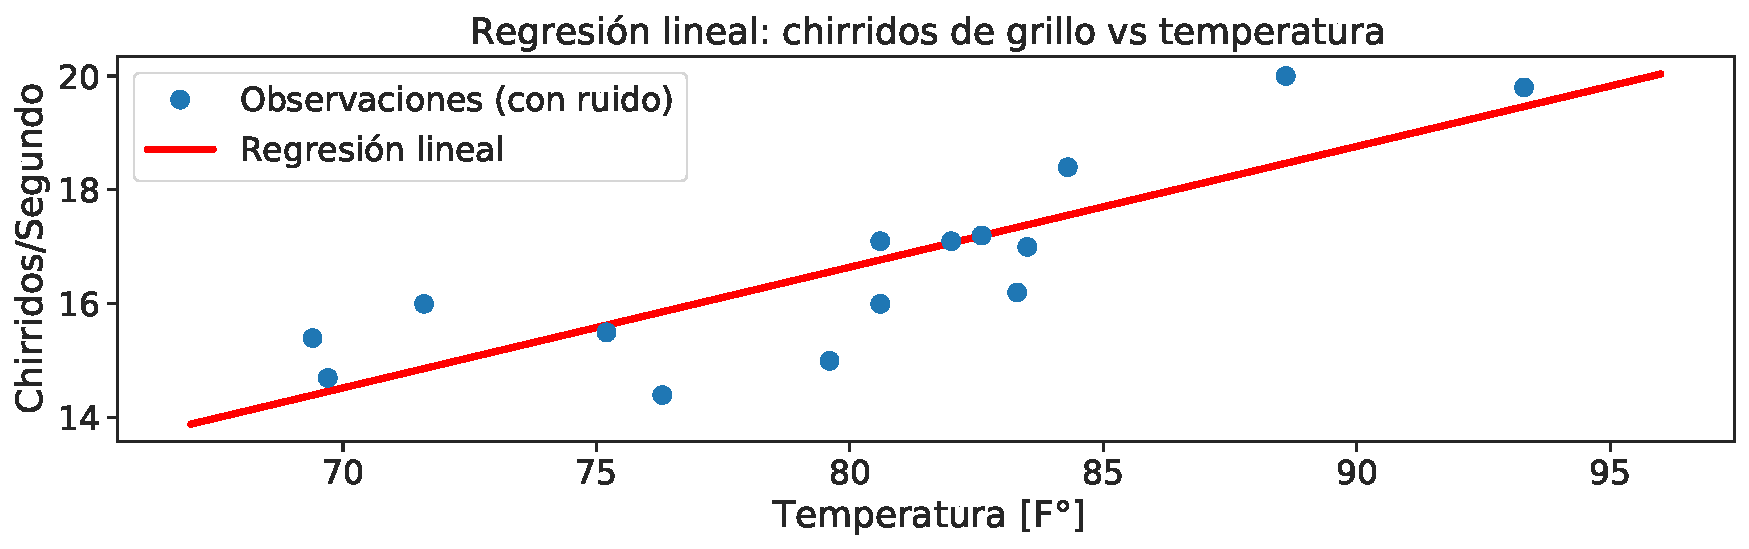
\includegraphics[width=0.9\textwidth]{img/cap1_chirridos.pdf}\\
	\caption{Ejemplo de regresión lineal usando mínimos cuadrados sobre la base de datos de chirridos versus temperatura.}
	\label{fig:reg_lin_1}
\end{figure}

La expresión $\left(\tX^\top\tX \right)^{-1} \tX^\top$ en la ec.~\eqref{eq:sol_mse} es conocida como\marginnote{Pseudo-inversa de Moore-Penrose}[-10pt] la pseudo-inversa de Moore-Penrose \cite[p.~7]{benisrael_greville_2006}. Observemos que una\marginnote{Condición necesaria para que este bien def.} condición \textbf{necesaria} para que esta pseudo-inversa esté bien definida es que la cantidad de observaciones ($N$) sea mayor o igual que la cantidad de dimensiones ($M+1$). Esto es porque la matriz $\tX^\top\tX$ es de tamaño $(M+1)\times(M+1)$ y su rango es $\min \{N, M+1\}$, consecuentemente, para que $\tX^\top\tX$ tenga rango completo (y por ende sea invertible), se debe cumplir al menos que $N\geq M+1$. Adicionalmente, una\marginnote{Condición necesaria y suficiente para la exist.} condición \textbf{necesaria y suficiente}  para la existencia de la solución de mínimos cuadrados en la ec.~\eqref{eq:sol_mse}, requiere que las $N\geq M+1$ observaciones\footnote{Recordemos que nos referimos a las observaciones aumentadas $\tilde{x}$} sean linealmente independientes, pues de esta forma los términos que componen la pseudo-inversa son efectivamente linealmente independientes y ésta tiene rango completo. Es claro que para el caso de variables continuas es muy poco usual que dos observaciones sean perfectamente colineales, sin embargo, en el caso de variables categóricas donde las observaciones son asignadas a un número finito de símbolos es probable que dos o más valores para la variable dependiente sean exactamente iguales. 

En la práctica, generalmente tendremos más observaciones que parámetros al considerar un modelo lineal y éstas serán linealmente independientes. Sin embargo, es posible que las observaciones sean tal que la inversión de la matriz  $\tX^\top\tX$ sea numéricamente  inestable. Esto ocurre fundamentalmente en dos casos ilustrados en el siguiente recuadro.  

\begin{mdframed}[style=discusion, frametitle={\center ¿Matriz cuasi-singular o incorrectamente escalada?}]

Al\marginnote{Matrices Cuasi-singulares} tratar de invertir una matriz de forma computacional, probablemente hemos obtenido un mensaje de la forma \texttt{matrix is singular, close to singular or badly scaled}. Veremos dos ejemplos para entender de dónde viene esta advertencia. 

\noindent\textbf{Caso 1:} Consideremos la matriz 
\begin{equation}
	A = \left[ \begin{matrix}10^{50} & 1 \\  10^{50}  & 2\end{matrix}\right]
\end{equation}
dicha matriz es claramente invertible y su inversa puede ser calculada mediante
\begin{equation}
	A^{-1} = \frac{1}{10^{50} \cdot 2 - 10^{50}\cdot 1}\left[ \begin{matrix}2 & -1 \\  -10^{50}  & 10^{50}\end{matrix}\right]
	=\left[ \begin{matrix}2\cdot10^{-50} & -10^{-50} \\  -1  & 1\end{matrix}\right],
\end{equation}
donde cuyos elementos difieren en 50 órdenes de magnitud. Sin embargo, la representación usual que consideramos cuando programamos es la de punto flotante de precisión simple, la cual considera el menor valor (de magnitud mayor que cero) de $2^{-127}\approx 10^{-38}$. Consecuentemente, los valores más pequeños que este límite serán aproximados por el elemento más cercano, es decir, cero. Utilizando la inversa aproximada, denotada $\tilde{A}^{-1}$, resulta en errores como el siguiente:
\begin{equation}
	A\tilde{A}^{-1} = \left[ \begin{matrix}10^{50} & 1 \\  10^{50}  & 2\end{matrix}\right] \left[ \begin{matrix} 0 & 0 \\  -1  & 1\end{matrix}\right] = \left[ \begin{matrix} -1 & 1 \\  -2  & 2\end{matrix}\right]
\end{equation}

\noindent\textbf{Caso 2:} Consideremos
\begin{equation}
	A = \left[ \begin{matrix} a  & a \\  b  & b + \epsilon\end{matrix}\right]
\end{equation}
la cual también es invertible para $a,\epsilon>0$, pues su determinante está dado por
\begin{equation}
	\det{A} = a(b+\epsilon) - ab = a\epsilon>0,
\end{equation}
sin embargo, si $\epsilon\ll1$ entonces el cálculo de la inversa puede sufrir inestabilidades numéricas como en el caso anterior. Sin embargo, observe para un $\eta>0$ suficientemente grande, la matriz $A+\eta I$ puede tener un determinante arbitrariamente grande (ver Sección \ref{sub:min_cuad_reg}).
\end{mdframed}

Es relevante reflexionar\marginnote{¿Por qué considerar MC como métr. de error?} por qué consideramos mínimos cuadrados como la métrica de error relacionada al problema de regresión. Existen varias razones por que lo hacemos, tanto técnicas como conceptuales, como también diversas desventajas de este criterio que es importante identificar.  Desde del punto de vista técnico, el costo convexo de un modelo lineal (en los parámetros) define un problema de optimización que también es convexo y por ende tiene una solución única. Además, en el caso particular del costo cuadrático, este óptimo puede ser determinado de forma explícita (lo cual es fuertemente deseado), pues está dado únicamente por la inversión de una matriz y no mediante, e.g., una búsqueda iterativa.

Desde un punto de vista conceptual, otra justificación para usar\marginnote{La med. del EC repres. la varianza muestral} la medida del error cuadrático es que éste representa la varianza muestral. Es decir, si considerásemos que $x_i$ e $y_i$ son observaciones iid de variables aleatorias (VAs) $x$ e $y$ respectivamente, entonces el error cuadrático (relacionado con la función $f$) definido por
\begin{equation}
	e= \sum_{i=1}^N (y_i-f(x_i))^2,
\end{equation}
es la varianza muestral de la variable aleatoria $y-f(x)$, definida como el \emph{error} de estimación. De igual forma, la varianza de la suma de múltiples variables aleatorias (pensemos en errores acumulados, los cuales son independientes) corresponde a la suma de las varianzas de dichas VAs. Esto ocurre precisamente cuando usamos el exponente igual a 2, y no si usáramos 1.95 o 2.05. 

Podemos además justificar el\marginnote{Motivación geométrica para ocupar el EC} uso del error cuadrático con una motivación geométrica. Recordemos que el problema de regresión (lineal) requiere encontrar una solución aproximada de un sistema lineal sobredeterminado definido por 
\begin{equation}
	\tX \theta = Y,\label{eq:sist_lineal_sobredet}
\end{equation}
donde la cantidad de incógnitas ($M+1$) es ampliamente superada por el número de ecuaciones ($N$). Como esta solución, desde el punto de vista de un sistema lineal, no existe, uno puede proceder a encontrar la solución para $\theta$ que reporta \emph{la menor discrepancia} entre ambos lados de la ec.~\eqref{eq:sist_lineal_sobredet}. En este sentido, podemos identificar el espacio formado por todos los posibles valores que toma la combinación lineal $\tX \theta$ para distintos valores de $\theta\in\R^{M+1}$, es decir, el \emph{span} de todas las columnas de $\tX$ (los datos) definido como el \emph{espacio de las columnas de} $\tX$ o, simplemente, $\text{span}(\tX)$. Luego, podemos identificar el elemento de dicho espacio que está más cerca de $Y$  como la proyección del propio $Y$ en $\text{span}(\tX)$. Esto está ilustrado en la Fig.~\ref{fig:projection}, donde la condición para identificar dicha proyección es  precisamente que el vector error $\tX \theta- Y$ sea ortogonal al espacio  $\text{span}(\tX)$ generado por los datos (de entrada), consecuentemente, ocupando el producto interno tenemos que 
\begin{equation}
	(\tX \theta- Y)^\top \tX = 0,
\end{equation}
lo cual nos lleva directamente a la solución de mínimos cuadrados. 

\begin{figure}[t]
	\centering
	\includegraphics[width=0.5\textwidth]{img/LinRegGeo.pdf}\\
	\caption{Interpretación geométrica de la regresión lineal y mínimos cuadrados}
	\label{fig:projection}
\end{figure}

Finalmente, notemos que el\marginnote{Desv. del criterio de MC} criterio de  mínimos cuadrados (MC) también tiene desventajas. Implícitamente, MC está intrínsecamente relacionado con un supuesto de gaussianidad de los datos---esto será evidente cuando estudiemos el criterio de máxima verosimilitud---consecuentemente, el uso de MC produce estimaciones razonables cuando la relación entre $x$  e $y$ es simétrica y sin \emph{grandes desviaciones}. Por el contrario, cuando existen datos  que se alejan mucho de dicha la tendencia buscada, las estimaciones encontradas mediante MC pueden desviarse considerablemente de la solución buscada, esto se debe precisamente a la contribución cuadrática del error, donde, coloquialmente, una muestra \emph{muy alejada} pesa tanto o más que varias muestras \emph{ligeramente alejadas}. La Fig.~\ref{fig:reg_lin_2} ilustra este fenómeno para el mismo ejemplo de los chirridos en la Fig.~\ref{fig:reg_lin_1}, donde se ha introducido un \emph{outlier}, es decir, una observación que está inusualmente alejada de los datos y se ha recalculado el resultado de la regresión lineal mediante el criterio de MC. Se puede ver cómo se deteriora la estimación solo con la introducción de un nuevo dato. 



\begin{figure}[H]
	\centering
	\includegraphics[width=0.9\textwidth]{img/cap1_chirridos_outlier.pdf}\\
	\caption{Efecto de un \emph{outlier} en la regresión lineal usando mínimos cuadrados: Se ha agregado un dato erróneo (\emph{outlier} en gris) y se ha recalculado la regresión lineal, note cómo la inclusión de dicho punto deteriora el resultado de la regresión.}
	\label{fig:reg_lin_2}
\end{figure}

La\marginnote{Elección de una métrica \textit{ad hoc} al problema} lección que queda de este ejemplo es que debemos considerar una métrica \emph{ad hoc} al problema que estamos considerando, por ejemplo, si es muy probable que existan outliers, no debemos penalizar cuadráticamente los errores. De igual forma, al elegir una métrica de error debemos verificar cuán relevante es que el error de regresión sea i) nulo vs muy pequeño, o bien ii) grande vs extremadamente grande. La Fig.~\ref{fig:reg_lin_err} presenta cuatro métricas de error (como función del propio error), donde podemos interpretar sus propiedades. 

\begin{figure}[H]
	\centering
	\includegraphics[width=0.8\textwidth]{img/cap1_errores.pdf}\\
	\caption{Distintas funciones de costo en función del error de estimación, de izquierda a derecha: cuadrático, absoluto (crecimiento lineal en función del error), $\epsilon$-insensible (es irrelevante si el error está entre 0 o  $\epsilon$) y acotado (es irrelevante si el error es mayor que cierto umbral).}
	\label{fig:reg_lin_err}  
\end{figure}


\subsubsection{Regularización: ajuste versus generalización} % (fold)
\label{sub:min_cuad_reg}

Perseguir ciegamente la solución de mínimos cuadrados puede resultar, como discutimos en la sección anterior, en situaciones donde la inversa de Moore-Penrose sea \emph{cercana} a singular, especialmente en los casos que las observaciones son parecidas o redundantes. En este sentido, debemos considerar un criterio que no simplemente busque un ajuste a los datos, sino que también promueva ciertas propiedades de la solución, por ejemplo, suavidad, bajas magnitudes de los parámetros o incluso pocos parámetros. Nos referiremos a estas soluciones como \emph{regulares}, y el objetivo de esttet apartado será \emph{regularizar} la solución de mínimos cuadrados.

Las penalizaciones a considerar en el problema de regresión pueden ser codificadas directamente en la función de costo. Por ejemplo, ésta puede incluir un término que promueve el ajuste de los datos y otro término que sanciona soluciones que se alejan de lo deseado. Un criterio estándar de penalización es el basado en la norma de los parámetros, es decir, 
\begin{equation}
	J_\rho = \frac{1}{2}\sum_{i=1}^N(y_i-\theta^
	\top \tx_i)^2 + \frac{\rho}{p}||\theta||_p^p,\ p\in\R_+,
	\label{eq:reg_least_squares}
\end{equation} 
donde $||\cdot||_p$ denota la norma $\ell_p$, es decir, $||\theta||_p=\left(\sum_{j=1}^N|\theta_j|^p\right)^\frac{1}{p}$ y el parámetro $\rho\geq0$ tiene el rol de balancear la importancia entre ajuste (primer término) y regularidad de la solución (segundo término). Distintos valores de $p$ inducen distintos propiedades sobre las soluciones, siendo las más usadas las correspondientes a $p=1$, conocido como \textbf{LASSO}\footnote{\emph{Least Absolute Shrinkage and Selection Operator.}} \cite{tibshirani_1996}, y $p=2$ conocido como \textbf{regularización de Tikhonov} \cite{tikhonov_arsenin_1977} o bien \textbf{\emph{Ridge Regression}} \cite{hoerl_kennard_1970}.  

Una ventaja de la regularización de Tikhonov es que su solución, al igual que el caso de mínimos cuadrados no regularizados, puede ser encontrada en forma exacta. En efecto, para $p=2$ el término de regularización puede ser expresado como $||\theta||_2 = \theta^\top\theta$, con lo que el minimizante del costo cuadrático regularizado está dado por: 
\begin{align}
\nabla_\theta J_\rho=0 &\Leftrightarrow \sum_{i=1}^N(\theta^\top \tx_i - y_i)\tx_i^\top + \rho\theta^\top=0  							&&\text{def. $J$}\nonumber\\  
&\Leftrightarrow \sum_{i=1}^Ny_i\tx_i^\top = \sum_{i=1}^N\theta^\top \tx_i\tx_i^\top + \rho\theta^\top					&&\text{ordenar}\nonumber\\
&\Leftrightarrow \theta^\top = \sum_{i=1}^Ny_i\tx_i^\top \left(\sum_{i=1}^N \tx_i\tx_i^\top + \rho \eye\right)^{-1}	&&\text{despejar $\theta^\top$}\nonumber\\
&\Leftrightarrow \theta =  \left(\sum_{i=1}^N \tx_i\tx_i^\top +\rho \eye\right)^{-1} \sum_{i=1}^N \tx_i y_i 		&&\text{transponer}\nonumber\\
&\Leftrightarrow \theta = \left(\tX^\top\tX +\rho \eye\right)^{-1} \tX^\top Y.								&&\text{def. $\tX$ y $Y$} \label{eq:least_sq_soln}
\end{align}

De la última expresión, es posible ver que el requerimiento de que las observaciones disponibles sean (i) más que la dimensión $M+1$ y que además (ii) éstas sean colineales ya no es necesario para que la solución esté bien definida. De hecho, la matriz $\tX^\top\tX$ puede efectivamente estar cercana a ser no invertible, sin embargo, es posible \emph{regularizar} la solución forzando que la matriz $\left(\tX^\top\tX +\rho \eye\right)$ sea arbitrariamente lejana de las matrices singulares (o tenga un determinante arbitrariamente grande) aumentando el valor de $\rho$. 




Es relevante entender por qué una disminución en la norma de los parámetros, puede ayudar a ajustar \emph{mejores} modelos. A primera impresión, un podría pensar que el criterio de mínimos cuadrados regularizados (MCR) en ningún caso puede reportar mejores modelos que su contraparte MC, pues MCR es una variante restringida del problema original y consecuentemente solo puede \emph{en el mejor de los casos} alcanzar la solución óptima. Esto es cierto si por \emph{mejor modelo} solo consideramos el error cuadrático medio (ECM), sin embargo, solo enfocarse en esta métrica no siempre es el mejor opción. Para ilustrar este concepto, tomemos las siguientes consideraciones: asumamos que efectivamente los datos cumplen la relación
\begin{equation}
	y_i = \underbrace{\theta^\top\tx_i}_{f_i} + \epsilon_i,	
 \end{equation}
 donde $\epsilon_i$ son observaciones iid de una variable aleatoria de varianza $\sigma^2$, $\theta$ es un parámetro fijo, los $\tx_i$ son fijos y $f_i= \theta^\top\tx_i$ se refiere a la  \emph{parte determinista} del modelo. Además, consideremos una estimación del parámetro $\theta$ construida en base a un conjunto de entrenamiento $D=\{(\tx_i,y_i)\}_{i=1}^N$, denotada $\hat\theta=\hat\theta_D$. Con estas consideraciones, para un nuevo par $(\tx_\star,y_\star)$, podemos escribir el \emph{costo (cuadrático) esperado} asociado a la \textbf{predicción} $\hat f_\star = \hat\theta^\top \tx_\star$ mediante el \emph{trade-off} entre sesgo y la varianza \cite{ISLbook} dado por
\begin{equation}
 	\E{(y_\star - \hat f_\star)^2} = \text{Sesgo}(\hat f_\star)^2 + \text{Varianza}(\hat f_\star) + \sigma^2,\label{eq:expected_sq_loss}
 \end{equation} 
 donde el valor esperado es tomado con respecto a la ley de $\epsilon$, la única fuente de incertidumbre en este escenario, y 
 \begin{itemize}
 	\item $\text{Sesgo}(\hat f_\star) = \E(\hat f_\star) - f_\star$, es una medida de exactitud: ¿cuán buena (en valor esperado) es la estimación con respecto al valor real?
 	\item $\text{Varianza}(\hat f_\star)= \E(\E(\hat f_\star)- \hat f_\star)^2$, es una medida de precisión: ¿cuán disperso es el estimador?
 	\item $\sigma^2$ es es la varianza de \emph{ruido} $\epsilon$ y es la parte irreducible del costo, en el sentido que no puede ser controlada por la elección de $\hat\theta$.
 \end{itemize}

Podemos evaluar el sesgo y la varianza para el estimador de mínimos cuadrados, denotado $\hat\theta_{MC}$, eligiendo $\hat f_\star = \hat\theta_{MC}^\top\tx_\star$. En efecto,  
\begin{align}
	\text{Sesgo}(\hat f_\star) &= \E(\theta_{MC}^\top\tx_\star) - \theta^\top\tx_\star=0\\
	\text{Varianza}(\hat f_\star) &= \sigma^2 \tx_\star^\top (\tX^\top\tX)^{-1}	\tx_\star
\end{align}
Es decir, el modelo de regresión lineal ajustado mediante MC reporta un estimador insesgado (sesgo nulo) pero con una varianza que depende de los datos en el conjunto de entrenamiento $D$, la varianza del ruido $\sigma^2$ y la propia entrada $\tx_\star$. Si bien no es posible determinar cuánto es esta varianza sin tomar supuestos estadísticos sobre los $\tx_i$'s, recordemos que la matriz $\tX^\top\tX$ puede ser cercana a singular cuando los datos son pocos, redundantes o colineales, lo cual resultará en alta varianza para la predicción $\hat f_\star$. De hecho, si asumiéramos que $\tx_i\sim\cN(0,1)$ iid, tendríamos que $\text{Varianza}(\hat f_\star) = \sigma^2 M/N$, es decir, la varianza es inversamente proporcional a la razón entre la dimensión de las entradas ($M$) y la cantidad de muestras ($N$).

\begin{mdframed}[style=discusion, frametitle={\center Evaluaciones \emph{dentro de muestra} y \emph{fuera de muestra}}]
 Notemos que la expresión en la ec.~\eqref{eq:expected_sq_loss} es una medida de error \emph{fuera de muestra}, pues evalúa un estimador $\hat\theta$, construido en base a un conjunto $D$, en un nuevo dato $(\tx_\star,y_\star)$ que no está originalmente contenido en $D$. No debemos confundir esta expresión con el error cuadrático medio, en la ec.~\eqref{eq:least_squares_cost}, el cual representa un error \emph{dentro de muestra}. La  evaluación de ambos tipos de  costos es clave para diseñar modelos y estimadores que puedan \emph{generalizar} a datos no vistos. 
\end{mdframed}

Al penalizar la norma cuadrada del parámetro $\theta$, la regresión de Ridge sacrifica la propiedad insesgada del estimador, pero en retorno construye un estimador que tiene menos varianza que el de MC. Esto puede entenderse como el balance entre: i) confiar únicamente en los datos, los cuales pueden ser pocos o muy ruidoso y consecuentemente insuficientes para determinar un modelo apropiado, y ii) introducir un \emph{sesgo} al modelo (por ejemplo, parámetros pequeños) con la finalidad de robustecer el modelo encontrado en función de los datos disponibles. Esta noción de (sobre-)ajustar a los datos de entrenamiento versus generalizar a  nuevos  puede ser ilustrada con el siguiente ejemplo: Consideremos $N=1000$ datos relacionados linealmente (pares de entrada y salida) donde la dimensión de entrada es $M=100$ generados por el siguiente script.
\begin{lstlisting}[language=Python]
##generacion de datos relacionados linealmente 
n_samples, n_features = 1000, 100
rng = np.random.RandomState(0)
X = rng.randn(n_samples, n_features)
theta = rng.randn(n_features,1)
y = X@theta + 10*rng.randn(n_samples, 1)
\end{lstlisting}
 En vez de utilizar todas las muestras de entrenamiento, utilicemos solo $N'=15$ muestras para entrenar usando los criterios de MC, y regresión de Ridge (RR) con $\rho\in\{40,80\}$. Repitiendo este proceso 400 veces, podemos analizar cómo se comportan los distintos métodos en cuanto a la magnitud de los parámetros encontrados, el error dentro de muestra (con respecto a los datos de entrenamiento) y el error fuera de muestra (con respecto a los datos no usados para entrenar). La Fig.~\ref{fig:MCvsRR_Synth} muestra dichos histogramas, desde donde podemos ver que a mayor $\rho$ (recordemos que MC es equivalente a RR con $\rho=0$), los parámetros encontrados tienen menor magnitud. Adicionalmente, notemos que el modelo no regularizado (MC) se comporta mejor en evaluación dentro de muestra, sin embargo, sus papeles se invierten cuando se trata de evaluación fuera de muestra: el incluir un sesgo en el ajuste de modelos (RR) puede ayudar a generalizar y no sobreajustar cuando se tienen pocos datos. 

 \begin{figure}[H]
	\centering
	\includegraphics[width=0.8\textwidth]{img/cap1_bias-variance.pdf}\\
	\caption{Mínimos cuadrados versus regresión de Ridge ($\rho\in\{40,80\}$): determinación de parámetros usando solo 15 muestras para un parámetro de dimensión $M=100$. De derecha a izquierda podemos ver magnitud de los parámetros encontrados, error dentro de muestra y error fuera de muestra. Experimento repetido 400 veces.}
	\label{fig:MCvsRR_Synth}  
\end{figure}



\subsubsection{Formulación con restricciones y selección de variables} % (fold)
\label{sub:restricciones}

Para ilustrar cómo el proceso de regularización es equivalente a restringir los parámetros a cumplir con una condición específica, e.g., tener una magnitud dada, consideremos el siguiente problema de regresión lineal con restricciones:
\begin{align}
	\min_\theta &\frac{1}{2}\sum_{i=1}^N (y_i-\theta^\top\tx_i)^2\label{eq:MC_restriccion}\\
	\text{s.a.} &\ ||\theta||_p^p = \tau,\nonumber
\end{align}
donde asumiremos que $\tau\geq0$ es una constante conocida. Sabemos que este problema puede ser resuelto en su forma dual mediante la formulación del Lagrangiano dado por 
\begin{equation}
	L = \frac{1}{2}\sum_{i=1}^N (y_i-\theta^\top\tx_i)^2 - \lambda (||\theta||_p^p - \tau),
\end{equation}
donde $\lambda\geq0$ es conocido como el \emph{multiplicador de Lagrange}. Luego, las condiciones de primer orden necesarias para encontrar la solución del problema con restricciones en la ec.~\eqref{eq:MC_restriccion} están dadas por: 
\begin{align}
	\frac{\partial L}{\partial \theta} = 0 &\quad\Rightarrow\quad  \frac{\partial }{\partial \theta}\left( \frac{1}{2}\sum_{i=1}^N (y_i-\theta^\top\tx_i)^2 - \lambda ||\theta||_p^p \right) = 0\label{eq:dual_MCR1}\\
	\frac{\partial L}{\partial \lambda} = 0 &\quad\Rightarrow\quad ||\theta||_p^p = \tau, \label{eq:dual_MCR2}
\end{align}
lo cual recupera la forma del problema de minimización de mínimos cuadrados regularizados. Enfatizamos esta relación en el siguiente recuadro. 


\begin{mdframed}[style=discusion, frametitle={\center Mínimos cuadrados regularizados: optimización con restricciones}]
Observemos que el problema de mínimos cuadrados regularizados, determinado por el costo en la ec.~\eqref{eq:reg_least_squares}, es equivalente al dual de un problema de optimización con restricciones en las ecs.~\eqref{eq:dual_MCR1}-\eqref{eq:dual_MCR2} para un $\lambda$ dado tal que $\lambda =-{\rho}/{p}$. Consecuentemente, como el valor óptimo de $\lambda$ depende del nivel de la restricción $\tau$, podemos aseverar que \textbf{para cualquier $\rho\geq0$, existe un $\tau\geq0$ tal que la minimización de \eqref{eq:reg_least_squares} es equivalente a la de \eqref{eq:MC_restriccion}.} Consecuentemente,  podemos interpretar el problema de MCR como el de MC sujeto a una restricción para (en este caso la norma) del parámetro. 
	
\end{mdframed}

Con la interpretación del problema de optimización con restricciones sobre la norma del parámetro $\theta$, podemos entender distintos regularizadores (distintos $p\geq0$) mediante sus curvas de nivel. La Fig.~\ref{fig:reg_lin_reg} ilustra las curvas correspondientes al costo cuadrático (izquierda) y al término de regularización en la eq.~\eqref{eq:reg_least_squares} para órdenes $p\in\{0.5,1,2\}$. 

\begin{figure}[H]
	\centering
	\includegraphics[width=0.8\textwidth]{img/cap1_regularizadores.pdf}\\
	\caption{Curvas de nivel del costo cuadrático para un problema hipotético con solución $\theta=[10,20]$ (izquierda) y términos de regularización para órdenes $p\in\{0.5,1,2\}$. Observe cómo las curvas de nivel atraen el mínimo hacia el origen de distinta forma: $p=2$ lleva la solución directamente al origen, mientras que $p\in\{0.5,1\}$ lleva la solución a los bordes, es  decir, privilegiando soluciones ralas. La solución $\theta=[10,20]$ se ha denotado con una cruz azul, recuerde que solo el costo cuadrático depende de este valor, no los términos de regularización. }
	\label{fig:reg_lin_reg}  
\end{figure}

La formulación en base a restricciones es clave para entender la propiedad de \emph{selección de características} de los MCR. Al estimar el parámetro $\theta$, estamos verificando cuán importante es cada (coordenada de la) entrada o en la jerga de reconocimiento de patrones, cada \emph{característica}. Indirectamente estamos también implícitamente descubriendo cuáles son las características que importan y cuales no, a esto nos referimos como selección de características. Distintas normas para el término de regularización, como las ilustradas en la Fig.~\ref{fig:reg_lin_reg}, inducen distintas propiedades para la solución del problema de MCR. En particular, RR atrae \emph{homogéneamente} el parámetro hacia el origen, lo cual resulta  en estimaciones de menor varianza como vimos en el apartado anterior. LASSO ($p=1$) y el caso $p\leq1$ en general presenta una propiedad adicional, donde la forma de la curva de nivel permite que usualmente la solución del problema se concentre el las puntas del \emph{diamante} (ver Fig.~\ref{fig:reg_lin_reg}, $p=1$), llevando algunas coordenadas del parámetro $\theta$ directamente a cero. Por esto decimos que LASSO (y $p\leq1$ en general) tiene la propiedad de selección de variables y entrega modelos ralos con respecto a MC tradicional. 

Para ilustrar la propiedad de selección de características, consideremos el \emph{Breast Cancer Wisconsin Data Set}\footnote{\url{https://archive.ics.uci.edu/ml/datasets/breast+cancer+wisconsin+(original)}}, el cual tiene $N=569$ muestras y un dimensión de entrada de $M=30$. Los valores para la variable de salida ($y$) son solo dos, pues este es un problema de clasificación (\emph{cáncer} vs \emph{no-cáncer}), sin embargo, nosotros ajustaremos un modelo de regresión lineal usando MC, RR y LASSO para luego evaluar los pesos encontrados. Usaremos 2/3 de los datos para entrenar y el 1/3 restante para calcular puntajes fuera de muestra. La Fig.~\ref{fig:MC_RR_LASSO_breastcancer} presenta los parámetros encontrados para cada uno de los métodos, donde podemos ver la propiedad de selección de variables de LASSO; adicionalmente, la Tabla \ref{tab:breastMC_RR_LASSO} muestra los puntajes de cada método, tanto dentro como fuera de muestras: en la línea de la discusión anterior, los modelos regularizados presentan mejor generalización y usan menos parámetros (o más parámetros iguales a cero). 


\begin{table}
\centering
\caption{Puntajes de modelos de regresión implementados en \emph{Breast Cancer Wisconsin Data Set}, más alto es mejor. Observe la superioridad de los modelos regularizados para generalizar.}
	\label{tab:breastMC_RR_LASSO}
	\begin{tabular}{ r|c|c } 
		 & in-sample & out-of-sample \\
		\hline
		MC & \textbf{0.7896} & 0.6911 \\ 
		RR & 0.6905 & 0.6903 \\ 
		LASSO & 0.7452 & \textbf{0.7242}
	\end{tabular}
\end{table}



 



\begin{figure}[H]
	\centering
	\includegraphics[width=0.8\textwidth]{img/cap1_OLS_RR_LASSO.pdf}\\
	\caption{Parámetros de la regresión lineal del \emph{Breast Cancer Dataset} usando MC, RR y LASSO. Observe cómo RR y LASSO disminuye críticamente la magnitud de los parámetros y, además, LASSO lleva parámetros directamente a cero, resultando en un modelo más simple (i.e, con menos parámetros).}
	\label{fig:MC_RR_LASSO_breastcancer}  
\end{figure}



\begin{mdframed}[style=discusion, frametitle={\center Regularización: Consideraciones generales}]
Para concluir esta sección, enunciamos las siguientes preguntas para discusión posterior\\
$\bullet$ \textbf{¿es justo comprar MC y MCR en términos del ECM?} Ciertamente no, el criterio de MC siempre reportará un menor ECM, pues ha sido entrenado para minimizar dicho costo. Las ventajas de MCR están en su desempeño fuera de muestra, selección de variables o en  general en su habilidad de  incorporar  sesgo  \emph{de diseñador} en la soluciones que no afloren naturalmente de  los  datos. \\
$\bullet$ \textbf{¿cómo elegir $\rho$?} De forma general, este \emph{hiperparámetro} determina el balance entre regularización (cuán  sesgado) y ajuste (cuán bien replica  los datos ), consecuentemente lo debemos elegir según nuestra intención. En la práctica,  podemos evaluar el desempeño de distintos valores de $\rho$ fuera de muestra con la finalidad de elegir un valor apropiado. Esta técnica se llama \emph{validación cruzada} y busca determinar modelos que no sufran de subajuste, o sobreajuste.\\
$\bullet$ Vimos que la norma $\ell_p$ con $0<p\leq1$ tiene la propiedad de selección de características, pero, \textbf{¿qué pasa con la `norma' $\ell_0$?}. La cantidad  $\ell_0(\theta)$ denota la cantidad de elementos no nulos de $\theta$ y no es una norma, sin embargo, puede de todas formas ser usada en la definición del costo en la ecu.~\eqref{eq:reg_least_squares}, con la finalidad de directamente penalizar la cantidad de características usadas por el modelo. Desafortunadamente, encontrar la solución usando la ``norma'' $l_0$ es muy difícil, sin embargo, bajo ciertas condiciones la consideración de la norma $l_1$ puede llevar a la misma solución.
\end{mdframed}

\subsection{Máxima verosimilitud} % (fold)
\label{ssub:max_ver}


En el apartado anterior vimos que el criterio de  mínimos cuadrados, y su variante regularizada, ofrecen una alternativa simple, elegante, interpretable y con solución en forma cerrada. Sin embargo, también vimos que dicho criterio sufre de desventajas en cuanto a su capacidad de ajustar modelos en casos generales, pues el criterio de MC es particularmente apropiado para variables contínuas, con perturbaciones aditivas  y simétricamente dispersas con respecto a una tendencia dada. Existen distintos casos donde el criterio de MC no es apropiado, por ejemplo aplicaciones financieras con  perturbaciones multiplicativas, mediciones de intensidad como frecuencia de aparición de palabras o sismos en donde las perturbaciones son con alta probabilidad solo positivas, y problemas de clasificación o asignación (\emph{clustering}) en donde las métricas de error toman la forma como ``correcto''/``incorrecto'', con lo que una medida de error que que reporte ajustes ``más incorrectos'' no tiene sentido. 

Una alternativa natural es considerar una métrica de desempeño distinta y diseñada específicamente en función  de cada aplicación con la finalidad de capturar asimetrías, no-estacionariedad, asignación correcta e invarianzas (en el problema de \emph{clustering} por ejemplo) entre otras propiedades. Sin embargo, esta no solo es una tarea tediosa y poco elegante---en el sentido que va en contra los objetivos de inteligencia artificial expuestos en el Capítulo~\ref{cap:intro}---sino que puede ser muchas veces impracticable, pues precisamente no conocemos cuáles son las propiedades de los datos antes de ajustar modelos. Además, usar distintas métricas dificulta la interpretación y comparación de los enfoques considerados. Consecuentemente, nos proponemos considerar un criterio global de ajuste de modelos, el que en cada caso particular \emph{colapse} a una forma explícita que sí es \emph{ad hoc} al problema/modelo en cuestión y permite comparar distintos enfoques de manera unificada. 	

El enfoque general para ajuste de modelos que consideraremos en esta sección, y continuaremos utilizando durante el resto del curso, será el \emph{criterio  de máxima verosimilitud}, dado un conjunto de datos de entrenamiento $D$. Este es un criterio general para una amplia gama de modelos el que, tal como se mencionó en el párrafo anterior, toma una  forma específica en cada problema, aunque su solución no siempre es calculable de forma explícita. Este enfoque es radicalmente distinto al de MC y a cualquier otro criterio de ``ajuste'': con el criterio de MC buscamos un modelo \emph{aproximado} a los datos, donde sabemos que ningún modelo es el modelo correcto, tal que la discrepancia entre el modelo candidato ya los datos sea mínima. Por el contrario, en el criterio de \emph{máxima verosimilitud} nuestro objetivo es encontrar el modelo que---con mayor probabilidad---ha generado \emph{exactamente} los datos observados. Debido a la naturaleza aleatoria de los datos, para implementar este concepto es necesario considerar modelos probabilísticos, de forma de poder calcular la probabilidad de que los datos $D$ hayan sido generados por un modelo $m$, luego, elegiremos  el modelo que maximice dicha probabilidad. 

El criterio de máxima verosimilitud (MV) es aplicable a modelos probabilísticos para la generación de datos, a los cuales nos referiremos como \emph{modelo generativos}. Para el caso del problema de regresión, el modelo generativo es cualquiera que modele la variable de salida como una variable aleatoria $y$ a través de una distribución condicional (a la entrada $x$ y el parámetro $\theta$) de la forma 
\begin{equation}
	y|x,\theta \sim p(y|x,\theta),\label{eq:mod_gen}
\end{equation}
donde enfatizamos que $y$ es  la única variable aleatoria y tanto el parámetro $\theta$ como la entrada $x$ son cantidades fijas (la primera desconocida y la segunda conocida).

\begin{mdframed}[style=discusion, frametitle={\center Notación sobre variables aleatorias}]
 Estrictamente, en base a la notación estándar en probabilidades, la expresión  correcta para el lado izquierdo de la ec.~\eqref{eq:mod_gen} debiese ser  
 \begin{equation}
  	Y=y|x,\theta,
  \end{equation}
  pues $Y$ denota la variable aleatoria, e $y$ el valor que ésta toma. Sin embargo, seguiremos la usanza de la comunidad de Aprendizaje de Máquinas donde denotamos la tanto la variable aleatoria como su valor indistintamente con la letra minúscula, e.g., $y$. Seguiremos esta notación a menos que sea estrictamente necesario para evitar confusión. Además, en todos los casos asumiremos que las distribuciones de probabilidad consideradas tienen densidad con respecto a alguna medida---usualmente \emph{Lebesgue} (caso continuo) o \emph{cuenta-puntos} (caso discreto)---ambas denotadas indistintamente por $p(\cdot)$.  Finalmente, usualmente escribiremos 
  \begin{equation}
  	y|x \sim p(y|x),
  \end{equation}
  sin enunciar explícitamente la dependencia del parámetro $\theta$.
\end{mdframed}


En particular, en el caso de la regresión lineal podemos considerar el siguiente modelo  generativo:
\begin{equation}
	y = a^\top x + b + \epsilon,\quad \epsilon\sim\cN(0,\sigma_\epsilon^2),
	\label{eq:lin_gauss}
\end{equation}
el cual consta de una parte determinística (lineal en $x$) y una parte aleatoria caracterizada por la variable aleatoria $\epsilon$, la cual hemos  elegido gaussiana con media cero y varianza $\sigma_\epsilon^2$. El modelo probabilístico en la ec.~\eqref{eq:lin_gauss} puede expresarse en mediante la siguiente densidad condicional 
\begin{equation}
	y|x \sim p(y|x,\theta) = \cN(y;a^\top x + b ,\sigma_\epsilon^2),\label{eq:mod_lin_gau}
\end{equation}
donde hemos denotados el vector de todos los parámetros del modelo mediante $\theta = [a,b,\sigma_\epsilon^2]$.

Si bien, lo siguiente no es necesario en el caso general, usualmente asumiremos que las realizaciones del modelo anterior, i.e., los datos $\{y_i\}_{i=1}^N$ generados a partir de la entrada $\{x_i\}_{i=1}^N$, son \textbf{condicionalmente independientes} dado el modelo. Esto significa que \emph{si conociésemos el modelo}, o  equivalentemente, si conociésemos $\theta$, y dos entradas $x_i,x_j$, entonces las  salidas correspondientes $y_i,y_j$ son independientes. Es importante clarificar que los valores generados por el modelo $\{y_i\}_{i=1}^N$ \textbf{no son independientes}. En efecto, si fuesen independientes no podríamos hacer predicciones: la predicción de una observación nueva $y_\star$ en base a una secuencia de observaciones $\{y_i\}_{i=1}^N$ estaría dada por\footnote{Hemos ignorado la dependencia de las variables independientes $\{x_i\}_{i=1}^N$, $x_\star$.}
\begin{equation}
	\blueb{[esto es falso]}\qquad p(y_\star|\{y_i\}_{i=1}^N) 
	\stackrel{\text{(prob. cond.)}}{=} \frac{p(y_\star,\{y_i\}_{i=1}^N)} {p(\{y_i\}_{i=1}^N)} 
	\stackrel{\text{(indep.)}}{=} \frac{p(y_\star),p(\{y_i\}_{i=1}^N)} {p(\{y_i\}_{i=1}^N)}
	=p(y_\star), 
\end{equation}
es decir, las observaciones pasadas no aportarían para la predicción.  Por  el contrario, como nuestro supuesto es de \textbf{independencia condicional} la expresión correcta es  la siguiente: 
\begin{equation}
	\blueb{[esto es verdadero]} \qquad p(y_\star|\{y_i\}_{i=1}^N,\theta)  
	=p(y_\star|,\theta), \qquad  \qquad\qquad  \qquad \qquad  \qquad\qquad  \qquad
\end{equation}
lo cual quiere decir que las  observaciones pasadas no son útiles para predecir el  futuro \textbf{solo si conozco el modelo}. Esto es evidente, pues si conozco el modelo, no necesito datos para saber de $y_\star$. 


El supuesto de independencia condicional está garantizado al imponer que las realizaciones de $\epsilon\sim\cN(0,\sigma_\epsilon^2)$ sean \emph{independientes e idénticamente distribuidas} (iid). Esto es  fundamental para poder aprender el modelo desde múltiples observaciones, pues intuitivamente todas las observaciones aportan evidencia no redundante sobre el parámetro en común $\theta$. Por el contrario, si las observaciones fuesen condicionalmente dependientes, entonces la información que reportan para estimar $\theta$ sería redundante. Igualmente, si no todas las observaciones siguiesen la misma distribución, entonces cada una tendría ``su propio $\theta$'' y solo tendríamos ``un  dato'' para estimar cada parámetro. Más adelante en el curso veremos casos donde los datos no son iid pero asumimos cierta regularidad en los modelos que permiten determinar sus parámetros.  

\subsubsection{Función de verosimilitud} % (fold)
\label{sssub:verosimilitud} 

\begin{definition}[Verosimilitud]
Consideremos un  modelo generativo definido mediante la densidad de  probabilidad  $y\sim p(y|\theta)$, donde el  parámetro $\theta\in\Theta$ y un conjunto de observaciones $\{y_i\}_{i=1}^N$ generado por dicho modelo. La función $L(\theta): \Theta \to \R$ definida como la probabilidad de los datos observados condicional al parámetro $\theta$, es decir, 
\begin{equation}
			\theta   \mapsto L(\theta) =  p(\{y_i\}_{i=1}^N | \theta),
\end{equation}
es conocida como \emph{verosimilitud} del modelo $p(y|\theta)$ o, equivalentemente, del  parámetro $\theta$. En algunos casos, consideraremos la  notación $L_\y(\theta)$ para enfatizar que la verosimilitud es tomada con respecto a las observaciones  $\y$.
\end{definition}

La definición anterior es elocuente: la función de verosimilitud precisamente cuantifica cuán verosímil es un modelo (o equivalentemente, parámetro) de haber generados las observaciones $\{y_i\}_{i=1}^N$. En este sentido, ante dos valores candidatos para el parámetro, por ejemplo $\theta_1$ y $\theta_2$, éstos pueden se evaluados mediante la comparación de $L(\theta_1)$ y $L(\theta_2)$, en efecto, si la razón $L(\theta_1)/L(\theta_2)$ es, por ejemplo, 3, entonces diremos que \emph{el valor de $\theta$ sea $\theta_1$ es 3 veces más verosímil a que sea $\theta_2$}. En este sentido, la función de verosimilitud  $L(\theta)$ representa una medida relativa de la \emph{bondad} de cada valor que el parámetro pueda tomar en función de los datos observados.

Es importante enfatizar que la función $L(\theta)$ \textbf{no es una densidad de probabilidad}. En efecto, podemos considerar la siguiente función en dos variables: $\theta$ y $\y=\{y_i\}_{i=1}^N$   
\begin{equation}
	L(\theta,\y) = p(\y|\theta),
\end{equation}
la cual toma distintos significados si  fijamos una de las variables: Si fijamos el valor del parámetro $\theta$, entonces, $L(\theta,\cdot) = p(\cdot|\theta)$ es una densidad de probabilidad, en particular, 
\begin{equation}
	\int_{\R^N}L(\cdot,\y)\td\y = \int_{\R^N}p(\y|\theta)\td\y = 1,
\end{equation}
lo que quiere decir que para ``cualquier $\theta$'', entonces, $p(\y|\theta)$ es un modelo válido. Por el contrario, si fijamos $\y$, entonces obtenemos la función de verosimilitud $L(\cdot,\y) = p(\y|\cdot)$, la  cual no necesariamente integra uno con respecto a $\theta$.



\begin{mdframed}[style=ejemplo, frametitle={\center Ejemplo: Verosimilitud para el modelo gaussiano  (muestras  independientes)}]

Consideremos un  modelo gaussiano definido por 
\begin{equation}
	y \sim p(y|\mu,\sigma^2) = \frac{1}{\sqrt{2\pi\sigma^2}}\exp\left(\frac{-(y-\mu)^2}{2\sigma^2}\right),
\end{equation}
y las observaciones $\y = \{y_i\}_{i=1}^N$ iid. La verosimilitud  de $\theta  =  [\mu,\sigma]$ está dada por 
\begin{equation}
  	L(\theta)  =  p(\y|\mu,\sigma^2) 
  				\stackrel{\text{(iid)}}{=}\prod_{i=1}^N p(y_i|\mu,\sigma^2) 
  				= \frac{1}{(2\pi\sigma^2)^{N/2}}  \exp\left(\frac{-\sum_{i=1}^N(y_i-\mu)^2}{2\sigma^2}\right)
  				\propto \sigma^{-N} e^{-\frac{(\mu-\bar y)^2}{2\sigma^2}},
  \end{equation}  
  donde $\bar y = \tfrac{1}{N}\sum_{i=1}^Ny_i$ es el promedio de las observaciones. Observemos que como funciones de $\mu$ y $\sigma^2$, la expresión anterior es respectivamente  proporcional a las densidades Normal y Gamma-inversa. Sin embargo, recordemos que la esta  expresión no necesariamente integra uno y por  ende es solo coincidentemente proporcional a una pdf conocida. La Fig.~\ref{fig:gaussian_likelihood} muestra la  densidad normal ($\mu=0,\sigma=1$) y la verosimilitud para ambos parámetros con 20 y 200 muestras. 

\begin{figure}[H]
	\centering
	\includegraphics[width=0.8\textwidth, frame]{img/cap1_gaussian_likelihood}\\
	\caption{Densidad normal (izquierda, $\mu=0$ y $\sigma=1$) y verosimilitud para la media y la varianza en base a 20 (centro) y 200 (derecha) observaciones.}
	\label{fig:gaussian_likelihood}  
\end{figure}
  


\end{mdframed}

La verosimilitud es fundamental cuando realizamos \emph{inferencia}, es decir, cuando nuestro objetivo es descubrir o identificar los modelos y parámetros en base a las observaciones que dicho modelo ha generado; esto muchas veces se refiere coloquialmente como \emph{probabilidad inversa}. La importancia de la función de verosimilitud está documentado en el \textbf{principio de la verosimilitud}, el cual sentencia que toda la información relevante que la observación $\y = \{y_i\}_{i=1}^N$ puede aportar a la estimación del parámetro $\theta$, está contenido en la función  de verosimilitud $L(\theta)$. Una consecuencia directa de este principio es que si diseñamos dos experimentos para realizar  inferencia  sobre un parámetro desconocido $\theta$ y ambos  resultan en la misma función de verosimilitud  (salvo una constante de proporcionalidad), entonces,  ambos experimentos, y los datos adquiridos en  ellos, reportan la misma  información  sobre $\theta$. Lo de igualdad salvo una constante de proporcionalidad es porque recordemos que la verosimilitud es una medida \emph{relativa} de la bondad de (cada valor del) parámetro a inferir. 

La pregunta  natural entonces es ¿cómo usar la función $L_\y(\theta)$ para determinar ``el buen $\theta$''? Por supuesto el título de esta sección hace las veces de \emph{spoiler} para esta pregunta: simplemente elegir el máximo de la función, pues éste nos da el (o los) valor más \emph{verosímil} para $\theta$ relativo a todo el resto de las opciones disponibles. Sin embargo, veamos que el uso del argumento que maximiza $L_\y(\theta)$ tiene un significado  mucho más  acabado. Consideremos la siguiente forma de encontrar el parámetro $\theta$: recordemos que el  modelo real es $p(y|\theta)$ y definamos una discrepancia entre modelos, denotada $D(p_1,p_2)$, luego, encontraremos el $\hat\theta$ tal que $p(y|\hat\theta)$ es lo más \emph{cercano} posible al modelo real con respecto a la discrepancia $D(\cdot,\cdot)$, es decir, el que minimiza la expresión
\begin{equation}
    	D(p(y|\theta),p(y|\hat\theta)).
\end{equation}  
Este criterio es interesante, pues notemos que no hemos incorporado ningún supuesto sobre la parametrización de  los  modelos (cómo el  modelo depende de $\theta$) ni de la  geometría del espacio  $\Theta$; estamos comparando directamente los modelos y no los  valores específicos de los parámetros. Desafortunadamente embargo, notemos que formular y resolver  este problema no es posible en el caso general, pues la expresión de arriba depende del parámetro real $\theta$, el cual no conocemos, con lo que no podríamos resolver dicho problema de optimización. 

Sin embargo, veamos que podemos considerar una métrica que ofrece una alternativa para optimizar la discrepancia entre el modelo real y el aproximado independiente de que no conozcamos el valor de $\theta$. Dicha métrica, la cual es motivada desde la teoría de la información, es un estándar para comparar distribuciones de probabilidad generales y es conocida como la divergencia de Kullback-Leibler $\KL(p,q) $. Evaluada entre el modelo real $p =  p(y|\theta)$ y el aproximado $q  = p(y|\hat\theta)$, esta divergencia toma la siguiente forma 
\begin{equation}
 	\KL( p(y|\theta),p(y|\hat\theta)) =  \int_y\log\left(\frac{p(y|\theta)}{p(y|\hat\theta)}\right)p(y|\theta)\td y.\label{eq:KL_maxlike}
 \end{equation} 
 En general, no es claro que podamos calcular dicha integral, sin embargo, observemos que ésta es una  esperanza con respecto a la densidad $p(y|\theta)$, por lo que podemos considerar su aproximación de Monte Carlo usando las $N$ observaciones en $D$, las cuales están precisamente generadas por la medida de la integral en la ec.~\eqref{eq:KL_maxlike} de acuerdo a 
\begin{equation}
	\KL( p(y|\theta),p(y|\hat\theta)) 	\approx \KL_N( p(y|\theta),p(y|\hat\theta)) = \sum_{i=1}^N\log\left(\frac{p(y_i|\theta)}{p(y_i|\hat\theta)}\right).
\end{equation}
 Denotemos ahora $\hat\theta_N$ el minimizante de la  expresión anterior, el cual podemos calcular mediante\begin{align}
 	\hat\theta_N & =  \argmin_{\hat\theta}  \sum_{i=1}^N\log\left(\frac{p(y_i|\theta)}{p(y_i|\hat\theta)}\right)\\
 				&= \argmin_{\hat\theta}  \sum_{i=1}^N  \log p(y_i|\theta) - \sum_{i=1}^N \log p(y_i|\hat\theta)\nonumber\\
 				&= \argmax_{\hat\theta}  \sum_{i=1}^N \log p(y_i|\hat\theta)\nonumber\\
 				&= \argmax_{\hat\theta}  \prod_{i=1}^N p(y_i|\hat\theta),\nonumber
 \end{align}
 donde hemos usado las propiedades del logaritmo y eliminado términos que no dependen de $\hat\theta$. Observemos que si nuestra muestras son condicionalmente independientes, entonces la expresión anterior implica que $\hat\theta_N$ es también el maximizante de la función de verosimilitud:
 \begin{align}
 	\hat\theta_N &= \argmax_{\hat\theta}  \prod_{i=1}^N p(y_i|\hat\theta) = \argmax_{\hat\theta}  p(\y|\hat\theta) = \argmax_{\hat\theta}  L_\y(\theta),
 \end{align}
 al que nos  referiremos como \emph{estimador de máxima verosimilitud}. Finalmente, queda la pregunta de cómo se relacionan el estimador de máxima verosimilitud (MV) $\hat\theta_N$ con el el estimador óptimo en el sentido KL, $\hat\theta$. Para esto, notemos que la aproximación de Monte Carlo de la KL en la ec.~\eqref{eq:KL_maxlike} converge puntualmente a la KL,  i.e., para cada $\theta\in\Theta$,  $\KL_N( p(y|\theta),p(y|\hat\theta))\to \KL( p(y|\theta),p(y|\hat\theta))$ por la ley de los grande números  cuando $N\to\infty$. Consecuentemente, podemos asumir que los minimizantes  de la secuencia de aproximaciones de Monte Carlo también convergen al minimizante de la KL. Esta es la razón por la cual consideramos el estimados de máxima verosimilitud: en el límite $N\to \infty$ el estimador de MV es el que reporta la mínima divergencia (KL) entre  el modelo real y el aproximado. Esta condición nos da un sentido de \emph{consistencia} del estimador de MV, donde por consistencia entendemos que mientras más datos observamos nuestra aproximación del modelo converge al mejor modelo posible (en la métrica KL). 


Retomemos el problema  de regresión lineal: la verosimilitud del modelo lineal gaussiano  definido en la ec.~\eqref{eq:mod_lin_gau} (con parámetro $\theta  = [a,b,\sigma_\epsilon]$) está dada por (recordemos  que  los datos son condicionalmente independientes)
\begin{equation}
	L_\y(\theta) =  \prod_{i=1}^N \cN(y_i;a^\top x_i + b,\sigma_\epsilon^2). \label{eq:verosimilitud_lineal}
\end{equation} 
Usualmente, consideraremos el logaritmo de la verosimilitud, referido como \emph{log-verosimilitud}, $l(\theta) = \log L(\theta)$, por su facilidad de interpretación y optimización. La log-verosimilitud del modelo lineal y gaussiano está dada por
\begin{equation}
	l(\theta) 
		= \underbrace{-N\log \sqrt{2\pi\sigma^2_\epsilon}}_{\text{dispersión}} + \underbrace{\frac{-1}{2\sigma_\epsilon^2} \sum_{i=1}^N (y_i-a^\top x_i - b)^2}_{\text{ajuste}}
\end{equation}
donde podemos de inmediato reconocer que la maximización de $l(\theta)$ implica el balance entre dos términos. El de la izquierda es una medida de dispersión o complejidad, pues para aumentar éste termino necesitamos que la varianza sea pequeña o el modelo tenga errores poco dispersos. El término de la derecha, por otro lado, es una medida de ajuste, para aumentar éste término necesitamos que el modelo  represente bien, muestra a muestra, nuestros datos. 

En particular, el estimador  de máxima verosimilitud para los parámetros de  la parte lineal (i.e., ignorando $\sigma^2_\epsilon$) está dado por:
\begin{align}
	[a^{\text{MV}} ,b^{\text{MV}} ]
						&= \argmin_{a,b} \sum_{i=1}^N (y_i-a^\top x_i - b)^2. \label{eq:theta_ML}
\end{align}
Para  nuestra  sorpresa, observemos que es posible identificar esta última expresión con la del costo cuadrático en la ec.\eqref{eq:lin_least_squares2}, es decir, el estimador de máxima verosimilitud es el minimizante del mismo costo que el estimador de mínimos cuadrados. Consecuentemente, ambos estimadores son iguales y de acuerdo a la ecuación \eqref{eq:sol_mse} dados por 
\begin{equation}
	[a^{\text{MV}} ,b^{\text{MV}} ]=[a^{\text{MC}} ,b^{\text{MC}} ] = \left(\tX^\top\tX +\rho \eye\right)^{-1} \tX^\top Y.
\end{equation}

Además, recordemos que luego de determinar el estimador con criterio de MC, es posible calcular la varianza de los errores de nuestro modelo mediante 
\begin{equation}
	\text{Varianza} = \frac{1}{N}\sum_{i=1}^N (y_i-a^\top x_i -b)^2,
\end{equation}
dicha cantidad es precisamente la suma de cuadrados e intuitivamente representa la bondad de ajuste del modelo considerado. 

En el contexto de máxima verosimilitud, recordemos que la varianza es un parámetro del modelo y no una cantidad asociada al modelo que calculamos de forma independiente. Este parámetro puede ser calculado maximizando la log-verosimilitud, tal como se hizo para la media en la ecuación \eqref{eq:theta_ML} (pero ahora ignorando $a$ y $b$), de acuerdo a
\begin{align}
	\sigma^2_{\text{MV}} &= \frac{N}{2} \log(\sigma_\epsilon^{2}) + \frac{1}{2\sigma_\epsilon^2}\sum_{i=1}^N {(y_i-a^\top x_i -b)^2}. \label{eq:sigma_ML}
\end{align}
Usando la condición de primer orden en esta expresión, tenemos que
\begin{align}
	\frac{N}{2\sigma^2_{\text{MV}}} - \frac{1}{2\sigma^4_{\text{MV}}}\sum_{i=1}^N {(y_i-a^\top x_i -b)^2} = 0 \Rightarrow \sigma^2_{\text{MV}} = \frac{1}{N}\sum_{i=1}^N {(y_i-a^\top x_i -b)^2}.
\end{align}
Con lo cual se obtiene, sin sorpresa alguna, la misma expresión de la varianza que al usar mínimos cuadrados. 

En la práctica, consideraremos la minimización de la log-verosimilitud negativa (en vez de la maximización de la log-verosimilitud) en línea con la literatura y software dedicados a la minimización de funciones. 

\subsection{Regresión via inferencia bayesiana} % (fold)
\label{sub:inferencia_bayes}

En lugar de maximizar la probabilidad de que los datos hayan sido generado por el modelo propuesto para encontrar una estimación puntual del parámetro que estamos buscando, podemos calcular la distribución condicional sobre parámetros condicional a las observaciones disponibles, es decir, $p(\theta|T)$. Este criterio es conceptualmente distinto al de mínimos cuadrados o máxima verosimilitud, pues ya no nos enfocamos en encontrar el parámetro \emph{más probable} o de \emph{menor costo} sino que encontramos una distribución de probabilidad sobre el valor del parámetro que genero los datos observados. Esta distribución es conocida como \emph{distribución posterior del modelo dado los datos} y mediante el teorema de Bayes puede expresarse como

\begin{equation}
	p(\theta|T)=\frac{p(T|\theta)p(\theta)}{p(T)}
	\label{eq:posterior}
\end{equation}
donde $p(\theta)$ es la \emph{distribución a priori} del parámetro y encapsula todos nuestros supuestos, creencias y sesgo sobre el espacio de parámetros (modelos) a considerar. Finalmente, observe que la expresión de la distribución posterior tiene por denominador la \emph{distribución marginal de los datos} $p(T)$ que actúa como constante no normalización para el numerador, pues solo el numerador es función del parámetro $\theta$. Esta constante de normalización puede ser calculada mediante el uso de la ley de probabilidades totales, o bien imponiendo la restricción de que la expresión en la ecuación \eqref{eq:posterior} debe integrar uno:
\begin{equation}
	p(T) = \int p(T|\theta)p(\theta)d\theta.
\end{equation}
En base a la forma explícita de $p(T|\theta)p(\theta)$, calcular esta integral puede ser un desafío considerable. Sin embargo, enfatizamos que como esta cantidad no depende del parámetro $\theta$, no es necesario conocerla para explorar o aproximar la (forma de la) distribución posterior $p(\theta|T)$. 

La distribución posterior es entonces una \emph{mezcla} entre la distribución posterior (que representa la creencia en la variable antes de ver datos) y la verosimilitud (que representa la probabilidad de los datos condicional al modelo). Cuando la distribución a priori y a posteriori son de la misma familia, diremos que  la distribución a priori es conjugadas con la función de verosimilitud. Ejemplos de priors conjugados son las distribuciones gaussianas, por ejemplo, si consideramos $p(\theta,\tX) = \cN(0,\sigma_\theta^2)$ y una verosimilitud gaussiana (i.e., modelo linear con ruido gaussiano), tenemos

\begin{align}
	p(\theta|T)	&\propto p(Y|\theta,\tX)p(\theta,\tX)\label{eq:gaussian_post}\\
				&= \cN(Y;\theta^\top\tX,\eye\sigma_\epsilon^2)\cN(\theta;0,\sigma_\theta^2)\nonumber\\
				&=\cN(\theta; \mu,\Sigma)\nonumber
\end{align}





Con este enfoque, el cual llamaremos \emph{inferencia bayesiana}, el ajuste de modelos puede interpretarse como tres etapas:

\begin{itemize}
	\item Definir un modelo conjunto para todas las cantidades involucradas, observaciones (disponibles o no), parámetros, familias de funciones, etc. Esto en particular incluye la elección de la distribución a priori y del modelo, esto último define la función de verosimilitud.
	\item Ajustar el modelo a la luz de observaciones mediante el teorema de Bayes, de esta forma es posible condicionar con respecto a las observaciones disponibles para calcular la distribución posterior de los parámetros.  
	\item Evaluar el modelo ajustado, posiblemente mediante nuevas observaciones, realizar predicciones e  interpretar resultados.
\end{itemize}


% subsubsection máximo_a_posteriori (end)

\subsubsection{Maximo a posteriori} % (fold)
\label{sub:map}

Antes de explorar en mayor detalle el cálculo de la distribución posterior o cómo elegir la distribución a priori, nos detendremos para revisar otra estimación puntual. Además de la solución que se obtiene mediante la maximización de la verosimilitud (referida como estimador de máxima verosimilitud), también podemos encontrar una solución mediante la maximización de la distribución posterior. Es decir, en vez de considerar toda la distribución posterior sobre el parámetro de interés, soplo consideraremos la moda de esta distribución---nótese que para el caso de la distribución normal, este (único) máximo también equivale a la media y mediana.

Para el caso del modelo lineal y gaussiano que hemos considerado hasta ahora, podemos calcular este estimador mediante el supuesto de que la distribución a prior es también normal de media cero y varianza $\sigma_\theta^2$. El cálculo del estimador \emph{máximo a posteriori}, denotado por $\theta_\text{MAP}^\star $, está dado por 

\begin{align}
	\theta_\text{MAP}^\star 	&= \argmax p(Y|\theta,\tX)p(\theta,\tX)\nonumber\\
								&= \argmax \prod_{i=1}^Np(y_i|\tx_i,\theta)p(\theta,\tX)\nonumber\\
								&= \argmax \prod_{i=1}^N \cN(y_i;\theta^\top\tx_i,\sigma_\epsilon^2)\cN(\theta;0,\sigma_\theta^2) \nonumber\\
								&= \argmax \prod_{i=1}^N \frac{1}{\sqrt{2\pi}\sigma_\epsilon} \exp\left({\frac{-1}{2\sigma_\epsilon^2}(y_i-\theta^\top\tx_i)^2}\right)
											\frac{1}{(\sqrt{2\pi}\sigma_\theta)^{M+1}} \exp\left({\frac{-||\theta||^2}{2\sigma_\theta^2}}\right) \nonumber\\
								&= \argmax  \frac{1}{\sqrt{2\pi}\sigma_\epsilon} \frac{1}{(\sqrt{2\pi}\sigma_\theta)^{M+1}}
											\exp\left( \sum_{i=1}^N{\frac{-1}{2\sigma_\epsilon^2}(y_i-\theta^\top\tx_i)^2} -{\frac{||\theta||^2}{2\sigma_\theta^2}}\right) \nonumber\\
								&= \argmin \sum_{i=1}^N{(y_i-\theta^\top\tx_i)^2} +{\frac{\sigma_\epsilon^2}{\sigma_\theta^2}||\theta||^2}
\end{align}

Observemos que esta expresión es equivalente al costo cuadrático regularizado de la ecuación \eqref{eq:reg_least_squares} con orden $p=2$, es decir, la solución \emph{máximo a posteriori} del modelo lineal y Gaussiano con prior Gaussianos es la misma que la de mínimos cuadrados regularizados cuando la regularización también tiene costo cuadrático. 


\subsection{Predicciones} % (fold)
\label{sub:predicciones}
En el caso de las estimaciones puntuales como la de máxima verosimilitud (mínimos cuadrados) o bien máximo a posteriori (mínimos cuadrados regularizados), la predicción puede ser calculada simplemente reemplazando el valor estimado para el parámetro en el modelo. Es decir, si hemos calculado el parámetro mediante máxima verosimilitud (denotado como $\theta_{\text{MV}}$) entonces el modelo lineal es simplemente 
\begin{align}
	 y &= \theta_{\text{MV}}^\top \tilde{x} + \epsilon\\
	 \epsilon &\sim \cN(0,\sigma^2)
\end{align}

Con lo que la distribución del valor de la variable dependiente $y_\star$ que corresponde al valor $x_\star$ de la variable independiente, está simplemente dado por 

\begin{align}
	 y_\star \sim  \cN(\theta_{\text{MV}}^\top \tilde{x}_\star,\sigma^2) 
\end{align}
donde si consideramos la esperanza como estimación puntual, ésta coincide con la estimación del modelo determinístico y está dada por 
\begin{align}
	 \hat{y}_\star  = \theta_{\text{MV}}^\top \tilde{x}_\star
\end{align}

A diferencia de las estimaciones puntuales, cuando realizamos una estimación bayesiana del parámetro $\theta$, es decir, disponemos de su distribución posterior, la distribución sobre valores de $y_\star$ debe tomar en cuenta todos los posibles valores de $\theta$. En efecto, denotando el conjunto de datos como $\datos=\{(x_i,y_i)\}_{i=1}^N$, la distribución de la variable dependiente $y_\star$ dada una nueva entrada $x_\star$ está dada por la distribución condicional del $y$ condicional al conjunto de observaciones $\datos$, lo cual se puede calcular integrando con respecto a la posterior del parámetro, es decir, 
\begin{equation}
 	p(y|x,\datos) = \int p(y|x, \theta)p(\theta|\datos) \td\theta.
 \end{equation} 
Como se vio en la ecuación \eqref{eq:gaussian_post}, bajo el supuesto del modelo lineal y gaussiano la posterior sobre $\theta$ también es Gaussiana. Consecuentemente, la integral en la última ecuación puede calcularse de forma analítica y es también gaussiana. 

Finalmente, veamos que la estimación puntual de $y_\star$ usando el enfoque bayesiano también coincide con la estimación puntual usando máxima verosimilitud (o mínimos cuadrados) cuando el modelo es lineal y gaussiano. En efecto, asumiendo la notación para posterior $\cN(\theta;\mu_\theta, \sigma_\theta^2)$, esta estimación puntual está dada por la siguiente esperanza
\begin{align}
	\E\left[y|x_\star,\datos\right] 
	&= \int y p(y|x_\star,\datos) \td y \\
	&= \int y p(y|x_\star, \theta)p(\theta|\datos) \td \theta \td y \nonumber\\
	&= \int y \cN(y;\theta^\top x_\star ,\sigma_e^2)\cN(\theta;\mu_\theta, \sigma_\theta^2) \td\theta \td y \nonumber\\
	&= \int \theta^\top x_\star \cN(\theta;\mu_\theta, \sigma_\theta^2) \td \theta \nonumber\\
	&= \left(\int \theta \cN(\theta;\mu_\theta, \sigma_\theta^2) \td \theta\right)^\top x_\star \nonumber\\
	&= \mu_\theta^\top x \nonumber
\end{align}

\subsection{Priors conjugados}

Como vimos en la Sección \ref{sub:inferencia_bayes}, la distribución posterior está dada directamente por el prior, verosimilitud y constante de normalización mediante

\begin{equation}
	p(\theta|\datos) = \frac{p(\theta|\datos)p(\theta)}{p(\datos)}\propto p(\theta|\datos)p(\theta)
\end{equation}
donde recordemos que $\datos$ denota el conjunto de observaciones y la expresión de la derecha (proporcional a la distribución posterior) es considerada debido a que la constante de normalización es difícil de calcular en general. Como la constante de normalización no depende del parámetro $\theta$, podemos interpretar que solo la función de verosimilitud modifica la elección de la distribución a priori para generar la distribución posterior, por esto estamos interesados en formas de elegir la distribución a priori, tal que al multiplicarla por la verosimilitud, el resultado (la posterior) sigue teniendo la misma \emph{forma}. Cuando este es el caso, diremos que el prior elegido es \emph{conjugado} con la función de verosimilitud. Permanecer en la misma familia, desde prior a posterior, tiene ventajas como interpretación de los nuevos parámetros y cálculo directo de la constante de normalización.

A continuación vemos dos ejemplo de priors conjugados para dos modelos distintos. 


\subsubsection{Modelo gaussiano}

Consideremos un conjunto de observaciones\footnote{Observe que en esta sección no estamos solo enfocados en el problema de regresión, sino que cualquiera que requiera inferencia paramétrica bayesiana.} $\datos=\{x_i\}_{i=1}^N\subset\R$ generados independiente e idénticamente distribuidos (iid) por la distribución $\cN(\mu_0,\sigma_0^2)$. Como hemos visto anteriormente, la verosimilitud de los estimadores de la media y varianza respectivamente dados por $\mu$ y $\sigma^2$ están dados por 

\begin{equation}
	l(\mu, \sigma^2 | \datos) = \prod_{i=1}^N \frac{1}{\sqrt{2\pi\sigma^2}}\exp\left(-\frac{1}{2\sigma^2}(x_i-\mu)^2\right).
 \end{equation}

 A continuación veremos el prior gaussiano para $\mu$ y Gamma-inverso para $\sigma^2$ son conjugados con la verosimilitud en la ecuación anterior. 

 Veamos en primer lugar que eligiendo el prior $p(\mu) = \cN(m_\mu,\sigma_\mu^2)$, tenemos 

 \begin{align}
 	p(\mu|\datos) &\propto \prod_{i=1}^N \frac{1}{\sqrt{2\pi\sigma^2}}\exp\left(-\frac{1}{2\sigma^2}(x_i-\mu)^2\right) \frac{1}{\sqrt{2\pi\sigma_\mu^2}}\exp\left(-\frac{1}{2\sigma_\mu^2}(\mu-m_\mu)^2\right)\\
 	&\propto \exp\left(-\frac{1}{2\sigma^2}\sum_{i=1}^N(x_i-\mu)^2-\frac{1}{2\sigma_\mu^2}(\mu-m_\mu)^2\right)\nonumber
 \end{align} 
 donde la segunda linea es proporcional a la primera pues se han removido todas las contantes (pues no dependen de $\mu$). Notemos que la expresión final es proporcional a una gaussiana en $\mu$, por lo tanto, la constante de normalización es conocida y la distribución posterior es gaussiana.

 Ahora procedemos con la varianza y un prior Gamma-inverso definido como 

 \begin{equation}
 	p(\sigma^2)= \text{inv-}\Gamma(\sigma^2;\alpha,\beta) = \frac{\beta^\alpha}{\Gamma(\alpha) (\sigma^2)^{\alpha+1}}\exp(-\beta/\sigma^2)
 \end{equation}
 con lo que la posterior toma la forma 

 \begin{align}
 	p(\sigma^2|\datos) &\propto \prod_{i=1}^N \frac{1}{\sqrt{2\pi\sigma^2}}\exp\left(-\frac{1}{2\sigma^2}(x_i-\mu)^2\right) \frac{\beta^\alpha}{\Gamma(\alpha) (\sigma^2)^{\alpha+1}}\exp(-\beta/\sigma^2)\\
 	&\propto  \frac{1}{(\sigma^2)^{N/2+\alpha+1}}\exp\left(-\frac{1}{\sigma^2}\left(\frac{1}{2}\sum_{i=1}^N(x_i-\mu)^2 +\beta\right) \right)\nonumber
 \end{align} 
 donde nuevamente la proporcionalidad ha sido mantenida debido a la remoción de las constantes. Esta última expresión es proporcional a una distribución Gamma inversa. 








\subsubsection{Modelo binomial}

Consideremos el evento de obtener ``$s$ aciertos en $n$ intentos''. Por ejemplo anotar $s$ goles con $n$ intentos de penales, u obtener $s$ veces un número par al lanzar un dado $n$ veces. La probabilidad de obtener entonces los ``$s$ aciertos en $n$ intentos'' puede ser modelada mediante una distribución binomial, la cual asume que cada acierto es independiente y  equiprobable con probabilidad $q$. La distribución binomial está dada por
\begin{equation}
	p(n, s) = \binom{n}{s} q^s (1-q)^{n-s}
\end{equation}
y su único parámetro es la probabilidad marginal $q$.

El prior conjugado para este modelo es la distribución Beta, con parámetros ($\alpha, \beta$), denotada por 

\begin{equation}
	p(q) = \text{Beta}(q;\alpha,\beta) = \frac{q^{\alpha-1}(1-q)^{\beta-1}}{\mathcal{B}(\alpha, \beta)},
	\label{eq:distribucion_beta}
\end{equation}
donde $\mathcal{B}(x,y) = \frac{\Gamma(\alpha)\Gamma(\beta)}{\Gamma(\alpha+\beta)}$ es la función Beta que actúa como contante de normalización.


Luego, si consideramos las observaciones $\datos = \{(n_i,s_i)\}_{i=1}^N$ correspondientes a $N$ juegos, donde el $i$-ésimo juego consistió en $n_i$ intentos y $s_i$ aciertos, la distribución posterior de $q$ (con un prior $\text{Beta}(q;\alpha,\beta)$) está dada por
\begin{align}
	p(q|\datos) & 	\propto \prod_{i=1}^N  p(n_i,s_i|q)p(q)  \\
			 & \propto  \prod_{i=1}^N\binom{n_i}{s_i}q^{s_i}(1-q)^{n_i-s_i}q^{\alpha-1}(1-q)^{\beta-1} \nonumber\\
			 & \propto  q^{\ssum s_i + \alpha - 1}(1-q)^{\ssum (n_i-s_i) + \beta-1} \nonumber
\end{align}
donde nuevamente los símbolos de proporcionalidad se han mantenido debido a la remoción de constantes y se ha usado la notación compacta $\ssum s_i = \ssum_{i=1}^N s_i$. Notemos que la última expresión es proporcional a la definición de distribución Beta en la ecuación \eqref{eq:distribucion_beta}, por lo que ajustando la constante de proporcionalidad tenemos: 

\begin{equation}
	p(q|\datos) = \text{Beta}(q;\ssum s_i + \alpha - 1,\ssum (n_i-s_i) + \beta-1)
\end{equation}




\subsection{Máxima verosimilitud y divergencia de Kullback-Liebler}

\begin{mdframed}[style=pendiente, frametitle={\center Discusión}]
1) Definir información y entropía\\
2) Presentar KL-divergence como distancia entre distribuciones\\
3) Interpretar \\
4) Conectar min KL y max verosimilitud
	
\end{mdframed}







% subsection predicciones (end)

\subsection{Ejercicios} % (fold)
\label{sub:ejercicios_regresion_lineal}


Se sabe que el $1\%$ de las mujeres tienen cancer de mamas, y se tiene un test para detectar si una mujer lo presenta o no. Si la paciente tiene cancer (C), el test dará postitivo (PT) con una probabilidad del $80\%$ y negativo (NT) con $20\%$, en cambio cuando la paciente está sana (NC), hay un $9.6\%$ de probabilidad que el test salga erroneo y si detecte cancer (PT).

Una paciente se realiza el test y este sale positivo, nos gustaría obtener la probabilidad de que en realidad tenga cancer dado este resultado.

\begin{align}
	p(C|PT) & =\frac{p(PT|C)p(C)}{p(PT)} \\
			& = \frac{p(PT|C)p(C)}{p(PT|C)p(C)+p(PT|NC)p(NC)} \\
			& = \frac{0.8 \cdot 0.01}{0.8 \cdot 0.01 + 0.096 \cdot 0.99}\\
			& = 0.0776
\end{align}

De esta misma forma podemos completar todos los casos.
\\
{
\centering
\begin{tabular}{c|cc}
\toprule
   & C ($1\%$) &  NC($99\%$) \\\hline
PT($10.3\%$) & $7.7\%$ & $92.3\%$\\
NT($89.6$\%) & $0.2\%$ & $99.8\%$ \\
\bottomrule
\end{tabular}
}




i) Considere el caso en que sus observaciones (entrada $x$, salida $y$) solo consisten en 
\begin{equation}
D = \{(1,a),(2,b)\}.
\end{equation}
Usando la expresión para la solución óptima de mínimos cuadrados de la ecuación \eqref{eq:sol_mse}, encuentre los parámetros del modelo lineal dado por 
\begin{equation}
	y = \theta_1 x +\theta_0 
\end{equation}
e interprete esta solución para distintos valores de $a$ y $b$.

ii) ¿Cuál es la estimador muestral de la covarianza entre $x$ e $y$ para las observaciones disponibles? 

ii) Interprete la correlación entre $x$ e $y$ 





\include{capitulos/regresion_nolineal}
%%!TEX root = ../notas_de_clase.tex

\section{Clasificación}
\label{cap:clasificacion}

El problema de clasificación dice relación con la identificación del conjunto, categoría o \emph{clase} a la cual pertenece un elemento en base a sus \emph{características}. En el contexto del aprendizaje supervisado, el problema de clasificación puede ser visto como un caso particular del problema de regresión, donde el espacio en el que vive la variable $y$ (salida o variable dependiente) es \emph{categórico} y usualmente denotado por $\{0,1\}$, para el caso binario, o bien $\{1,2,\ldots,K\}$ para el caso de clasificación multiclase. 
	
\subsection{$k$ vecinos más cercanos (KNN)}
Dado un conjunto de datos
\begin{equation}
	 	\datos = \{(x_i,c_i)\}_{i=1}^N\subset\R^M\times\{\cC_i\}_{i=1}^K
\end{equation}
donde, al igual que en el problema de regresión, $x$ es la variable independiente y $c$ es la variable dependiente o \emph{clase}, una forma natural de clasificar una nueva entrada $x_\star$ será asignarle la clase correspondiente a los datos observados más similares a $x_\star$. De esta forma, KNN funciona bajo la hipótesis de que entradas similares tienen salidas similares. Bajo este modelo, la formulación del problema de clasificación es la siguiente:\\

Sea $N_k(x_\star)\subset \mathcal{D}$ conjunto de los $k$ vecinos más cercanos a $x_\star$, es decir:

\begin{equation}
	|N_k(x_\star)|=k\quad\text{y}\quad d(x_\star,x)\geq \max_{(x',y')\in N_k(x_\star)} d(x_\star,x'),\quad\forall (x,y)\in \mathcal{D}\backslash N_k(x_\star)
\end{equation}

Donde $d:\R^M\times\R^M\to\R_+$ corresponde a la métrica euclidiana.\\

Entonces, el clasificador KNN retorna la etiqueta más común:

\begin{equation}
	\mathcal{C}(x) = \text{moda}\left(\{y':(x',y')\in N_k(x_\star)\}\right)
\end{equation}

Si bien KNN pareciera un algoritmo heurístico, tiene fuertes propiedades de convergencia. Para enunciar esto, es necesaria la siguiente definición:

\begin{definition}[clasificador óptimo de Bayes]
	dado $p(y|x)$, el clasificador óptimo de Bayes asigna la etiqueta más probable:
	
	\begin{equation}
		\overline{\mathcal{C}}(x)=\argmax_{y\in \{\cC_i\}_{i=1}^K} p(y|x)
	\end{equation}
\end{definition}

En el clasificador anterior, la probabilidad de error corresponde a $e = 1 - p(\overline{\mathcal{C}}|x)$ y es una cota inferior para el error ya que ningún otro clasificador puede obtener un error menor. Dado que no se conoce $p(y|x)$, esta cota corresponde a una cota asintótica.\\

Por otra parte, para el clasificador KNN se tiene el siguiente resultado:

\begin{theorem}[desigualdad de Cover-Hart] sea $R^*$ el error (riesgo) del clasificador óptimo de Bayes y $R$ el error asintótico de KNN, entonces $R$ está acotado, más aún:

\begin{equation}
	R^*\leq R\leq 2R^*(1-R^*)
\end{equation}
	
\end{theorem}

Sin embargo, aunque asintóticamente el clasificador funciona bien, la convergencia a dicha tasa de error es lenta y se ve afectada por la dimensión de la entrada (ver maldición de la dimensionalidad). Es por esto que es necesario formular otros clasificadores bajo otra perspectiva.


\subsection{Clasificación lineal}
\label{sec:clasif_lineal}

\noindent\begin{minipage}{0.52\textwidth}

	  Consideraremos en primera instancia el caso \emph{binario}, es decir, solo dos clases ($K=2$), ilustrado en la Fig.~\ref{fig:puntos_2d}. Proponemos un modelo lineal para relacionar la variable independiente con su clase, es decir, 
	\begin{equation}
		y(x) = a^\top  x + b,
		\label{eq:clasificacion_lineal}
	\end{equation}
	donde la  asignación de la clase es de la siguiente forma: $x$ será asignado a $\cC_1$ si $y(x) \geq 0$ y será asignado $\cC_2$ en caso contrario.\\
	
	Nos referiremos al subconjunto que particiona $\R^M$ en clase $\cC_1$ y clase $\cC_2$ como \emph{superficie/hiperplano/región de decisión}, la cual está definida por $y(x)=0$. Entonces, como $x\in\R^M$, para la consideración del modelo lineal esta superficie de decisión corresponde a un hiperplano de dimensión $M-1$.
\end{minipage}\hfill
%[AGREGAR IMAGEN]
\begin{minipage}{0.46\textwidth}
	\centering
	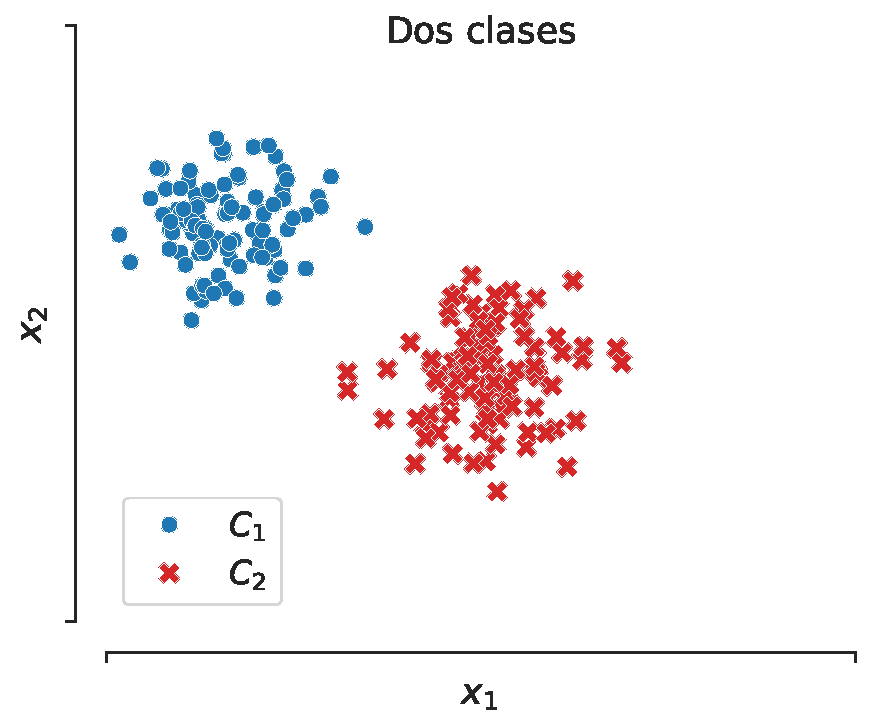
\includegraphics[width=\textwidth]{img/cap3_dosclases}\\
	\captionof{figure}{Ejemplo del problema  de clasificación binaria, donde la clase $\cC_1$ está presentada en azul y la clase $\cC_2$ en rojo.}
	\label{fig:puntos_2d}
\end{minipage}

\vspace{1cm}


Para resolver el problema de clasificación, debemos encontrar los parámetros $a$ y $b$ en la ec.~\eqref{eq:clasificacion_lineal}. Para este fin, veamos que si $x_1,x_2$ son dos puntos en la superficie de decisión, entonces tenemos la siguiente relación para el parámetro $a$:
\begin{align}
	0 &= y(x_1) - y(x_2) \nonumber\\
	  &= a^\top x_1 + b - a^\top x_2 - b \nonumber\\
	  &= a^\top (x_1-x_2).
\end{align}

Es decir, $a$ es ortogonal a cualquier vector que esté contenido dentro de la región de decisión (ya que $x_1-x_2$ corresponde a un vector director del hiperplano). Intuitivamente, podemos decir que el vector $a\in\R^M$ controla la pendiente (o inclinación) del hiperplano de decisión. Además, observemos que para cualquier $x$ en la región de decisión, i.e., $y(x)=0$,  su proyección en el vector $a$ está dada por 
	
	\begin{equation}
	\norm{\text{proy}_a(x)} = \norm{x}cos(\theta) = \norm{x} \frac{a^\top x}{\norm{a}\cdot\norm{x}} = -\frac{b}{\norm{a}}
\end{equation}


\begin{figure}[h]
    \centering
    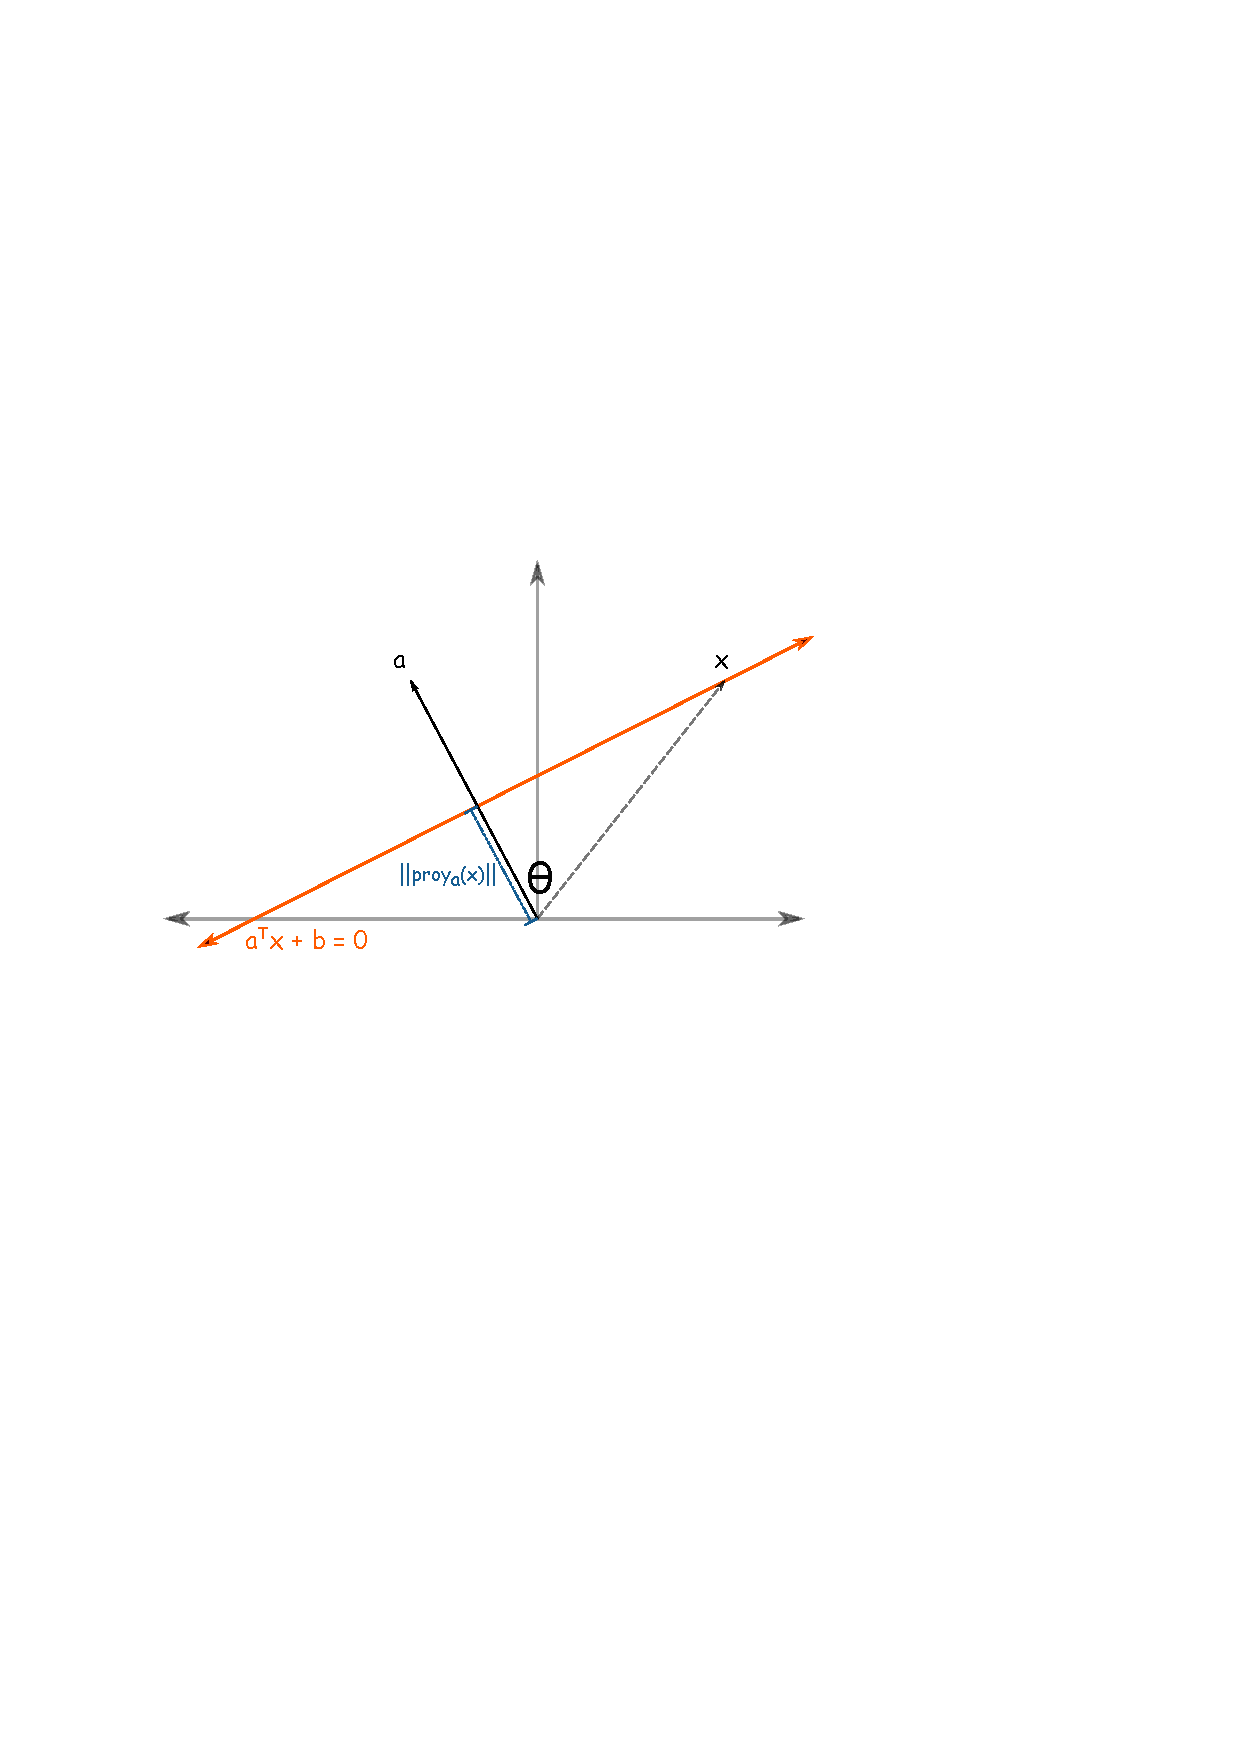
\includegraphics[width=0.5\textwidth]{img/cap3_proy.pdf}
    \caption{Proyección de un punto sobre la región de decisión. }
\end{figure}

Donde se usó el hecho de que $\cos\left(\measuredangle(x,y)\right) = \frac{\langle x,y\rangle}{\norm{x}\norm{y}}$.


Por lo tanto, se concluye que el parámetro $b$ controla el desplazamiento (o ubicación) de la región de decisión,  pues el lado izquierdo de la ecuación representa la distancia entre la región de decisión y el origen: $\norm{\text{proy}_a(x)} = d(\{x:a^\top x+b = 0\},0)$.\\

Es posible  también interpretar $y(x)$ como una distancia con signo entre un $x\in\R^M$ cualquiera  y la superficie de decisión. Para ver esto, consideremos $x\in\R^M$ y descompongámoslo dos componentes: la primera denotada por $x_{\bot}$, la cual es la proyección ortogonal de $x$ en el hiperplano de  decisión, y la segunda que es perpendicular al hiperplano (y consecuentemente paralela al vector $a$) denotada por $r\frac{a}{\left \| a \right \|}$, donde $r$ denota la distancia entre $x$ y el  hiperplano de  decisión. Expresamos entonces  
\begin{equation}
	x = x_{\bot}+r\frac{a}{\left \| a \right \|},
\end{equation}
y observamos que
\begin{equation}
	y(x) 
	= a^\top x+b 
	=a^\top  \left( x_{\bot} + r\frac{a}{\left \| a \right \|} \right) +b 
	= \underbrace{a^\top x_{\bot} +b }_{=0} +   r\frac{a^\top  a}{\left \| a \right \|}
	= r||a||.
\end{equation}
Consecuentemente, vemos que $\forall x\in\R^M$, $r = \frac{y(x)}{||a||}$,  es decir, $y(x)$ representa una medida con signo de la  distancia entre el punto $x$ y la  región de decisión (ya que $r$ lo es).\\

El caso de múltiples clases ($K>2$) puede ser enfrentado mediante una extensión del caso binario. Una forma puede ser construir $K-1$ clasificadores binarios, en donde cada uno  resuelve el problema de discriminar los elementos de la  clase $\cC_k$ del resto; esta técnica se llama \emph{one-versus-rest} (OvR). Otra forma es construir $K(K-1)/2$ clasificadores binarios, donde cada uno discrimina entre cada posible par de clases; esta técnica se llama \emph{one-versus-one} (OvO). El problema con estas dos alternativas es que dejan  regiones indefinidas en el espacio, pues solo consideran pares de clases que  al ser agregados pueden ser incoherentes. \\

Una alternativa más robusta para resolver el problema de clasificación multiclase es construir un clasificador para $K$ clases que contiene $K$ funciones lineales de la forma
\begin{equation}
	y_k(x) = a_k^\top x + b_k, \quad k=1,\ldots,K.
\end{equation}
Donde $x$ es asignado a la clase $\mathcal{C}_k$ si y solo si $y_k(x) > y_j(x), \forall j\neq k$, es decir:

\begin{equation}
	\mathcal{C}(x) = \underset{k}{\argmax}\hspace{1mm} y_j(x).
\end{equation}

Además, las $K$ componentes de la partición del espacio generada por este clasificador son convexas ya que es intersección finita de semiespacios (poliedro). Además, ningún punto del espacio queda sin clasificar ya que la clase queda determinada por el máximo de un conjunto finito. Por otra parte, el conjunto de puntos con más de una clase asignada tiene medida cero ya que las fronteras de decisión son subconjuntos de codimensión 1 (hiperplanos).\\

Por último, tomando $K=2$, se obtiene el clasificador  binario.

\subsubsection{Ajuste mediante mínimos cuadrados}

Ya hemos planteado el modelo y analizado el rol  y significado de cada uno de sus parámetros; ahora queda por estudiar cómo determinar dichos parámetros $a$ y $b$, dado un conjunto de datos $\datos$. Para esto consideraremos en primer lugar el enfoque de mínimos cuadrados, el cual es la medida de discrepancia  por  excelencia  y a primera vista  parece una respuesta natural a este problema. Primero  introduciremos un poco de notación para plantear el problema de forma clara.

Consideremos el  punto $x\in\R^M$ con clase $c\in\{\mathcal{C}_k\}_{k=1}^K$. Usaremos la \emph{codificación} $t \in\{0,1\}^K$ para representar la pertenencia de $x$ a su respectiva clase. Es decir, 
\begin{equation}
	c = \cC_j \Leftrightarrow [t]_j=1 \wedge [t]_i=0, \quad i\neq j.
\end{equation}
Este tipo de codificación  es conocida como \emph{one-hot  encoding.}  

\begin{remark}
Usamos esta codificación por  dos razones. Primero, para poder dar valores numéricos a la clase y que  podamos hablar de distancias entre ellos, pues si nuestras clases son ``peras y manzanas'' necesitamos poder determinar cuán cerca a cada una de ellas está nuestra estimación. En segundo  lugar, como los valores asignados al vector $t$ siempre serán puros 0's y un solo 1, entonces  todos los posibles  valores de $t$ están a la misma distancia unos de otros. De esta forma, si dos elementos tienen distintas clases, la distancia entre estas, cualquieras sean, será 0 (clases iguales), o bien $\sqrt{2}$ (clases distintas). Esto ayuda a no introducir sesgos en la representación de la clase que puedan alterar el aprendizaje del modelo.  	
\end{remark}

Asumiendo entonces un modelo lineal para cada clase $\mathcal{C}_k$, se tiene que
\begin{equation}
	y_k(x) = a_k^\top x + b_k = \tilde{\theta}_k^\top\tx, \quad \text{donde } \tx = \left( \begin{matrix} x\\ 1 \end{matrix}\right)\in\R^{M+1} ,\quad
  \tilde{\theta}_k = \left( \begin{matrix} a_k\\ b_k \end{matrix}\right)\in\R^{M+1}
\end{equation}

Lo anterior se puede unir en un único sistema matricial:

\begin{equation}
\tilde{\Theta} = \left(\theta_1,\cdots,\theta_K\right)\in\R^{(M+1)\times K} \implies  y(x) = \left( \begin{matrix}y_1(x) \\\vdots \\ y_K(x) \end{matrix}\right) = \tilde{\Theta}^\top \tilde{x}.
  \end{equation}
  


Donde ahora $y$ corresponde al vector de \emph{asignaciones de clases}. De esta forma, un punto $x$ será asignado a la clase que tenga mayor $y_k=\tilde{\theta}_k^\top \tilde{x}$. Es  decir, la clase de $x$ es modelada como  el  $\argmax_k y_k(x)$.\\

Con la notación establecida, ahora podemos enfocarnos en el entrenamiento del modelo.  Para esto consideremos un conjunto de entrenamiento $\{(x_n,t_n)\}_{n=1}^N$. El enfoque de entrenamiento será el correspondiente a mínimos cuadrados asociado al error de asignación:

\begin{equation}
	J = \sum_{i=1}^N \norm{t_i - \tilde{\Theta}^\top\tx_i}_2^2
\end{equation}

Por otra parte, definiendo las siguientes matrices:

\begin{equation}
	T = \left(\begin{matrix}
		t_1^\top\\
		\vdots\\
		t_N^\top
	\end{matrix}\right)\in\R^{N\times K},\qquad
	\tX = \left(\begin{matrix}
		\tx_1^\top\\
		\vdots\\
		\tx_N^\top
	\end{matrix}\right)\in\R^{N\times (M+1)}
\end{equation}

se tiene el siguiente resultado:

\begin{lemma}
	Bajo la notación anterior, $J=\operatorfont{Tr} \left((\tX\tilde{\Theta}-T)^\top (\tX\tilde{\Theta}-T)\right)$ y su mínimo es alcanzado en: 
	\begin{equation}
		\tilde{\Theta} = (\tilde{X}^\top\tilde{X})^{-1}\tilde{X}^\top T
	\end{equation}
	donde $\operatorfont{Tr}$ corresponde al operador traza: $A\in\R^{n\times n}\mapsto \operatorfont{Tr}(A):=\sum\limits_{i=1}^n a_{ii}$.
\end{lemma}

\begin{proof}
\begin{align}
	J &= \sum_{i=1}^N \norm{t_i - \tilde{\Theta}^\top\tx_i}_2^2 = \sum_{i=1}^N \norm{\left(T - \tX\tilde{\Theta}\right)_{i\cdot}}_2^2 = \sum_{i=1}^N \sum_{j=1}^K \left(T - \tX\tilde{\Theta}\right)_{ij} \left(T - \tX\tilde{\Theta}\right)_{ij}\\
	&= \sum_{i=1}^N \sum_{j=1}^K \left(T - \tX\tilde{\Theta}\right)^\top_{ji} \left(T - \tX\tilde{\Theta}\right)_{ij} =  \sum_{j=1}^K \left[\left(T - \tX\tilde{\Theta}\right)^\top \left(T - \tX\tilde{\Theta}\right)\right]_{jj}\\
	&=\operatorfont{Tr} \left((\tX\tilde{\Theta}-T)^\top (\tX\tilde{\Theta}-T)\right).
\end{align}
	
Por otra parte:
\begin{equation}
	\frac{\partial J}{\partial\tilde{\Theta}} = 2(\tX\tilde{\Theta}-T)^\top\tX=0 \iff \tilde{\Theta}^\top\tX^\top\tX - T^\top\tX = 0 \iff \tilde{\Theta}^\top = T^\top\tX(\tX^\top\tX)^{-1}\iff \tilde{\Theta} = (\tX^\top\tX)^{-1}\tX^\top T
	\end{equation}
	
Y dado que $J$ es estrictamente convexo, su mínimo se alcanza en su único punto crítico.	

\end{proof}

De acuerdo al lema anterior, la predicción de la clase para un nuevo input $x$ está dada por $ y(x) = T^\top\tilde{X}(\tilde{X}^\top\tilde{X})^{-1}\tilde{x}$.

\begin{remark}
	Para una matriz no necesariamente cuadrada $A$ se define la norma Frobenius de $A$ como $\norm{A}_F := \sqrt{\operatorfont{Tr}(A^\top A)}$. De este modo, el funcional $J$ puede ser escrito como $J = \norm{\tX\tilde{\Theta}-T}_F^2$, recuperándose la estructura de los funcionales utilizados hasta el momento: norma $l_2$ del error entre el regresor y la salida real.
	\end{remark}

\begin{remark} Hay dos problemáticas conceptuales con este enfoque. En primer lugar, el uso de mínimos cuadrados es muy sensible a la presencia de puntos aislados (\emph{outliers}). Dado el crecimiento cuadrático de la penalización, los puntos lejanos al promedio de los datos tienen una influencia mucho mayor. Esto ciertamente afecta considerablemente los resultados y no es coherente con el problema de clasificación, donde la estimación es correcta o incorrecta, pero no ``más'' o ``menos'' correcta. Este efecto sobre la solución es ilustrado en la Figura \ref{fig:clasif_mse}, en donde la presencia de puntos alejados de clase $\cC_2$ afecta el resultado (derecha), incluso donde el resultado original (izquierda) estaba correcto. En segundo lugar, las predicciones de  clase  $y(x)$ no tienen la forma de las etiquetas originales $t$, con lo cual es necesario una intervención ``manual'' en donde, dado un $y(x)$ debemos definir el $t(x)$ apropiado. 
\end{remark}


\begin{figure}[H]
	\centering
	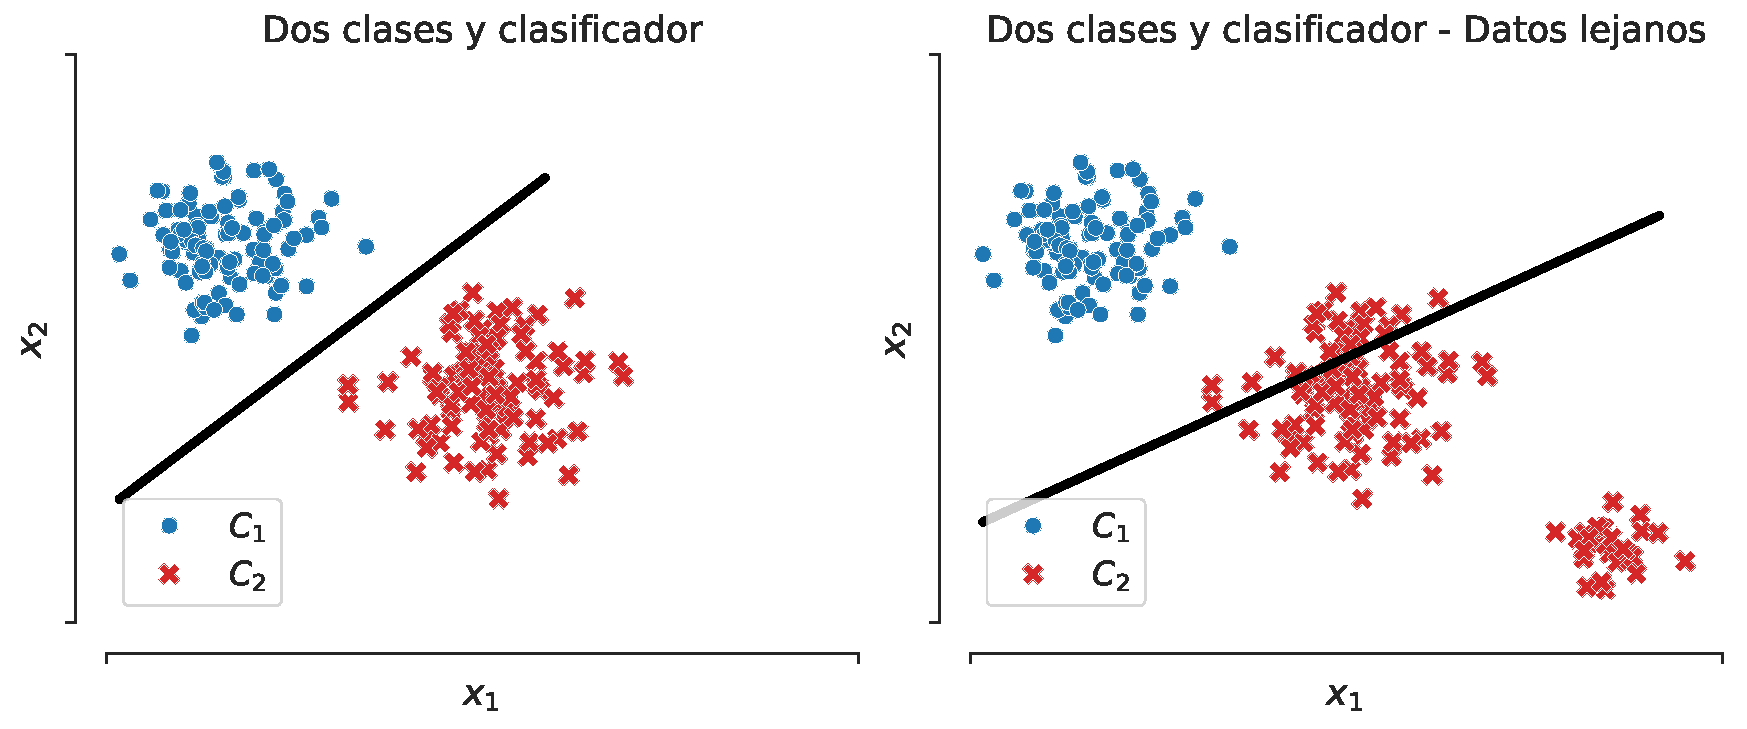
\includegraphics[width=0.8\textwidth]{img/cap3_dosclases_clasificador.pdf}\\
	\caption{Ejemplo ilustrativo sobre cómo los puntos lejanos de una clase pueden afectar incorrectamente los resultados.}
	\label{fig:clasif_mse}
\end{figure}

\subsubsection{El perceptrón}

Las nociones básicas que hemos visto hasta ahora para lidiar con el problema de clasificación tienen dos problemas conceptuales. El primero es la falta de una métrica correcta para evaluar la bondad de nuestro modelo,  esto es porque el criterios de mínimos cuadrados no es apropiado en la evaluación de una asignación de clases, donde no hay concepto de ``más cerca'', sino que solo correcto/incorrecto. Además, todos los enfoques considerados en esta sección hasta este punto no tienen una \emph{función de verosimilitud} apropiada que conecte el modelo (variables latentes) con la clase (observación) de forma coherente. Por el contrario, hasta ahora hemos considerado que por un lado tenemos el modelo lineal para clasificación y por otro lado está \emph{nuestra decisión} de la clase en base a la salida del modelo linear, por  ejemplo si $y(x)>b$ decimos que $x$ pertenece a la clase $\cC_1$.\\

La incorporación de esta función que conecta el modelo lineal con la clase, resulta en un \emph{modelo lineal generalizado}, es decir, una modelo lineal conectado a una  función no-lineal que llamaremos \emph{función de enlace}. Sin embargo, el desafío más importante en esta construcción es que el modelo resultante ya no es lineal, ni en la entrada ni en los parámetros, pues una verosimilitud (función de enlace) lineal nunca nos llevará de un espacio de inputs (hemos asumido $\R^M$) al espacio de categorías $\{\cC_1,\cC_2,\ldots,\cC_k\}$, es decir, necesitamos una no-linealidad ``después'' de la parte lineal, no antes como en el caso de los modelos lineales en lo parámetros vistos en la sección de regresión no lineal.\\

Una forma de resolver estas problemáticas es mediante el uso del \emph{Perceptrón} \cite{rosenblatt_1958}, un modelo de clasificación binario que tuvo mucha importancia en el área de reconocimiento de patrones. El Perceptrón consiste en una función no lineal fija usada para transformar $x$ en un vector de características\footnote{En este caso consideramos no linealidad antes y después de la parte lineal, sin embargo, considerar la entrada como $x$ o  como $\phi(x)$ es  equivalente en base a lo  visto en los modelos lineales en los parámetros. } $\phi(x)\in\R^D$, que luego es usado para generar un modelo lineal \emph{generalizado} con función de enlace no lineal $f(\cdot)$ de la siguiente forma:
\begin{align}
	y(x) &= f(\theta^\top\phi(x))\\
	f(u) &= \left\{\begin{matrix}
	+1,\quad u\geq 0\\
	-1,\quad u<0
	\end{matrix}\right.
\end{align}
Opciones típicas para el vector $\phi(x)$ es concatenar la entrada con un intercepto para la recta, es decir $\phi(x) = [x^\top, 1]$ y $\theta \mapsto [\theta,b]^\top$ como vimos al comienzo del curso, o bien características no lineales como las vistas en la sección de regresión no lineal. El Perceptrón entonces asigna $x$ a la clase $\mathcal{C}_1$ si $y(x)=+1$ y asignará $x$ a la clase $\mathcal{C}_2$ cuando $y(x)=-1$. Notemos que  para  el caso que $\phi$ es lineal, este es el mismo clasificador presentado en la Sección \ref{sec:clasif_lineal}, pero en este caso el criterio para asignar la clase es \textbf{parte del modelo}.\\

Una condición para determinar el parámetro $\theta\in\R^D$ en base a un conjunto de datos  $\datos = \{(x_i,t_i)\}_{i=1}^N$, es que para $x\in\mathcal{C}_1$ ($t=1$), se cumpla que $\theta^\top\phi(x) > 0$, y para $x\in\mathcal{C}_2$ ($t=-1$) se cumpla $\theta^\top \phi(x) < 0$. Usando el hecho que las etiquetas están representadas por la  codificación $t\in\{1,-1\}$, ambas condiciones pueden ser cubiertas por la expresión:
\begin{equation}
	\theta^\top\phi(x_n)t_n > 0,\quad \forall (x_n,t_n) \in \datos.
\end{equation}

Podemos entonces satisfacer esta restricción mediante el ``criterio del perceptrón'', el cual se basa en examinar  los elementos de $\datos$ que fueron clasificados incorrectamente. Este criterio asocia a los puntos clasificados correctamente error 0 y a los puntos mal clasificados error $-\theta^\top\phi(x)t>0$. De esta forma, si denotamos $\mathcal{M}$ el conjunto de puntos mal clasificados, se debe minimizar la siguiente función objetivo:


\begin{equation}
	J_\text{P}(\theta,x) = \E\left(-\theta^\top\phi(x)t(x)\mathds{1}_{\theta^\top\phi(x)t(x)\leq 0} \right) \approx -\sum_{(x_i,t_i)\in \mathcal{D}}\theta^\top\phi(x_i)t_i \mathds{1}_{\theta^\top\phi(x_i)t_i\leq 0} = -\sum_{(x_i,t_i)\in \mathcal{M}}\theta^\top\phi(x_i)t_i
\end{equation}

Para la minimización de dicho funcional, se utilizará un método no determinístico que funciona mejor que el método del gradiente clásico (ver anexos) para este tipo de funciones.


\begin{mdframed}[style=pendiente, frametitle={\center Método del gradiente estocástico}]

	En aprendizaje de máquinas por lo general se busca un parámetro óptimo que minimice el error de ajuste de acuerdo a una función de pérdida $J$. Dicho problema puede ser escrito de la forma:
	
	\begin{equation}
		\hat{\theta} = \argmin_\theta \sum_{i=1}^n J(y_i,\hat{y}_\theta(x_i) = \argmin_\theta \frac{1}{n} \sum_{i=1}^n J(y_i,\hat{y}_\theta(x_i))
	\end{equation}
	
	Donde $y_i$ corresponde a la salida de $x_i$ mientras que $\hat{y}_\theta(x_i))$ representa la predicción de la salida de $x_i$ mediante un modelo de parámetro(s) $\theta$.\\
	
	Muchas veces es infactible encontrar el óptimo de forma analítica o bien, el algoritmo del gradiente clásico se queda atrapado en mínimos locales. Una forma distinta de ver el problema es considerar que $(x_i,y_i)\sim\mu$ iid para una distribución $\mu$ desconocida. Desde ese punto de vista, el problema se reduce a minimizar $\E\left(J(y,\hat{y}_\theta(x))\right)$. Este tipo de problemas puede ser escrito en general como
	
	\begin{equation}
		\min_\theta \E(f(\theta,X)),\quad X\sim \mu\text{ desconocida}
	\end{equation}

Una alternativa al método del gradiente clásico $\theta^{\tau+1} = \theta^\tau - \beta_{\tau+1}\nabla_\theta \E(f(\theta^\tau,X))$ consiste en utilizar las observaciones iid $(x_i)_{i\geq 1}\sim\mu$ al momento de iterar, considerando una observación por iteración en vez del funcional $\E(f(\theta^\tau,X))$ completo, es decir:

\begin{equation}
	\theta^{\tau+1} = \theta^\tau - \eta_{\tau+1}\nabla_\theta f(\theta^\tau,x_{\tau+1})
\end{equation}

Donde ahora $\eta_\tau$ no necesariamente se debe calcular mediante otro problema de minimización, sino que pueden usarse secuencias heurísticas que en la práctica funcionan bien. Además, en cada iteración se necesita evaluar una sola vez $\nabla_\theta f$ y no hace falta calcular su esperanza.\\

Este método es conocido como método del gradiente estocástico (SGD), donde el término $\nabla_\theta f(\theta^\tau,x_{\tau+1})$ puede ser visto como un gradiente exacto perturbado:

\begin{equation}
	\nabla_\theta f(\theta^\tau,x_{\tau+1}) = \nabla_\theta\E(f(\theta^\tau,X)) + \Delta_t
\end{equation}

Donde $\Delta_t = \nabla_\theta f(\theta^\tau,x_{\tau+1}) - \nabla_\theta \E( f(\theta^\tau,X))$ cumple que $\E(\Delta_t)=0$ ya que de acuerdo a la regla integral de Leibniz, $\nabla_\theta \E( f(\theta^\tau,X)) =  \E(\nabla_\theta f(\theta^\tau,X))$.\\


Esta propiedad del gradiente con ruido es la que le permite al algoritmo del gradiente estocástico poder saltarse con mayor facilidad los mínimos locales ya que la evolución de $\theta_\tau$ contiene una parte aleatoria que no depende del valor del gradiente en el punto.


\begin{figure}[H]
	\centering
	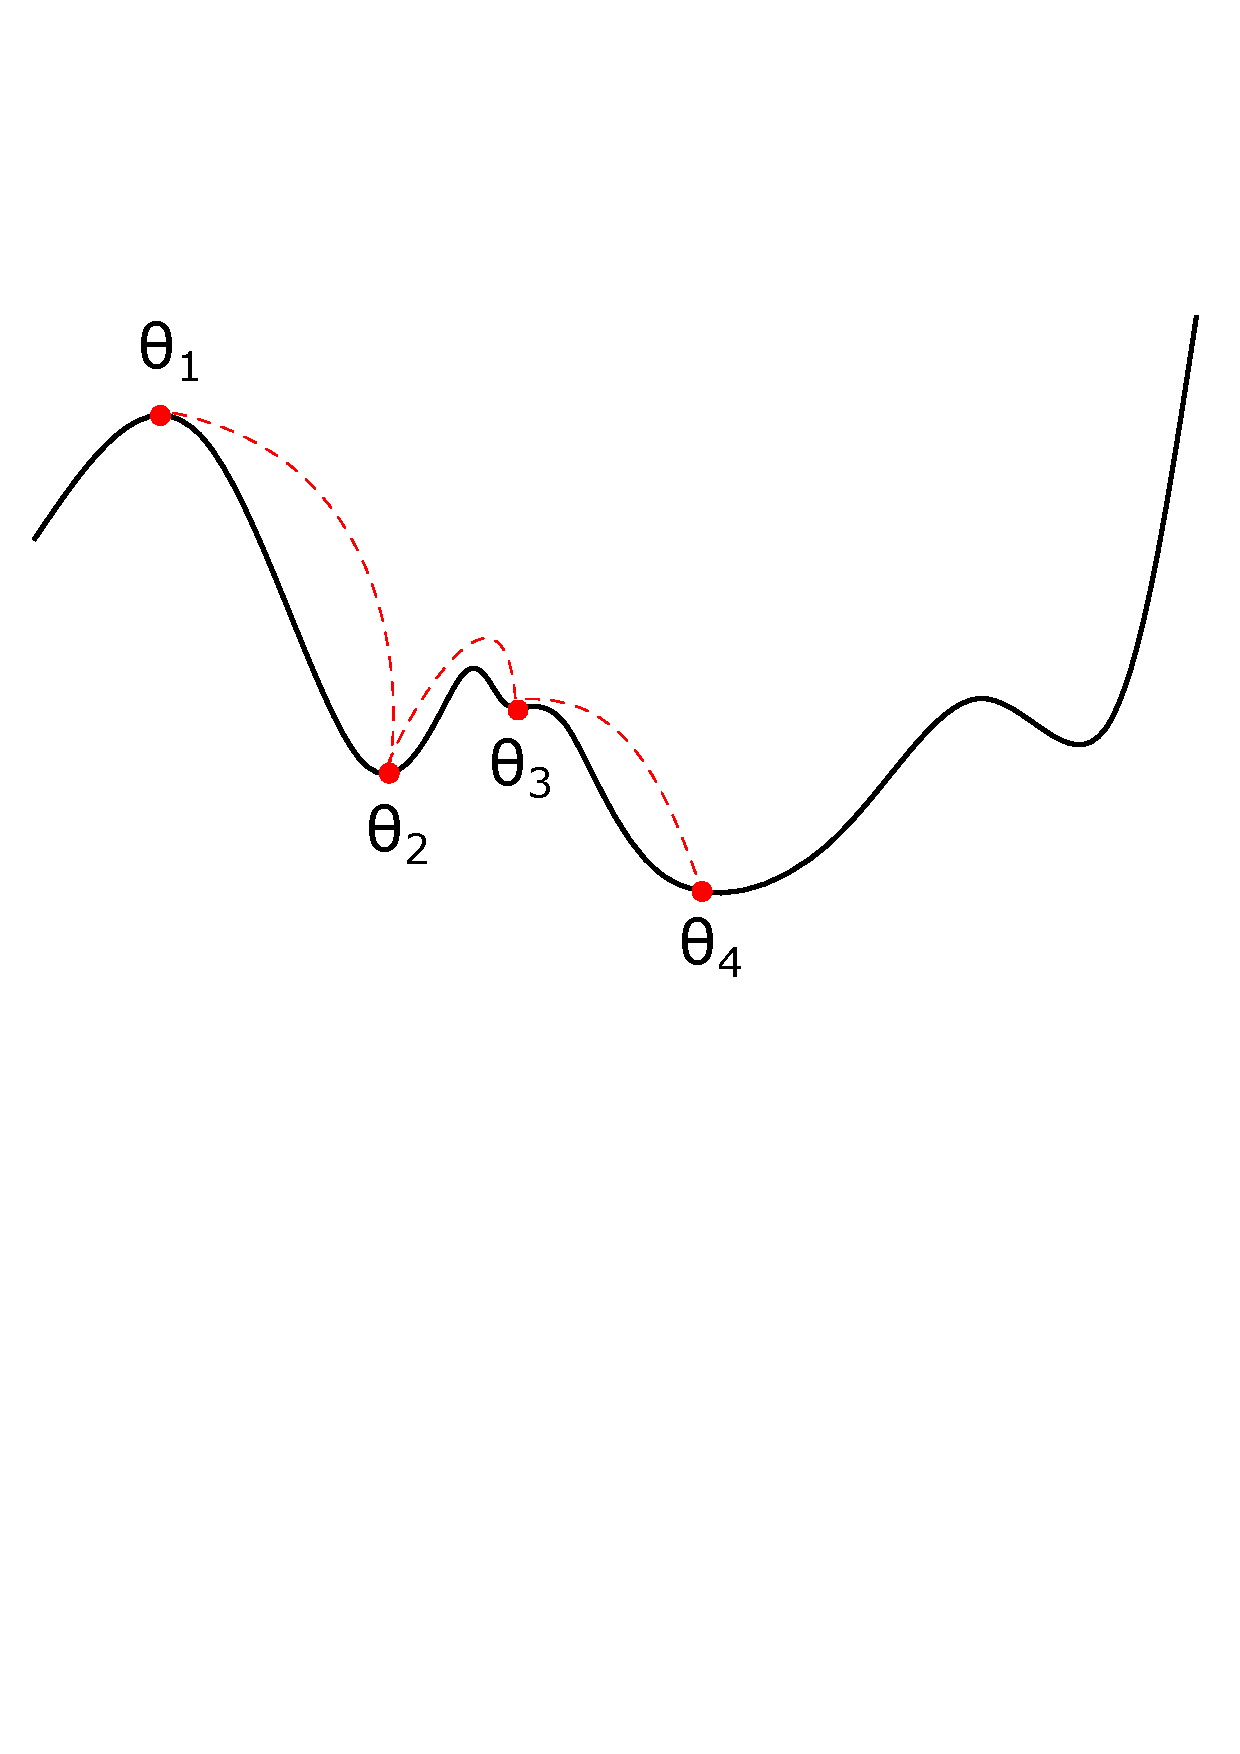
\includegraphics[width=0.6\textwidth]{img/cap3_sgd.pdf}\\
	\caption{Posibles iteraciones del algoritmo SGD. El algoritmo del gradiente clásico hubiese quedado atrapado en $\theta_2$ ya que en dicho punto el gradiente es nulo por lo que no hay desplazamiento.}
\end{figure}

Otra de las ventajas que tiene este algoritmo es que permite entrenar modelos con datos a medida que van llegando (actualización en tiempo real) y no hace falta calcular el funcional de optimización utilizando todos los datos anteriores.\\

Si bien no está garantizada la convergencia a un óptimo global, este método funciona bien en la práctica mediante secuencias probadas de $(\eta_\tau)$ (learning rate). Una selección usual es usar $\eta_\tau$ constante o constante por tramos.\\

Un resultado teórico simple acerca del SGD es el siguiente:


	\begin{theorem}[Sigmund-Robins] Bajo hipótesis razonables sobre $f$ (regularidad en $\theta$, integrabilidad de $\nabla_\theta f$ y cotas) y tasas de aprendizaje suficientemente pequeñas (por ejemplo, $\eta_\tau = 1/\tau$), la sucesión $(\theta^\tau)_{\tau\geq 1}$ converge c.s. al conjunto de puntos críticos de $\E(f(\theta,X))$.\\		
	\end{theorem}
	
En particular, para $f$ convexa, la sucesión converge al conjunto de argumentos minimizantes de $\E(f(\theta,X))$.
	
\end{mdframed}

Para el problema de minimización del funcional del perceptrón, se puede utilizar el método del gradiente estocástico. En este caso, el algoritmo iterativo tiene la siguiente estructura:


\begin{align}
	\theta^{\tau+1} &= \theta^\tau - \eta_\tau \nabla_\theta J_\text{P}(\theta^\tau,x_i)\nonumber\\
	&= \theta^\tau + \eta_\tau \phi(x_i)t_i.\label{eq:percetron_rule}
\end{align}

Es importante notar que al actualizar el vector $\theta$, el conjunto de puntos mal clasificados $\mathcal{M}$ va a cambiar, pues (esperamos que) en cada iteración los elementos del conjunto de puntos mal clasificados vaya disminuyendo.\\

Por lo tanto, el algoritmo de entrenamiento para el perceptrón es el siguiente:

\begin{itemize}
	\item[i)] se recorre el conjunto de puntos de entrenamiento $\{x_i\}_{i=1}^N$,
	\item[ii)] si el punto $x_i$ fue clasificado correctamente el vector de pesos de mantiene igual
	\item[iii)] si $x_i$ fue clasificado incorrectamente, el vector $\theta^\tau$ es actualizado según la ec.~\eqref{eq:percetron_rule} con $\eta=1$ mediante
	\begin{equation}
	 \theta^{\tau+1} = \theta^\tau + \phi(x_i)t_i.
\end{equation}
\end{itemize}
Es decir, el parámetro $\theta$ está paso a paso modificado en la dirección de las características $\phi(x_i)$ con multiplicador $\pm1$ en base a la clase verdadera de $x_i$ hasta  que todos los puntos de $\datos$ están bien clasificados. 




\subsection{Clasificación probabilística: modelo generativo}

Los modelos que hemos revisado hasta este punto son del tipo \emph{discriminativo}, es decir, modelan directamente la función $f:x\mapsto c$. Con una interpretación probabilística, esto es equivalente a modelar la probabilidad condicional $\mathbb{P}(\mathcal{C}_k|x)$, es decir, dado que conozco el input (o características de) $x$, cuál es la distribución de probabilidad sobre las clases. Sin embargo, hemos considerado métodos determinísticos, que solo asignan probabilidad 1 a una sola clase. 


Un paradigma alternativo es considerar es un enfoque \emph{generativo}, en el cual modelamos dos  objetos: en primer lugar la ``probabilidad condicional de clase'' la cual representa cómo distribuyen los valores de los inputs $x$ cuando la  clase es, por  ejemplo, $\cC_k$, denotada por $\mathbb{P}(x|\mathcal{C}_k)$. En segundo lugar las ``probabilidades de clase'', o el prior sobre clases, denotada $\mathbb{P}(\mathcal{C}_k)$. Luego, podemos calcular la densidad posterior sobre las clases dado un input $x$ usando el Teorema de Bayes de acuerdo a 
\begin{equation}
	\mathbb{P}(\mathcal{C}_k|x) = \frac{\mathbb{P}(x|\mathcal{C}_k)\mathbb{P}(\mathcal{C}_k)}{\mathbb{P}(x)}.
\end{equation}

Para el caso de 2 clases, es posible calcular la probabilidad de la clase $\cC_1$ dado $x$ de la forma:
\begin{align}
	\mathbb{P}(\mathcal{C}_1|x) 
	&= \frac{\mathbb{P}(x|\mathcal{C}_1)\mathbb{P}(\mathcal{C}_1)}{\mathbb{P}(x)}\nonumber\\
	&= \frac{\mathbb{P}(x|\mathcal{C}_1)\mathbb{P}(\mathcal{C}_1)}{\mathbb{P}(x|\mathcal{C}_1)\mathbb{P}(\mathcal{C}_1)+\mathbb{P}(x|\mathcal{C}_2)\mathbb{P}(\mathcal{C}_2)}\nonumber\\
	&=\frac{1}{1+\frac{\mathbb{P}(x|\mathcal{C}_2)\mathbb{P}(\mathcal{C}_2)}{\mathbb{P}(x|\mathcal{C}_1)\mathbb{P}(\mathcal{C}_1)}}\nonumber\\
	&=\frac{1}{1+\exp(-r)} = \sigma(r).\label{eq:logistic1}
\end{align}
Donde hemos introducido la notación $r = r(x) =\ln\left(\frac{\mathbb{P}(x|\mathcal{C}_1)\mathbb{P}(\mathcal{C}_1)}{\mathbb{P}(x|\mathcal{C}_2)\mathbb{P}(\mathcal{C}_2)}\right)$  y la  función logística definida mediante $\sigma(r) = \frac{1}{1+e^{-r}}$, la cual  tiene propiedades que serán útiles en el entrenamiento, en particular:
\begin{align}
	\text{reflejo: }\sigma(-r)&=1-\sigma(r)\\
	\text{derivada: }\frac{d}{dr}\sigma(r)&=\sigma(r)(1-\sigma(r))\\
	\text{inversa: }r(\sigma)&=\ln\left(\frac{\sigma}{1-\sigma}\right).
\end{align}


\begin{remark} Si bien la expresión de la distribución condicional en la ec.~\eqref{eq:logistic1} parece una presentación antojadiza para hacer aparecer la  función logística (sigmoide), pues $r=r(x)$ puede ser cualquier cosa. Sin embargo, veremos que existe una elección particular de las distribuciones condicionales de clase que lleva a un $r$ que es efectivamente lineal en $x$. En general, nos  referiremos a este clasificador como \textbf{regresión logística} en dicho caso, es decir, cuando $r(x) = a^\top x  + b$.
\end{remark} 

Podemos ahora considerar el caso de múltiples clases $\{\cC_1,\ldots,\cC_K\}$, donde un desarrollo similar al anterior resulta en:  
\begin{equation}
	\mathbb{P}(\mathcal{C}_i | x) = \frac{\mathbb{P}(x | \mathcal{C}_i)\mathbb{P}(\mathcal{C}_i)}{\sum_{j}\mathbb{P}(x | \mathcal{C}_j)\mathbb{P}(\mathcal{C}_j)} = \frac{\exp(s_i)}{\sum_{j}\exp(s_j)},\label{eq:softmax1}  
\end{equation}
donde hemos denotado $s_i = \log\left(\mathbb{P}(x | \mathcal{C}_i)\mathbb{P}(\mathcal{C}_i)\right)$. La función que aparece al lado derecho de la  ec.~\eqref{eq:softmax1} se conoce como \emph{exponencial normalizada} o \emph{softmax}, y corresponde a una generalización de la función logística a múltiples clases. Además, esta función tiene la propiedad de ser una aproximación suave de la función máximo y convertir cualquier vector $s=[s_1,\ldots,s_k]$ en una distribución de probabilidad, donde podemos hablar de ``la probabilidad de ser clase $\cC_k$''.

\subsubsection{Regresión logística} 
\label{sub:reg_log}

Analizaremos ahora  los supuestos sobre el modelo generativo (i.e., las  probabilidades de clase y condicionales) para encontrar un $r$ --en la ec.~\eqref{eq:logistic1}-- que resulta en la bien conocida regresión logística. Consideraremos el caso binario donde las densidades condicionales de clase son Gaussianas multivariadas, dadas por
\begin{equation}
	p(x|\mathcal{C}_k) \sim \mathcal{N} (\mu_k,\Sigma) = \frac{1}{(2\pi)^\frac{D}{2}|\Sigma|^\frac{1}{2}}\exp(-\frac{1}{2}(x-\mu_k)^\top \Sigma^{-1}(x-\mu_k))\quad k\in\{1,2\}.
\end{equation}

Donde $u_k\in\R^M$ corresponde al centroide de la clase $\mathcal{C}_k$ y $\Sigma\in\R^{M\times M}$ simétrica y definida positiva, corresponde a la matriz de covarianza de las clases (misma matriz para todas las clases). Para este caso, se tiene que para la ecuación \eqref{eq:logistic1}:

\begin{align}
r &= \ln\left(\frac{\mathbb{P}(x|\mathcal{C}_1)\mathbb{P}(\mathcal{C}_1)}{\mathbb{P}(x|\mathcal{C}_2)\mathbb{P}(\mathcal{C}_2)}\right) = \ln\left(\frac{\exp(-\frac{1}{2}(x-\mu_1)^\top \Sigma^{-1}(x-\mu_1))\mathbb{P}(\mathcal{C}_1)}{\exp(-\frac{1}{2}(x-\mu_2)^\top \Sigma^{-1}(x-\mu_2))\mathbb{P}(\mathcal{C}_2)}\right)\\
&= -\frac{1}{2}(x-\mu_1)^\top \Sigma^{-1}(x-\mu_1) +\frac{1}{2}(x-\mu_2)^\top \Sigma^{-1}(x-\mu_2) + \ln\left(\frac{p(\mathcal{C}_1)}{p(\mathcal{C}_2)}\right)\\
&= \frac{1}{2}\left(x^\top\Sigma^{-1}(\mu_1-\mu_2) + (\mu_1-\mu_2)^\top\Sigma^{-1}x - \mu_1\Sigma^{-1}\mu_1 + \mu_2\Sigma^{-1}\mu_2 \right) + \ln\left(\frac{p(\mathcal{C}_1)}{p(\mathcal{C}_2)}\right)\\
&= (\mu_1-\mu_2)^\top\Sigma^{-1}x + \frac{1}{2}\left(\mu_2\Sigma^{-1}\mu_2 - \mu_1\Sigma^{-1}\mu_1 \right)+ \ln\left(\frac{p(\mathcal{C}_1)}{p(\mathcal{C}_2)}\right)\\
&= a^\top x+b
\end{align}

donde hemos usado la notación
\begin{align}
a &= \Sigma^{-1}(\mu_1-\mu_2)\\
b &= \frac{1}{2}(\mu_2^\top \Sigma^{-1}\mu_2-\mu_1^\top \Sigma^{-1}\mu_1)
+\ln\left(\frac{p(\mathcal{C}_1)}{p(\mathcal{C}_2)}\right). 
\end{align}

y el hecho de que $\Sigma^{-1}$ es simétrica.\\

Lo anterior nos entrega la regresión logística (lineal) para el  caso binario, donde al incorporar la expresión anterior en la ec.~\eqref{eq:logistic1} obtenemos
\begin{equation}
	p(\mathcal{C}_k|x) = \sigma(a^\top x+b) = \frac{1}{1 + \exp{\left(-a^\top x-b\right)}}. \label{eq:logistica2}
\end{equation}

\begin{remark}
	La reducción de $r$ a una forma lineal prueba que es necesario considerar matrices de covarianza $\Sigma$ iguales para todas las clases, ya que de lo contrario no se podrían simplificar los términos cuadráticos $x^\top\Sigma^{-1}x$.
\end{remark}

\begin{remark}\label{rem:reg_log} 
El modelo de clasificación binaria en la  ec.~\ref{eq:logistica2} es conocido como \emph{regresión logística} y es la consecuencia de asumir un modelo generativo Gaussiano con distintas medias pero la misma varianza para una de las clases. Como consecuencia, la región de decisión se encuentra imponiendo que la probabilidad de ser clase $\cC_1$ sea 1/2 (y por ende, ser $\cC_2$ también tiene probabilidad 1/2), lo cual se tiene para 
\begin{equation}
	a^\top x+b = 0.
\end{equation}
\end{remark}

Ahora que hemos definido el modelo para nuestro problema de clasificación, aflora naturalmente la siguiente pregunta: ¿Cómo ajustar los parámetros de las condicionales a la clase y priors respectivamente? Para esto, reiteremos que los parámetros del modelos serán los de la probabilidad de clase $p(\cC_k)$ y de la probabilidades condicionales de clase $p(x|\cC_k)$. Respectivamente: 

\begin{itemize}
	\item Probabilidad de clase:
	\begin{equation}
	 	p(\mathcal{C}_1)=\pi,\quad  p(\mathcal{C}_2)=1-\pi,\label{eq:prob_clase}
	 \end{equation}  es decir,  un parámetro $\pi$ (por determinar).
	\item Probabilidad condicional de clase:
	\begin{equation}
		p(x|\mathcal{C}_k) = \mathcal{N}(\mu_k,  \Sigma); k=1,2,\label{eq:prob_clase_cond}
	\end{equation} 
	es decir, parámetros $ \mu_1\in\R^M,\mu_2\in\R^M,\Sigma\in\R^M\times\R^M$ (por determinar) o, equivalentemente, $M + M + M(M+1)/2=M(M+5)/2$ parámetros escalares (considerando que $\Sigma$ es simétrica). 
\end{itemize}
Denotaremos todos los parámetros mediante el parámetro agregado $\theta =\{\pi,\mu_1,\mu_2,\Sigma \}$.\\

Realizaremos el entrenamiento del modelo, i.e., encontrar $\theta$ en base a un conjunto de datos $\datos$, mediante el método de máxima verosimilitud. Para esto, notemos que solo hemos definido ``la probabilidad de ser clase $\cC_1$'', noción que extendemos usando la codificación de clases $t\in\{0,1\}$.  Con esta codificación, donde la observación $(x_i,t_i)$ corresponde a clase $\cC_1$ con $t_i = 1$ y a clase $\cC_2$ con  $t=0$, podemos expresar la verosimilitud con una observación mediante:
\begin{equation}
	L_i(\theta) = p(x_i, t_i|\theta) =  p(x_i,\cC_1|\theta)^{t_i}p(x_i,\cC_0|\theta)^{1-t_i}. 
\end{equation}
Esta expresión equivale a la probabilidad de ser clase $\cC_1$ cuando $t_i=1$ y a la probabilidad de ser clase $\cC_0$ cuando $t_i=0$. Consecuentemente, para un conjunto de datos $\datos$ de la forma

\begin{equation}
X=\left(\begin{matrix}
		x_1^\top\\ \vdots\\ x_N^\top
	\end{matrix}\right)\in\R^{N\times M},\qquad
	T=\left(\begin{matrix}
		t_1\\ \vdots\\ t_N
	\end{matrix}\right)\in\{0,1\}^N \text{ es decir, codificación $0-1$.}
\end{equation}

podemos escribir la verosimilitud mediante $L(\theta) = p(X,T|\theta) $, luego:
\begin{align}
	L(\theta) &= \prod_{i=1}^{N}p(x_i,t_i|\theta)
	= \prod_{i=1}^{N}p(x_i,\mathcal{C}_1|\theta)^{t_i}p(x_i,\mathcal{C}_0|\theta)^{1-t_i}\\
	&=\prod_{i=1}^{N}\left(p(x_i|\mathcal{C}_1,\theta)p(\mathcal{C}_1|\theta)\right)^{t_i}\left(p(x_i|\mathcal{C}_0,\theta)p(\mathcal{C}_0|\theta)\right)^{1-t_i}\\
	&= \prod_{i=1}^{N}(\pi\mathcal{N}(x_i|\mu_1,\Sigma))^{t_i}
	((1-\pi)\mathcal{N}(x_i|\mu_2,\Sigma))^{1-t_i}.
	\end{align}

Al igual que en el escenario de regresión lineal, para proceder con la optimización nos enfocamos en la log-verosimilitud, dada por:	
	\begin{equation}
	l(\theta) := \log L(\theta) = \sum_{i=1}^{N}\left(t_i(\log(\pi)+\log(\mathcal{N}(x_i|\mu_1,\Sigma)))+(1-t_i)(\log(1-\pi)+\log(\mathcal{N}(x_i|\mu_2,\Sigma)))\right) 
		\end{equation}

Aplicando entonces las condiciones de primer orden, tenemos que 
\begin{itemize}
	
\item \textbf{1)} Con respecto a $\pi$:
	
	\begin{align}
	\frac{\partial\log(L)}{\partial\pi} &= \sum_{i=1}^N \frac{t_i}{\pi}-\frac{1-t_i}{1-\pi}=0\nonumber\\
	\Rightarrow \quad & (1-\pi)\sum_{i=1}^Nt_i = \pi\sum_{i=1}^N(1-t_i)\nonumber\\
	\Rightarrow \quad & \sum_{i=1}^Nt_i=\pi N \quad\Rightarrow\quad \pi = \frac{\sum_{i=1}^Nt_i}{N} = \frac{N_1}{N_1+N_2} \label{eq:log_reg_pi}
	\end{align}
	
	Donde $N_i:=\text{Card}(x:x\in\mathcal{C}_i)$. Por lo tanto, el EMV de $pi$ colapsa a la regla de Laplace.
	
\item \textbf{2)} Con respecto a $\mu_1$:
	
	\begin{align}
	\frac{\partial\log(L)}{\partial\mu_1} &= \sum_{i=1}^N t_i
	\frac{\partial}{\partial \mu_1}(-\frac{1}{2}(x_i-\mu_1)^\top \Sigma^{-1}(x_i-\mu_1))\nonumber\\
	&= \sum_{i=1}^N t_i(\Sigma^{-1}(x_i-\mu_1)) =
	\Sigma^{-1}\sum_{i=1}^N t_i(x_i-\mu_1) = 0\nonumber\\
	\Rightarrow\quad & \sum_{i=1}^Nt_ix_i= \mu_1\sum_{i=1}^N t_i
	\quad\Rightarrow\quad \mu_1  = \frac{1}{N_1}\sum_{i=1}^Nt_ix_i = \frac{1}{N_1}\sum_{x_i\in \mathcal{C}_1}x_i \label{eq:log_reg_mu1}
	\end{align}
	
	De forma análoga:
	\begin{equation}
	\mu_2 = \frac{1}{N_2}\sum_{x_i\in \mathcal{C}_2}x_i \label{eq:log_reg_mu2}
	\end{equation}
	
\end{itemize}

\begin{remark}\label{rem:log_reg_interpretacion_ML}
La ec.~\eqref{eq:log_reg_pi} revela que el parámetro  óptimo $\pi$ es precisamente la razón entre la cantidad de elementos de la clase $\cC_1$ y el total de datos, esto es porque $\pi$ es la probabilidad de ser clase $\cC_1$; lo mismo aplica para $(1-\pi)$ y clase $\cC_0$. Además, de las ecs.~\eqref{eq:log_reg_mu1}-\eqref{eq:log_reg_mu2} vemos también que el estimador de MV para la media de las clases es la media muestral de los datos disponibles por cada clase. Queda la siguiente pregunta entonces: ¿cuál es el estimador de MV de $\Sigma$?
\end{remark}

\subsubsection{Regresión logística v/s modelo generativo}

Recordemos que los supuestos tomados sobre el modelo generativo para el problema de clasificación resultaron en:
\begin{equation}
p(\mathcal{C}_1|x) = \sigma(w^\top x) = \frac{1}{1+e^{-w^\top x}} \label{eq:log_reg_discriminativo},
\end{equation}
donde por claridad de notación hemos elegido la representación lineal $(w^\top x)$ y no afín $(a^\top x + b)$. 

En el caso anterior se ha entrenado el modelo generativo completo, es decir, $\pi, \mu_1,\mu_2, \Sigma$, lo cual tiene la ventaja de tener solución en forma cerrada, sin embargo, puede ser innecesario cuando solo necesitamos conocer el peso $w$ en la ecuación anterior. Otra forma de entrenar la  regresión logística es considerar el modelo discriminativo en la  ec.~\eqref{eq:log_reg_discriminativo} y optimizar directamente la verosimilitud sobre  este modelo para encontrar $w$; en vez de todos los parámetros $\pi,\mu_1,\mu_2,\Sigma$ del modelo generativo.

Calculemos la verosimilitud de la regresión logística con datos $\datos=\{(x_i,t_i)\}_{i=1}^N$, para hacer la notación más compacta denotamos $\sigma_i = \sigma(w^\top x_i)$. Entonces:
\begin{equation}
p((t_i)_{i=1}^N|(x_i)_{i=1}^N,w) = \prod_{i=1}^{N}p(t_i|x_i,w)= \prod_{i=1}^{N} p(\mathcal{C}_1|x_i)^{t_i} p(\mathcal{C}_2|x_i)^{1-t_i} =  \prod_{i=1}^{N}\sigma_i^{t_i}(1-\sigma_i)^{1-t_i} 
\end{equation}
Con lo que la log-verosimilitud está dada por
\begin{equation}
	l(w) = \sum_{i=1}^N t_i\log(\sigma_i) + (1-t_i)\log(1-\sigma_i).
\end{equation}

Notemos que este  problema de optimización no exhibe una solución en forma cerrada, por lo que podemos resolverlo mediante gradiente, para lo cual es necesario calcular el gradiente de $l(w)$ respecto a $w$:
\begin{align}
\nabla_w l(w) = \sum_{i=1}^N (t_i-\sigma_i)x_i,
\end{align}
lo cual nos da una regla de  ajuste $\theta \mapsto \theta - \eta \sum_{i=1}^N (\sigma_i-t_i)x_i$, o bien 
\begin{equation}
	\theta \mapsto \theta + \eta(t_i-\sigma_i)x_i, \label{eq:reg_log_theta_update}
\end{equation}
si tomamos los  datos de ``a uno'' (método del gradiente estocástico).
\begin{remark}\label{rem:log_reg_shocks}
Notemos que la regla de ajuste del parámetro $\theta$ en la ec.~\eqref{eq:reg_log_theta_update} recuerda el ajuste del Perceptrón en la ec.~\eqref{eq:percetron_rule}, donde los puntos mal clasificados se agregan como características al vector $\theta$. Sin  embargo, a diferencia del  perceptrón, incluso los elementos bien clasificados ($\sigma$  cercano a  1 ó 0) tomarán parte en la actualización, forzando una fuerte componente de sobreajuste al hacer tender $\theta$ a infinito. 
\end{remark}

\begin{figure}[H]
	\centering
	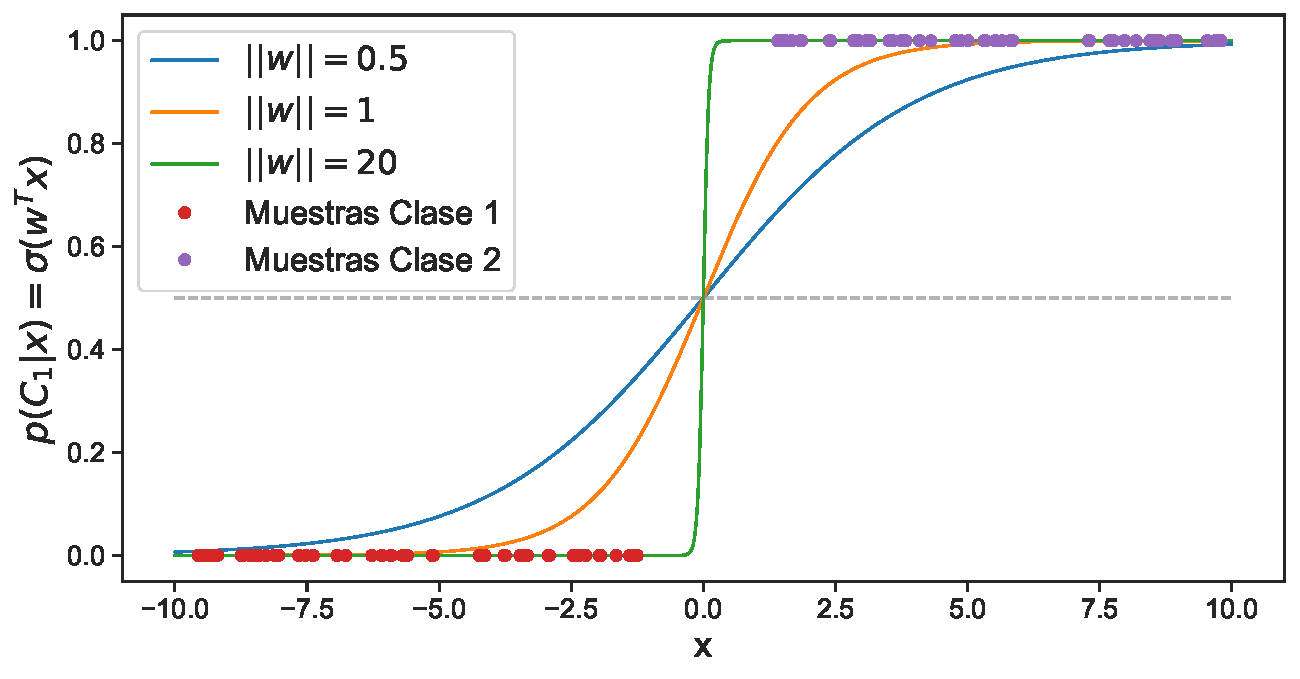
\includegraphics[width=0.9\textwidth]{img/cap3_logistica.pdf}\\
	\caption{En gris la frontera de decisión: una nueva entrada $x_\star$ será asignada a la clase $\cC_1$ si $p(\cC_1|x_\star)>\frac{1}{2}$, en caso contrario, será asignada a $\cC_2$. Se observa que al entrenar con más muestras, $\norm{w}$ crece por lo que el parámetro se sobreajusta a los datos y el clasificador converge a una función indicatriz.}
\end{figure}




%!TEX root = notas_de_clase.tex

\section{Selección y evaluación de modelos}

Dado un conjunto de datos, existen muchos posibles modelos para poder realizar el aprendizaje, por lo que surge la pregunta natural de qué modelo elegir. Una respuesta rápida a esta pregunta sería elegir el modelo que mejor se ajuste a los datos en el entrenamiento. El problema de utilizar este criterio es el sobreajuste, el cual puede ser observado en la Figura \ref{fig:overfitting} donde se observa que en la tercera imagen, el modelo aprende oscilaciones que muy probablemente son generadas por los ruidos de las observaciones. 
\begin{figure}[h!]
    \centering
    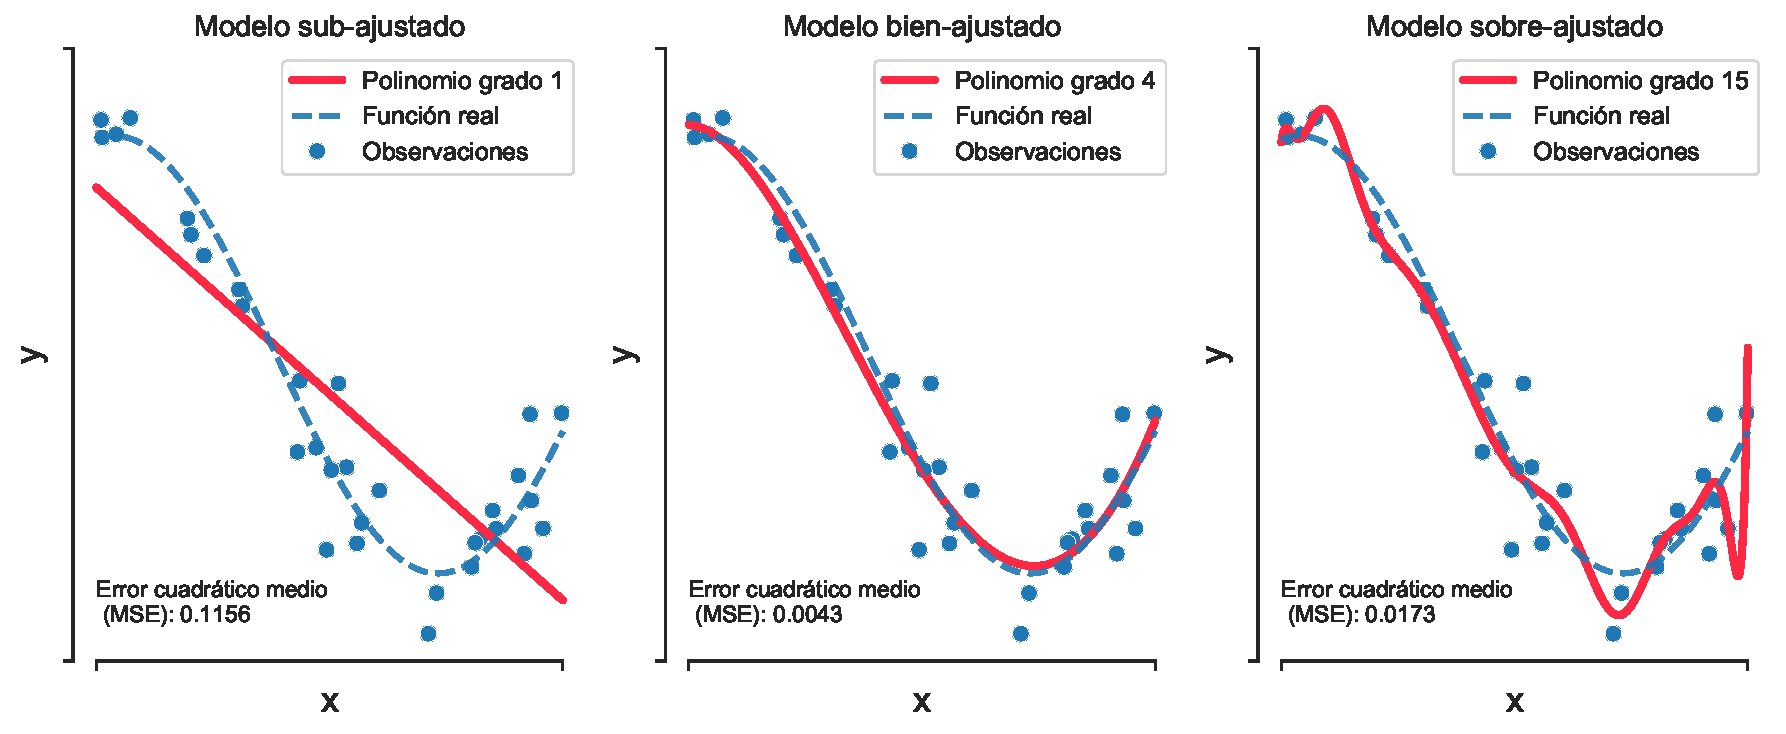
\includegraphics[width = 0.9\linewidth]{img/cap4_ajuste.pdf}
    \caption{Ejemplos de sub, sobre y correcto ajuste.}
    \label{fig:overfitting}
\end{figure}

El problema de sobreajuste ocurre, por ejemplo, en el ajuste polinomial (donde se debe elegir un cierto grado de regresión para los datos) ya que es sabido, de acuerdo al teorema de interpolación polinómica de Lagrange, que para $n$ puntos siempre existirá un polinomio de grado menor a $n$ que pase exactamente por dichos puntos, por lo que es posible tener un error de ajuste nulo en los datos de entrenamiento, pero con un alto error de predicción en datos no vistos.

\subsection{Descomposición sesgo-varianza}

En el capítulo de regresión lineal se estudió el método de mínimos cuadrados regularizados, el cual generaba un regresor con un mayor error cuadrático medio (ECM) al evaluarlo dentro del conjunto de entrenamiento, pero un mejor desempeño que MC al evaluarlo fuera de muestra. Esto ocurría debido a que, si bien MCR perdía la propiedad de ser un estimador insesgado, la penalización en la norma del parámetro permitía disminuir la varianza del estimador, lo cual resultaba en una disminución del error de estimación debido a la descomposición sesgo-varianza.\\

El objetivo de esta sección será probar dicha descomposición para un modelo general.

%DESDE AQUÍ.


\begin{definition}
	Sea $\datos=\{(x_i,y_i)\}_{i=1}^n\subset\R^N\times\R$ un conjunto de observaciones generadas por una función desconocida $f:\R^N\to\R$ mediante $y=f(x)+\epsilon$ donde $\epsilon$ es una v.a. (ruido) con $\E(\epsilon)=0$ y $\text{Var}(\epsilon)=\sigma^2$. Sea $\hat{f}(\cdot|\datos)$ un estimador de $f$ determinado a partir de $\datos$, entonces, para un nuevo par $(x,y)$ se tienen las siguientes definiciones:
	
	\begin{itemize}
		\item Error (cuadrático) esperado: $\E_\datos\left((y-\hat{f}(x|\datos))^2\right)$.
		\item Sesgo del estimador: $\text{Bias}(\hat{f}(x|\datos)):= \E_\datos(\hat{f}(x|\datos)) - f(x) = \E_\datos(\hat{f}\left(x|\datos) - f(x)\right)$. Puede interpretarse como el error esperado del estimador.
		\item Varianza del estimador: $\text{Var}(\hat{f}(x|\datos)) = \E_\datos\left(\left(\hat{f}(x|\datos)-\E_\datos(\hat{f}(x|\datos))\right)^2\right)$.
		
	\end{itemize}
\end{definition}

\begin{remark}
Notar que el error cuadrático esperado $\E_\datos\left((y-\hat{f}(x|\datos))^2\right)$ no corresponde al error cuadrático medio (ECM) del estimador $\hat{f}(x|\datos)$ de $f(x)$, el cual viene dado por $\E_\datos\left((f(x)-\hat{f}(x|\datos))^2\right)$, más bien podría interpretarse como el ECM visto como un estimador de $y$, aunque esto no es del todo correcto ya que $y$ es aleatorio.
\end{remark}

\begin{remark}
	En todas las definiciones anteriores, la esperanza es tomada con respecto a $\datos$, es decir, integra sobre los distintos $\{x_1,y_1\},\ldots,\{x_N,y_N\}$ generados a partir de la distribución conjunta $p(x,y)$.
\end{remark}


Bajo las definiciones anteriores, se tiene el siguiente teorema:

\begin{theorem}[descomposición sesgo-varianza] Sea $\hat{f}(x|\datos)$ un estimador de $f(x)$, entonces:

\begin{equation}
	\E_\datos\left((y-\hat{f}(x|\datos))^2\right) = \text{Bias}^2(\hat{f}(x|\datos)) + \text{Var}(\hat{f}(x|\datos)) + \sigma^2
\end{equation}
	
\end{theorem}

\begin{proof}

Para evitar sobrecargar la notación, se utilizará $\hat{f}=\hat{f}(x|D)$, $f=f(x)$ y $\E=\E_\datos$. La demostración se hará forzando una completación de cuadrados y mostrando que los términos residuales son nulos para llegar a que $\E\left((y-\hat{f})^2\right) = \left(\E(\hat{f}) - f(x)\right)^2 + \E\left(\left(\hat{f}-\E(\hat{f})\right)^2\right) + \E\left(\left(\epsilon-\E(\epsilon)\right)^2\right)$.

\begin{align*}
	\E\left((y-\hat{f})^2\right) =& \E\left((f+\epsilon-\hat{f})^2\right) = \E\left(f^2+\epsilon^2+\hat{f}^2 +2f\epsilon - 2f\hat{f} - 2\epsilon \hat{f}\right)\\
	=&\left(\E^2(\hat{f})-2f\E(\hat{f}) + f^2\right) + \E\left(\hat{f}^2-2\hat{f}\E(\hat{f})+\E^2(\hat{f})\right) + \E\left(\left(\epsilon-\E(\epsilon)\right)^2\right)\\
	& - 2\E(\epsilon\hat{f})-2\E^2(\hat{f})+2\E(\hat{f})\E(\hat{f})\\
	=& \left(\E(\hat{f}) - f(x)\right)^2 + \E\left(\left(\hat{f}-\E(\hat{f})\right)^2\right) + \E\left(\left(\epsilon-\E(\epsilon)\right)^2\right) - 2\E(\epsilon)\E(\hat{f})\\
	= & \text{Bias}^2(\hat{f}(x|\datos)) + \text{Var}(\hat{f}(x|\datos)) + \sigma^2
\end{align*}

Donde se pudo usar $\E(\epsilon\hat{f})=\E(\epsilon)\E(\hat{f})$ debido a que $\hat{f}$ depende del espacio muestral $\datos$ y $\epsilon$ es el ruido asociado a una nueva muestra.

\end{proof} 

Esta descomposición muestra que la varianza intrínseca del ruido afectará directamente y de forma aditiva sobre el error de la predicción, imposibilitando realizar predicciones exactas bajo cualquier modelo aleatorio. Por otra parte, tal como se vio en mínimos cuadrados regularizados, se puede introducir sesgo en el modelo con el fin de disminuir la varianza y viceversa, lo cual crea la pregunta acerca de cuál es el par sesgo-varianza óptimo que minimiza el error total. Dicha pregunta se conoce como dilema sesgo-varianza (bias-variance tradeoff) y juega un papel importante en la selección de hiperparámetros del modelo.\\

De esta forma, la combinación sesgo-varianza crea un error total convexo tal como se puede observar en la siguiente figura:


\begin{figure}[h]
    \centering
    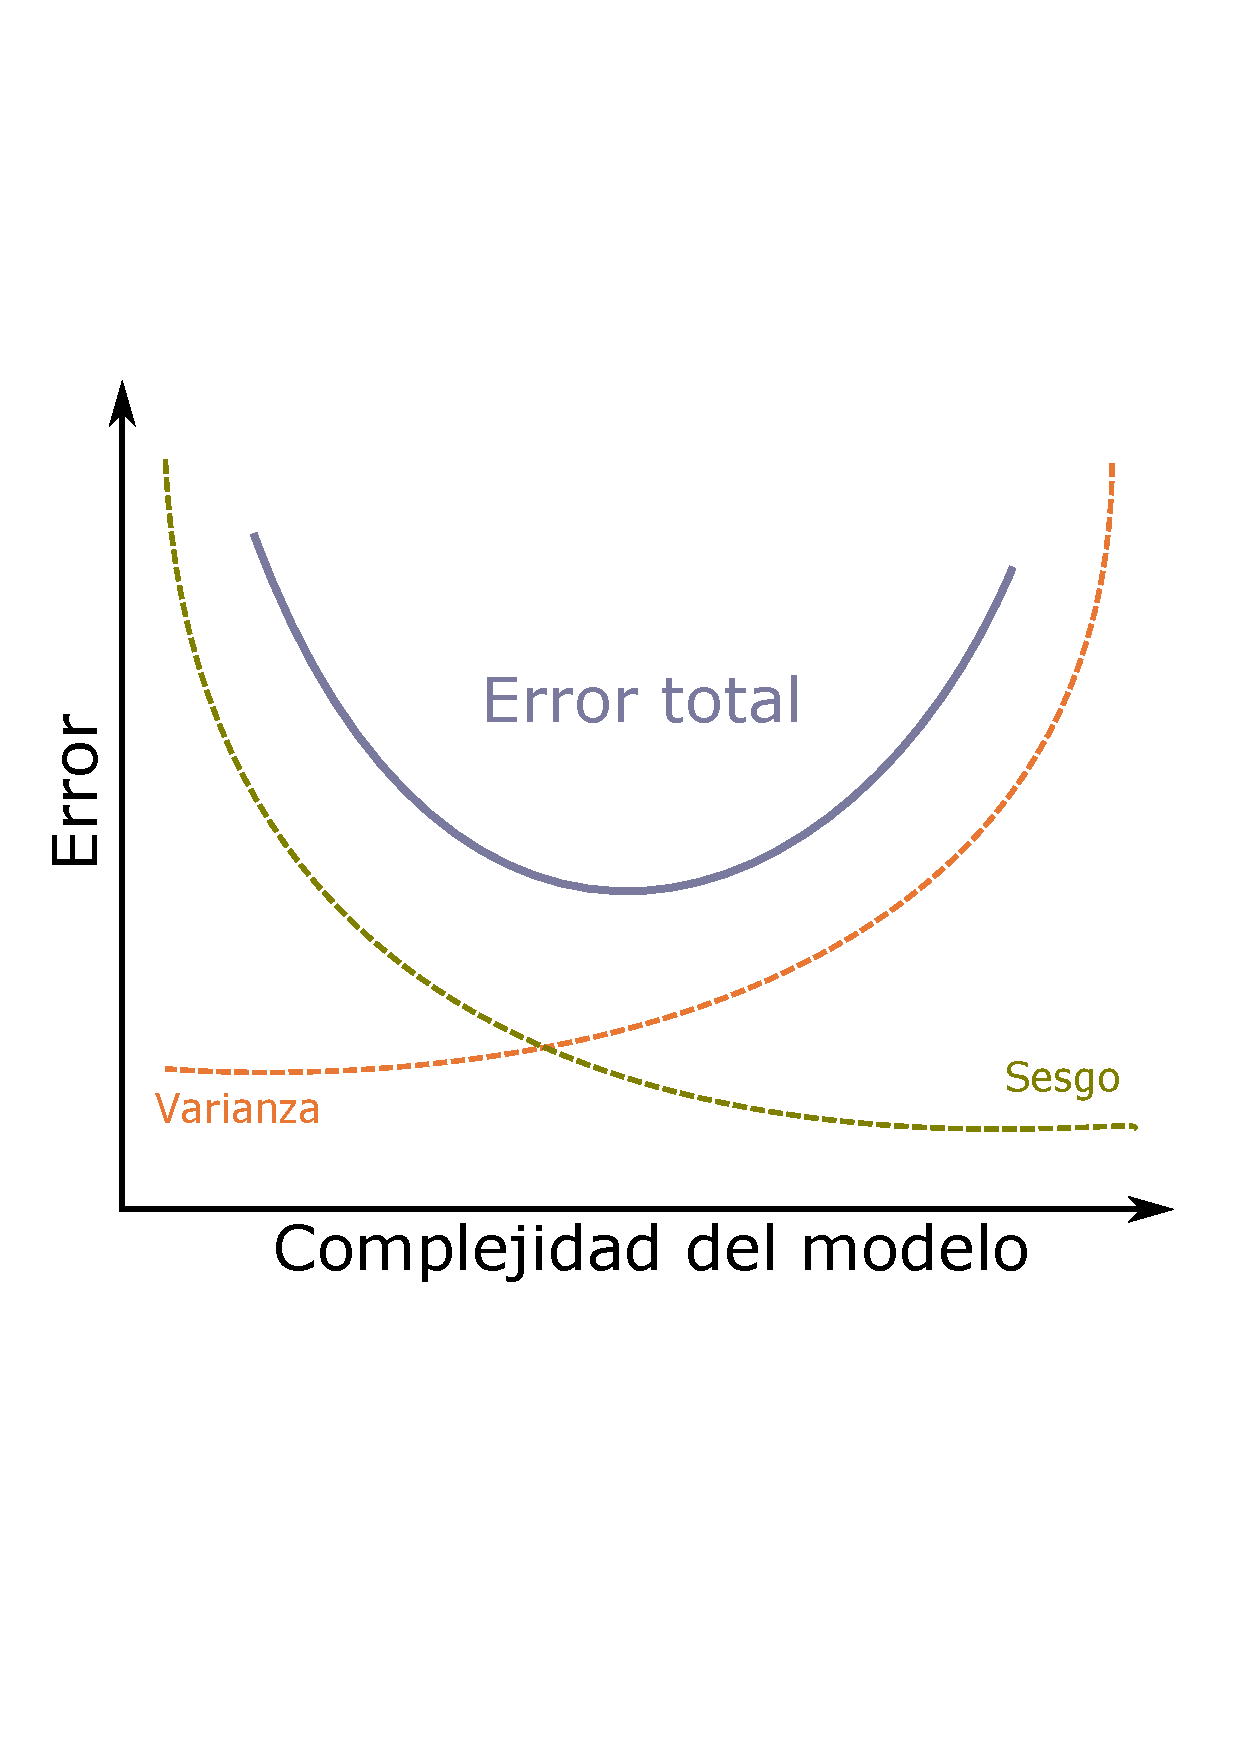
\includegraphics[width = 0.45\linewidth]{img/cap4_biasvariance.pdf}
    \caption{Tradeoff entre el sesgo y la varianza. Se observa que el error total mínimo es alcanzado en un par $(sesgo,varianza)$ específico.} 
\end{figure}


\subsection{Validación cruzada}

Una primera forma de elegir y evaluar un modelo fuera de muestra, consiste en particionar el conjunto de datos $\mathcal{D}$ en dos, donde con el primer conjunto se realizará el entrenamiento y con el segundo se medirá el rendimiento del modelo de acuerdo a algún criterio predefinido (por ejemplo, ECM). Con el fin de evitar posibles sesgos provocados por una partición en específico, la evaluación de desempeño se debe realizar varias veces sobre conjuntos de validación distintos. De esta forma, al promediar los rendimientos de cada partición se obtiene un rendimiento estimado fuera de muestra, lo cual permite finalmente elegir un modelo, quedándose con aquel que reporte el menor error out-sample. Las distintas formas de mezclar y particionar los datos se conocen como validación cruzada.

\subsubsection{Validación cruzada exhaustiva}

En este tipo de validación cruzada, se prueban todas las posibles permutaciones de los datos al particionar el conjunto $\mathcal{D}$. Se tienen 2 técnicas exhaustivas:

\begin{itemize}
	\item \textbf{leave $p$ out (LpOCV):} el conjunto $\mathcal{D}$ se particiona dejando $p$ elementos para validación y los $N-p$ elementos restantes se utilizan para entrenar el modelo. Este entrenamiento y cálculo de desempeño se repite $C_p^N=\frac{N!}{(N-p)!p!}$ veces, pasando por todos los posibles conjuntos de validación de tamaño $p$.
	\item \textbf{leave one out (LOOCV):} corresponde al caso anterior con $p=1$. En este caso cada dato de $\mathcal{D}$ es utilizado como único elemento de validación mientras el resto de los datos se utiliza para entrenar.
\end{itemize}

\subsubsection{Validación cruzada no exhaustiva}

\begin{itemize}
	\item \textbf{$k$-fold:} el conjunto $\mathcal{D}$ es dividido en $k$ grupos de igual tamaño. Luego, uno de esos grupos es utilizado como validador y el resto como entranemiento. Esto se repite $k$ veces de forma de que todos los grupos sean validadores una y solo una vez.
	\item \textbf{Monte Carlo CV:} se realizan particiones binarias aleatorias de $\mathcal{D}$. Se entrena y evalúa usando el par de conjuntos creados en cada partición.
\end{itemize}

\begin{remark}
Una variante de la validación cruzada es dividir el conjunto $\datos$ en 3, donde los primeros dos conjuntos son utilizados para entrenamiento y validación, mientras que el tercero (conocido como test set) es utilizado para obtener una estimación real del desempeño fuera de muestra del modelo elegido a partir de los dos conjuntos anteriores. Esto se realiza ya que al considerar únicamente el desempeño en el conjunto de validación, por lo general se sobreestima el desempeño real fuera de muestra debido a que el modelo fue elegido precisamente tomando el que reporta el menor error dentro del conjunto de validación.\\

Si bien no hay una regla estándar que indique cómo particionar el conjunto, una división usual es utilizar el 50\% para entrenamiento y 25\% para validación y test.
\end{remark}

\subsection{Selección de modelo}

Si bien la técnica de validación cruzada es bastante efectiva, tiene la limitación de requerir una gran cantidad de datos para poder realizar la partición de $\datos$. Para los casos que en los que no se cuenta con una cantidad considerable de observaciones, se requieren herramientas más sofisticadas para poder tomar una decisión acerca de qué modelo elegir. Los dos criterios más usuales corresponden al criterio de información de Akaike y al criterio de información bayesiano.\\

\subsubsection{Criterio de información de Akaike (AIC)}


Sea $\datos=(x_i)_{i=1}^N$ un conjunto de observaciones generadas por una distribución desconocida perteneciente a una familia paramétrica cuyos parámetros están en $\Theta\subset\R^d$. Bajo este modelo, se puede utilizar el estimador de máxima verosimilitud:

\begin{equation}
	\hat{\theta} = \argmax_{\theta\in\Theta} L(\theta|\datos) =  \argmax_{\theta\in\Theta} l(\theta|\datos)
\end{equation}

Una forma de evaluar el desempeño real de este estimador es mediante el \emph{riesgo de predicción}, el cual se ve reflejado en la log-verosimilitud de $\hat{\theta}$ sobre todas las posibles observaciones: $\E(l(\hat{\theta}|x))$. Dado que solo se cuenta con una cantidad finita de muestras, solo es posible obtener un riesgo empírico. El criterio de información de Akaike (AIC) busca ajustar este riesgo para obtener un estimador asintóticamente insesgado del riesgo real. Para esto, se tienen las siguientes definiciones para el estimador de máxima verosimilitud $\hat{\theta}$:

\begin{itemize}
	\item \textbf{Riesgo empírico:} $R_\datos(\hat{\theta})=-\hat{l}$, donde $\hat{l}=l(\hat{\theta}|\datos)$ es la log-verosimilitud del EMV empírico.
	\item \textbf{Riesgo real:} $R(\hat{\theta})=-\E(N\cdot l_0(\hat{\theta}))$, donde $l_0(\theta)=\E(l(\theta|x))$ corresponde a la log-verosimilitud de $\theta$ sobre todo el espacio muestral. Notar que se multiplica por $N$ ya que en el riesgo empírico no se normalizó por $N$.
\end{itemize}

Para poder obtener el $AIC$ se analizará el sesgo asintótico del riesgo empírico con respecto al riesgo real. Para esto, se utilizarán aproximaciones sobre ambos riesgos, asumiendo que a medida que $N$ crece, el EMV empírico tiende al EMV global (por LGN), por lo que el residuo de Taylor tenderá a 0.\\

Sea $\theta_0 = \argmax_{\theta\in\Theta} l_0(\theta)$ el EMV sobre todo el espacio muestral. Utilizando una aproximación de Taylor de segundo orden sobre $l_0$ alrededor de $\theta_0$:
\begin{align}
	l_0(\hat{\theta})&\approx l_0(\theta_0) + (\hat{\theta}-\theta_0)^\top \nabla l_0(\theta_0) + \frac{1}{2}(\hat{\theta}-\theta_0)^\top H_{l_0}(\theta_0) (\hat{\theta}-\theta_0)\\
	&= l_0(\theta_0) + \frac{1}{2}(\hat{\theta}-\theta_0)^\top H_{l_0}(\theta_0) (\hat{\theta}-\theta_0)
\end{align}

Donde se usó que $\nabla l_0(\theta_0)=0$ ya que $\theta_0$ es un punto crítico de $l_0$. De esta forma, se tiene una aproximación de segundo orden para el riesgo real:

\begin{equation*}
	R(\hat{\theta}) \approx -N \cdot l_0(\theta_0) - \frac{N}{2}\E\left((\hat{\theta}-\theta_0)^\top H_{l_0}(\theta_0) (\hat{\theta}-\theta_0)\right)
\end{equation*}

Por otra parte, realizando una expansión de Taylor de segundo orden sobre $\hat{l}$ alrededor de $\theta_0$:
\begin{equation}
	\hat{l} = \sum_{i=1}^N l(\hat{\theta}|x_i) \approx \sum_{i=1}^N l(\theta_0|x_i) + (\hat{\theta}-\theta_0)^\top \sum_{i=1}^N \nabla l(\theta_0|x_i) + \frac{1}{2}(\hat{\theta}-\theta_0)^\top \sum_{i=1}^N H_l(\theta_0|x_i) (\hat{\theta}-\theta_0)
\end{equation}

Usando el hecho de que $\hat{\theta}$ es punto crítico de $l(\cdot|\datos)$:
\begin{equation}
	\sum_{i=1}^N \nabla l(\theta_0|x_i) = \sum_{i=1}^N \nabla \left(l(\theta_0|x_i) - l(\hat{\theta}|x_i)\right) \approx \left(\sum_{i=1}^N \nabla l(\theta_0|x_i)\right) (\theta_0-\hat{\theta}) \approx N \E(H_l(\theta_0|x)) (\theta_0-\hat{\theta})
\end{equation}

Luego, sustituyendo en $\hat{l}$ y notando que $\sum\limits_{i=1}^N H_l(\theta_0|x_i) \approx N\E(H_l(\theta_0|x))$:

\begin{align}
	&\hat{l} \approx \sum_{i=1}^N l(\theta_0|x_i) + N(\hat{\theta}-\theta_0)^\top \E(H_l(\theta_0|x)) (\theta_0-\hat{\theta}) + \frac{N}{2}(\hat{\theta}-\theta_0)^\top \E(H_l(\theta_0|x)) (\hat{\theta}-\theta_0)\\
	&\implies \E(R_\datos(\hat{\theta})) = -Nl_0(\theta_0) + \frac{N}{2} \E\left((\hat{\theta}-\theta_0)^\top H_{l_0}(\theta_0) (\hat{\theta}-\theta_0)\right)
\end{align}

De este modo, el sesgo del riesgo empírico como estimador del riesgo real es:

\begin{equation*}
	\E(R_\datos(\hat{\theta})) - R(\hat{\theta}) = -N \E\left((\hat{\theta}-\theta_0)^\top H_{l_0}(\theta_0) (\hat{\theta}-\theta_0)\right)
\end{equation*}

Por otra parte, dado que $\sqrt{N}\left(\hat{\theta}-\theta_0\right)\approx\mathcal{N}\left(0,H_{l_0}(\theta_0)^{-1}\right)$, la forma cuadrática anterior puede ser aproximada por una distribución de Pearson: $N(\hat{\theta}-\theta_0)^\top H_{l_0}(\theta_0) (\hat{\theta}-\theta_0)\approx\mathcal{X}^2_d$, donde $\E(\mathcal{X}^2_d)=d$. De este modo,

\begin{equation}
	\E(R_\datos(\hat{\theta})) - R(\hat{\theta}) \approx -d
\end{equation}

Por lo que corrigiendo $R_\datos(\hat{\theta})$ se obtiene un estimador asintóticamente insesgado del riesgo real: $R_\datos(\hat{\theta})+d$. De esta forma, se tiene la siguiente definición:

\begin{definition}[AIC]
	Sea $M$ un modelo estadístico $d$-paramétrico y $\datos=(x_i)_{i=1}^N$ un conjunto de observaciones. El AIC del modelo (aproximado por $\datos$) se define como
	
	\begin{equation}
		AIC(M,\datos):=2d-\log\left(\hat{L}(\datos)\right)
	\end{equation}
	
	Donde $\hat{L}(\datos)$ corresponde a la verosimilitud del EMV asociado a $\datos$, es decir:
	
	\begin{equation}
		\hat{L}(\datos) = \prod_{i=1}^N p(x_i|\hat{\theta}),\text{ para } \hat{\theta} = \argmax_{\theta\in\Theta} L(\theta|\datos)
	\end{equation}
\end{definition}

\begin{remark}
El AIC corresponde al estimador asintóticamente insesgado del riesgo real multiplicado por 2. Esta ponderación es realizada por motivos históricos (Model selection and multimodel inference, Burnham \& Anderson).
\end{remark}

De acuerdo a la derivación anterior, el AIC es una medida relativa de la pérdida de información de un modelo de acuerdo a un conjunto de entrenamiento $\datos$. De esta forma, para un conjunto de posibles modelos, se debe elegir el modelo que presente el menor valor AIC ya que será el que minimice el riesgo de predicción.\\

Como se puede ver en la definición, el criterio de Akaike no se basa únicamente en la verosimilitud del modelo sino que agrega una penalización de acuerdo a la cantidad de parámetros, evitando elegir un modelo sobreajustado a los datos. 

\begin{remark}
	Una de las hipótesis de AIC es que el espacio muestral es infinito ya que se asume que el error de Taylor es despreciable. Para una cantidad finita de datos, se puede realizar una corrección del estimador dada por:
	
	\begin{equation}
		AICc(M,\datos) := AIC(M,\datos) + \frac{2d(d+1)}{N-d-1}
	\end{equation}
	
	Es importante notar que cuando $N\to\infty$ se recupera el AIC original.
\end{remark}

\subsubsection{Criterio de información bayesiano (BIC)}

Otro enfoque para la selección de modelos corresponde al criterio de información bayesiano (o criterio de Schwarz). Dada una familia de modelos $\mathcal{M}$, se define un prior $p(m)$ para cada modelo $m\in\mathcal{M}$. Además, se define un prior $p(\theta|m)$ sobre los parámetros de cada modelo. El criterio de información bayesiano (BIC) elige al mejor modelo de acuerdo a la posterior $p(m|\datos)$, la cual viene dada de acuerdo al teorema de Bayes:

\begin{equation}
	p(m|\datos)=\frac{p(\datos|m)p(m)}{p(\datos)}\propto p(\datos|m)p(m)
\end{equation}

De forma similar al criterio de Akaike, se puede calcular la verosimilitud del modelo $p(\datos|m)$ mediante aproximaciones de Taylor, probando que es independiente del prior. La derivación de $p(\datos|m)$ lleva a la siguiente definición:

\begin{definition}[BIC]
	Sea $M$ un modelo estadístico $d$-paramétrico y $\datos=(x_i)_{i=1}^N$ un conjunto de observaciones. El BIC del modelo (aproximado por $\datos$) se define como
	
	\begin{equation}
		BIC(M,\datos):= d\cdot\log(N) - 2\log\left(\hat{L}(\datos)\right)
	\end{equation}
	
	Donde nuevamente $\hat{L}(\datos)$ corresponde a la verosimilitud del EMV asociado a $\datos$.
\end{definition}

En este caso, se vuelve a elegir el modelo que presente el menor BIC. Se observa que, al igual que AIC, BIC contiene una penalización sobre el número de parámetros por lo que también evita el sobreajuste a los datos.

\begin{remark}[Stone (1977) - Shao (1997)] Para una familia de modelos, minimizar el AIC es asintóticamente equivalente a realizar LOOCV. Por otra parte, minimizar el BIC es asintóticamente equivalente a realizar leave $p$ out cross validation para

\begin{equation}
	p=\left\lfloor N\left(1-\frac{1}{\log(N)-1}\right)\right\rfloor
\end{equation}
	
\end{remark}

\begin{mdframed}[style=pendiente, frametitle={\center AIC y BIC para la regresión lineal}]

Al igual que en máxima verosimilitud, se puede considerar un modelo generativo para la regresión lineal de la forma $ y = c^\top x + \epsilon$, donde $\epsilon\sim\cN(0,\sigma^2)$ y por lo tanto, $y|x \sim \cN(y;c^\top x,\sigma^2)$. Sean $\hat{c}$ y $\hat{\sigma}^2$ los EMV del modelo (calculados en el capítulo de regresión), entonces la log-verosimilitud máxima viene dada por:
\begin{align}
	\hat{l}(\datos) &= \frac{-N}{2}\log(2\pi\hat{\sigma}^2) - \frac{1}{2\hat{\sigma}^2} \sum_{i=1}^N( y_i-\hat{c}^\top x_i)= -\frac{N}{2}\log(2\pi) - \frac{N}{2}\log(\hat{\sigma}^2) - \frac{1}{2\hat{\sigma}^2}  N\hat{\sigma}^2\\
	&= C(N) - \frac{N}{2}\log(\hat{\sigma}^2) = C(N)- \frac{N}{2}\log\left(\frac{1}{N}\text{RSS}(\datos)\right)
\end{align}	

Donde $C(N) = -\frac{N}{2}\log(2\pi) - N$ y $\text{RSS}(\datos)$ corresponde a la suma de cuadrados residuales: $\text{RSS}(\datos) := \sum_{i=1}^N \left(y_i - c^\top x_i\right)^2$. Dado que $C(N)$ es una constante independiente del modelo, puede ser omitida en la comparación de modelos, por lo tanto:

\begin{itemize}
	\item $AIC=2d-N\log(\frac{1}{N}\text{RSS}(\datos))$
	\item $BIC = d\log(N) - N\log(\frac{1}{N}\text{RSS}(\datos))$
\end{itemize}

\end{mdframed}

Si bien existen otros métodos de selección de modelo (DIC, WAIC, entre otros), estos tienen una formulación más compleja que se escapa del alcance de este curso ya que se requieren herramientas adicionales como MCMC para el cálculo de distribuciones posteriores.

\subsection{Evaluación de modelos}
Una vez elegido el mejor modelo de acuerdo a un criterio establecido (AIC o BIC), es deseable poder conocer el desempeño de dicho modelo. Existen varias formas de evaluar un modelo, una de ella podría ser simplemente evaluar la precisión de sus predicciones. A veces es natural fijarse en la precisión, como en los problemas de pronóstico. Otras veces la precisión es importante para evaluar diferentes modelos y elegir uno de ellos. En esta sección presentaremos dos maneras distintas de evaluar modelos, cada forma sirve en distintos escenarios, los cuales se discutirán a través de la predicción puntal, que resume la predicción de un conjunto de datos en una solo valor.

\subsubsection{Error cuadrático medio}

El ajuste del modelo a nuevos datos se puede resumir en una predicción puntual llamada error cuadrático medio, el cual está definido por:

\begin{equation}
MSE(\theta) = \frac{1}{n}\sum_{i=1}^N (y_i-\mathbb{E}(y_i|\theta))^2
\end{equation}

o su versión ponderada:

\begin{equation}
MSE(\theta) = \frac{1}{n}\sum_{i=1}^N \frac{(y_i-\mathbb{E}(y_i|\theta))^2}{\mathbb{V}\text{ar}(y_i|\theta)}
\end{equation}

Esta forma de medir el error tiene la ventaja de ser fácilmente computable e interpretable, pero no es apropiada para modelos que están lejos de la distribución normal.

\subsubsection{log-densidad predictiva o log-verosimilitud}
Otra forma de realizar esta evaluación es utilizando el estadístico \emph{log-densidad preditiva} $\log p(y|\theta)$ el cual es proporcional a error cuadrático medio si el modelo es normal con varianza constante. Estudiaremos el caso de un solo punto, para luego extrapolar a más de un punto.\\

\textbf{Predictive accuracy para un punto:} sea $f$ el modelo real, $y$ las observaciones (es decir, una realización del dataset $y$ de la distribución $f(y)$), y llamaremos $\tilde{y}$ a la data futura o un dataset alternativos que podemos ver. El ajuste predictivo out-of-sample para un nuevo punto $\tilde{y}_i$ está dado por:

\begin{equation}
\log p_{\text{post}}(\tilde{y}_i) = \log \mathbb{E}[p(\tilde{y}_i|\theta)] = \log \int p(\tilde{y}_i|\theta)p_{\text{post}}(\theta)d\theta
\end{equation}

\textbf{Promedio de las distribuciones para un punto:} al tener un dato nuevo $\tilde{y}_i$ entonces se puede calcular el la log-densidad predictiva (elpd, por su sigla en inglés) para el nuevo punto:
\begin{align}
\notag \text{elpd} & = \mathbb{E}_f[\log p_{\text{post}}(\tilde{y}_i)]\\
& = \int \log p_{\text{post}}(\tilde{y}_i) f(\tilde{y}_i)d\tilde{y}
\end{align}

\textbf{Promedio de las distribuciones para datasets futuros:} como usualmente, no se tiene solo un punto, se debe realizar la suma sobre el conjunto de puntos, calculando así la log-densidad predicitiva puntual (elppd, por su sigla en inglés).

\begin{align}
\text{elppd} & = \sum_{i=1}^N \mathbb{E}_f[\log p_{\text{post}}(\tilde{y}_i)]
\end{align}

En la práctica, como siempre se tiene la distribución de todos los modelos y la expresión anterior requiere de esto, se suele calcular el estadístico sobre una estimación de un modelo $\hat{\theta}$ (como por ejemplo, el máximo de la función de verosimilitud):

\begin{align}
\text{elppd}|\hat{\theta} & = \sum_{i=1}^N \mathbb{E}_f[\log p_{\text{post}}(\tilde{y}_i|\hat{\theta})]
\end{align}

Finalmente, una última extensión de este estadístico es cuando se puede tener \emph{draws} de la posterior, es decir, tenemos $\{ \theta^s\}_{s=1}^S$, entonces el lppd computado es:

\begin{equation}
\text{computed lppd} = \sum_{i=1}^N \left( \frac{1}{S} \sum_{s=1}^S p(y_i|\theta^s)\right)
\end{equation}


\subsection{Promedio de modelos}
Hay veces que no queremos elegir un solo modelo, puesto que quizás nos interesan las estimaciones de dos o más modelos. Para estos casos, se puede utilizar la técnica de \emph{model averaging}, la cual consiste en utilizar una combinación lineal de distintos modelos.\\

Sea $\mathcal{M}$ un conjunto de modelos donde cada modelo $m\in\mathcal{M}$ tiene asociada una distribución $\mu_m$ sobre el espacio muestral. Un promedio de modelos $\hat{\mu}$ es una combinación convexa de los modelos de $\mathcal{M}$, es decir:

\begin{equation}
\hat{\mu} = \sum_{m\in \mathcal{M}} c(m) \mu_m
\end{equation}

Donde los pesos $\left(c(m)\right)_{m\in\mathcal{M}}\subset\R_+$ cumplen que $\sum_{m\in \mathcal{M}} c(m) = 1$.\\

La principal dificultad para elegir los pesos, está en que se debe asegurar que la suma de los pesos sea unitaria y que estos sean todos positivos. Una forma de asegurar esto es aplicar una función $f$ positiva sobre una función $g$ (\emph{score}) que evalúe el modelo, de modo que:

\begin{equation}
\sum_{m\in \mathcal{M}} (f\circ g)(m) > 0
\end{equation}

De esta forma, se pueden definir los pesos mediante normalización:

\begin{equation}
c(s) = \frac{(f\circ g)(s)}{\sum_{m\in \mathcal{M}} (f\circ g)(m)}
\end{equation}

Para la función $g$ se pueden utilizar los criterios AIC o BIC ya que entregan una evaluación del desempeño relativo del modelo. Por otra parte, usando $f(x)=\exp(x)$ los pesos $\left(c(m)\right)_{m\in\mathcal{M}}$ vienen dados por la función softmax:



\begin{align}
c_{AIC}(s) = \frac{\exp\{ \frac{1}{2} \text{AIC}(s)\}}{\sum_{m\in \mathcal{M}} \exp\{ \frac{1}{2} \text{AIC}(m)\}} & & c_{BIC}(s) = \frac{\exp\{ \frac{1}{2} \text{BIC}(s)\}}{\sum_{m\in \mathcal{M}} \exp\{ \frac{1}{2} \text{BIC}(m)\}}
\end{align}

%!TEX root = ../notas_de_clase.tex

\newpage
\section{Redes Neuronales}

\subsection{Introducción y arquitectura}

\subsubsection{Conceptos básicos}

Los modelos escenciales de redes neuronales se conocen como \textbf{feedforward neural networks}, o \textbf{multilayer perceptrons} (MLPs). Una red neuronal busca aproximar una funci\'on $f^*$. Una red feedforward define un mapping $\bm{y}=f(\bm{x}; \bm{\theta})$ y aprende los par\'ametros $\bm{\theta}$ que resultan en la mejor aproximaci\'on posible.

Estos modelos se conocen como redes ya que que t\'ipicamente son el resultado de composiciones sucesivas de varios tipos de funciones. Por ejemplo, sean $f^{(1)}$, $f^{(2)}$ y $f^{(3)}$ funciones, estas se 'conectan' para formar $f(\bm{x}) = f^{(3)}(f^{(2)}(f^{(1)}(\bm{x})))$, se dice que $f^{(1)}$ es la primera \textbf{capa} de la red, $f^{(2)}$ la segunda y $f^{(3)}$ la tercera. El largo de esta cadena define la \textbf{profundidad} de la red. El uso de redes neuronales con m\'ultiples capas se conoce como \textbf{deep learning}, aunque este t\'ermino se usa para problemas m\'as espec\'ificos de aprendizaje de m\'aquinas usando redes neuronales profundas (ver secci\'on 3.5).

Durante el entrenamiento de una red neuronal se busca que $f(\bm{x}) \approx f^*(\bm{x})$, donde la data de entrenamiento provee aproximaciones ruidosas de $f^*(\bm{x})$. Cada dato $\bm{x}$ viene acompa{\~{n}}ado de una etiqueta, $y \approx f^*(\bm{x})$. Los datos de entrenamiento indica qu\'e debe reproducir la red en su \'ultima capa, lo cual debe ser un valor aproximado de $y$. El comportamiento del resto de las capas no tiene una interpretación tan directa como la última capa, por lo que el algoritmo de aprendizaje debe decidir c\'omo adaptar las capas para que el output producido por la red sea lo m\'as cercano posible a $y$, la etiqueta, para cada punto $\bm{x}$. Es por esto que estas capas intermedias se denominan \textbf{capas ocultas}.

Estas redes se llaman \textit{neuronales} por su inspiraci\'on neurocient\'ifica. Cada capa oculta de la red corresponde a un vector. Se podr\'ia pensar que cada elemento de estos vectores tiene un rol similar al de una neurona, en vez de pensar cada capa como una funci\'on que produce un mapping de vector a vector, podr\'ia considerarse que una capa consiste en muchas \textbf{unidades} que act\'uan en paralelo, cada una representando un mapping de vector a escalar. La elecci\'on de las funciones $f^{(i)}(\bm{x})$, conocidas como \textbf{funciones de activaci\'on}, en varios casos ha sido guiada por observaciones sobre el comportamiento de neuronas biol\'ogicas.

\begin{figure}[H]
\captionsetup{font=small,labelfont=small}
\caption{Ejemplo de una red neuronal de 1 capa: (\textit{izquierda}) Se muestra la red con inputs $x_1$ y $x_2$, que luego pasan a la capa oculta para producir el output $y$. (\textit{derecha}) Misma red con una representaci\'on vectorial de las capas. La matriz ${\bm{W}}$ describe el mapping de ${\bm{x}}$ a ${\bm{h}}$, y la matriz $w$ el mapping de ${\bm{h}}$ a $y$.}
\centering
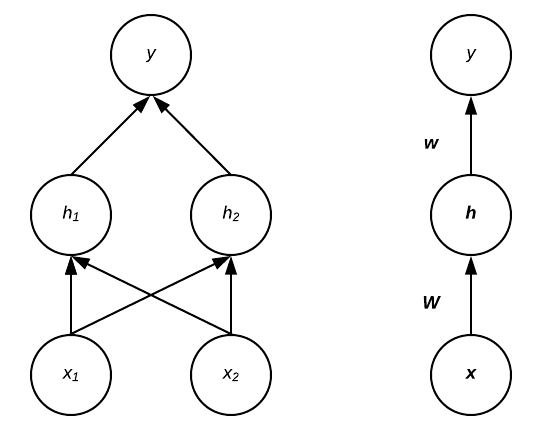
\includegraphics[scale=.5]{img/cap7_F1NN1L.png}
\end{figure}

Como se puede apreciar en la figura, los coeficientes ${\bm{W}}$ y $w$ se usan para producir el output para la siguiente capa (denominados \textbf{pesos}), por lo que la primera operaci\'on de esta red ser\'a entregar $h_{1}$ y $h_{2}$ mediante la transformaci\'on ${\bm{W}^{T}}\bm{x} + \bm{b}^{(1)}$. Luego, esta red aplica $w^{T} \boldsymbol{h} + b^{(2)}$ para producir el output $y$. Los coeficientes $\bm{b}^{(1)}$ y  $b^{(2)}$ se conocen como t\'erminos de \textbf{bias} (sesgo). Todos los parámetros de la red neuronal, los pesos y \textit{bias}, serán agrupados en el t\'ermino $\bm{\theta}$.

\subsubsection{Funci\'on de costos, unidades de output y la formulaci\'on como un problema probabil\'istico}

Una de las principales diferencias entre los modelos lineales antes vistos y una red neuronal, es que el uso de ciertas funciones de activaci\'on hacen que la funci\'on de costos no sea convexa, esto hace que el entrenamiento realizado en base a descenso de gradiente no entregue garant\'ias de que se alcanzar\'a el \'optimo global, o una buena solución en términos generales, ya que el algoritmo podría estancarse en un optimo local que entregue resultados pobres. 

En la mayor\'ia de los casos, el modelo param\'etrico define una distribuci\'on $p(y|\bm{x}; \bm{\theta})$, por lo que los par\'ametros del modelo se estimar\'an usando m\'axima verosimilitud, as\'i, se optimizar\'a la log-verosimilitud negativa, es decir, la \textbf{funci\'on de costos} a usar ser\'a la \textbf{cross-entropy}:

\begin{equation}
J(\bm{\theta}) = -\E_{\bm{x},\bm{y}\sim \hat{p}_{\textrm{data}}}(\textrm{log}\; p_{\textrm{modelo}}(\bm{y}|\bm{x}))
\end{equation}

De esta forma la elecci\'on de la \textbf{unidad de output} definir\'a la forma que toma la funci\'on de costos, pero no ser\'a necesario definir una funci\'on especifica para cada problema; en general siempre se resolver\'a el problema por m\'axima verosimilitud. La elecci\'on en la unidad de output depender\'a del tipo de problema que se quiera resolver. Cuando se quiera retornar la media de una distribuci\'on Gaussiana condicional, $p(\bm{y}|\bm{x}) = \mathcal{N}(\bm{y}|\hat{\bm{y}};\bm{I})$, la unidad de output deber\'a ser un modelo lineal, $\hat{\bm{y}} = \bm{W}^{T}\bm{h} + \bm{b}$, en donde $\bm{h}$ es el output de la red que proviene de todas las capas ocultas anteriores. En este caso, maximizar la log-verosimilitud es equivalente a minimizar el error cuadr\'atico medio, por esta razón este tipo de output es adecuada para un problema de regresión.

Cuando el problema objetivo es clasificaci\'on binaria, una unidad de output apropiada es la funci\'on sigmoidal. Para resolver el problema de m\'axima verosimilitud, se modela utilizando una distribuci\'on Bernoulli en $y$ condicional en $\bm{x}$. Una unidad de output sigmoidal se define como $\hat{{y}} = \sigma(\bm{w}^{T}\bm{h} + {b})$. Esto entrega como output $P(y=1|\bm{x})$, por lo que se podr\'a decidir a qu\'e clase pertenece $y$ basado en el output de la red, esto se interpreta como la probabilidad de que la observaci\'on sea de la clase 1.

Para un problema de clasificaci\'on multiclase, la unidad de output apropiada es la generalizaci\'on de la funci\'on sigmoidal, conocida como softmax. El problema es predecir a cu\'al de $n$ clases pertenece $y$, por lo que se requiere producir un vector $\hat{\bm{y}}$, con $\hat{y_{i}} = P(y=i|\bm{x})$, por lo que se usar\'a una distribuci\'on multinoulli. Primero, una capa lineal predice las log-probabilidades no normalizadas, $\bm{z} = \bm{W}^{T}\bm{h} + \bm{b}$, y luego se aplica la funci\'on softmax para obtener los valores de $\hat{\bm{y}}$ antes descritos:

\begin{equation}
\textrm{log softmax}(\bm{z})_{i} = \textrm{log}\frac{\textrm{exp}(z_{i})}{\sum_{j=1}^{n}\textrm{exp}({z_{j}})} = z_{i} - \textrm{log}\sum_{j=1}^{n}\textrm{exp}({z_{j}})
\end{equation}

\subsubsection{Estructura interna de la red}

Las capas escondidas proveen a la red neuronal la flexibilidad necesaria para aprender funciones extremadamente complejas, esto mediante el uso de activaciones no lineales. En varios casos estas funciones son incluso no diferenciables, lo que llevar\'ia a pensar de que no son v\'alidas para ser usadas en conjunto con algoritmos que usan descenso de gradiente, pero en la pr\'actica tienen un desempe\~{n}o suficientemente bueno para ser usadas en tareas de aprendizaje de m\'aquinas. En general, las funciones de activaci\'on para las unidades escondidas toman como input un vector $\bm{x}$ para el cual obtienen una transformaci\'on af\'in $\bm{z} = \bm{W}^{T}\bm{x} + \bm{b}$, para luego aplicar una transformaci\'on no lineal $g(\bm{z})$. Las unidades escondidas m\'as comunes son las \textbf{rectified linear units} o \textbf{ReLUs}, $g(\bm{z}) = \textrm{max}(0, \bm{z})$, y sus generalizaciones como \textbf{leaky ReLU}, $g(\bm{z})_{i} = \textrm{max}(0, \bm{z}_{i}) + \alpha_{i}\textrm{min}(0, \bm{z}_{i})$, con $\alpha_{i}$ una constante peque\~{n}a como 0.01; la funci\'on sigmoidal $g(\bm{z}) = \sigma(\bm{z})$; y la tangente hiperb\'olica $g(\bm{z}) =  \textrm{tanh}(\bm{z}) = 2\sigma(2\bm{z}) - 1$. A diferencia de las funciones lineales por partes, las unidades sigmoidales se saturan en la mayor parte de su dominio (su gradiente se aproxima a 0) haciendo imposible el aprendizaje por el gradiente cuando esto ocurre, por lo que su uso como unidades escondidas ha sido desalentado.

\subsubsection{Dise\~{n}o de arquitectura y teorema de aproximaci\'on universal}

La \textbf{arquitectura} de una red neuronal se refiere a la totalidad de su estructura: la cantidad de capas, la cantidad de unidades escondidas, la conexi\'on entre las unidades, etc. Bajo la estructura mostrada para una red feedforward, la primera capa y la segunda capa son de la forma:

\begin{equation}
\begin{split}
\bm{h}^{(1)} = g^{(1)}(\bm{W}^{(1) T}\bm{x} + \bm{b}^{(1)}) \\
\bm{h}^{(2)} = g^{(1)}(\bm{W}^{(2) T}\bm{h}^{(1)} + \bm{b}^{(2)})
\end{split}
\end{equation}

En una arquitectura de este tipo, la principal consideraci\'on respecto al dise\~{n}o es la profundidad y ancho (cantidad de unidades por capa) de cada capa. Una red con solo 1 capa escondida puede ser suficiente para ajustar el set de entrenamiento, cabe destacar que la cantidad de neuronas necesarias en esta única capa podría ser muy grande y la capacidad de generalización puede ser baja, dependiendo de la complejidad de los datos con los que se pretende trabajar. Redes m\'as profundas generalmente permiten disminuir el n\'umero de unidades por capa (de esta forma tener una menor cantidad par\'ametros en total), como as\'i tambi\'en una mejor capacidad de generalización en el set de testeo, con esto se hace referencia a la capacidad de la red para clasificar correctamente ejemplos que no fueron usados para el proceso de entrenamiento, naturalmente hacer más intrincado el diseño de la red hará que el proceso de optimización para ajustar los parámetros sea más costoso. La arquitectura ideal se debe encontrar por experimentaci\'on con distintas estructuras acompañado de conocimiento sobre el tipo de datos, esto se apoya mediante el monitoreo del error en el set de validaci\'on.

Una de las principales justificaciones para usar redes neuronales se debe al \textbf{Teorema de Aproximaci\'on Universal} (Horniket al., 1989; Cybenko, 1989), el cual muestra que una red feedforward con una capa de output lineal y al menos una capa escondida con funci\'on de activaci\'on sigmoidal (y otras similares) puede aproximar cualquier funci\'on Borel medible \footnote{En particular cualquier funci\'on continua en un subconjunto cerrado y acotado de $\R^{n}$ es Borel medible, la clase de funciones Borel medibles es mucho más rica y variada que las funciones continuas.} de un espacio dimensión finita a otro, con un nivel de error arbitrariamente pequeño, provisto de que hayan suficientes unidades escondidas. Una red neuronal tambi\'en puede aproximar un mapping de cualquier espacio dimensional finito y discreto a otro, y este teorema tambi\'en se ha probado para una amplia gama de funciones de activaci\'on, como para la m\'as com\'unmente usada ReLU (Leshno et al., 1993). La desventaja del teorema es que a pesar que asegura que la red podr\'a aproximar cualquiera de estas funciones, esto no implica que necesariamente podr\'a \textit{aprender} la funci\'on en sí. Una razón posible es que el algoritmo de optimizaci\'on podr\'ia no encontrar los par\'ametros de la red que alcancen el nivel de error deseado. Tampoco especifica la cantidad de unidades que son necesarias para alcanzar un nivel de error dado, lo cual podr\'ia ser excesivamente grande. Sin embargo en muchos casos modelos m\'as profundos necesitar\'an menos unidades y potencialmente permiten reducir el error de generalizaci\'on.

\subsection{Entrenamiento de una red neuronal}

\subsubsection{Forward propagation y back-propagation}

Al usar una red neuronal feedforward, la informaci\'on fluye a trav\'es de la red desde el ingreso de un input $\bm{x}$ hasta producir un output $\hat{\bm{y}}$. Esto se conoce como \textbf{forward propagation}. Durante el entrenamiento, \textit{forward propagation} contin\'ua hasta producir el costo escalar $J(\bm{\theta})$.

El algoritmo de \textbf{back-propagation} permite que la informaci\'on del costo fluya en sentido inverso a trav\'es de la red para calcular el gradiente de manera computacionalmente eficiente. El gradiente se calculará de esta forma ya que, aunque es posible obtener una expresi\'on anal\'itica para este, evaluar la expresi\'on puede ser muy caro computacionalmente. Luego de obtener el gradiente, otro algoritmo como descenso de gradiente estoc\'astico (ver secci\'on 4) realiza el aprendizaje usando la expresión que fue calculada. En algoritmos de aprendizaje el gradiente que m\'as com\'unmente se requiere obtener es $\nabla_{\bm{\theta}}J(\bm{\theta})$, aunque el algoritmo de \textit{back-propagation} no se limita a esto y puede ser usando para otras tareas que involucren obtener derivadas.

Sea $\bm{x} \in \R^{m}, \bm{y} \in \R^{n}, g:\R^{m} \rightarrow \R^{n}, f:\R^{n} \rightarrow \R, \bm{y} = g(\bm{x})$ y $z = f(\bm{y})$, la regla de la cadena indica que:

\begin{equation}
\frac{\partial z}{\partial x_{i}} = \sum_{j}\frac{\partial z}{\partial y_{j}}\frac{\partial y_{j}}{\partial x_{i}}
\end{equation}

O de manera equivalente visto en su forma vectorial:

\begin{equation}
\nabla_{\bm{x}}z = (\frac{\partial \bm{y}}{\partial \bm{x}})^{T}\nabla_{\bm{y}}z
\end{equation}

en donde $\frac{\partial \bm{y}}{\partial \bm{x}}$ es la matriz Jacobiana de $g$, con esto se puede ver que para obtener el gradiente con respecto a la variable $\bm{x}$, basta multiplicar la matriz Jacobiana por el gradiente con respecto a $\bm{y}$.% El algoritmo de \textit{back-propagation} consiste en realizar este tipo de operaciones iterativamente, calculando la regla de la cadena con un orden espec\'ifico de operaciones que lo hace altamente eficiente.


Usualmente se aplicar\'a \textit{back-propagation} a \textbf{tensores} de dimensionalidad arbitraria, no solo vectores. Se denota entonces el gradiente de $z$ con respecto a un tensor $\textrm{\textbf{X}}$ como $\nabla_{\textrm{\textbf{X}}}z$. Sean $\textrm{\textbf{Y}} = g(\textrm{\textbf{X}})$ y $z = f(\textrm{\textbf{Y}})$, entonces la regla de la cadena se escribe como:

\begin{equation}
\nabla_{\textrm{\textbf{X}}}z = \sum_{j}(\nabla_{\textrm{\textbf{X}}}\textrm{Y}_{j})\frac{\partial z}{\partial \textrm{Y}_{j}}
\end{equation}

%\newpage
%[AGREGAR DESCRIPCIÓN DE BACK-PROPAGATION]

Antes de proseguir a revisar los algoritmos de \textit{forward-propagation} y \textit{back-propagation} se realizará una breve deducción de \textit{back-propagation} que permitirá comprender de mejor manera el proceso de entrenamiento en una red neuronal, en primer lugar de analizará una red neuronal con solo una capa escondida, luego veremos que esto puede ser extendido de forma fácil a arquitecturas más complejas (osea, más capas).

Sea $\{ (x_i,y_i) \}_{i=1}^N$ un conjunto de puntos sobre los que se quiere ajustar los pesos de una red neuronal, el conjunto de entrenamiento es tal que  $x_i \in \R^p, y_i \in \R^K \quad \forall i=1,...,N$, el problema planteado corresponde a uno de clasificación sobre $K$ clases distintas. Adicionalmente se tiene que el error (función de perdida) puede ser escrito como:

\begin{equation}
J(\theta) = \sum_{i=1}^N J_i = \sum_{i=1}^N L(y_i, f(x_i;\theta))
\end{equation}

Donde $J_i$ corresponde a la discrepancia entre $y_i$ y el valor entregado por la red $f(x_i;\theta)$ evaluado por la función de perdida $L$. Para fijar ideas, la arquitectura de la red está compuesta por $p$ unidades de entrada, la capa escondida tiene $M$ neuronas con funciones de activación sigmoides ($\sigma(x)=\frac{1}{1-e^{-t}}$) y la capa de salida (output) tendrá $K$ unidades y una función de salida $g$. De esta forma el problema puede ser planteado como:

\begin{align}
	Z_m &= \sigma(\alpha_{0m} + \alpha_{m}^TX), \quad \forall m=1,...,M\\
	N_k &= \beta_{0k} + \beta_k^TZ, \quad\quad\quad \forall k=1,...,K\\
	O_k &= g_k(N), \quad\quad\quad\quad \forall k=1,...,K\\
	f(X) &= O\\
\end{align}

Donde $Z=(Z_1,...,Z_M)$, $N=(N_1,...,N_K)$, $O=(O_1,...,O_K)$ y se puede ver que $g:\R^K \rightarrow \R^K$, de esta forma los parámetros $\theta$ del modelo son:

\begin{align}
\{\alpha_{0m}, \alpha_m; \quad m &= 1,...,M \} \quad M(p+1) \quad \text{pesos}\\
\{\beta_{0k}, \beta_k; \quad k &= 1,...,K \} \quad K(M+1) \quad \text{pesos}\\
\end{align}

De ahora en adelante $J\equiv J(\theta)$, también es importante distinguir que es distinto calcular la derivada de $J$ respecto a un peso que está en la capa de salida y un peso que pertenece a una capa escondida, siendo el primer caso mucho más fácil de calcular, esto se justifica por el hecho que los valores de la capa de salida participan directamente en el calculo del error $J$, mientras que los valores de las neuronas escondidas no, esto se hará evidente en los cálculos. Como último preámbulo se definen las siguientes variables que nos ayudaran a hacer los cálculos más claros:

\begin{align}
z_{mi} &= \sigma(\alpha_{0m} + \alpha_{m}^Tx_i)\\
z_i &= (z_{1i},...,z_{Mi})\\
n_{ki} &= \beta_{0k} + \beta_k^Tz_i\\
n_i &= (n_{1i},...,n_{Ki})\\
o_{i} &= g(n_i)\\
o_{ki} &= (o_i)_k\\
\end{align}

Considerando que derivar es una operación lineal calcularemos la derivada de $J_i$, a partir de este termino podemos obtener la derivada de $J$ sumando sobre todo $i=1,...,N$.

\begin{align}
\frac{\partial J_i}{\partial \beta_{km}}&=
\frac{\partial J_i}{\partial o_{ki}}
\frac{\partial o_{ki}}{\partial n_{ki}}
\frac{\partial n_{ki}}{\partial \beta_{km}}\\
&= \frac{\partial J_i}{\partial o_{ki}}
g'_k(n_{ki})z_{mi}
\label{BP_beta}
\end{align}

Dado que $o_{ki}$ pertenece a la capa de salida, esto implica que participa directamente en la expresión de $J_i$ y por lo tanto la derivada $\frac{\partial J_i}{\partial o_{ki}}$ puede ser calculada directamente. El calculo recién hecho se conoce como regla delta ('delta rule') y es el paso principal de \textit{back-propagation}, este consiste en usar la regla de la cadena 2 veces sucesivamente.

Como se mencionó con anterioridad calcular la derivada de $J_i$ respecto a un peso perteneciente a una capa escondida es más engorroso, ya que las neuronas en las capas intermedias no participan directamente en el error, aún así es posible y el calculo entrega una formula recursiva que permite llegar a una expresión cerrada y explicita.

\begin{align}
\frac{\partial J_i}{\partial \alpha_{ml}}&=
\frac{\partial J_i}{\partial z_{mi}}
\frac{\partial z_{mi}}{\partial \alpha_{ml}}\\
&= \left [ \sum_{k=1}^K
\frac{\partial J_i}{\partial o_{ki}}
\frac{\partial o_{ki}}{\partial n_{ki}}
\frac{\partial n_{ki}}{\partial z_{mi}}
\right ]
\frac{\partial z_{mi}}{\partial \alpha_{ml}}\\
&= \left [ \sum_{k=1}^K
\frac{\partial J_i}{\partial o_{ki}}
\frac{\partial o_{ki}}{\partial n_{ki}}
\frac{\partial n_{ki}}{\partial z_{mi}}
\right ]\sigma'(\alpha_0+\alpha_mx_i)x_{il}\\
&= \left [ \sum_{k=1}^K
\frac{\partial J_i}{\partial o_{ki}}
g'(n_{ki})
\beta_{km}
\right ]\sigma'(\alpha_0+\alpha_mx_i)x_{il}\\
&=  \sum_{k=1}^K
\frac{\partial J_i}{\partial o_{ki}}
g'(n_{ki})
\beta_{km}
\sigma'(\alpha_0+\alpha_mx_i)x_{il}
\label{BP_alfa}
\end{align}

Al llegar a la expresión final se puede ver que todos los términos pueden ser calculados de forma explicita, en este punto se puede apreciar porqué el nombre \textit{back-propagation}, a partir de los cálculos obtenidos en las capas exteriores se pueden obtener derivadas de los pesos en capas anteriores, en este sentido la información se propaga 'hacia atrás' en la red. Finalmente reescribimos (\ref{BP_beta}) y (\ref{BP_alfa}) como:

\begin{equation}
	\frac{\partial J_i}{\partial \beta_{km}} = \delta_{ki}z_{mi}
	\quad\quad
	\frac{\partial J_i}{\partial \alpha_{ml}} = s_{mi}x_{il}
\end{equation}

Donde:

\begin{align}
\delta_{ki} &= 
\frac{\partial J_i}{\partial o_{ki}}
g'_k(n_{ki})\\
s_{mi} &= 
\sigma'(\alpha_0+\alpha_mx_i)\sum_{k=1}^K\beta_{km}\delta_{ki}
\end{align}

Las cantidades $\delta_{ki}$ y $s_{mi}$ son errores del modelo en la capa de salida y capas escondidas respectivamente, las 4 ultimas ecuaciones presentadas son conocidas como como ecuaciones de \textit{back-propagation}. Para extender el desarrollo a una red neuronal con más capas es importante notar que a partir de la capa final y la anterior se logró calcular todas las derivadas del gradiente del error, si se considerará la capa de entrada (input) como otra capa escondida más, se pueden repetir los mismos razonamientos y extenderlos a un nivel de profundidad arbitrario. 

%\newpage
A continuaci\'on se presentan los algoritmos de \textit{forward propagation} y \textit{back-propagation} para una red MLP en donde se conectan todas las unidades de una capa con la siguiente (fully connected MLP).

\begin{algorithm}[H] % H = forzar está posición 
\caption{Forward Propagation}\label{ML:Algorithm1}
\textbf{Requerir}: Profundidad de la red, $l$ \\
\textbf{Requerir}: $\bm{W}^{(i)}, i \in \{1,...,l\}$, pesos de la red \\
\textbf{Requerir}: $\bm{b}^{(i)}, i \in \{1,...,l\}$, parámetros bias de la red \\
\textbf{Requerir}: $\bm{x}$, el input \\
\textbf{Requerir}: $\bm{y}$, el output target \\
$\;\;\bm{h}^{(0)} = \bm{x}$\\
$\;\; \textrm{for} \;k = 1,...,l$:\\
$\;\;\;\;\;\;\bm{a}^{(k)} = \bm{b}^{(k)} + \bm{W}^{(k)}\bm{h}^{(k-1)}$\\
$\;\;\;\;\;\;\bm{h}^{(k)} = f(\bm{a}^{(k)})$\\
$\;\;\bm{\hat{y}} = \bm{h}^{(l)}$\\
$\;\;J = L(\bm{\hat{y}},\bm{y})$
\end{algorithm}

\begin{algorithm}[H] % H = forzar está posición
\caption{Back-Propagation}\label{ML:Algorithm2}
Luego de completar forward propagation: \\
$\bm{g} \leftarrow \nabla_{\bm{\hat{y}}} J = \nabla_{\bm{\hat{y}}} L(\bm{\hat{y}},\bm{y})$\\
$\textrm{for} \;k = l,l-1,...,1:$\\
$\;\;\;\;\nabla_{\bm{a}^{(k)}} J = \bm{g}\odot f'(\bm{a}^{(k)})$\\
$\;\;\;\;\nabla_{\bm{b}^{(k)}} J = \bm{g}$\\
$\;\;\;\;\nabla_{\bm{W}^{(k)}} J = \bm{g}\bm{h}^{(k-1)T}$\\
$\;\;\;\;\bm{g} \leftarrow \nabla_{\bm{h}^{(k-1)}} J = \bm{W}^{(k)T}\bm{g}$
\end{algorithm}

Con este algoritmo se obtienen los gradientes con respecto a todos los par\'ametros hasta la primera capa, propagando el gradiente desde una capa a la anterior mediante la \'ultima actualizaci\'on del algoritmo para cada iteraci\'on.

\subsection{Regularización para una red neuronal}

Las redes neuronales y algoritmos de deep learning son aplicados a tareas extremadamente complejas como lo son el procesamiento de im\'agenes, audio, y texto. Controlar la complejidad de un modelo no solo se reduce a encontrar el tamaño y cantidad de parámetros adecuados, como se ha visto para otros modelos de aprendizaje de m\'aquinas, sino que en la pr\'actica el modelo con el mejor ajuste por lo general ser\'a un modelo grande (profundo) que ha sido regularizado apropiadamente.%El rol que juega la regularizaci\'on en un escenario como este no es solo controlar la complejidad del modelo buscando un modelo con tama{\~{n}}o  adecuado con el correcto n\'umero de par\'ametros, como se ha visto para otros modelos de aprendizaje de m\'aquinas, si no que en la pr\'actica el modelo con el mejor ajuste ser\'a un modelo grande (profundo) que ha sido regularizado apropiadamente.

\subsubsection{Regularización ${L}^{2}$}

Una regularizaci\'on que se basa en limitar la norma de los parámetros del modelo es la ya conocida \textbf{regularizaci\'on} $\bm{L}^{2}$ (o \textbf{ridge regression}), mediante la cual se obtiene la funci\'on objetivo regularizada $\tilde{J}$:

\begin{equation}
\tilde{J}(\bm{\theta};\bm{X},\bm{y}) = J(\bm{\theta};\bm{X},\bm{y}) + \frac{\alpha}{2}||\bm{\theta}||^{2}_{2}
\end{equation}

en donde el hiperpar\'ametro $\alpha \in [0,\infty[\ $ indica que tanta importancia se le da al termino de regularización sobre el objetivo, no habrá regularizaci\'on cuando $\alpha = 0$ y se observará un mayor efecto regularizador a medida que $\alpha$ crece. Cabe destacar que t\'ipicamente en una regularizaci\'on por la norma solo se regularizan los \textit{pesos}, dejando los t\'erminos de \textit{bias} sin regularizar. Esto ya que cada t\'ermino de \textit{bias} controla el comportamiento de solo 1 variable implicando que no se introduce mucha varianza \textbf{[(\textit{overfitting}), no se si es pertinente esta acotación]*} al dejarlos sin regularizar, por otro lado regularizar los \textit{bias} puede inducir un alto nivel de \textit{underfitting}.

\subsubsection{Dropout}

\textbf{Bagging} consiste en entrenar m\'ultiples modelos y evaluarlos en cada dato del set de testeo. Esto no es pr\'actico para redes neuronales\textbf{[Duda, según lo que vi baggin se refiera a cuando se entrenan muchos clasificadores y luego votan sobre el resultado]*}, ya que un solo modelo puede ser muy caro de entrenar y evaluar. \textbf{Dropout} provee una aproximaci\'on barata (computacionalmente) para entrenar y evaluar \textit{bagged} ensambles compuestos por una cantidad exponencial de redes neuronales. Dropout entrena los ensambles de posiblemente todas las subredes que se puedan formar al remover unidades (que no sean las de output) de un modelo de red neuronal (ver figura). Esto se puede realizar al multiplicar por 0 el output de alguna unidad para la mayor\'ia de los casos. Espec\'ificamente, para entrenar con dropout se usa un algoritmo por mini-batches (ver secci\'on 4) para que en cada iteraci\'on se entrene una subred aplicando una m\'ascara binaria a todas las capas de input y escondidas. Los hiperpar\'ametros de este m\'etodo de regularizaci\'on corresponden al dise{\~{n}}o de la m\'ascara binaria, especificando la probabilidad de que se incluya una unidad de input y la probabilidad de que se incluya una unidad escondida. T\'ipicamente se usan los valores 0.8 y 0.5, respectivamente, sin embargo estos deben ser ajustados para controlar el nivel de regularizaci\'on (mayor valor para las probabilidades implica menor efecto regularizador) para obtener un desempe{\~{n}}o \'optimo en el set de validaci\'on.

\begin{figure}[H]
\captionsetup{font=small,labelfont=small}
\caption{Dropout entrena potencialemente todas las subredes que se puedan formar a partir de la red neuronal original (primer recuadro) al apagar el output que producen las distintas unidades}
\centering
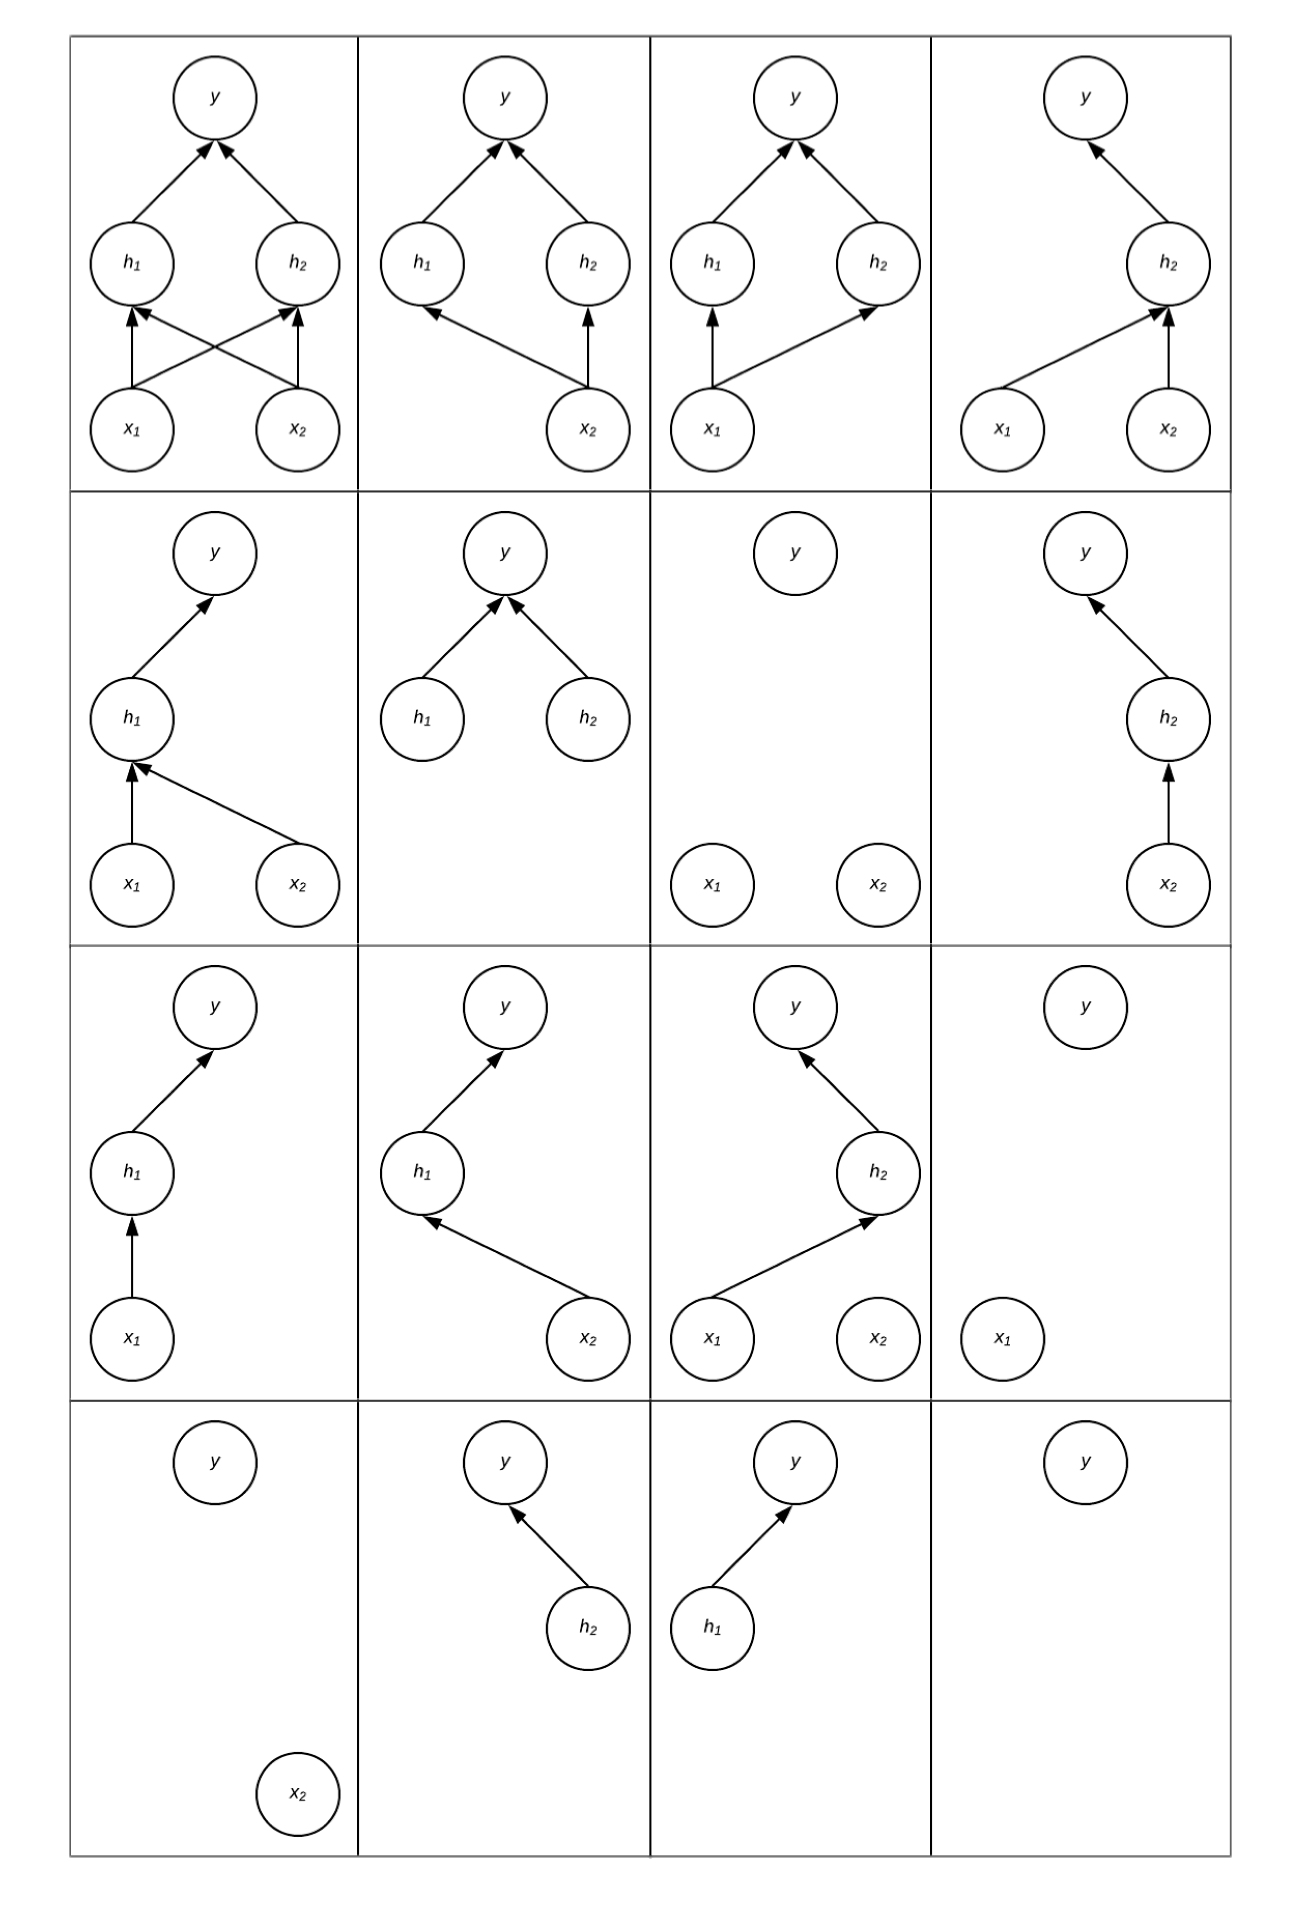
\includegraphics[scale=.25]{img/cap7_Dropout.png}
\end{figure}

\subsubsection{Otros m\'etodos de regularizaci\'on}
Otras formas de regularizaci\'on tambi\'en buscan introducir alguna fuente de ruido (como en dropout) para que la red neuronal aprenda principalmente los par\'ametros m\'as importantes, as\'i logrando un bajo error de generalizaci\'on. Una de estas t\'ecnicas es \textbf{dataset augmentation}, que consiste en generar nuevos datos de entrenamiento (inyectando ruido en el set de entrenamiento), creando datos $\bm{x}$ falsos para los cuales se pueda tener una etiqueta $y$ (por ejemplo, una imagen invertida de un gato sigue siendo un gato), o \textbf{entrenamiento adversarial}, en donde se perturban ejemplos para fortalecer a la red (por ejemplo, cambiar pixeles de una imagen que generen cambios imperceptibles para un humano pero que pueden afectar fuertemente la capacidad de predicci\'on de un modelo). Otra t\'ecnica es \textbf{noise injection} en los pesos (Jim et al., 1996; Graves, 2011), lo cual se puede interpretar como una implementaci\'on estoc\'astica de inferencia Bayesiana sobre los pesos, debido a que el aprendizaje considerar\'ia que los pesos son inciertos y, por lo tanto, representables mediante una distribuci\'on de probabilidad.

Tambi\'en, por supuesto, \textbf{early stopping} es una t\'ecnica v\'alida para regularizar redes neuronales.

\subsection{Algoritmos de optimizaci\'on}

Como ya se ha comentado, la optimizaci\'on en redes neuronales busca resolver un problema particular: encontrar los par\'ametros $\bm{\theta}$ que disminuyan significativamente $J(\bm{\theta})$, que depende de alguna medida de desempe{\~{n}}o evaluada en la totalidad del set de entrenamiento, luego se evaluá el error en el set de validaci\'on para tener una idea del desempeño, finalmente se ven los resultados en el set de testeo. 

Esto se reduce a minimizar la esperanza del error sobre la distribuci\'on generadora de los datos, $p_{\textrm{data}}$:

%[ posiblemente minimizando mediante hiperpar\'ametros tambi\'en una funci\'on de costos regularizada $\tilde{J}(\bm{\theta})$ ]

\begin{equation}
J^{*}(\bm{\theta}) = \E_{(\bm{x},y)\sim {p}_{\textrm{data}}}L(f(\bm{x};\bm{\theta}),y)
\label{gradiente_completo}
\end{equation}

Reemplazamos la expresión anterior por un problema sustituto, que consiste en escribir la funci\'on de costos como un promedio sobre el set de entrenamiento, como se puede observar la diferencia entre las dos expresiones radica en el hecho que se considera que los datos fueron generados por distribuciones de probabilidad distintas (${p}_{\textrm{data}}$ en la primera expresión, $\hat{p}_{\textrm{data}}$ en la segunda):

\begin{equation}
J(\bm{\theta}) = \E_{(\bm{x},y)\sim \hat{p}_{\textrm{data}}}L(f(\bm{x};\bm{\theta}),y) = \frac{1}{m}\sum_{i=1}^m L(f(x^{(i)};\theta),y^{(i)})
\end{equation}

\subsubsection{Minibatch}

Los algoritmos de optimizaci\'on para aprendizaje de m\'aquinas t\'ipicamente actualizan los par\'ametros usando un valor esperado del costo, obtenido a trav\'es de un subset de los t\'erminos de la funci\'on de costos. La propiedad m\'as usada respecto de la funci\'on objetivo (1) es sobre el gradiente, este cumple la siguiente expresión:

\begin{equation}
\nabla_{\bm{\theta}}J(\bm{\theta}) = -\E_{\bm{x},y\sim \hat{p}_{\textrm{data}}}\nabla_{\bm{\theta}}\textrm{log}\; p_{\textrm{modelo}}(y|\bm{x})
\end{equation}

Calcular esta expresi\'on es computacionalmente caro, ya que requiere evaluar cada ejemplo del set de entrenamiento, por lo que se puede optar por samplear un peque{\~{n}}o n\'umero de ejemplos para obtener este valor esperado, calculando el promedio usando solo estos ejemplos. Los algoritmos de optimizaci\'on que usan el set de entrenamiento completo para actualizar los par\'ametros en cada iteraci\'on se conocen como \textbf{m\'etodos de batch} o \textbf{determin\'isticos}. Los algoritmos que usan un solo ejemplo a la vez se conocen como \textbf{m\'etodos estoc\'asticos} u \textbf{online} (aunque el t\'ermino \textit{online} se suele usar para describir un entrenamiento con un flujo continuo de nuevos ejemplos). La mayor\'ia de los algoritmos usados pertenecen a una categor\'ia intermedia, estos son los \textbf{m\'etodos de minibatch} o \textbf{minibatch estoc\'astico}, los cuales usan un subconjunto de tamaño reducido de la totalidad de los ejemplos. Un criterio gu\'ia para decidir el n\'umero de batches a usar, es que batches m\'as grandes proveen estimadores m\'as precisos del gradiente, en este caso se obtienen retornos menores a uno lineal.

Una motivaci\'on importante para usar descenso de gradiente por mini-batches es que sigue el gradiente del costo que considera el error de generalizaci\'on (\ref{gradiente_completo}) mientras no se repitan ejemplos. En la pr\'actica las implementaciones de descenso del gradiente por mini-batches desordenan el set de datos una vez y luego pasan por \'el m\'ultiples veces.

\subsubsection{Algoritmos con momentum}

Aunque los métodos de descenso de gradiente estoc\'astico sigue siendo un algoritmo popular, el aprendizaje a veces puede ser lento. Los algoritmos que incorporan momentum fueron dise{\~{n}}ados para acelerar el aprendizaje, especialmente en presencia de altas curvaturas, cuando se tienen gradientes peque{\~{n}}os pero consistentes o gradientes ruidosos. El algoritmo \textbf{descenso de gradiente estoc\'astico con momentum} acumula un decaimiento exponencial de media m\'ovil de los gradientes pasados y contin\'ua su movimiento en esta direcci\'on. Un hiperpar\'ametro $\alpha$ determina qu\'e tan r\'apido las contribuciones de gradientes pasados decaen exponencialmente. Se actualiza mediante:

\begin{gather*}
\bm{v} \longleftarrow \alpha\bm{v} - \epsilon\nabla_{\bm{\theta}}\Big(\frac{1}{m}\sum_{i=1}^{m}L(f(\bm{x}^{(i)};\bm{\theta}),y^{(i)})\Big)
\\
\theta \longleftarrow \theta + \bm{v}
\end{gather*}

Con $\epsilon$ el learning rate y $\bm{v}$ la velocidad o momentum.

\subsubsection{Algoritmos con learning rates adaptativos}

En la pr\'actica el learning rate resulta ser uno de los hiperpar\'ametros m\'as dif\'iciles de ajustar debido a su importante efecto en el desempe{\~{n}}o del modelo. La funci\'on de costos suele ser altamente sensible (a crecer o decrecer) en algunas direcciones en el espacio de los par\'ametros e insensible en otras, por lo que hace sentido usar un learning rate distinto para cada par\'ametro y autom\'aticamente adaptar este par\'ametro durante el aprendizaje. El algoritmo \textbf{AdaGrad} adapta el learning rate de todos los par\'ametros al escalarlos de manera inversamente proporcional a la ra\'iz cuadrada de la suma de todos las ra\'ices cuadradas hist\'oricas del gradiente. Los par\'ametros con derivadas parciales m\'as grandes tienen un r\'apido decrecimiento en su learning rate, mientras que los par\'ametros con derivadas parciales peque{\~{n}}as decrecen en menor cantidad su learning rate. El efecto neto es mayor progreso en zonas m\'as planas del espacio de los par\'ametros. Se actualiza mediante:

\begin{gather*}
\delta = 10^{-7}; \bm{r} = 0\\
\bm{g} \longleftarrow \frac{1}{m}\nabla_{\bm{\theta}}\sum_{i=1}^{m}L(f(\bm{x}^{(i)};\bm{\theta}),y^{(i)})\\
\bm{r} \longleftarrow \bm{r} + \bm{g}\odot \bm{g}\\
\bigtriangleup\bm{\theta} \longleftarrow -\frac{\epsilon}{\delta+\sqrt{\bm{r}}}\odot \bm{g}\\
\bm{\theta} \longleftarrow \bm{\theta}+\bigtriangleup\bm{\theta}
\end{gather*}

Con $\delta$ una constante peque{\~{n}}a para estabilidad num\'erica (puede ser otra), $\bm{r}$ la variable de acumulaci\'on del gradiente, $\bm{g}$ el gradiente para el batch, y $\bigtriangleup\bm{\theta}$ la actualizaci\'on de los par\'ametros al final de una iteraci\'on.

Otras generalizaciones populares son el algoritmo \textbf{RMSProp}, que modifica el algoritmo AdaGrad para tener un mejor desempe{\~{n}}o en funciones no convexas al cambiar la acumulaci\'on del gradiente por una media m\'ovil que decae exponencialmente, y el algoritmo \textbf{Adam}, que combina RMSProp con momentum (con algunas distinciones importantes).

Hasta el momento no hay un algoritmo que tenga un desempe{\~{n}}o superior al de los dem\'as en distintos escenarios (Schaul et al., 2014), por lo que se recomienda usar el algoritmo de optimizaci\'on con el que el usuario se sienta m\'as c\'omodo al momento de ajustar los hiperpar\'ametros.

\subsection{Deep Learning y otros tipos de redes neuronales}

El t\'ermino \textbf{deep learning} se asocia a resolver problemas m\'as intuitivos (y f\'aciles) para los humanos que hasta hace solo algunos a{\~{n}}os eran extremadamente dif\'iciles para una m\'aquina, como lo son el reconocimiento de objetos en im\'agenes (visi\'on de computadores), la traducci\'on de texto desde un lenguaje a otro (machine translation), reconocimiento de voz, entre otros. Los problemas m\'as dif\'iciles para los humanos ya se han estado resolviendo hace mucho tiempo antes del deep learning, como divisar una estrategia ganadora en ajedrez (\url{https://en.wikipedia.org/wiki/Deep_Blue_versus_Garry_Kasparov}), aunque las redes neuronales profundas han seguido progresando en resolver este tipo de problemas (\url{https://deepmind.com/research/alphago/}). Las arquitecturas principales que han permitido resolver estos problemas en los \'ultimos a{\~{n}}os (sumado a los avances en poder de computaci\'on y cantidad de datos que existen hoy) se presentan en esta secci\'on: las \textbf{redes convolucionales} para procesamiento de im\'agenes, y las \textbf{redes recurrentes} para modelar series de tiempo (e.g., texto, audio). Tambi\'en se presentan otras arquitecturas que son tema activo de investigaci\'on en deep learning.: los \textbf{autoencoders} y las \textbf{redes generativas adversariales}.

\subsubsection{Redes neuronales convolucionales}

Las \textbf{redes neuronales convolucionales} (o \textbf{CNNs}) son un tipo de redes neuronales que fueron dise{\~{n}}adas para procesar datos con una tipolog\'ia tipo-\textit{grid} (grilla). Una serie de tiempo que tiene observaciones en intervalos regulares de tiempo se puede pensar como un \textit{grid} de 1 dimensi\'on. Las im\'agenes se pueden pensar como \textit{grids} de 2-D de pixeles. El nombre de esta arquitectura hace referencia a que usan una operaci\'on matem\'atica conocida como convoluci\'on.

La operaci\'on de \textbf{convoluci\'on} se define como:

\begin{equation}
s(t) = (x * w)(t) = \int x(a)w(t-a)da
\end{equation}

En el contexto de CNNs, el primer argumento a convolucionar, $x$, es el \textbf{input}, y el segundo argumento, $w$, se conoce como el \textbf{kernel}. El output, $s(t)$ se conoce como \textbf{feature map}. En aplicaciones de aprendizaje de m\'aquinas, el input ser\'an un arreglo multidimensional de datos, y el kernel un arreglo multidimensional de par\'ametros que se buscar\'an aprender. Usualmente, al trabajar con datos en un computador el tiempo se considerar\'a discreto, por lo que resulta conveniente definir la operaci\'on de convoluci\'on discreta:

\begin{equation}
s(t) = (x * w)(t) = \sum_{a=-\infty}^{\infty} x(a)w(t-a)
\end{equation}

Se asumir\'a que las funciones son 0 en todo su dominio excepto en el set finito de puntos para el cual se guardan valores, permitiendo realizar estas sumatorias infinitas. Las librer\'ias de redes neuronales implementan la funci\'on \textbf{cross-correlation} y la llaman convoluci\'on. Para una imagen $I$ de 2 dimensiones y un kernel K de 2 dimensiones, esto es: 

\begin{equation}
S(i,j) = (I * K)(i,j) = \sum_{m}\sum_{n} I(i+m,j+n)K(m,n)
\end{equation}

Esto es equivalente a la operaci\'on de convoluci\'on discreta con la diferencia que el operador no es conmutativo, $S(i,j) = (I * K)(i,j) \neq (K * I)(i,j)$, lo cual no es importante para implementaciones de redes neuronales. 

%[, con la diferencia de que no se puede cambiar el kernel relativo al input]

La motivaci\'on por usar convoluciones surge de 3 importantes propiedades: interacciones \textit{sparse}, \textit{parameter sharing}, y representaciones equivariantes. \textbf{Interacciones sparse} se refiere a que hay menos conexiones que en una red \textit{fully connected}, esto mediante el uso de kernels de menor dimensionalidad que el input, lo cual implica una eficiencia en t\'erminos de memoria por tener que almacenar menos par\'ametros, y eficiencia computacional por realizar menos operaciones. \textbf{Parameter sharing} se refiere a usar los mismo par\'ametros para distintas funciones dentro del modelo. Esto implica usar los pesos aprendidos en m\'ultiples partes del input (como para reconocer bordes, por ejemplo). Que una funci\'on sea \textbf{equivariante} significa que si el input cambia, el output cambia de la misma forma. Esto permite que en im\'agenes la convoluci\'on cree un map 2-D d\'onde ciertos atributos aparecen en el input.

Una capa t\'ipica de una red convolucional consta de 3 etapas: primero, aplicar varias convoluciones para producir un set de activaciones lineales. Luego, aplicar una activaci\'on no lineal (\textbf{detector stage}). Finalmente, una funci\'on de \textit{pooling} para modificar a\'un m\'as el output de la capa (ver figura). Una funci\'on de \textbf{pooling} reemplaza el output de la red en alguna locaci\'on por estad\'isticos de los outputs cercanos. 

\begin{figure}[H]
\captionsetup{font=small,labelfont=small}
\caption{Capa de una red convolucional}
\centering
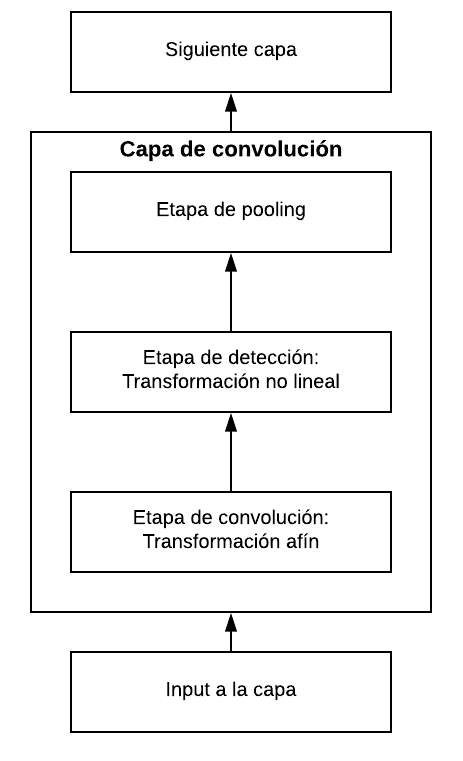
\includegraphics[scale=.8]{img/cap7_CNN.png}
\end{figure}

\textbf{Max pooling} retorna el valor m\'aximo de un output en una vecindad rectangular. Las operaciones de pooling permiten que la red sea invariante a peque{\~{n}}as transformaciones en el input. Pooling tambi\'en es escencial para procesar inputs de tama{\~{n}}o variable (por ejemplo im\'agenes de distinto tama{\~{n}}o).

Otras diferencias con respecto a la operaci\'on de convoluci\'on en el contexto de redes neuronales son, por ejemplo, el aplicar m\'ultiples convoluciones en paralelo, esto permite extraer distintos tipos de atributos en vez de 1 solo. Por otro lado, el \textbf{stride} hace referencia a cada cu\'antos pixeles se quieren convolucionar en cada direcci\'on en el output. En la figura se muestra el ejemplo de una convoluci\'on con stride. Esta operaci\'on permite reducir nuevamente el costo computacional. Esto tambi\'en implica que el output disminuye su tama{\~{n}}o en cada capa. El uso de \textit{padding} puede revertir esto. \textbf{Padding} se refiere a agrandar el input con ceros para hacerlo m\'as amplio. Una convoluci\'on en la que no se usa \textbf{zero-padding} se conoce como \textbf{valid}. Una convoluci\'on que mantiene el tama{\~{n}}o desde el input al output se conoce como \textbf{same} (ver figura). En la pr\'actica, las capas de una red convolucional usan operaciones entre una convoluci\'on valid y same.

\begin{figure}[H]
\captionsetup{font=small,labelfont=small}
\caption{Convoluci\'on con un stride igual a 2}
\centering
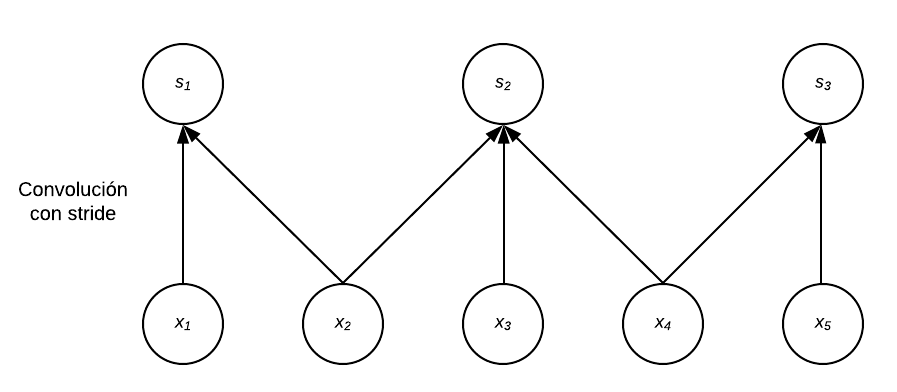
\includegraphics[scale=.8]{img/cap7_stride.png}
\end{figure}

\begin{figure}[H]
\captionsetup{font=small,labelfont=small}
\caption{Efecto de no usar zero-padding en una red convolucional (Arriba) y efecto de usar zero padding en una red convolucional (Abajo) en cuanto al tama{\~{n}}o de la red}
\centering
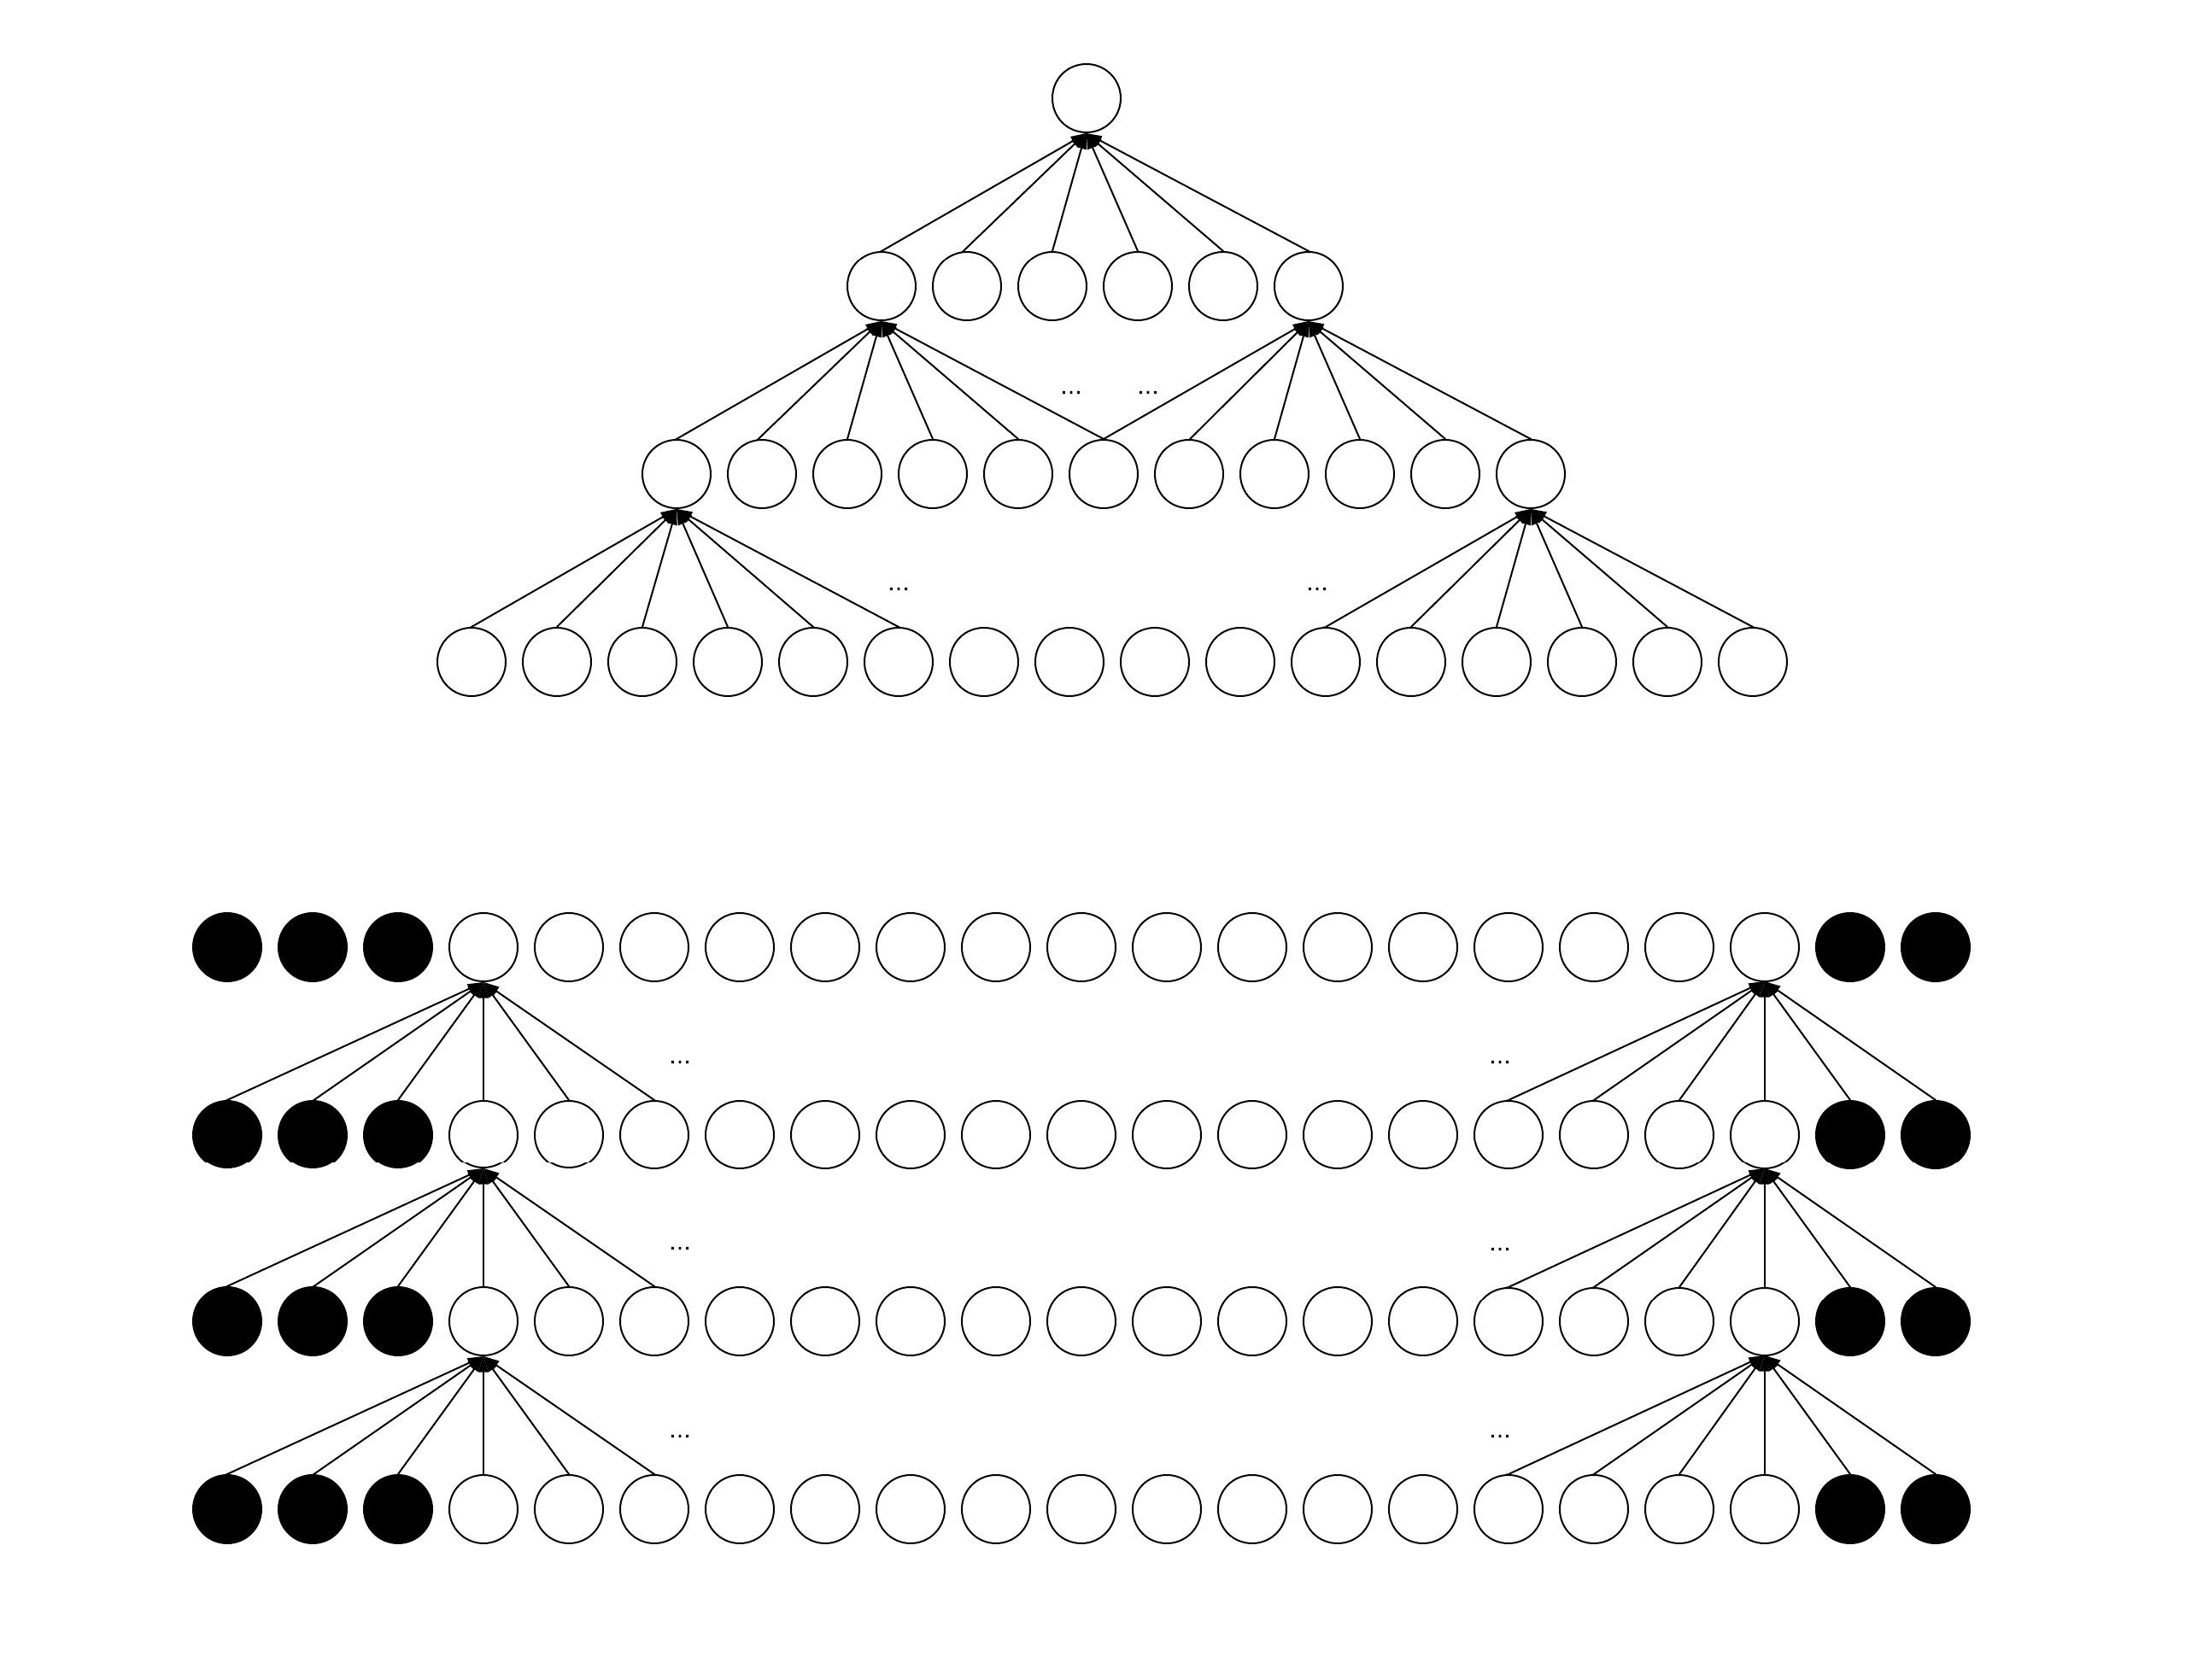
\includegraphics[scale=.15]{img/cap7_padding.png}
\end{figure}

\subsubsection{Redes neuronales recurrentes}

Las \textbf{redes neuronales recurrentes} o \textbf{RNNs} son una familia modelos de redes neuronales especializados para procesar datos secuenciales, $\bm{x}^{(1)},...,\bm{x}^{(\tau)}$. Las RNNs tambi\'en comparten par\'ametros, pero en una forma muy distinta que las CNNs. En una RNN, cada miembro del output en una etapa es una funci\'on de cada miembro del output de la etapa anterior.

Se denota por $\bm{h}^{(t)}$ al estado de un sistema din\'amico que involucra una recurrencia conducido por un input externo $\bm{x}^{(t)}$:

\begin{equation}
\bm{h}^{(t)} = f(\bm{h}^{(t-1)}; \bm{x}^{(t)}, \bm{\theta})
\end{equation}

La figura siguiente muestra una red recurrente que procesa un input $\bm{x}$ incorpor\'andolo al estado $\bm{h}$ que es traspasado a trav\'es del tiempo.

\begin{figure}[H]
\captionsetup{font=small,labelfont=small}
\caption{Ejemplo de una red recurrente sin output}
\centering
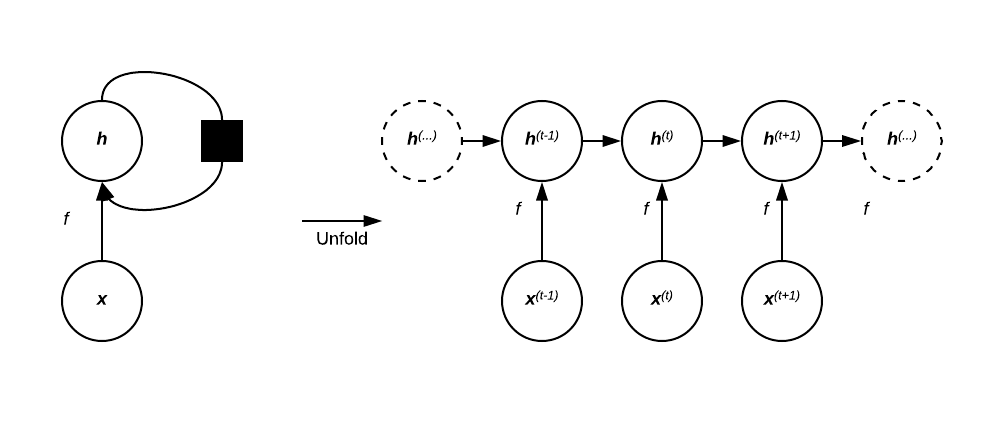
\includegraphics[scale=.5]{img/cap7_RNN1.png}
\end{figure}

Las redes recurrentes se pueden construir de muchas formas distintas. Al igual que una red neuronal puede representar casi cualquier funci\'on, una red recurrente modela cualquier funci\'on que involucre una recurrencia. Se puede representar el estado de una red recurrente luego de $t$ pasos mediante una funci\'on $g^{(t)}$:

\begin{equation}
\bm{h}^{(t)} = g^{(t)}(\bm{x}^{(t)},\bm{x}^{(t-1)},...,\bm{x}^{(1)}) =  f(\bm{h}^{(t-1)}; \bm{x}^{(t)}, \bm{\theta})
\end{equation}

Existen varios tipos de RNNs que se han dise{\~{n}}ado para distintos fines. Algunos ejemplos de estas son:

\begin{itemize}
  \item Redes recurrentes que producen un output en cada instante de tiempo y tienen conexiones entre todas las unidades escondidas
  \item Redes recurrentes que producen un output en cada instante de tiempo y tienen conexiones entre el output a la unidad escondida del siguiente instante
  \item Redes recurrentes con conexiones entre las unidad escondidas, que procesan una secuencia entera antes de producir el output
\end{itemize}

La figura muestra un ejemplo de la arquitectura para el primer caso.

\begin{figure}[H]
\captionsetup{font=small,labelfont=small}
\caption{Ejemplo de una red recurrente que produce un output en cada instante de tiempo, y que comparte el estado a trav\'es del tiempo}
\centering
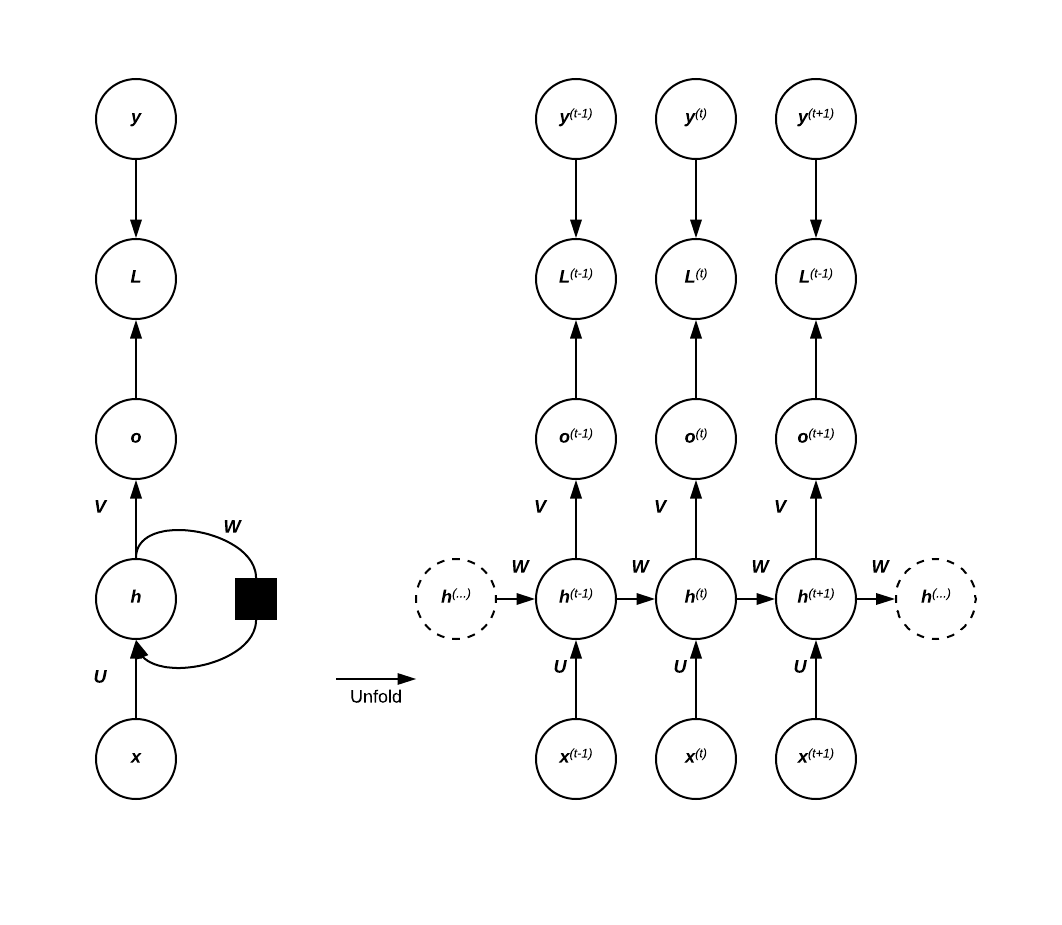
\includegraphics[scale=.5]{img/cap7_RNN2.png}
\end{figure}

Esta red presentada puede ser usada para producir palabras en cada instante, y as\'i producir oraciones que hagan sentido en una conversaci\'on. Como ejemplo de entrenamiento de una red con esta arquitectura, en donde en la \'ultima capa se decide mediante una funci\'on softmax la palabra m\'as probable que deba seguir a la palabra anterior, se tienen las ecuaciones de \textit{forward propagation} para cada instante de tiempo:

\begin{equation}
\begin{array}{l}
\bm{a}^{(t)} = \bm{b} + \bm{W}\bm{h}^{(t-1)}+\bm{U}\bm{x}^{(t-1)} \\
\bm{h}^{(t)} = \textrm{tanh}(\bm{a}^{(t)}) \\
\bm{o}^{(t)} = \bm{c} + \bm{V}\bm{h}^{(t)} \\
\hat{\bm{y}}^{(t)} = \textrm{softmax}(\bm{o}^{(t)})
\end{array}
\end{equation}

El algoritmo aplicado para obtener el gradiente en este tipo de arquitectura se conoce como \textbf{back-propagation through time}, y consiste en aplicar el algoritmo de \textit{back-propagation} generalizado para el grafo computacional \textit{unfolded} de la red, como los mostrados en las figuras de redes recurrentes.

Las redes recurrentes sufren de no poder recordar largas dependencias a trav\'es del tiempo, debido a que las recurrencias implican multiplicar una matriz de pesos m\'ultiples veces a trav\'es de la red, provocando superficies planas o muy empinadas que resultan en que los algoritmos de aprendizaje por gradiente tengan problemas de \textbf{vanishing gradients} o \textbf{exploding gradients}, respectivamente. Arquitecturas que han logrado superar esto son las que incluyen compuertas (funciones sigmoidales) que deciden autom\'aticamente qu\'e olvidar y qu\'e seguir propagando a trav\'es de la red. Estos son los modelos de \textbf{gated recurrent units} (\textbf{GRUs}) y \textbf{long-short term memory network} (\textbf{LSTM}).

\subsubsection{Autoencoders}

Un \textbf{autoencoder} es una red neuronal que busca replicar el input hacia el output, osea, se busca que la información que entra a la red sea lo más parecida posible a la de salida, para lo cual cuenta con una capa interna $\bm{h} = f(\bm{x})$ que codifica el input (genera una representaci\'on de este) llamada \textbf{encoder} y una funci\'on que produce la reconstrucci\'on $\bm{r} = g(\bm{h})$, el \textbf{decoder}. Un \textit{autoencoder} buscar\'a aprender los \textit{encoder} y \textit{decoder} tales que $g(f(\bm{x})) = \bm{x}$ para todo $\bm{x}$. Como el modelo est\'a forzado a aprender los atributos m\'as importantes para que pueda efectivamente reproducir el input en su output, este aprender\'a en general propiedades \'utiles de los datos de entrenamiento. Los \textit{autoencoders} modernos modelan mappings estoc\'asticos $p_{\textrm{encoder}}(\bm{h}|\bm{x})$ y $p_{\textrm{decoder}}(\bm{x}|\bm{h})$, en vez de funciones determin\'isticas. En la figura se muestra la arquitectura de un \textit{autoencoder}.

\begin{figure}[H]
\captionsetup{font=small,labelfont=small}
\caption{Estructura de un \textit{autoencoder} t\'ipico}
\centering
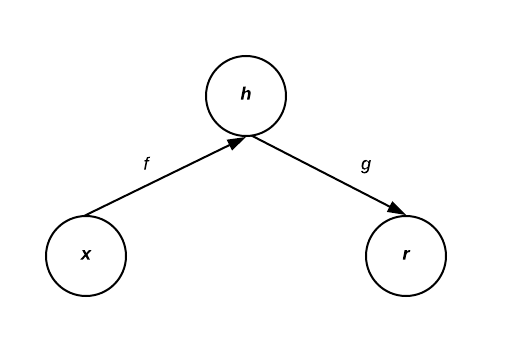
\includegraphics[scale=.8]{img/cap7_autoencoder.png}
\end{figure}

Una manera de obtener atributos \'utiles de $\bm{x}$ es forzando a que el \textit{encoder} tenga una dimensionalidad menor que el input. Este tipo de \textit{autoencoders} se denominan \textbf{undercomplete}. El aprendizaje se describe mediante la optimizaci\'on de la funci\'on de p\'erdida, $L(\bm{x}, g(f(\bm{x})))$. Cuando el \textit{decoder} es lineal y la funci\'on de p\'erdida es el error cuadr\'atico medio, un \textit{undercomplete autoencoder} aprende a generar el mismo subespacio que el algoritmo \textbf{principal component analysis} (\textbf{PCA}), es decir, el \textit{autoencoder} que fue entrenado para reproducir los datos de entrenamiento mediante una reducci\'on de dimensionalidad y una reconstrucci\'on aprendi\'o como efecto colateral el subespacio principal. Es as\'i como entonces, \textit{autoencoders} con \textit{encoders} y \textit{decoders} no lineales pueden aprender representaciones no lineales m\'as poderosas que PCA.

Un \textit{autoencoder} con dimensi\'on de su \textit{encoder} igual a la del input se conoce como \textbf{overcomplete}. Estos \textit{autoencoders}, al igual que los \textit{undercomplete}, pueden fallar en aprender una representaci\'on \'util del input si tienen mucha capacidad, por lo que ser\'a importante tambi\'en regularizar estas redes neuronales.

Otras aplicaciones de los autoencoders, aparte de aprender una reducci\'on de dimensionalidad, es aprender representaciones \'utiles que sirvan para un posterior modelo de redes neuronales (o, m\'as general, de aprendizaje de m\'aquinas). Por ejemplo, en vez de usar \textbf{one-hot-vectors} para representar palabras (en donde se tiene un vector del largo de cierto vocabulario compuesto por ceros excepto para la palabra que se quiere representar, indicando un valor de 1 en esa posici\'on), se pueden usar \textbf{embeddings}, que son representaciones del input a un espacio de valores reales. A diferencia de los \textit{one-hot-vectors}, en un \textit{embedding} la distancia entre las representaciones del texto s\'i tiene un significado, y este tipo de representaciones podr\'ia entregar mejores resultados en la tarea en que se est\'e usando.

\subsubsection{Redes generativas adversariales}

Una \textbf{red generativa adversarial} (o \textbf{GAN}) se basa en un escenario de teor\'ia de juegos, en donde una \textbf{red generadora} debe competir con un adversario. La red generadora produce muestras $\bm{x} = g(\bm{z};\bm{\theta}^{(g)})$, mientras que una \textbf{red discriminadora} trata de distinguir entre muestras obtenidas de los datos de entrenamiento y muestras generadas por la red generadora. El discriminador retorna una probabilidad, $d(\bm{x};\bm{\theta}^{(d)})$, indicando la probabilidad de que $\bm{x}$ sea un dato real y no uno simulado.

Para formular el aprendizaje, se describe un juego de suma cero en donde una funci\'on $v(\bm{\theta}^{(g)},\bm{\theta}^{(d)})$ determina el pago del discriminador, y el generador recibe $-v(\bm{\theta}^{(g)},\bm{\theta}^{(d)})$ como pago. As\'i, durante el entrenamiento cada jugador intenta maximizar su propio pago, para que en convergencia se tenga

\begin{equation}
g^{*} = \textrm{arg} \textrm{min}_{g} \textrm{max}_{d} v(g,d)
\end{equation}

Esto motiva a que el discriminador aprenda a clasificar correctamente entre muestras reales y falsas y, simulat\'aneamente, el generador intenta enga{\~{n}}ar al clasificador para que crea que las muestras generadas son reales. En convergencia, las muestras del generador son indistinguibles de los datos reales. Una motivaci\'on del uso de GANs es que cuando $\textrm{max}_{d} v(g,d)$ es convexa en $\bm{\theta}^{(g)}$, el procedimiento asegura la convergencia.

\begin{figure}[H]
\captionsetup{font=small,labelfont=small}
\caption{Im\'agenes generadas por una GAN entrenada con el set de datos LSUN. (Izquierda) Im\'agenes de dormitorios generadas por el modelo DCGAN (imagen de Radford et al., 2015). (Derecha) Im\'agenes de iglesias generadas por el modelo LAPGAN (imagen de Denton et al., 2015)}
\centering
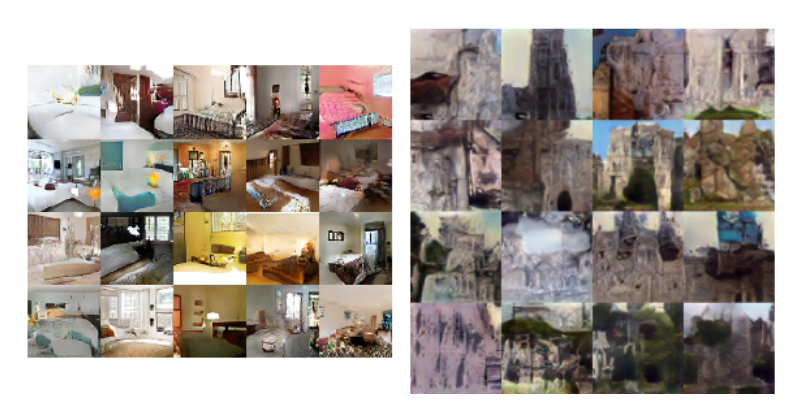
\includegraphics[scale=.75]{img/cap7_gans.PNG}
\end{figure}

%!TEX root = ../notas_de_clase.tex
\section{Support-vector machines}

Una de las desventajas de los clasificadores lineales vistos en el Capítulo \ref{cap:clasificacion} (en el caso binario) es la falta de atención al margen de las clases, es decir, la región entre las muestras de ambas clases, pues en esta región se encontrará el hiperplano de decisión. Esta distancia es relevante, pues nos da un sentido de generalización, es decir,  los elementos de la clase 1  \emph{más parecidos} a los de la clase -1 no están justo en el borde de las clases, sino que existe una zona donde podrían haber nuevas muestras en torno a datos existentes de clase, e.g., 1 y aún estar dentro de la región de clase 1. El tratamiento de este concepto (o la falta de él) es claro en los métodos anteriores: en el perceptrón, todas las soluciones que dividen las muestras clases $\pm 1$ son ``igual de buenas'', es decir, el perceptrón es insensible al margen descrito arriba. Por otro lado, para los métodos que funcionan mediante gradiente descendente como mínimos cuadrados o regresión logística, este margen se maximiza \emph{indirectamente}, lo cual conlleva a inestabilidades como en el caso en donde el parámetro de la regresión logística diverge. \\


Para resolver el problema descrito anteriormente consideraremos las \textbf{máquinas de soporte vectorial} (SVM, por sus siglas en inglés). Como veremos en este capítulo, además de resolver el problema de clasificación binaria y lineal, la solución de SVM puede ser ocupado en muchas más situaciones, por esta razón, dedicamos un capítulo completo a este método en vez de verlo como un método de clasificación más. 

\subsection{Idea general}

Consideremos un problema de clasificación donde las clases son linealmente separables. Como podemos ver en la Fig.~\ref{fig:maxim_marg} (izquierda), en este caso existen diferentes hiperplanos (clasificadores lineales) que separan los datos de ambas clases de forma correcta. Cada una de estas soluciones define un modelo, donde dado un nuevo dato $x_\star$, podemos evaluar a qué clase pertenece. Evidentemente, la asignación de clase usando cada uno de los clasificadores mostrados en la figura  anterior (izquierda) son similares en la mayoría del espacio salvo la región cercana al límite de las clases; es precisamente en este lugar donde nos enfocamos en este capítulo. 


\begin{figure}[ht]
    \centering
    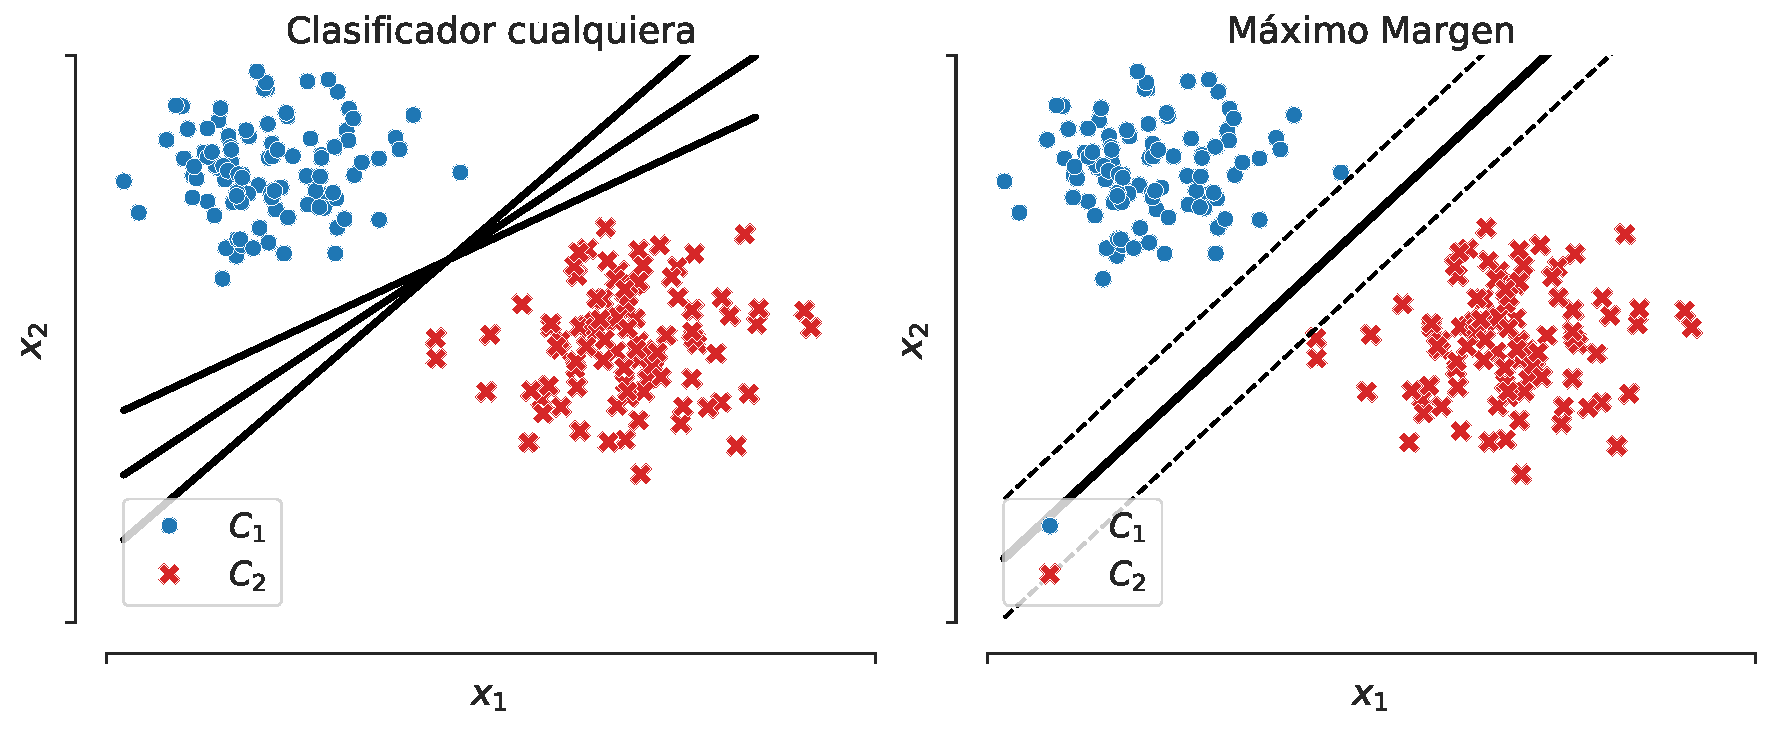
\includegraphics[width=0.9\textwidth]{img/cap5_max_margen.pdf}
    \caption{Clasificadores lineales: varios clasificadores (izquierda) y clasificador de máximo margen (derecha)}
    \label{fig:maxim_marg} 
\end{figure}

Aquí entonces aflora la siguiente pregunta, como todas los clasificadores en la Fig.~\ref{fig:maxim_marg} (izquierda) separan de forma correcta los datos disponibles, ¿cuál de ellos debemos elegir? Elegiremos un \emph{clasificador de máximo margen}, es decir, el clasificador que nos entregue la máxima separación entre los datos y las regiones definidas como correspondiente a cada clase. Una ilustración del clasificador de máximo margen se presenta en la Fig.~\ref{fig:maxim_marg} (derecha). En donde se ve que encontrar este clasificador es equivalente a encontrar una \emph{cinta} de ancho máximo que separe los datos de ambas clases.\\


El argumento de ocupar dicho criterio es la búsqueda de buenas propiedades de generalización. Intuitivamente, esta propiedad se obtiene debido a que asumiendo que los datos generados en cada clase  provienen de una distribución latente, es de esperar que si se obtienen nuevos datos desde la misma distribución, éstos estén cerca de los datos observados inicialmente. De este forma, con el máximo margen se pretende maximizar la probabilidad de que los nuevos datos de clase 1 (cf. -1) sean bien clasificados también.\\

Una propiedad clave del clasificador de máximo margen es que éste queda definido únicamente por algunos datos, ver Fig.~\ref{fig:maxim_marg} (derecha). Esto inmediatamente resuelve el problema de desbalances de clase o de que las clases tengan formas distintas (problema mencionado en clasificación con mínimos cuadrado o con el discriminante de Fisher). Es decir, la solución de máximo margen se mantiene si agregamos datos (de cualquier clase) que están fuera del margen. Los datos (o vectores, pues recordemos que $x\in\R^M$) que definen el margen los llamaremos vectores de soporte (\emph{support vectors}), cuya función es restringir la rotación y expansión del margen.\\

Finalmente, una diferencia fundamental entre un clasificador que se enfoca en el margen y otros métodos que que hemos visto (e.g., na\"ive Bayes, regresión lineal, regresión logística) es que éstos últimos aprenden incorporando todos los datos para formar la respuesta, no solo los que están en el margen. En cambio, SVM define el clasificador utilizando únicamente los vectores soporte ya que si bien todos los datos se debe analizar para encontrar los vectores soporte, los datos que no son vectores soporte no toman parte en la solución final (ni en las predicciones).

\subsection{Formulación del problema}

Denotemos un conjunto de entrenamiento $\{x_i\}_{i=1}^N$, con clases $\{1,-1\}$ linealmente separable y recordemos que un hiperplano de separación está definido mediante
\begin{equation}
    \{x\in \R^n | w^\top x + b = 0 \},\label{ec:hiperplano_svm}
\end{equation}
donde $w\in \R^n$ es el vector perpendicular al hiperplano y $b\in \R$ es el \emph{offset}. De esta forma, si $w^\top x + b >0$ se le asignará a $x$ la clase 1, mientras que si $w^\top x + b <0$ se le asignará a $x$ la clase -1.\\

El problema de clasificación consiste en encontrar dichos parámetros de acuerdo a algún criterio, en este caso es el criterio del máximo margen. Notemos en primer lugar que este problema no tiene solución única, pues si $(w,b)$ son solución entonces $(\lambda w, \lambda b)$, $\lambda>0$ también lo son. Para evitar esta \emph{invarianza} con tal de que el problema tenga solución única, podemos imponer una restricción sobre los bordes del margen. Denotando vectores soporte de cada clase mediante $x_{+}$ y $x_{-}$, se impone que para todo vector soporte $x_+$, $x_-$, estos pertenezcan a su respectiva clase, es decir:
\begin{align}
 	w^\top x_{+} + b &= 1 \label{ec:borde_svm1}\\
 	w^\top x_{-} + b &=  -1,\label{ec:borde_svm2}
 \end{align}
 donde estos vectores soportes puede no ser únicos. Observemos que si bien aún no sabemos cuales son los vectores de soporte, podemos imponer esta restricción de todas formas, las que se van a traducir en las restricciones del problema de optimización que definirá la solución del problema de clasificación.\\
 
 Además, es importante ver que las restricciones anteriores implican que $w\neq 0$, lo cual será importante más adelante cuando haya que justificar que el funcional a maximizar es estrictamente cóncavo.

Notemos que las ecs.~\eqref{ec:hiperplano_svm},\eqref{ec:borde_svm1} y \eqref{ec:borde_svm2} definen tres hiperplanos paralelos, pues todos tienen el mismo parámetro $w$. La Fig.~\ref{fig:clasif_margen} ilustra las muestras de cada clase junto con estos tres hiperplanos, donde además se muestra el vector unitario perpendicular a (todos) estos hiperplanos dado por $\frac{w}{||w||}$. El ancho del {margen}, denotado por $m$, es la distancia entre la región de decisión y cualquiera de las clases, y es igual a la mitad de la diferencia entre ambos vectores de soporte, proyectada en la dirección normal del hiperplano, es decir, 
\begin{align}
m &= \frac{1}{2} \norm{\operatorfont{proy}_w(x_+-x_-)} = \frac{1}{2} \norm{x_+-x_-}\cos(\theta) \\
&= \frac{1}{2}\norm{x_+-x_-} \left(\frac{w^\top(x_+-x_-)}{\norm{w}\cdot\norm{x_+-x_-}}\right)\\
& =\frac{1}{2\norm{w}} w^\top(x_+ - x_-)
\end{align}

Donde se usó el hecho de que $cos\left(\measuredangle(x,y)\right) = \frac{\langle x,y\rangle}{\norm{x}\norm{y}}$.

\begin{figure}[ht]
    \centering
    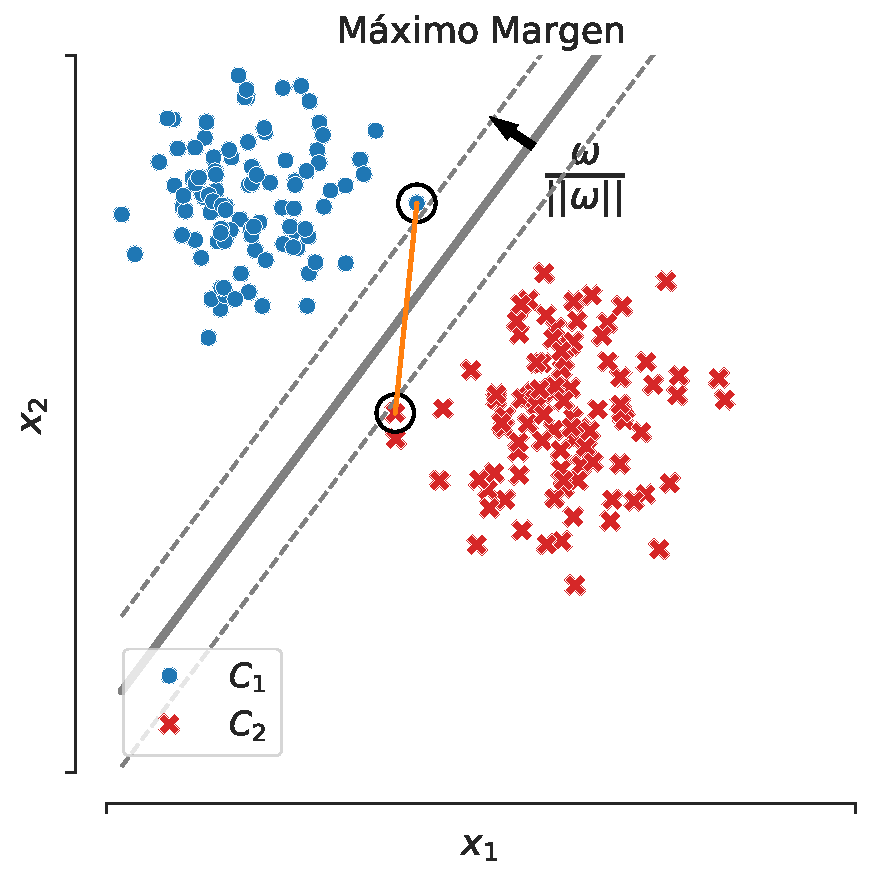
\includegraphics[width=0.4\textwidth]{img/cap5_max_margen2.pdf}
    \caption{Clasificación de máximo margen. Clases denotadas por puntos azules y cruces rojas, región de decisión en gris sólido y bordes del margen en línea punteada. La línea naranja representa la  el vector diferencia $(x_+ - x_{-})$ y la flecha negra el vector unitario $\frac{w}{||w||}$. Los vectores soporte están indicados con un círculo negro.}
    \label{fig:clasif_margen}
\end{figure}

Veamos que el ancho del margen $m$ no depende explícitamente de los vectores soporte al incorporar las restricciones en las ecs.~\eqref{ec:borde_svm1}-\eqref{ec:borde_svm2}:

\begin{align}
    m &= \frac{1}{2||w||} \left( (w^\top x_{+}) - (w^\top x_{-})\right)\nonumber\\
    &= \frac{1}{2||w||} \left((1-b) - (-1-b)\right)\nonumber\\
    &= \frac{1}{||w||}.\label{eq:margen}
\end{align}
Además, consideremos la siguiente codificación para las clases:
\begin{alignat}{3}
    y_i&=+1 &&\Leftrightarrow w^\top x_i + b \geq +1 \label{eq:codif_svm1}\\
    y_i &=-1 &&\Leftrightarrow w^\top x_i + b \leq -1.\label{eq:codif_svm2}
 \end{alignat}
 
En base a la expresión de la ec.~\eqref{eq:margen} para el ancho del margen y la codificación de clases anterior, podemos formular el problema de clasificación de máximo margen mediante  siguiente problema de optimización:
\begin{equation}
\begin{aligned}
& \underset{w,b}{\text{max}}
& & \frac{1}{||w||}\\
& \text{s.a}
& & y_i (w^\top x_i +b) \geq 1, \; i = 1, \ldots, N.
\end{aligned}
\end{equation}
Lo cual simplemente quiere decir que se está maximizando el ancho del margen, sujeto a que todas las muestras estén bien clasificadas. Es importante notar que este problema es factible solo si las clases son linealmente separable ya que restricción exige que todas las muestran queden bien clasificadas.\\

Para evitar problemas de diferenciablidad del recíproco de la raíz cuadrada en el objetivo del problema de optimización anterior, sobretodo cuando $w$ es cercano a 0, consideraremos la siguiente formulación equivalente del problema anterior:
\begin{equation}
\begin{aligned}
(P)\quad & \underset{w,b}{\min}
& & \frac{1}{2}||w||^2\\
& \text{s.a}
& & y_i (w^\top x_i +b) \geq 1, \; i = 1, \ldots, N.
\end{aligned}
\end{equation}
Este problema de optimización con restricciones puede ser resuelto mediante el método de Lagrange, donde resolvemos el \emph{problema dual} (ver anexos), el cual tiene una estructura más ``amigable'' para resolver. Además, luego veremos que la resolución mediante este método es fundamental para la extensión no-lineal de SVM.\\

El lagrangiano del problema anterior está dado por:
\begin{equation}
    L(w,b,\alpha) = \frac{1}{2}||w||^2 + \sum\limits_{i=1}^{N} \alpha_i \left(1-y_i (w^\top x_i +b)\right)\label{eq:lagrangiaano_svm}
\end{equation}
donde hemos denotado los multiplicadores de Lagrange mediante $\alpha = (\alpha_1,\ldots,\alpha_N)^\top$. El lagrangiano dual del problema viene dado por $\theta(\alpha) = \inf\limits_{w,b} L(w,b,\alpha)$ y dado que $L$ es convexo, basta aplicar la condición de primer orden:
\begin{align}
	&\frac{\partial L}{\partial w} = w^\top - \sum_{i=1}^N \alpha_i y_i x_i^\top = 0 \implies \overline{w} = \sum_{i=1}^N \alpha_i y_i x_i\\
	&\frac{\partial L}{\partial b} = -\sum_{i=1}^N \alpha_i y_i = 0 \implies \sum_{i=1}^N \alpha_i y_i = 0
\end{align}

Por lo tanto, el lagrangiano dual tiene la siguiente forma:
\begin{align}
	\theta(\alpha) &= L(\overline{w},\overline{b},\alpha) = \frac{1}{2} \left\langle \sum_{i=1}^N \alpha_i y_i x_i,\sum_{j=1}^N \alpha_j y_j x_j \right\rangle + \sum_{i=1}^N \alpha_i - \sum_{i=1}^N \alpha_i y_i \left\langle\sum_{j=1}^N \alpha_j y_j x_j , x_i \right\rangle - b\sum_{i=1}^N \alpha_i y_i  \\
	&= \frac{1}{2} \sum_{i,j=1}^N \alpha_i y_i \alpha_j y_j \langle x_i,x_j\rangle + \sum_{i=1}^N \alpha_i - \sum_{i,j=1}^N \alpha_i y_i \alpha_j y_j \langle x_j,x_i\rangle = \sum_{i=1}^N \alpha_i - \frac{1}{2} \sum_{i,j=1}^N \alpha_i \alpha_j y_i y_j \langle x_i,x_j\rangle
\end{align}

Donde en la penúltima igualdad se usó el hecho de que $\sum\limits_{i=1}^N \alpha_i y_i = 0$ de acuerdo a la segunda CPO sobre $L$.\\

Finalmente, el problema dual consiste en maximizar $\theta(\alpha)$ sujeto a que $\alpha\geq 0$, es decir:


\begin{equation}
\begin{aligned}
(D)\quad & \underset{\alpha}{\max}
& & \sum\limits_{i=1}^{N}\alpha_i - \frac{1}{2} \sum\limits_{i,j=1}^{N} \alpha_i \alpha_j y_i y_j \langle x_i, x_j\rangle\\
& \text{s.a}
& & \sum\limits_{i=1}^{N} \alpha_i y_i= 0 \\
& &  &\alpha_i \geq 0
\end{aligned} \label{eq:dualSVM}
\end{equation}

La segunda restricción se heredó de la CPO impuesta sobre $L$ al calcular $\theta(\alpha)$. Este problema es del tipo QP (\emph{quadratic programming}), para el cual existen variados métodos para resolverlo de manera óptima y eficiente. Por otra parte,

\begin{equation}
\sum\limits_{i,j=1}^{N} \alpha_i \alpha_j y_i y_j \langle x_i, x_j\rangle = \sum\limits_{i,j=1}^{N}  \alpha_i \langle   y_i x_i,  y_jx_j\rangle \alpha_j = \alpha^\top \Lambda \alpha,
\end{equation}
 
Donde $\Lambda\in\R^{N\times N}$ corresponde a una matriz de Gram (en alguna base) por lo que es definida positiva ya que para $\alpha\neq 0$:

\begin{equation}
	\alpha^\top \Lambda \alpha = \sum\limits_{i,j=1}^{N}   \langle   \alpha_i y_i x_i,  \alpha_j y_jx_j\rangle = \left\langle\sum\limits_{i=1}^{N}      \alpha_i y_i x_i,  \sum\limits_{j=1} \alpha_j y_jx_j\right\rangle = \norm{\sum\limits_{i=1} \alpha_i y_i x_i}^2 = \norm{\overline{w}}^2>0 
\end{equation}

Además, se tiene la siguiente propiedad:

\begin{lemma}
	$A$ es definida positiva si y solo si $f(x)= x^tAx + b^tx + c$ es estrictamente convexa.
\end{lemma}

\begin{proof}
	Basta verlo para la forma cuadrática $f(x)=x^tAx$. Sea $\lambda\in (0,1)$ y $x,y\in\R^n$, entonces:

\begin{align*}
	&\left(\lambda x+(1-\lambda)y\right)^t A \left(\lambda x+(1-\lambda)y\right) \leq \lambda x^tAx + (1-\lambda)y^tAy\\
			\iff &\lambda^2 x^tAx + (1-\lambda)^2 y^tAy + \lambda(1-\lambda)x^tAy + \lambda(1-\lambda)y^tAx \leq \lambda x^t Ax+(1-\lambda)y^tAy\\
			\iff & \lambda(1-\lambda)x^tAx+\lambda(1-\lambda)y^tAy-\lambda(1-\lambda)y^tAy\geq 0\\
			\iff & x^tAx+y^tAy-x^tAy-y^tAx\geq 0\\
			\iff & (x-y)^tA(x-y)\geq 0, \forall x,y\in \R^n\\
			\iff &A \text{ es definida positiva}
\end{align*}
\end{proof}

Luego, el funcional de SVM es estríctamente cóncavo, lo cual implica que el máximo del problema es único.\\

 Una vez resuelta la formulación dual (i.e., se han encontrado los valores óptimos para $\alpha$), la predicción de un nuevo punto $x_\star$ es de la forma 
\begin{equation}
 	\hat{y}(x_\star)= \text{sgn} (\overline{w}^\top x_\star + b) = \text{sgn}\left(\left[\sum\limits_{i=1}^{N} \alpha_i y_i \langle x_i, x_\star\rangle\right] + b\right),
 \end{equation}
 
Finalmente, por el teorema de holgura complementaria, para $\alpha$ óptimo se tiene que
\begin{equation}
	\alpha_i \left(1-y_i (\overline{w}^\top x_i +b)\right) = 0,\quad \forall i\in\{1,\ldots,N\}\implies \alpha_i=0\text{ para todo $x_i$ fuera del margen.}
\end{equation}

y consecuentemente, $x_i$ no aporta en la predicción $\hat{y}$. Esta propiedad es la que mencionábamos al principio: la predicción de clase solo depende de los vectores soporte, i.e., los que están en el margen. Esto ayuda a resolver el problema de optimización de manera más rápida, ya que en realidad solo algunas variables duales $\alpha_i$ serán no nulas (las correspondiente a los vectores que están en el borde del margen). Normalmente se ocupan heurísticas para encontrar y descartar rápidamente que vectores no son de soporte y así resolver un problema mas simple (ver, por ejemplo, el método de \emph{Sequential Minimal Optimization}). 


\begin{remark} Notemos que las características $\{x_i\}$ solo aparecen en forma de productos internos entre ellas mismas en la solución del método SVM, lo cual se puede ver desde la formulación de problema de optimización dual en la ec.~\eqref{eq:dualSVM}. Esto es clave para la extensión no lineal de SVM, pues no necesitamos operar directamente  con los valores de las entradas o características, sino con los productos punto entre ellas. En particular, si tenemos $N$ entradas de $M$ dimensiones, solo necesitamos los $N(N+1)/2$ productos puntos entre ellos y no todos los $NM$ valores, lo cual es particularmente relevante en caso que $M$ sea muy grande o incluso cuando $M=\infty$ (e.g., cuando las características $\phi:x_i\mapsto \phi(x)$ son funciones).
\end{remark} 

\subsection{Margen suave}

El planteamiento anterior tiene dos debilidades: la primera es que nuestros datos no siempre serán separables, y la segunda es que, incluso si los datos son linealmente separables, nuestro clasificador puede ser muy sensible a nuevos datos. Esto es ilustrado en la Fig.~\ref{fig:svm_softmargin}, donde el clasificador de máximo margen sin \emph{outlier} (izquierda) es muy distinto, o no-robusto, al obtenido en el caso de un \emph{outlier} (encerrado en púrpura). En general, queremos que nuestro estimador sea robusto a este tipo de datos, tal como lo es la regresión lineal frente a observaciones ruidosas. 

\begin{figure}[ht]
    \centering
    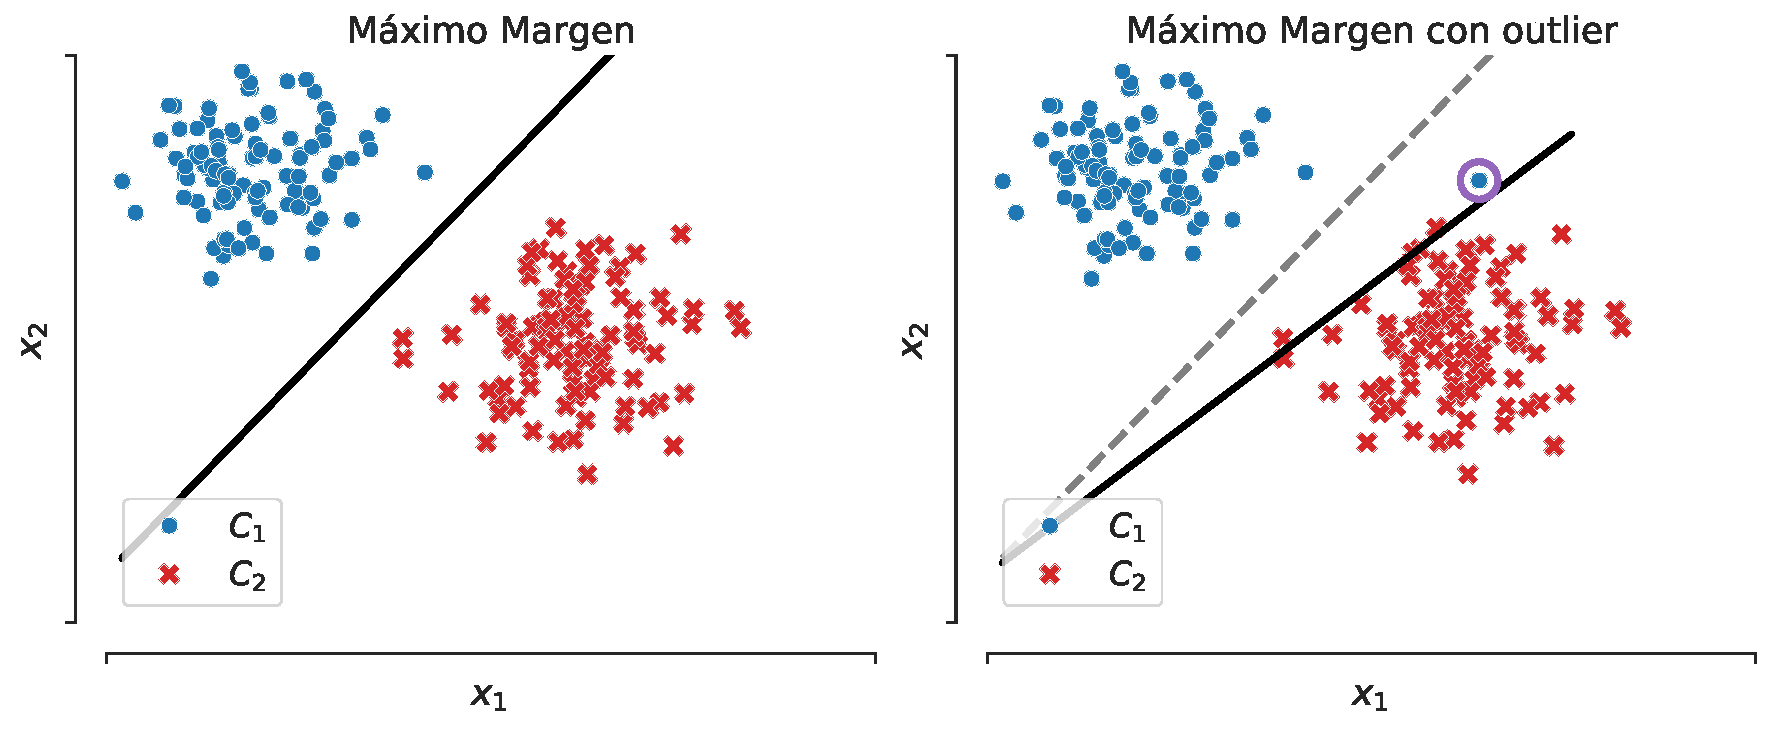
\includegraphics[width=0.9\textwidth]{img/cap5_margen_suave}
    \caption{Sensibilidad del máximo margen al agregar un nuevo dato: a la izquierda el caso sin \emph{outlier} y a la derecha el caso con \emph{outlier}, donde la solución anterior se muestra con la línea punteada.}
    \label{fig:svm_softmargin}
\end{figure}

Para considerar datos que son no posibles de clasificar con el clasificador lineal de máximo margen, podemos introducir las llamadas ``variables de holgura'' (\emph{slack variables}). Éstas tienen el objetivo de permitir al clasificador admitir algunos datos incorrectamente clasificados, aún maximizando el margen. Específicamente, esto se logra reemplazando las restricciones para los datos mal clasificados (considerados \emph{outliers}) directamente en la formulación del problema de optimización, de esta forma, la \textit{mayoría} de los datos se clasifican de forma correcta con la finalidad de tener un modelo robusto.

La formulación del problema de clasificación que \emph{perdona} algunos datos mal clasificados mediante la utilización de variables de holgura $\{\xi_i\}_{i=1}^N$ es la siguiente:

\begin{equation}
\begin{aligned}
(P)\quad & \underset{w,b, \xi}{\text{min}}
& & \frac{1}{2}||w||^2 + c\sum\limits_{i=1}^{N} \xi_i \\
& \text{s.a}
& & y_i (w\cdot x_i +b) \geq 1 - \xi_i,\;\xi_i\geq0,\; i = 1, \ldots, N
\end{aligned}
\end{equation}
donde $c>0$ es un hiperparámetro. Observemos que la introducción del término $c\sum_{i=1}^{N} \xi_i$ en la función de costo puede ser interpretada como una regularización, tal como lo hicimos con mínimos cuadrados. En efecto, de las restricciones del problema anterior, podemos ver que los $\xi$ indican qué tan mal clasificado está un punto, donde: 
\begin{itemize}
    \item si $\xi_i = 0$, entonces el dato $x_i$ está al lado correcto del plano y obtenemos el problema anterior
    \item si $0<\xi_i <1$, entonces $x_i$ está al lado correcto del plano, pero está dentro del margen, 
    \item si $\xi_i>1$, entonces el punto esta al lado incorrecto del plano.
\end{itemize}
Estas tres condiciones son ilustradas en la Fig.~\ref{fig:soft_margin}.
\begin{figure}[ht]
    \centering
    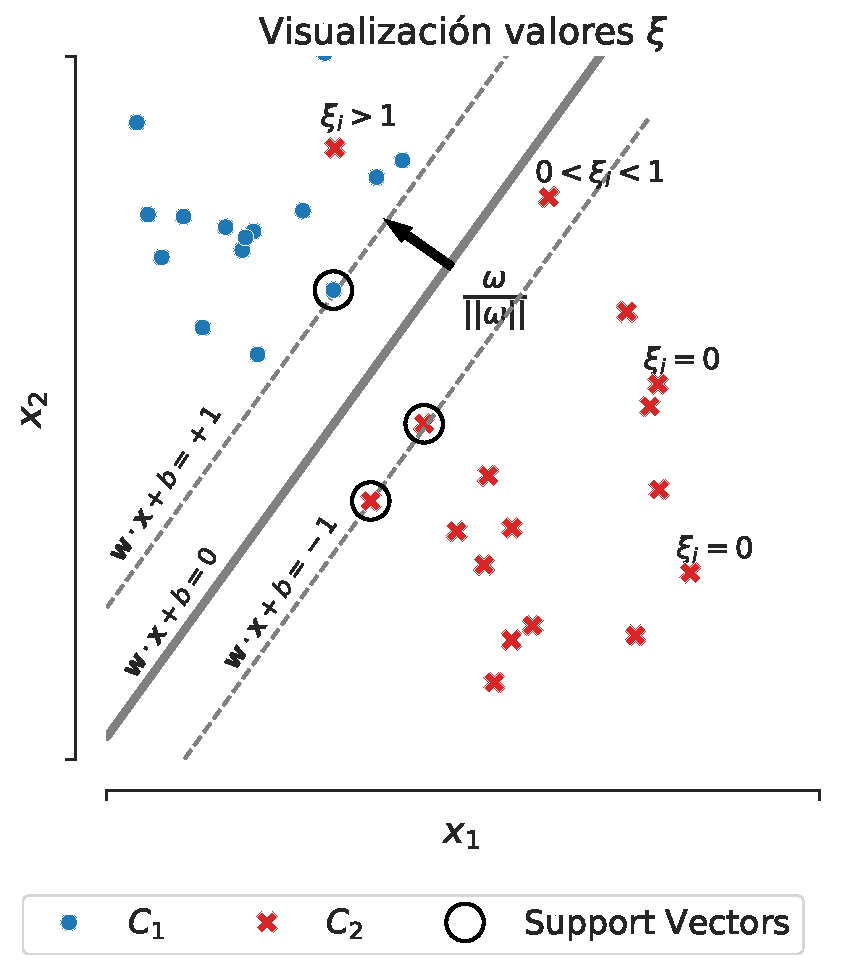
\includegraphics[width=0.45\textwidth]{img/cap5_max_margen3}
    \caption{Valores para las variables de holgura $\xi$ en distintas regiones del espacio de entrada.}
    \label{fig:soft_margin}
\end{figure}

Procediendo de la misma forma que en el caso anterior, el dual de este problema es (lagrangiano):
\begin{equation}
\begin{aligned}
(D)\quad & \underset{\alpha}{\text{max}}
& & \sum\limits_{i=1}^{N}\alpha_i - \frac{1}{2} \sum\limits_{i,j=1}^{N} \alpha_i \alpha_j y_i y_j \langle x_i, x_j\rangle\\
& \text{s.a}
& & \sum\limits_{i=1}^{N} \alpha_i y_i= 0 \\
& &  &0 \leq \alpha_i \leq c.
\end{aligned}
\end{equation}
Esta solución similar al caso anterior y también se puede resolver con técnicas de programación cuadrática, en particular, su solución también existe y es única. La diferencia entre ambas soluciones (con y sin variables de holgura) está dada por el hecho de que los multiplicadores de Lagrange ahora están acotados por el hiperparámetro $c$, el que representa la importancia que se da a la suma de las variables de holgura versus el ancho del margen en la función de costo del problema de optimización.

Por último, ¿cómo definir el parámetro $c$? Es posible responder esta pregunta en relación al \textit{bias-variance tradeoff}. Notemos que $\xi_i>1$ si la muestra $x_i$ está mal clasificada, entonces el término $\sum_{i=1}^{N} \xi_i$ es una cota superior para la cantidad de muestras mál clasificadas. Consecuentemente, el hiperparámetro $c$ es un coeficiente (\emph{inverso}) de regularización, pues su magnitud controla el balance entre la maximización del margen y la cantidad muestras mal clasificadas. En particular, para un $c$ muy alto la cantidad de muestras mal clasificadas tiene mucho peso relativo comparada contra el ancho del margen en el funcional de minimización, con lo que la solución óptima tendrá un margen muy angosto y pocas (si es que hay alguna) muestras mal clasificadas. En efecto, si $c\to\infty$, se recupera la formulación del \emph{margen duro} y su misma solución de máximo margen (en el caso de que el problema sea efectivamente linealmente separable), pues solo se podrá resolver el problema si todas las variables de holgura son nulas. Por el contrario, para un $c$ pequeño el margen tiene más importancia que la cantidad de datos incorrectamente clasificados, con lo que se encontrará un margen amplio con varias muestras mal clasificadas. Es de esperar que un $c$ pequeño (margen amplio) tenga mejor capacidad de generalizar a nuevos datos con menor varianza, mientras que un $c$ grande puede sobreajustar a los datos disponibles, reportando peor desempeño \emph{out-of-sample}. Por esto hemos dicho que $c$ es análogo a un coeficiente \emph{inverso} de regularización, pues mientras más pequeño, más regular es la solución. 

Al no conocer los estadísticos de los datos, en la práctica ajustamos el hiperparámetro $c$ mediante validación cruzada.

\subsection{Método de kernel}

El clasificador SVM (tanto con margen duro o blando) tiene una propiedad muy beneficiosa en el caso linealmente separable: la solución siempre existe, es única y se puede encontrar. Sin embargo, no tenemos ninguna garantía en los casos no separables, los cuales afloran usualmente en la práctica. Consideremos el problema de clasificar una base de datos generadas con una función ``o exclusivo'', o ``XOR'', presentada en la Fig.~\ref{fig:xor}. Estos datos no son linealmente separables, con lo que al calcular el clasificador óptimo  de SVM no llegaríamos a ninguna solución coherente ya que el problema es infactible, sin embargo, notemos que es posible diseñar una característica particular para este conjunto donde sí son separables. 

\begin{figure}[ht]
    \centering
    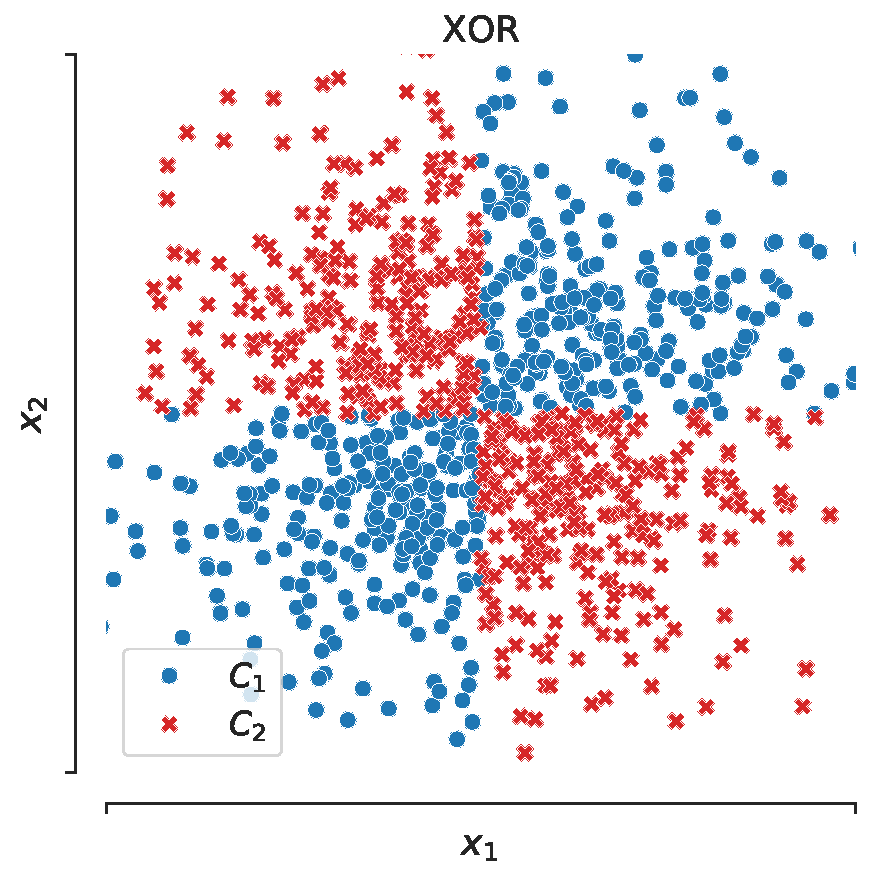
\includegraphics[width=0.45\textwidth]{img/cap5_xor}
    \caption{Datos XOR: no son linealmente separables.}
    \label{fig:xor}
\end{figure}

En efecto, consideremos el mapa desde  $\R^2$ a $\R^3$ definido mediante
\begin{equation}
    \phi: [x_1, x_2]^\top \mapsto [x_1, x_2, x_1 x_2]^\top,
\end{equation}
y observemos que éste permite clasificar de forma lineal (y trivial) las clases del problema XOR: ambas quedan clasificadas mediante el plano $z=0$ en $\R^3$, esto es ilustrado en la Fig.~\ref{fig:xor_proyectado}. La función $\phi$ es un ejemplo de una ingeniería de características como las vistas en el capítulo de regresión no lineal, en este caso particular, la característica relevante era precisamente $x_1x_2$.

\begin{figure}[ht]
    \centering
    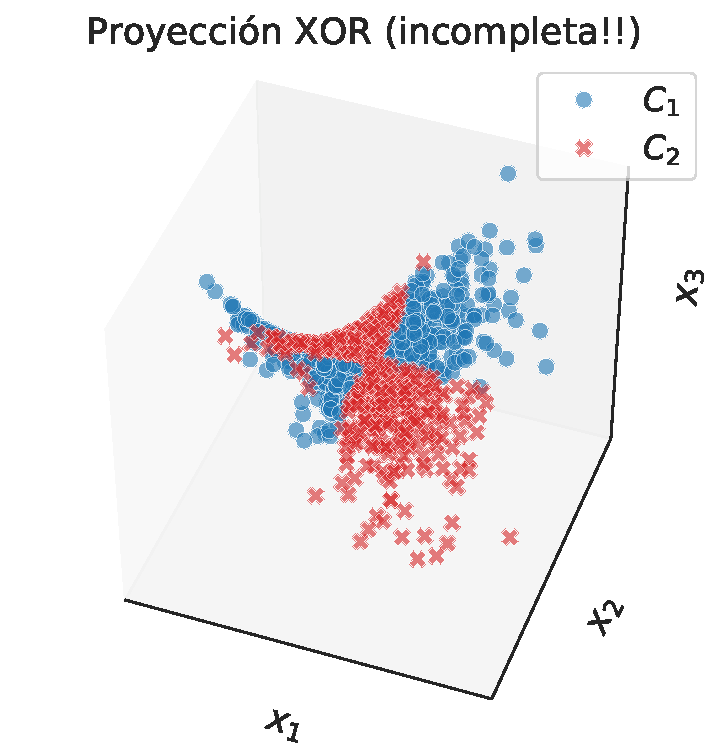
\includegraphics[width=0.45\textwidth]{img/cap5_xor_3d_proyeccion}
    \caption{Los puntos rojos y azules corresponden a los datos mapeados a través de $\phi$. El plano $z=0$ es capaz de separar puntos rojos y puntos azules en este nuevo espacio.}
    \label{fig:xor_proyectado}
\end{figure}

%%VOLVER A PROYECTAR

\begin{remark}
En el caso del problema XOR conocíamos la característica apropiada, sin embargo, en el caso general no es claro cuál debe ser ``el buen $\phi$''. A pesar de esto, notemos que tanto para la formulación con margen duro o blando de SVM, la solución solo requerirá que seamos capaces de calcular los productos internos entre las características de cada entrada. Es decir, si consideramos un $\phi$ arbitrario para nuestro problema de clasificación, solo necesitaríamos calcular los productos puntos de la forma
\begin{equation}
    \langle \phi(x_i) , \phi(x_j) \rangle, 
\end{equation}
para todo $x_i,x_j$ en el conjunto de entrenamiento. 
\end{remark}

Podemos entonces aplicar la siguiente intuición: seguramente no podemos encontrar el $\phi$ exclusivo de cada problema, sino que podemos utilizar uno (o una clase) que sea muy general, complejo, o ``universal''. Esperamos que esta característica general nos sirva para una gran cantidad de problemas, donde tenemos la garantía de que lo podremos usar como parte de SVM si somos capaces de calcular su producto interno. Además, por ``general'' podemos entender ``de alta dimensión'': podríamos pensar que para un problema en el cual no sabemos el buen $\phi$, podemos considerar incorporar e incorporar características, con lo cual tendríamos una ``característica agregada'' de alta dimensión, esperando que alguno de los términos agregados sea el que efectivamente separa las clases. Si bien no está garantizada la separabilidad lineal al combinar características, al agregar dimensiones los datos están cada vez más separados debido a la maldición de la dimensionalidad (ver anexos) y se puede probar que en dimensión infinita, siempre se podrá separar linealmente.

\begin{figure}[h]
    \centering
    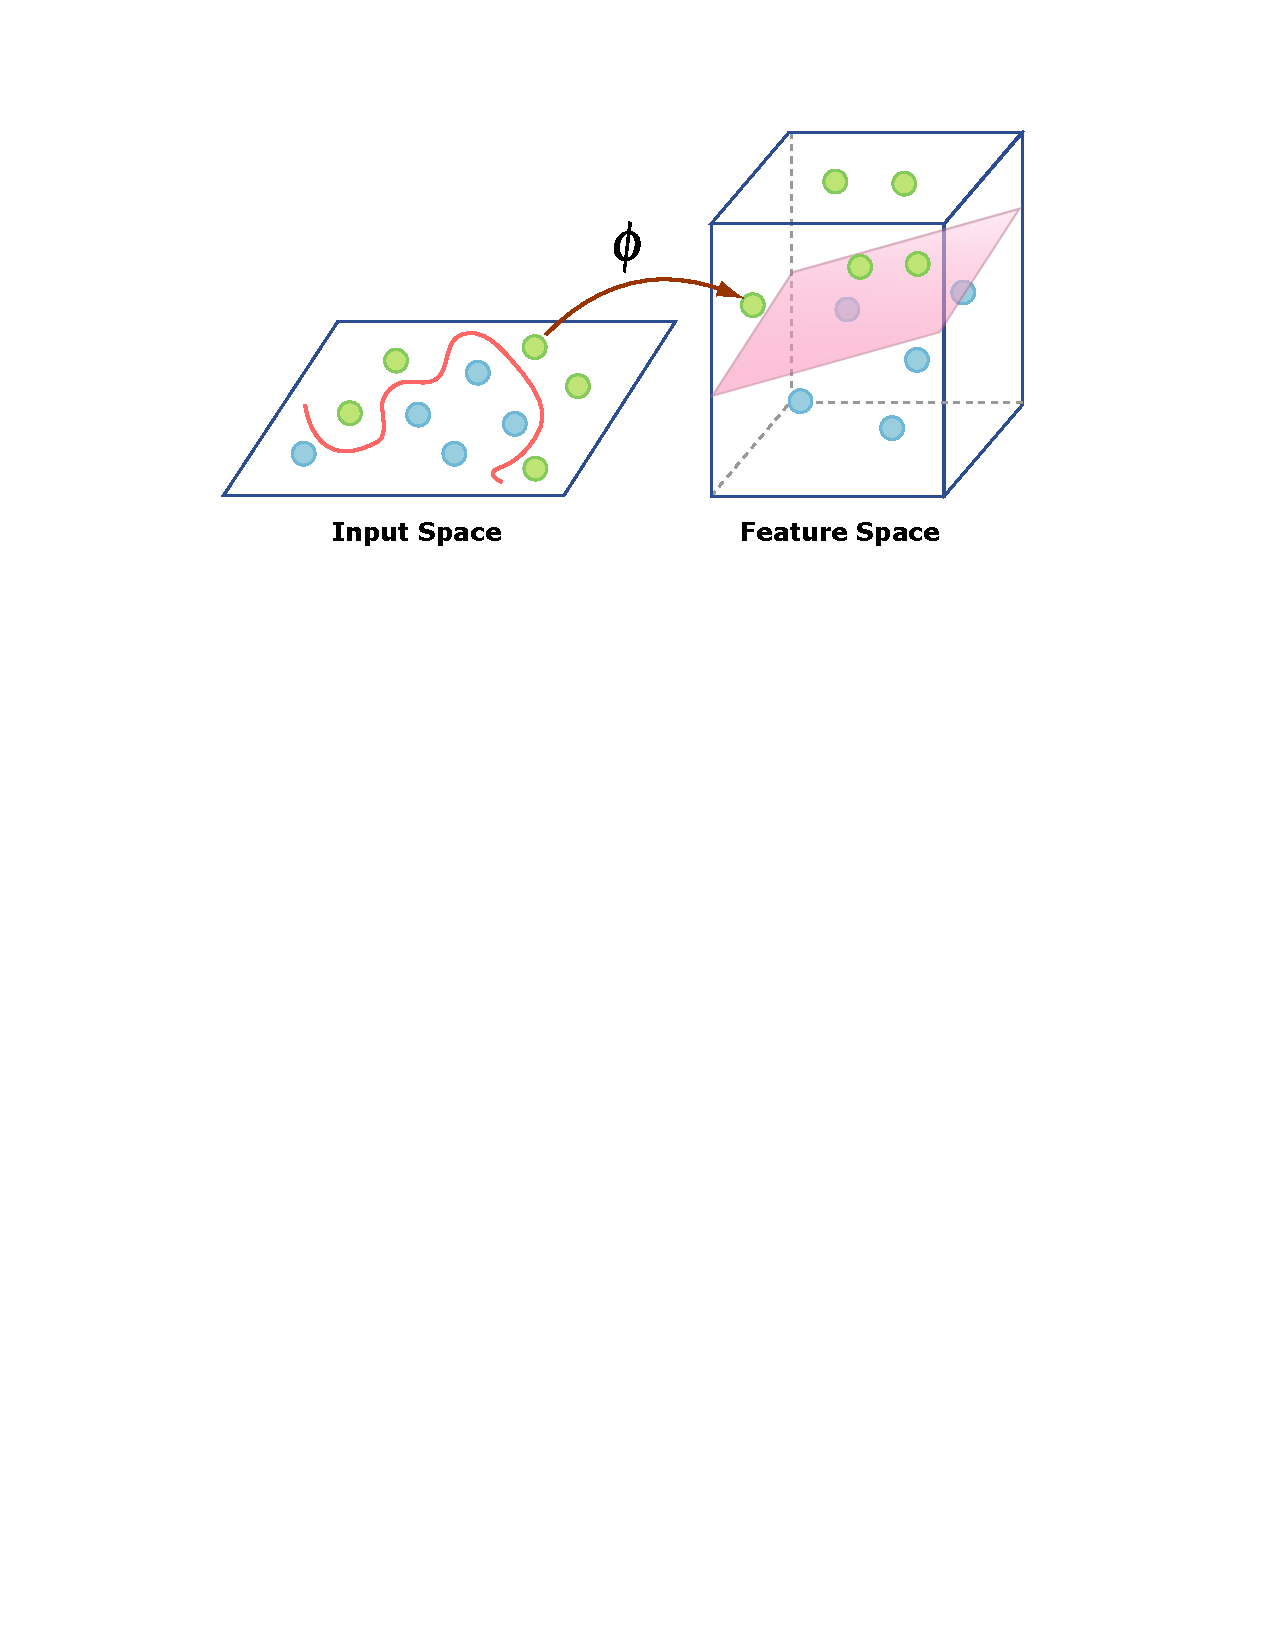
\includegraphics[width=0.45\textwidth]{img/cap5_kernelSVM}
    \caption{Separación lineal en un espacio de dimensión mayor. Imagen obtenida de MIT OpenCourseWare (MIT 15.097 course).}
\end{figure}



\newpage

Para encontrar estos $\phi$ generales, veamos la siguiente definición
\begin{definition}[Mercer kernel]
    Un Mercer kernel es una función continua $K: X\times X \to \R$ tal que
\begin{itemize}
    \item Es simétrica $K(x_1 , x_2 ) = K (x_2 , x_1)$
    \item Es definida positiva, es decir
    $$\int_{X^2} K(x_1, x_2)g(x_1) g(x_2) dx_1 dx_2\geq 0,$$
    para toda función $g:X\rightarrow\R$ continua. El nombre de de esta propiedad derivada de su similitud con las matrices definidas positivas: si $g$ se mira como vector de $\R^X$, entonces la expresión anterior representa a $g^\top Kg\leq 0$.
\end{itemize}

\end{definition}

De esta forma, se tiene el siguiente teorema de analisis funcional que sustenta la utilización de kernels en los algoritmos de aprendizaje automático:


\begin{theorem}[teorema de Mercer (simplificado)]
	Sea $K: X\times X \to \R$ un Mercer kernel, entonces existe un espacio de Hilbert $\left(\mathcal{H},\langle,\rangle\right)$ y una función $\phi: X \to \mathcal{H}$ tal que:
	\begin{equation}
    K(x_1, x_2) = \langle \phi(x_1) , \phi(x_2) \rangle
\end{equation}
\end{theorem}

Es decir, existe un mapa de características $\phi$ tal que $K(x_1, x_2)$ representa el producto interno (en algún espacio) de las características de $x_1$ y $x_2$. Además, dicho espacio no es necesariamente de dimensión finita.

\begin{remark}[truco del kernel]
La introducción del concepto de kernel es fundamental en SVM. La definición y lema anteriores nos dicen que para cualquier función simétrica y definida positiva $K$, existe una función $\phi$, que puede ser incluso de dimensión infinita, tal que la evaluación del kernel en dos puntos cualquiera equivale al producto interno entre dos evaluaciones de $\phi$ en los mismos puntos, es decir, $K(x_1,x_2)$ representa un producto interno en algún espacio de características. Esto, sumado al hecho de que la solución de SVM solo requiere del cálculo de productos internos, nos permite construir \emph{kernel SVMs}, donde parametrizamos directamente el producto interno en el problema de optimización mediante el kernel, pues esto da la garantía que el mapa de características $\phi$ existe. El caso interesante es cuando ocupamos un kernel que corresponde a un $\phi$ infinito dimensional, pues estamos efectivamente realizando la clasificación en un espacio de dimensión infinita pero con un procedimiento que solo requiere de una cantidad finita de cálculos, esto se llama \emph{el truco del kernel}. Este truco puede aplicarse a cualquier algoritmo en donde las entradas solo aparezcan en la forma de productos punto, proceso que recibe el nombre de \emph{kernelización}. 
\end{remark}

\newpage

 Veamos distintos tipos de kernels y sus propiedades.

\begin{itemize}
    \item   \textbf{Kernel polinomial:}
    \begin{equation}
       K_{pol} (x, y) = (c + x^\top y)^d
    \end{equation}
    donde $x\geq 0$ es un parámetro libre y $d\in\N$ es el orden del polinomio. Para probar que dicha función es un kernel, basta reagrupar los términos buscando formar un producto interno. Para $x,y\in\R^m$, $d=2$ se tiene que: 
    \begin{align}
        K_{pol} (x, y)  &= \left(c + \sum_{i=1}^m x_iy_i\right)^2\\
                        &= \sum_{i=1}^m (x_i^2)(y_i^2) + \sum_{i=2}^m \sum_{j=1}^{i-1} (\sqrt{2}x_ix_j)(\sqrt{2}y_iy_j) + \sum_{i=1}^m (\sqrt{2c}x_i)(\sqrt{2c}y_i) + c^2\\
                        &=\langle \phi_{pol}(x) , \phi_{pol}(y) \rangle
    \end{align}
    donde 
    \begin{equation}
        \phi_{pol}(x) = [x_1^2,\ldots,x_m^2,\sqrt{2}x_1x_2,\ldots, \sqrt{2}x_{m}x_{m-1},\sqrt{2c}x_1,\ldots,\sqrt{2c}x_m,c].
    \end{equation}
    Es decir, al usar el kernel poliomial estamos implícitamente usando un mapa de características que contiene todos los monomios de grado hasta $d=2$ (si $c>0$) o bien todos los monomios de grado igual a $d=2$ (en caso que $c=0$). Más allá de esta ilustración, esto se cumple para cualquier $d\in\N$.
    \item \textbf{Función de base radial (RBF kernel)\footnote{también conocido como kernel exponencial cuadrático o gaussiano.}:} Este kernel está definido por
    \begin{equation}
        K_{RBF} (x , y ) = \sigma^2 \exp\left(-\frac{\norm{x -y}^2}{2l^2}\right).
    \end{equation}
    El mapa de características que induce es de dimensión infinita y las fronteras que entrega son suaves (infinitamente diferenciables). Los hiperparámetros del kernel son $\sigma^2$ (controla la distancia promedio de la función con su media) y $l$ (controla la oscilación de la curva).
        
    \item \textbf{Kernel periódico:}
    \begin{equation}
       K_{per} (x , y) = \sigma^2 \exp\left(- \frac{2\sen^2 \left(\frac{\pi|x -y|}{p}\right)}{l^2}\right).
    \end{equation}
    
    Este kernel es capaz de rescatar características periódicas en los datos (controlados por el parámetro $p$). Los otros parámetros cumplen la misma función que el kernel anterior. 
    
\end{itemize}

Por último, el conjunto de kernels es cerrado bajo sumas y multiplicaciones, lu cual permite construir kernels más complejos combinando otros más simples. Esto será de gran utilidad en procesos gaussianos.

\subsection{Kernel ridge regression}

Veamos que es directo kernelizar el método de mínimos cuadrados regularizados visto en la Sección \ref{sub:min_cuad_reg}. En particular, consideremos el caso de regularización cuadrática, el cual, vimos que tiene solución
\begin{equation}
    \theta_{MCR} = \left(\tX^\top\tX +\rho \eye\right)^{-1} \tX^\top Y
    \label{eq:RR_soln1}
\end{equation}
 y consecuentemente, reporta una predicción en base a un nuevo input $x_\star$ dada por $\hat{y}_\star = \theta_{MCR}^\top x_\star$. Como podemos ver, la interacción de las entradas $(\tx_i)_{i=1}^N$ no aparece en la forma de productos internos (lo cual es necesario para la kernelización) ya que $(\tX^\top\tX)_{ij}=\langle\tX^\top_{i\cdot},\tX_{\cdot j}\rangle=\langle\tX_{\cdot i},\tX_{\cdot j}\rangle$, es decir, es el producto interno de las columnas de $\tX$ y no de los datos (recordar que $\tx_i = \tX_{i\cdot}$). Sin embargo, se tiene la siguiente propiedad de inversión:

\begin{lemma} La solución de mínimos cuadrados es equivalente a

\begin{equation}
	\theta_{MCR} = \tX^\top\left(\tX\tX^\top + \rho\eye\right)^{-1}Y
	\label{eq:RR_soln2}
\end{equation}

\end{lemma}

\begin{proof}
	Usando la fórmula de Woodburry (ver anexos)
	
	\begin{equation}
		(A+UCV)^{-1} = A^{-1} - A^{-1}U(C^{-1}+VA^{-1}U)^{-1}VA^{-1}
	\end{equation}
	
considerando $A=\rho\eye$, $U=\tX^\top$, $C=\eye$ y $V=\tX$, se tiene que:
\begin{align}
	\theta_{MCR} &= \left(\frac{1}{\rho}\eye- \frac{1}{\rho}\tX^\top\left(\eye+\frac{1}{\rho}\tX\tX^\top\right)^{-1}\frac{\tX}{\rho}\right)\tX^\top Y=\frac{1}{\rho}\tX^\top \left(\eye- \left(\eye+\frac{1}{\rho}\tX\tX^\top\right)^{-1}\frac{\tX\tX^\top}{\rho}\right)Y\\
	&= \frac{1}{\rho}\tX^\top \left(\eye- \left(\eye+\frac{1}{\rho}\tX\tX^\top\right)^{-1}\left(\eye+\frac{1}{\rho}\tX\tX^\top\right) + \left(\eye+\frac{1}{\rho}\tX\tX^\top\right)^{-1}\right)Y\\
	&= \frac{1}{p}\tX^\top\left(\eye+\frac{\tX\tX^\top}{\rho}\right)^{-1}Y= \tX^\top\left(\tX\tX^\top + \rho\eye\right)^{-1}Y
\end{align}
\end{proof}

Donde ahora $\tX\tX^\top$ sí corresponde a un producto externo de las entradas:

\begin{equation}
	(\tX\tX^\top)_{ij}=\langle\tX_{i\cdot},\tX^\top_{\cdot j}\rangle=\langle\tX_{i\cdot},\tX_{j\cdot}\rangle = \langle \tx_i,\tx_j\rangle
\end{equation}

Además,

\begin{equation}
	\hat{y}_\star = \theta_{MCR}^\top x_\star = Y^\top \left(\tX\tX^\top + \rho\eye\right)^{-1}\tX \tx_\star
\end{equation}

donde $(\tX x_\star)_i = \langle \tilde{x}_i,x_\star\rangle$, lo cual muestra que las entradas solo aparecen en la predicción en forma de productos internos.

\begin{remark}[Costo computacional: dimensión v/s cantidad de datos]
Como $\tX\in\R^{N\times M}$, donde $N$ es la cantidad de datos y $M$ es la dimensión de los datos de entrada, entonces la matriz a invertir en la ec.~\eqref{eq:RR_soln1} es de tamaño $M\times M$, mientras que la matriz a invertir en la ec.~\eqref{eq:RR_soln2} es de tamaño $N\times N$. Como el costo de invertir una matriz es de orden cúbico (dependiendo del método) en su dimensión, será preferible utilizar una de las dos formulaciones en base a qué es mayor, la dimensión o el número de datos. 
\end{remark}

Por otro lado, sea $\phi$ un mapa de características (i.e., una función que recupera las características de una entrada $x$), denotando las características por $\phi_i=\phi(x_i)$ y $\phi_\star = \phi(x_\star)$, se puede hacer la regresión sobre las características:

\begin{equation}
	\Theta=\left(\begin{matrix}
		\phi_1^\top\\
		\vdots\\
		\phi_N^\top
	\end{matrix}\right) \implies \hat{y}_\star = Y^\top \left(\Theta\Theta^\top + \rho\eye\right)^{-1}\Theta \phi_\star
\end{equation}

Luego, si $K$ es un kernel asociado al mapa de características $\phi$, es decir $K(x_i,x_j)=\langle\phi(x_i),\phi(x_j)\rangle$, se tiene que


\begin{equation}
    \hat{y}_\star = Y^\top \left(\Theta\Theta^\top + \rho\eye\right)^{-1}\Theta \phi_\star  = Y^\top \left(K(\tX,\tX) + \rho\eye\right) ^{-1} K(\tX, x_\star),    
\end{equation}

donde se ha hecho abuso de notación al usar argumentos matriciales en el kernel:
\begin{equation}
	K(\tX,\tX)_{ij} = (\Theta\Theta^\top)_{ij} = \langle\phi_i,\phi_j\rangle = K(x_i,x_j)\qquad K(\tX,x_\star)_i = (\Theta\phi_\star)_i = \langle\phi_i,\phi_\star\rangle = K(x_i,x_\star)
\end{equation}

Alternativamente, esta predicción puede ser reordenada para dar 
\begin{equation}
   \hat{y}_\star    = \sum_{i=1}^N h_i K(x_i,x_\star)\label{eq:RR_pred2},
\end{equation}
donde hemos denotado el vector $h\in\R^N$ de la forma $h_i = \left(Y^\top \left(K(\tX,\tX) + \rho\eye\right) ^{-1}\right)_i$. Hay varias observaciones relevantes que podemos hacer con respecto al resultado anterior. 

\begin{remark}[Infinitas características]
Como hemos descrito la predicción de MCR en forma de productos internos, podemos reemplazar las entradas $x$ en las descripción anterior por una característica $\phi(x)$, de dimensión $D$. Luego, si el kernel $K$ tiene asociado un mapa de dimensión infinita, la regresión se hará sobre dicho mapa, buscando separar la entrada en un espacio de dimensión infinita. 
\end{remark}


\begin{remark}[Kernel como similitud]
    Notemos de la expresión anterior que si el kernel $K(x,x')$ es una medida de similitud entre $x$ y $x'$, entonces la predicción de $y_\star$ es una combinación lineal de $h_i$, donde los ponderadores de cada $h_i$ son mayores para los datos $x_i$ que se parecen (con respecto a $K$) a la nueva entrada $x_\star$. A su vez, los valores $h_i$ son una transformación lineal de las entradas $Y$, con lo que la predicción de \emph{kernel ridge regression} combina linealmente salidas conocidas en base a cuán similar a los datos históricos es una nueva entrada. 
\end{remark}

\begin{remark}[Modelo no paramétrico] Como vimos anteriormente, el hecho de que la predicción en la ec.~\eqref{eq:RR_pred2} solo dependa del kernel permite evitar definir explícitamente el mapa de características $\phi$, sino que solo necesitamos el kernel $K$. Esto permite utilizar un kernel (e.g., exponencial cuadrático) que corresponde a un $\phi$ de dimensión infinita, lo que resulta en el parámetro $\theta$ siendo también de dimensión infinita. A pesar de la característica \emph{infinita} de este método, solo necesitamos hacer un cálculo finito para representar $\hat{y}_\star$, esto se puede interpretar como la extracción de la información suministrada por los datos que tenemos $\datos = \{x_1,\ldots,x_n\}$, los cuales son finitos a pesar de que el modelo tenga una ``capacidad'' infinita (ver el Teorema del representante). Una consecuencia de esto es que la predicción en la ec.~\eqref{eq:RR_pred2} depende de todos los elementos de $\datos$, a diferencia de todos los modelos que hemos visto hasta ahora, donde la información de los datos (independiente de cuántos fueran) quedaba resumida en un parámetro de dimensión fija. Nos referimos a este tipo de modelo (con infinitos parámetros) como \emph{no paramétricos} debido a que su tratamiento no puede ser de la misma forma que los modelos con parámetros finitos.  
\end{remark}

\begin{remark}[Complejidad variable] 
Finalmente, el hecho que los modelos no paramétricos tengan una cantidad de términos creciente en la cantidad de observaciones implica que su complejidad y desempeño son crecientes también. Esto está de acuerdo con la intuición de que  un modelo no debería tener una complejidad o capacidad fija, sino que flexible a medida que se va considerado una mayor evidencia.
\end{remark}

\subsection{Kernel SVM}

Volvamos ahora a SVM para convertir un problema no linealmente separable en uno linealmente separable (en algún espacio) mediante una \emph{kernelización}, es decir, reemplazando las entradas $x$ por un mapa de características $\phi(\cdot)$ de alta (o infinita) dimensión. Como vimos anteriormente, si la formulación de SVM está expresada en forma de productos internos (y sí que lo está), a través del truco del kernel podemos parametrizar directamente dichos productos internos con un kernel $K(\cdot,\cdot)$ sin la necesidad de definir explícitamente el mapa $\phi$. 

Reemplazando entonces las entadas por las características igual que en el caso de regresión de ridge, la kernelización del SVM con margen suave tiene una formulación primal dada por
\begin{equation}
\begin{aligned}
(P)\quad & \underset{w,b}{\text{min}}
& & \frac{1}{2}||w||^2 + c\sum\limits_{i=1}^{N} \xi_i\\
& \text{s.a}
& & y_i (w^\top \phi(x_i) +b) \geq 1- \xi_i, \; i = 1, \ldots, N.
\end{aligned}
\end{equation}
Mientras que su formulación dual tiene la forma
\begin{equation}
\begin{aligned}
(D)\quad & \underset{\alpha}{\text{max}}
& & \sum\limits_{i=1}^{N}\alpha_i - \frac{1}{2} \sum\limits_{i=1}^{N} \alpha_i \alpha_j y_i y_j \langle\phi(x_i), \phi(x_j)\rangle\\
& \text{s.a}
& & \sum\limits_{i=1}^{N} \alpha_i y_i= 0 \\
& &  &0 \leq \alpha_i \leq c.
\end{aligned}
\end{equation}
Podemos ocupar el truco del kernel para parametrizar directamente el producto interno $\langle \phi(x_i), \phi(x_j)\rangle$ mediante $K(x_i,x_j)$. Con esto, el problema de optimización en el dual se convierte en 
\begin{equation}
\begin{aligned}
& \underset{\alpha}{\text{max}}
& & \sum\limits_{i=1}^{N}\alpha_i - \frac{1}{2} \sum\limits_{i=1}^{N} \alpha_i \alpha_j y_i y_j K(x_i, x_j)\\
& \text{s.a}
& & \sum\limits_{i=1}^{N} \alpha_i y_i= 0 \\
& &  &0 \leq \alpha_i \leq c.
\end{aligned}
\end{equation}

\begin{remark}[Kernel SVM]
Esta formulación, al igual que el SVM lineal original, es un QP  con solución única, pues  el kernel $K$ es definido positivo y por ende el funcional de optimización es cuadrático y cóncavo. Consecuentemente, una vez calculadas las $N(N+1)/2$ evaluaciones de la forma $K(x_i, x_j)$, lo único que queda es resolver un problema QP.  Es particularmente relevante ver que kernel SVM tiene el mismo orden de complejidad computacional que el SVM lineal.
\end{remark}

\begin{figure}[h]
    \centering
    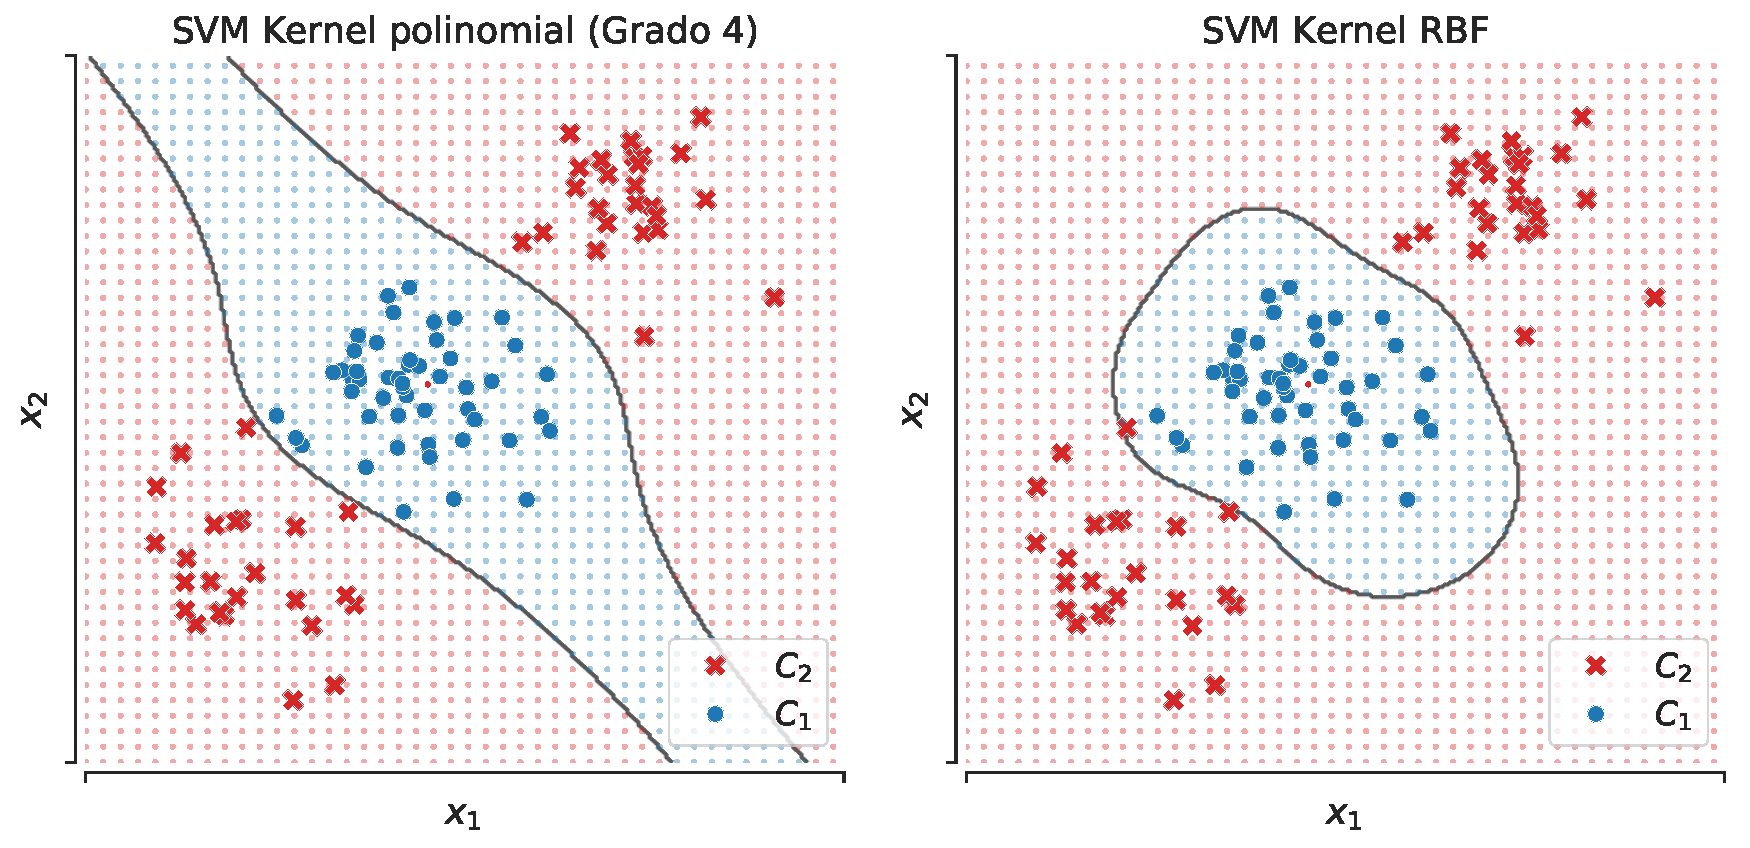
\includegraphics[width=0.75\textwidth]{img/cap5_svm_2kernels}
    \caption{Clasificación usando kernel SVM (margen suave) con distinto kernels: polinomial a la izquierda y RBF a la derecha.}
    \label{fig:ksvm}
\end{figure}

La Fig.~\ref{fig:ksvm}  muestra la implementación de kernel SVM para dos kernels: a la izquierda se ocupó un kernel polinomial de grado $3$, dicho kernel se caracteriza por su curvatura en los límites del clasificador, mientras que a la derecha se ocupó un kernel RBF, el cual es capaz de encontrar fronteras de decisión más curvadas (infinitamente diferenciables).\\

Finalmente, observemos que los métodos de kernel tienen una tremenda ventaja computacional con respecto a sus contrapartes sin kernel. Transformar los datos a un espacio de mayor dimensión  definiendo explícitamente $\phi(x)$ puede ser muy costoso, o incluso imposible, en el caso que el espacio de llegada sea infinito-dimensional. Usando kernels, por el contrario, dicha función queda implícita en el problema, y el método tiene un costo finito a pesar de que el modelo efectivamente opera en un espacio de características infinito (en el caso de RBF por ejemplo).


%-Comparar rendimiento de logistic regression c on SVM lineal
%-Usar diferentes Kernels
%-Ver el overfitting cuando ocupas un polinomio de muchos grados
%-Ver la importancia de escalar los datos

\newpage

%!TEX root = notas_de_clase.tex

\section{Procesos gaussianos}


Como se vio en capítulos anteriores, el problema de regresión busca encontrar una función $y= f(x)$, dado un conjunto de pares de la forma $\mathcal{D}=\{(x_i, y_i)\}_{i=1}^N$. Dentro de los métodos vistos para resolver el problema de regresión, se vio el de regresión lineal, lineal en los parámetros y no lineales. Una característica en común que tienen estos métodos es que el proceso de entrenamiento consiste en encontrar un número fijo de parámetros, que minimicen cierta función objetivo, donde la cantidad de parámetros y la forma del modelo es parte del diseño. A este tipo de modelos se les llama \textit{modelos paramétricos}.\\

En contraste, se encuentran los modelos \textit{no paramétricos} los cuales no tienen un número fijo de parámetros, donde pueden llegar a ser en algunos casos infinito. Un ejemplo es el algoritmo de $k$-vecinos más cercanos (KNN), donde los puntos del conjunto de entrenamiento son usados para clasificar nuevas muestras. Otro ejemplo son las máquinas de soporte vectorial (SVM) donde al entrenar se obtienen los vectores de soporte.\\

Es importante hacer la distinción entre parámetros que se aprenden y los parámetros del modelo, muchas veces llamados hiperparámetros, donde estos últimos pueden ser fijos independiente si el método es paramétrico o no paramétrico. Esto se ve en el caso de SVM donde los parámetros serían los vectores de soporte, y los hiperparámetros serían el tipo de kernel, los parámetros de dicho kernel y los demás valores elegidos de antemano que definen el tipo de modelo.\\

En este capítulo introduciremos un método no paramétrico probabilístico de regresión no lineal, llamado procesos gaussianos ($\gp$). Este modelo en vez de encontrar un candidato único de la función a estimar, define una distribución sobre funciones $\mathbb{P}(f)$, donde $f$ es una función de un espacio de entrada $\mathcal{X}$ a los reales, $f: \mathcal{X} \rightarrow \mathbb{R}$. Esto tiene la virtud de permitir cuantificar la incertidumbre puntual que existe en la predicción de nuestro modelo, la cual servirá en forma de intervalos de confianza para la distribución gaussiana.\\

Partiremos definiendo un $\gp$ como una distribución a priori sobre funciones, y mostraremos que la densidad posterior se puede encontrar de forma exacta y que esta también es un $\gp$, conservando sus propiedades.\\

Es importante notar que si $\mathcal{X}$ tiene cardinalidad infinita (por ejemplo $\mathcal{X}=\mathbb{R}$), $f$ puede ser visto como un vector infinito dimensional. Como en la práctica no podemos trabajar con un vector infinito dimensional, dados $n$ puntos $\{ x_i\}_{i=1}^{n}  \subset \mathcal{X}$, podemos definirn el vector $n$-dimensional de valores de la función evaluada en dichos puntos $f(\mathbf{x})=(f(x_1), \ldots, f(x_n))^\top$.

\begin{definition}[proceso gaussiano]
	Un proceso gaussiano ($\gp$) es una colección de variables aleatorias, tal que para cualquier subconjunto finito de puntos, estos tienen una distribución conjuntamente gaussiana.
\end{definition}

Al aplicar esta definición a nuestro caso anterior, $\pr(f)$ será un $\gp$ y para cualquier conjunto finito $\{ x_i\}_{i=1}^{n}  \subset \mathcal{X}$, la distribución de $\pr(f(\mathbf{x}))$ es Gaussiana multivariada $f(\mathbf{x})=(f(x_1), \ldots, f(x_n))^\top$). En este caso las variables aleatorias representan el valor de la función $f(x_i)$ en la posición $x_i$.\\

Un $\gp$ queda completamente caracterizado por su función de media $m(\cdot)$ y función de covarianza $K(\cdot, \cdot)$, de esta forma para cualquier conjunto finito podemos encontrar la distribución. Definimos estas funciones como
\begin{align}
	m(x) & = \mathbb{E}\left\{f(x)\right\}\\
	K(x, x') & = \mathbb{E}\left\{\left(f(x) - m(x)\right) \left(f(x') - m(x') \right)\right\}
\end{align}

Y de esta forma podemos escribir el proceso como:

\begin{equation}
	f \sim \gp(m(\cdot), K(\cdot, \cdot))
\end{equation}

Donde para un conjunto finito tenemos que la marginal resulta de la forma:

\begin{equation}
	f(\x) \sim \mathcal{N}(m(\x), K(\x, \x))
\end{equation}

Hasta el momento hemos hablado del espacio de entrada $\mathcal{X}$ como genérico, un caso común es definir los $\gp$ sobre el tiempo ($\mathbb{R}^{+}$), es decir que los $x_i$ son instantes de tiempo. Es de notar que este no es el único caso, y se podría definir sobre un espacio más general, por ejemplo $\mathbb{R}^d$.\\

Otro punto a notar es que como estamos hablando de una colección (no necesariamente finita) de variables aleatorias, es necesario que se cumpla la propiedad de marginalización (o llamada consistencia\footnote{Para más detalles puede ver el teorema de consistencia de Kolmogorov}). Esta propiedad se refiere a que si un $\gp$ define una distribución multivariada para digamos dos variables $(y_1, y_2) \sim \mathcal{N}(\mu, \Sigma)$ entonces también debe definir $y_1 \sim \mathcal{N}(\mu_1, \Sigma_{11})$ donde $\mu_1$ es la componente respectiva del vector $\mu$ y $\Sigma_{11}$ la submatriz correspondiente de $\Sigma$. En otras palabras, el tomar un subconjunto más grande de puntos no cambia la distribución de un subconjunto más pequeño. Y podemos notar que esta condición se cumple si tomamos la función de covarianza definida anteriormente.

\subsection{Muestreo de un prior \texorpdfstring{$\gp$}{GP}}

Como fue mencionado, un $\gp$ define un \textit{prior} sobre funciones, por lo que, antes de ver ningún dato se podría obtener una muestra de este proceso dado una función de media y covarianza. Un supuesto común es asumir la función de media $m(\cdot)=0$ por lo que solo nos queda definir una función de covarianza o kernel, un ejemplo de kernel es el \textit{Exponencial Cuadrático} (Square Exponential), también conocido como RBF (Radial Basis function) o Kernel Gaussiano (en general se evita este nombre porque este kernel no tiene relación con la distribución de los datos).

\begin{equation}
	K_{SE}(x, x') = \sigma^2 \exp\left( - \frac{\left( x- x'\right)^2}{2\ell^2} \right)
\end{equation}

Donde en este caso los parámetros son interpretables (y como veremos más adelante pueden ser aprendidos a través de un conjunto de entrenamiento) donde $\sigma^2$ es la varianza de la función, notar que esta es la diagonal de la matriz covarianza. El parámetro $\ell$ es conocido como el \textit{lenghtscale} que determina que tan lejos tiene influencia un punto sobre otro, donde en general un punto no tendrá influencia más allá de $\ell$ unidades alrededor.\\

Como sabemos, las funciones definidas por el $\gp$ son vectores infinito dimensionales, por lo que no podemos muestrear de toda la función, pero tomando una cantidad suficiente de puntos podemos graficar muestras de un $\gp$ dada una función de covarianza. Tomando un $\gp$ con media cero ($m(\cdot)=0$) y kernel SE, muestras del proceso para distintos valores de $\ell$ obtenemos la Fig.\ref{fig:gp_1}, donde el área sombreada corresponde al intervalo de confianza del $95\%$. Se puede ver que el parámetro $\ell$ controla que tan erráticas son las funciones, donde a medida que va a aumentando las muestras se vuelven funciones más suaves.

\begin{figure}[H]
	\centering
	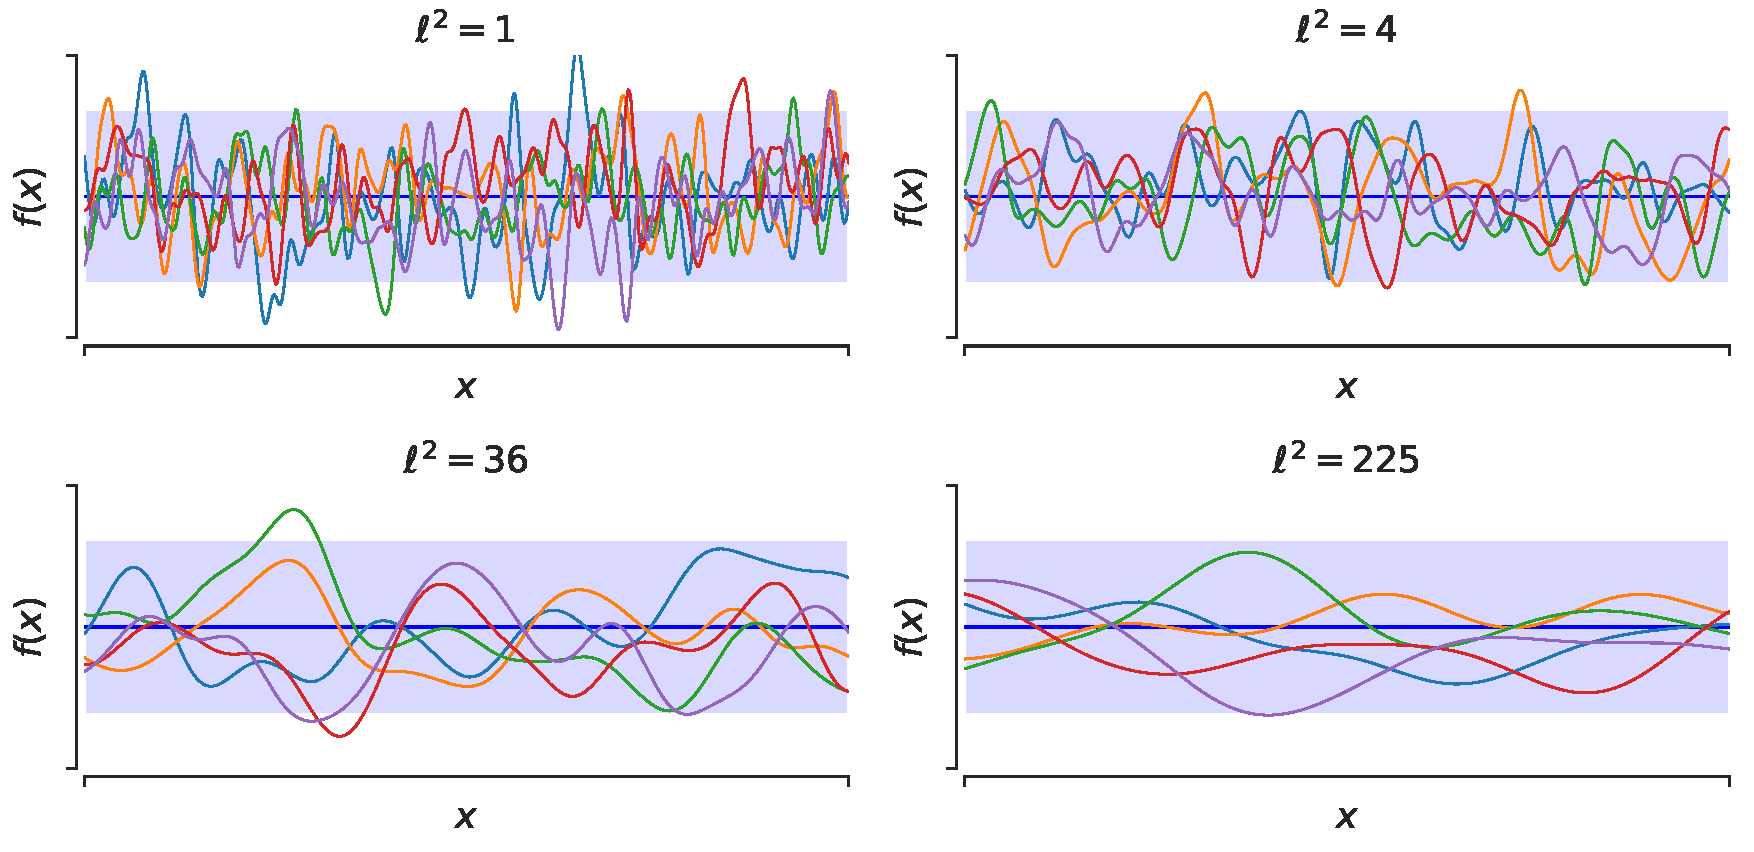
\includegraphics[width=0.9\textwidth]{img/cap8_prior_muestras}
	\caption{Muestras de un prior $\gp$ con kernel SE, para distintos \textit{lenghtscales} ($\ell$) y función media $m(\cdot)=0$, la parte sombreada corresponde al intervalo de confianza del $95\%$. Se puede ver que a mayor $\ell$ las funciones se van volviendo más suaves.}
	\label{fig:gp_1}
\end{figure}

\subsection{Incorporando información}

Ahora que ya podemos muestrear de nuestro prior, nos interesaría incorporar las observaciones que tenemos de la función a nuestro modelo. Para esto, se pueden considerar dos casos: observaciones con ruido y observaciones sin ruidos (o deterministas).

\subsubsection{Evaluación sin ruido}

 En el caso de las observaciones sin ruido, tenemos observaciones de la forma $\{(x_i, f(x_i))\}_{i=1}^{n}$, donde tenemos el valor real de nuestra función en los puntos $[x_1, \ldots, x_n]=X$. Luego, tenemos el par de entradas y observaciones $(X,f(X))$. Digamos que queremos realizar una predicción en el conjunto $X_*$ de $n_*$ puntos, luego la distribución conjunta es de la forma:
\begin{align}
	\begin{bmatrix} f(X) \\ f(X_*)  \end{bmatrix}
	\sim \mathcal{N} \left(
	\begin{bmatrix} m(X) \\ m(X_*)  \end{bmatrix}, 
	\begin{bmatrix}
		K(X, X) & K(X, X_*) \\ K(X_*, X) & K(X_*, X_*)
	\end{bmatrix}
	 \right)
\end{align}

Donde la submatriz $K(X, X_*)$ es de $n \times n_*$, $K(X, X)$ de $n \times n$ y así respectivamente para cada submatriz. Dada las observaciones y una función de covarianza, podemos evaluar la verosimilitud, que también es gaussiana, lo que nos lleva a un punto clave de los processos gaussianos:

\begin{lemma}
	Dado un prior $\gp$ sobre $f(\cdot)$ y una verosimilitud Gaussiana, la posterior sobre $f(\cdot)$ es también un $\gp$. Además, se puede condicionar sobre las observaciones $(X, f(X))$ para obtener

\begin{equation}
	f(X_*)|f(X), X  \sim \mathcal{N}(m_{X_*|X}, \Sigma_{X_*|X}) \label{eq:gp_post}
\end{equation}

Donde la media y covarianza son:
\begin{align}
	m_{X_*|X} & = m(X_*) + K(X_*, X)K^{-1}(X, X) (f(X) - m(X))\\
	 \Sigma_{X_*|X} & = K(X_*, X_*) - K(X_*, X)K^{-1}(X, X) K(X, X_*)
\end{align}
\end{lemma}

Ahora, dado un conjunto de observaciones y dada una función de covarianza, podemos obtener la densidad posterior. Para mostrar esto tomemos el caso de hacer regresión para una función conocida, para la cual tenemos observaciones sin ruido muestreadas no uniformemente, con estas observaciones queremos encontrar la función real de las que provienen; para esto usamos un prior $\gp$ con función media nula y kernel SE (por el momento tendrá parámetros fijos), nos damos un rango donde queremos hacer predicción y condicionamos en las observaciones usando la Ec.(\ref{eq:gp_post}). En este caso las observaciones corresponden al 15$\%$ de los puntos generados por nuestra función sintética.\\

Esto se muestra en la Fig.\ref{fig:gp_2}, donde podemos ver que la media de la posterior pasa por las observaciones sin incertidumbre asociada, es decir que para estos puntos se tiene una posterior degenerada pues no hay varianza. Se puede ver que a medida que la predicción se aleja de las observaciones el intervalo de confianza (al que lo podemos asociar con incertidumbre del modelo) va creciendo.

\begin{figure}[H]
	\centering
	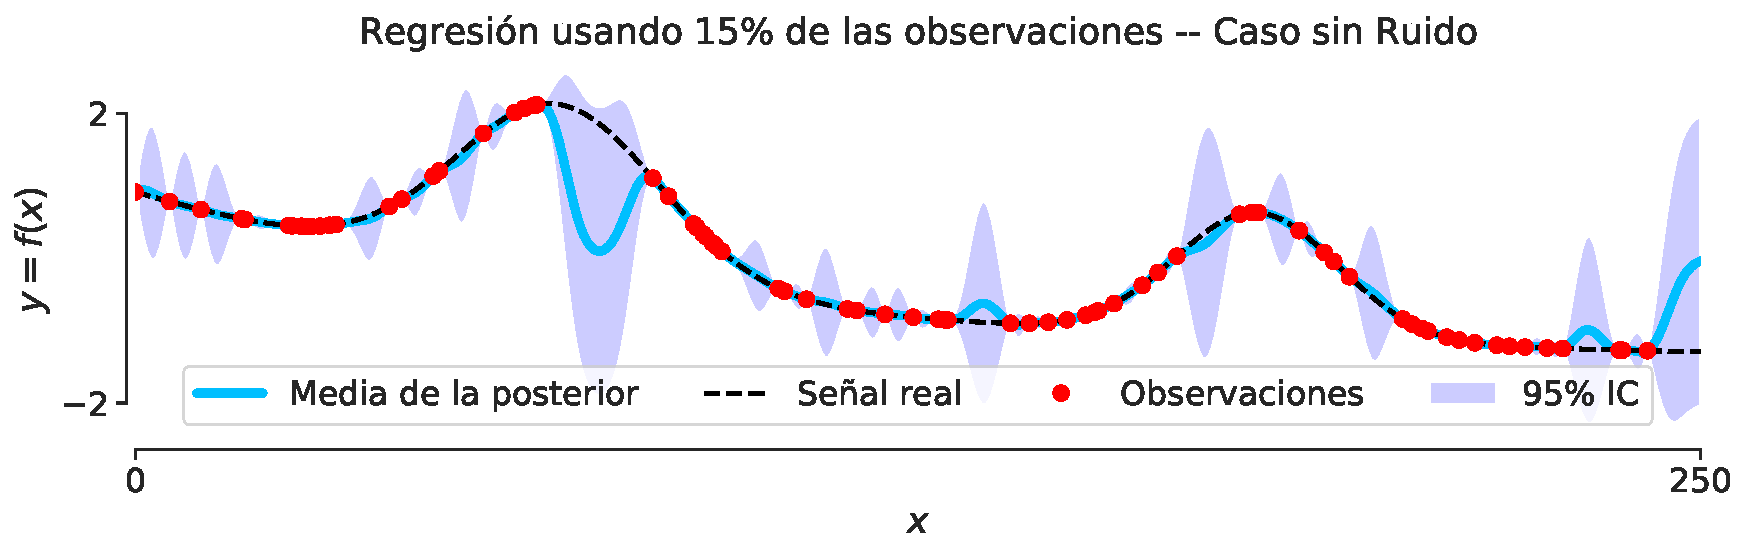
\includegraphics[width=0.9\textwidth]{img/cap8_posterior_no_ruido}
	\caption{Regresión con $\gp$ para señal sintetica usando el 15$\%$ de los datos muestreados de forma no uniforme, utilizand un $\gp$ de media nula y kernel SE.} 
	\label{fig:gp_2}
\end{figure}

\subsubsection{Evaluación con ruido}

En aplicaciones reales el caso de tener observaciones sin ruido es poco habitual, por lo que si queremos incorporar la incertidumbre real debemos tomar en cuenta errores de medición en nuestro modelo. Tomemos el caso de tener observaciones contaminadas con ruido i.i.d (independientes idénticamente distribuidas) donde las observaciones serán de la forma $y_i = f(x_i) + \eta$ donde $\eta \sim \mathcal{N}(0, \sigma_n^2)$, por lo que ahora nuestro conjunto de observaciones es de la forma $(X,Y)$ donde $Y=f(X) + \eta$.

Lo que en nuestro modelo equivale a agregar un término a la función de covarianza

\begin{equation}
	cov(Y) = K(X, X) + \sigma_n^2\eye
\end{equation}

Donde si tenemos el mismo caso anterior, observaciones $(X,Y)$ y queremos evaluar en $X_*$, la conjunta queda
\begin{align}
	\begin{bmatrix} Y \\ f(X_*)  \end{bmatrix}
	\sim \mathcal{N} \left(
	\begin{bmatrix} m(X) \\ m(X_*)  \end{bmatrix}, 
	\begin{bmatrix}
		K(X,X) + \sigma_n^2 \eye & K(X, X_*) \\ K(X_*,X) & K(X_*,X_*)
	\end{bmatrix}
	 \right)
\end{align}

Notemos que el termino de ruido solo es agregado al subbloque correspondiente a las observaciones, no se agrega el termino en los otros subbloques pues buscamos hacer una predicción de la función latente $f(\cdot)$ y no una versión ruidosa de esta.
Igual que en el caso sin ruido, podemos condicionar esta conjunta a las observaciones y obtenemos el siguiente resultado:

\begin{lemma}
	Para una evaluación con ruido se tiene que
	
	\begin{equation}
		f(X_*)|Y, X  \sim \mathcal{N}(m_{X_*|X}, \Sigma_{X_*|X})\label{eq:gp_posterior}
	\end{equation}
	Donde la media y covarianza son:
	\begin{align}
		m_{X_*|X} & = m(X_*) + K(X_*, X) [K(X, X) + \sigma_n^2 \eye]^{-1} (Y - m(X))\\
	 \Sigma_{X_*|X} & = K(X_*, X_*) - K(X_*, X) [K(X, X) + \sigma_n^2 \eye]^{-1} K(X, X_*)
	\end{align}
\end{lemma}

Si tomamos el mismo ejemplo anterior, pero añadimos el ruido al modelo, obtenemos la predicción de la Fig.\ref{fig:gp_3}. En este caso podemos ver que la media de la posterior no necesariamente coincide su valor con el de la observación, pues se toma en cuenta la incertidumbre en las observaciones mismas, también se ve que no se obtienen soluciones degeneradas incluso en zonas donde hay observaciones aglomeradas.


\begin{figure}[H]
	\centering
	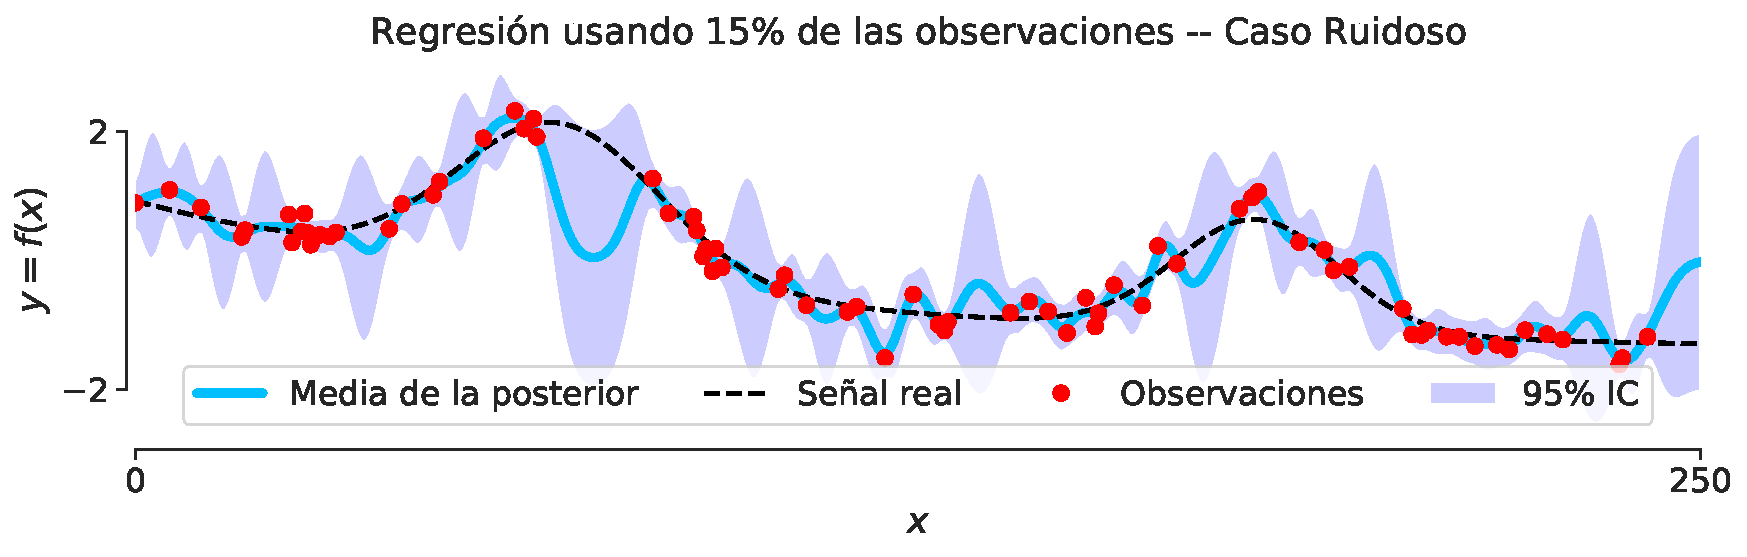
\includegraphics[width=0.9\textwidth]{img/cap8_posterior_ruido}
	\caption{Regresión con $\gp$ para señal sintetica usando el 15$\%$ de los datos muestreados de forma no uniforme y contaminados con ruido Gaussiano, utilizando un $\gp$ de media nula y kernel SE.}
	\label{fig:gp_3}
\end{figure}

\subsection{Entrenamiento y optimización de un \texorpdfstring{$\gp$}{GP}}

hasta el momento nos hemos dado la función de covarianza y sus parámetros, por lo que aún no hemos hecho realizado el \textit{aprendizaje} de nuestro $\gp$, que es lo que haremos a continuación.

\subsubsection{¿Qué es entrenar un \texorpdfstring{$\gp$}{GP}?}

Vimos que dada una función de covarianza podemos representar el proceso, y podemos encontrar analíticamente la densidad posterior de nuestra función $f(\cdot)$ condicionando a las observaciones. Pero la forma que tendrá la posterior y la función fuera de las observaciones dependerá fuertemente en nuestra función kernel escogida, en este sentido, para un kernel dado nos gustaría encontrar los parámetros de este que mejor representen nuestra función a estimar.\\

Nos referiremos a entrenar u optimizar un $\gp$ cuando queremos obtener los hyperparámetros, es decir los parámetros del kernel (los denotamos $\theta$) y la varianza del ruido (la denotamos $\sigma_n^2$) si es que aplica.

Para esto nos gustaría poder comparar funciones de covarianza, o mejor aún un funcional que podamos optimizar, afortunadamente podemos usar la \textit{verosimilitud marginal}, obtenida marginalizando sobre la función $f(\cdot)$, donde dado un conjunto de entrenamiento $(X, Y)= \{(x_i, y_i)\}_{i=1}^{n}$, esta dada por

\begin{align}
	\pr(Y|X, \theta, \sigma) & = \int \pr(Y|f, X, \theta, \sigma_n) p(f|X,\theta, \sigma) df \\
	& = \frac{1}{\left( 2\pi |\mathbf{K}_y|\right)^{\frac{n}{2}}} 
	\exp \left(
	-\frac{1}{2} (Y - \mathbf{m})^T \mathbf{K}_y^{-1} (Y - \mathbf{m})
	\right)
\end{align}

Donde $\mathbf{m}=m(X)$ y $\mathbf{K}_y=K_{\theta}(X,X) + \sigma_n^2 \eye$, la matriz de covarianza dados los parámetros $\theta$ agregando el término de la diagonal correspondiente al ruido. De la misma forma que lo hacemos con otros modelos probabilísticos, en vez de maximizar la verosimilitud, en conveniente minimizar la log-verosimilitud negativa (NLL) dada por la expresión:

\begin{align}
	NLL & = -\log \pr(Y|X, \theta, \sigma_n) \\
	NLL & = \underbrace{ \color{black}{\frac{1}{2}\log|\mathbf{K_y}|} }_
	    {\text{\parbox{2cm}{\centering Penalización\\[-4pt] por\\[-4pt] complejidad}}}
	    + \underbrace{ \color{black}{\frac{1}{2}(Y - \mathbf{m})^T \mathbf{K}_y^{-1} (Y - \mathbf{m}) }}_
	    {\text{\parbox{4cm}{\centering Data fit (Única parte que depende de $Y$)}}}
	    + \underbrace{ \color{black}{\frac{n}{2} \log2\pi}}_
	    {\text{\parbox{2cm}{\centering Constante de normalización}}}\label{eq:gp_nll}
\end{align}

De izquierda a derecha, el primer término tiene el rol de penalizar por la complejidad del modelo, y vemos que depende solo del kernel y las entradas; el segundo término cuantifica que tan bien se ajusta el modelo a los datos, y es la única componente que depende de las observaciones $Y$ (ruidosas) de la función, el último término es una constante de normalización.\\


\begin{figure}[H]
	\centering
	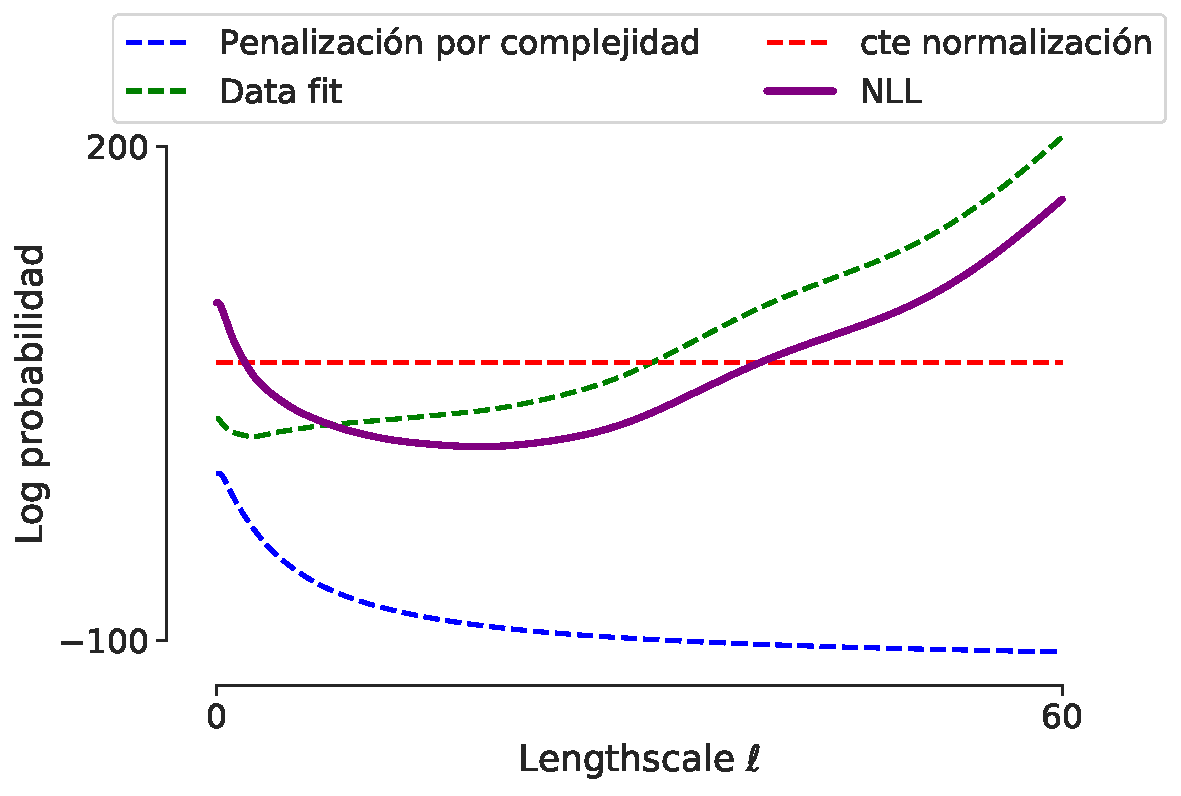
\includegraphics[width=0.5\textwidth]{img/cap8_nll_partes}
	\caption{Log verosimilitud marginal negativa (NLL) en función del \textit{lengthscale} ($\ell$) para señal sintetica, se mantienen constantes los otros parámetros del $\gp$.}\label{fig:gp_4}
	\label{fig:nll_por partes}
\end{figure}

Siguiendo con los ejemplos anteriores, para el mismo conjunto de observaciones ruidosas, se calculan las tres componentes de la $NLL$, utilizando un kernel SE, para este caso, se dejan fijo tanto la varianza de la señal como la varianza del ruido y se varia el \textit{lengthscale} $\ell$ del kernel, en la Fig.\ref{fig:gp_4}.

Al ir variando $\ell$ se ve que la penalización por complejidad va disminuyendo, pues a mayor $\ell$ menos complejas son las funciones (recordar Fig.\ref{fig:gp_1}, a mayor $\ell$ más suaves y regulares las muestras), también vemos que la componente del ajuste de datos comienza a decaer y luego se mantiene en incremento, pues a mayor \textit{lengthscale} el modelo se vuelve menos flexible, por lo que no es capaz de ajustarse de manera correcta a los datos. De esta forma, el proceso de entrenamiento dará preferencia a funciones que se ajusten bien a los datos sin ser tan complejas, ahora viendo el valor total del NLL vemos que este alcanza su mínimo en $\ell$ en el rango de $[10-30]$.\\


Ya tenemos una noción de que es entrenar un $\gp$, queremos minimizar la $NLL$ (Ec.(\ref{eq:gp_nll})) y encontrar los parámetros del kernel y del ruido (si aplica). Ahora discutiremos formas de optimizar este funcional.

\subsubsection{¿Cómo se entrena un \gp?}

Como contamos con una expresión cerrada para la NLL, podemos utilizar métodos clásicos de optimización, una opción es calcular el gradiente de esta función objetivo y aplicar algún método basado en gradiente, como L-BFGS; otra es utilizar el método de Powell que no requiere que la función sea diferenciable, por lo que no utiliza gradiente.\\


Siguiendo ejemplos anteriores, usando la misma señal sintética y las mismas observaciones ruidosas de la Fig.\ref{fig:gp_3}, ahora optimizamos nuestro $\gp$ utilizando L-BFGS, lo que nos entrega como resultado el mostrado en la Tabla.\ref{tab:gp_1} donde comparamos los parámetros del $\gp$ sin entrenar usado en la Fig.\ref{fig:gp_3}, podemos ver que no difiere mucho en cuanto a las varianzas, pues como es una señal sintética poseíamos control sobre la varianza del ruido, el valor obtenido luego de optimizar es cercano al valor real (0.2), vemos que el \textit{lengthscale} óptimo es concordante con lo analizado en la Fig.\ref{fig:gp_4}.

Por último, podemos ver la predicción usando este $\gp$ optimizado en la Fig.\ref{fig:gp_5} donde vemos que se tiene una del proceso más concordante con la función real, esto se ve especialmente en la zona con pocas observaciones, entre 50 y 100 para $x$, donde el $\gp$ sin entrenar presentaba mucha incertidumbre en esa zona, en cuanto ahora se tiene un intervalo de confianza más bien limitado pues la señal no era muy compleja.

\begin{table}[H]
\centering
\begin{tabular}{lcccc}
 & $\sigma_{\text{ruido}}$ & $\ell$ & $\sigma_{\text{señal}}$ & NLL\\ \hline
Sin entrenar & 0.2 & 3.1622 & 1 & $\mathbf{55.3538}$\\
Entrenado & 0.2067 & 18.7267 & 0.9956 & $\mathbf{17.6945}$\\
\end{tabular}
\caption{Resultado optimización $\gp$ y comparación con los parámetros sin entrenar.}
\label{tab:gp_1}
\end{table}


\begin{figure}[H]
	\centering
	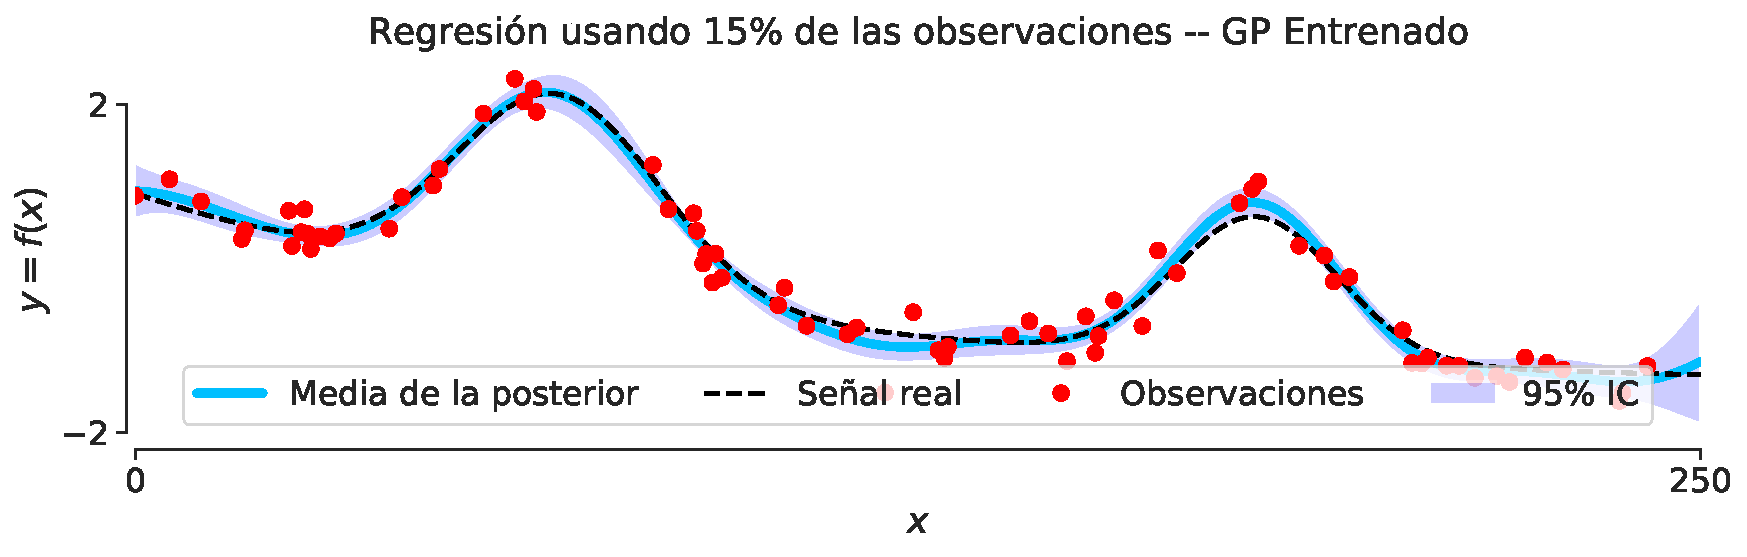
\includegraphics[width=0.9\textwidth]{img/cap8_entrenado}
	\caption{Regresión con $\gp$ para señal sintetica usando el 15$\%$ de los datos muestreados de forma no uniforme y contaminados con ruido Gaussiano, utilizando un $\gp$ de media nula y kernel SE; Modelo optimizado utilizando L-BFGS.}
	\label{fig:gp_5}
\end{figure}

La desventaja de utilizar métodos tradicionales de optimización es que estos entregan una solución puntual (en el sentido de un valor para cada parámetro, el $\gp$ sigue siendo una distribución sobre funciones), en distintas aplicaciones puede que un valor fijo de parámetros no represente de manera idónea el proceso latente a estudiar. Una opción sería computar la densidad posterior de los parámetros del kernel condicionado a las observaciones. Lamentablemente en la mayoría de los casos no existe una expresión cerrada para esta posterior, por lo que debemos recurrir a métodos de \textit{inferencia aproximada} como Markov Chain Monte Carlo (MCMC) o Inferencia Variacional.




% \subsubsection{Métricas de evaluación}
% ---pendiente---

\subsubsection{Complejidad computacional}

Es importante reconocer una de las principales desventajas de utilizar un $\gp$ cuando se cuenta con una gran cantidad de datos, esto es, su costo computacional.
Recordando, cuando queremos entrenar nuestro $\gp$ vamos a minimizar la log verosimilitud marginal negativa (NLL), mostrada en la Ec.(\ref{eq:gp_nll}), donde al observar en segundo término vemos que es la operación más costosa siendo $\mathcal{O}(n^3)$ con respecto al número de puntos de entrenamiento $n$. Hay que tomar en cuenta que la evaluación de la NLL se debe hacer en cada iteración del método de optimización elegido.

En cuanto a la evaluación, esta está dada por la Ec.(\ref{eq:gp_posterior}), donde en este caso vemos que es de orden cuadrático $\mathcal{O}(n^2)$ con respecto al número de puntos de test. Es de notar que esta vez no tomamos en cuenta la inversa de la matriz de Gram del conjunto de entrenamiento, pues puede ser precalculada y ser usada para múltiples conjuntos de test.\\

Lo anterior mencionado limita la cantidad de problemas que se pueden abordar usando estos procesos, sin embargo existen formas de obtener aproximaciones que siguen manteniendo la estructura y deseables propiedades de los $\gp$ a un menor costo computacional, estos reducen el orden de $\mathcal{O}(n^3)$ a $\mathcal{O}(nm^2)$ en entrenamiento y $\mathcal{O}(m^2)$ en test, con $m<n$. Un ejemplo de estos son los \textit{Sparse Gaussian Processes} que utilizan una aproximación de rango bajo para la matriz de covarianza, utilizando \textit{pseudo-inputs} en vez el conjunto de entrenamiento completo.


\subsection{Funciones de covarianza (kernels)}

Una función de covarianza es una función de dos argumentos donde cualquier matriz que se obtiene como resultado en la evaluación de un conjunto de puntos (la llamaremos matriz de Gram) es semidefinida positiva.

Hasta el momento solo hemos utilizado un tipo de función de covarianza, el llamado kernel \textit{Squared Exponential} (SE), conocido también como kernel RBF, dado por la Ec.(\ref{eq:gp_kernel_se}). En esta sección mostraremos distintos tipos de funciones de covarianza y los distintos tipos de funciones que generan.

\begin{equation}\label{eq:gp_kernel_se}
	K_{SE}(x, x') = \sigma^2 \exp\left( - \frac{\left( x- x'\right)^2}{2\ell^2} \right)
\end{equation}

Es importante denotar tipos de familias de funciones de covarianza, si la función solo depende de la diferencia, es decir $k(x, x')=k(x-x')$ se le llamará \textit{kernel estacionario}, más aún, si depende solo de la norma de la diferencia $k(x, x')=k(|x-x'|)$ se le llamará \textit{kernel isométrico}, un ejemplo de esto es el kernel SE.\\

Es de notar que kernels estacionarios hacen que la covarianza entre puntos sea invariante a traslaciones en el espacio de entradas. Una noción importante es que un kernel puede ser visto como una medida de similaridad entre puntos, y en el caso de kernels estacionarios, mientras más cercanos estén dos puntos más símiles serán.

\subsubsection{Rational Quadratic (RQ)}

Este kernel viene dado por la Ec.(\ref{eq:gp_kernel_rq}), este puede ser interpretado como una suma infinita de kernels SE con distintos \textit{lenghtscale}, donde $\alpha$ es un parámetro de variación de escala, notar que cuando $\alpha \rightarrow \infty$ el kernel tiende a uno SE. En la Fig.\ref{fig:gp_6} se muestra el kernel RQ, a la izquierda se ve el valor de la covarianza en función de la diferencia de los argumentos $x-x'$, a la derecha se muestran diferentes muestras de funciones con este kernel.
 
\begin{equation}\label{eq:gp_kernel_rq}
	K_{RQ}(x, x') = \sigma^2 \left(1 + \frac{\left( x- x'\right)^2}{2\alpha\ell^2 } \right)^{-\alpha}
\end{equation}


\begin{figure}[H]
	\centering
	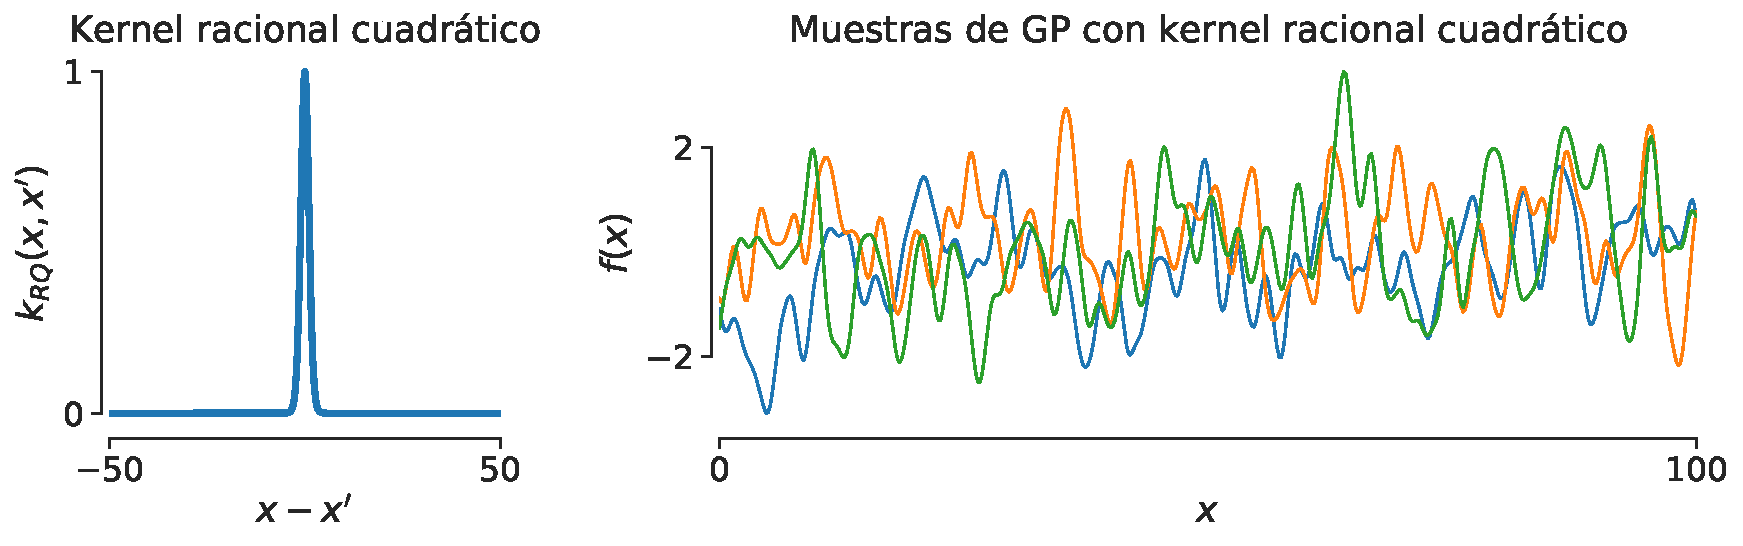
\includegraphics[width=0.9\textwidth]{img/cap8_muestras_RQ}
	\caption{Kernel \textit{Rational Quadratic}, en la izquierda se muestra la covarianza en función de su argumento $\tau=x-x'$, a la derecha de un $\gp$ usando un kernel RQ.}
	\label{fig:gp_6}
\end{figure}

\subsubsection{Kernel periódico}

Como su nombre lo indica, este kernel, dado por la Ec.(\ref{eq:gp_kernel_p}), permite modelar funciones periódicas, donde el parámetro $p$ controla el periodo de la función. Una extensión de este el kernel localmente periódico, dado por la Ec.(\ref{eq:gp_kernel_lp}) que es un kernel SE ponderado por uno periódico, este da la libertad de tener funciones con una estructura periódica local.


\begin{equation}\label{eq:gp_kernel_p}
	K_{P}(x, x') = \sigma^2 \exp\left(-\frac{2\sin^2\left(\pi |x- x'| / p \right)}{\ell^2 } \right)
\end{equation}

\begin{equation}\label{eq:gp_kernel_lp}
	K_{LP}(x, x') = \sigma^2  \exp\left(-\frac{\left(x- x' \right)^2}{2\ell^2 } \right) \exp\left(-\frac{2\sin^2\left(\pi |x- x'| / p \right)}{\ell^2 } \right)
\end{equation}

En la Fig.\ref{fig:gp_7} se muestra el kernel periódico, a la izquierda se ve el valor de la covarianza en función de la diferencia de los argumentos $x-x'$, a la derecha se muestran diferentes muestras de funciones con este kernel.

\begin{figure}[H]
	\centering
	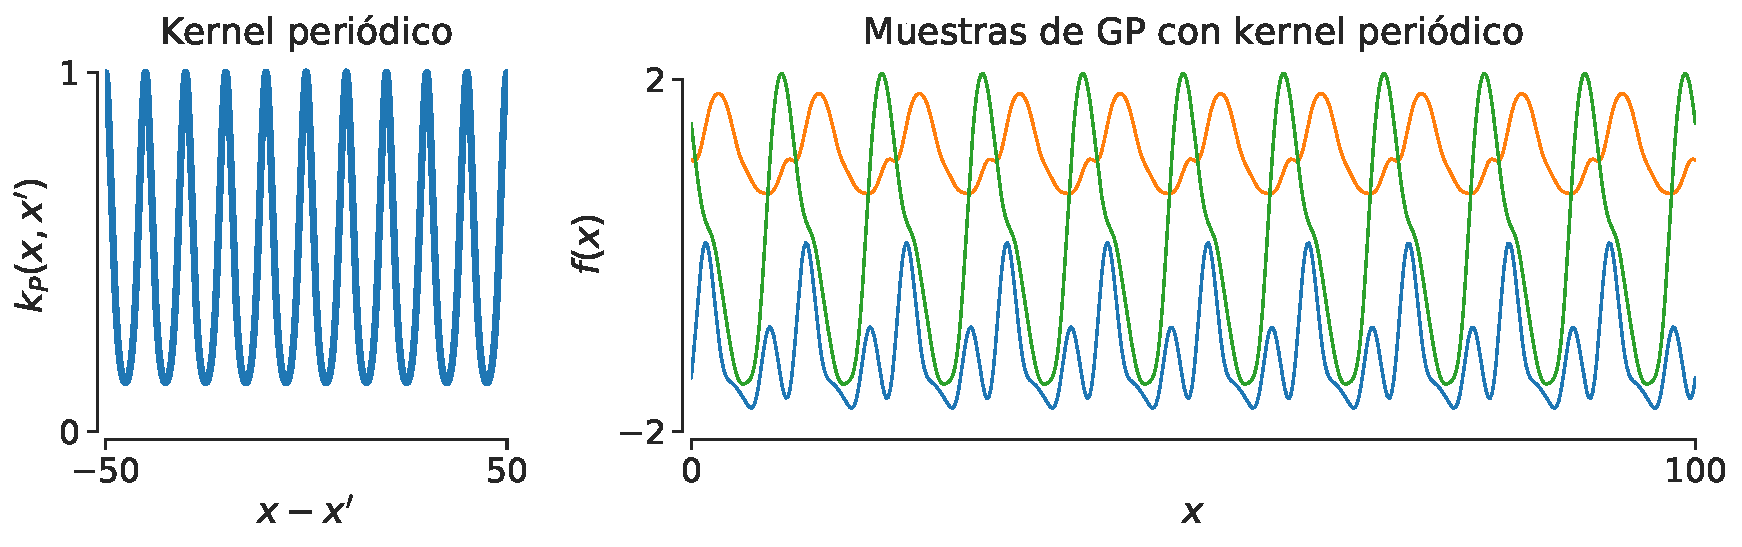
\includegraphics[width=0.9\textwidth]{img/cap8_muestras_P.pdf}
	\caption{Kernel periódico, en la izquierda se muestra la covarianza en función de su argumento $\tau=x-x'$, a la derecha de un $\gp$ usando un kernel periódico.}
	\label{fig:gp_7}
\end{figure}

\subsubsection{Operaciones con kernels}
A la hora de diseñar un $\gp$ y elegir una función de covarianza, no se está completamente limitado a kernels conocidos, sino que también se pueden combinar para obtener distintas funciones de covarianza y representar mejor el proceso.

Tanto la suma y multiplicación de kernels da como resultado un kernel válido que puede ser utilizado, también la exponencial de un kernel es también es un kernel, es decir $\exp(k_1(\cdot, \cdot))$ con $k_1$ un kernel válido.

\subsubsection{Representación espectral}
Un teorema importante para las funciones de covarianza en procesos débilmente estaicionarios es el teorema de Wiener–Khinchin, el cual dice que si para un proceso débilmente estacionario existe una función de covarianza $k(\tau)$ finita y definida para cualquier $\tau=x-x'$, entonces existe una función $S(\xi)$ tal que:

\begin{equation}\label{eq:gp_spectral}
	k(\tau) = \int S(\xi)e^{2\pi i \xi \cdot \tau} d\xi, \quad S(\xi)=\int k(\tau)e^{-2\pi i \xi \cdot \tau} d\tau
\end{equation}

Donde $i$ es la unidad imaginaria. $S(\xi)$ es conocida como la densidad espectral de potencia (PSD), en otras palabras, la función de covarianza $k(\tau)$ y la PSD $S(\xi)$ son duales de Fourier el uno del otro. Esto es extremadamente útil a la hora de diseñar funciones de covarianza pues este puede ser llevado a cavo en el dominio de la frecuencia y luego llevado a una función de covarianza usando la transformada inversa de Fourier.

\subsection{Extensiones para un \texorpdfstring{$\gp$}{GP}}
A continuación veremos un número de extensiones que se le pueden hacer a un $\gp$ para abordar distintos tipos de problemas.

\subsubsection{\texorpdfstring{$\gp$}{GP}de clasificación}

\begin{wrapfigure}{r}{0.35\textwidth}
\centering
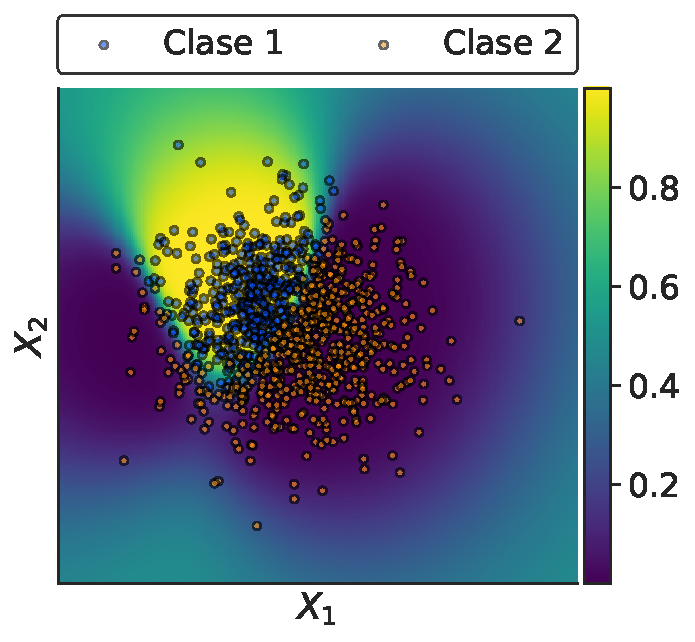
\includegraphics[width=0.3\textwidth]{img/cap8_classificacion}
\caption{$\gp$ de clasificación utilizando datos sintéticos. Este clasificador entrega una densidad de probabilidad en vez de una sola función de decisión.}\label{fig:gp_8}
\end{wrapfigure} 

Hasta el momento hemos visto como usar un $\gp$ para regresión, pero este también puede usado para clasificación, para esto simplemente ``pasamos'' nuestro $\gp$ por una función logística, para así obtener un prior sobre $\sigma\left(f(x)\right)$ donde $\sigma$ es la función logística. Sin embargo esto trae consigo un problema, pues ahora la distribución posterior a las observaciones no se tiene de forma analítica como para el caso de regresión, esto lleva a que tengamos que recurrir a métodos aproximado de inferencia. Una solución simple es utilizar la aproximación de Laplace, pero si se quieren aproximaciones más fidedignas métodos más complejos pueden ser usados como \textit{Expectation Maximization} y métodos MCMC. En la Fig.\ref{fig:gp_8} se muestra un ejemplo con datos sintéticos, a diferencia de la mayoría de los clasificadores vistos, este entrega naturalmente una densidad de probabilidad para la función de decisión.\\

\subsubsection{Selección automática de relevancia (ARD) (\textit{Selección automática de features})}
Un $\gp$ define una densidad de probabilidad sobre funciones, donde estas funciones son del tipo $f: \mathbb{R}^D \rightarrow \mathbb{R}$, con $D$ es finito, este es nuestra dimensión de entrada o ``características''. Haciendo un pequeño cambio en nuestra función kernel podemos hacer que esta automáticamente seleccione las entradas más relevantes con el problema, es decir realice una selección de características automática.\\

Si tomamos el kernel de la Ec.(\ref{eq:gp_ard}) vemos que es una multiplicación de kernels SE, donde se tiene un \textit{lenghtscale} por cada entrada $\ell_d$, sabemos que mientras más grande es este $\ell_d$ menos flexible será el $\gp$ respecto a cambios en ese eje, haciendo que las funciones del proceso dependan cada vez menos de la componente $d$ a medida que $\ell_d \rightarrow \infty$. De esta forma se puede controlar de forma automática la relevancia de cada eje del conjunto de entrada, pues los parámetros del kernel se obtienen en el entrenamiento. De esta forma estamos optimizando también en que grado afecta cada variable en nuestra predicción.

\begin{equation}\label{eq:gp_ard}
	k(x, x') = \sigma^2 \exp\left( -\sum_{d=1}^{D} \frac{(x_d - x_d')^2}{2\ell_d^2}\right)
\end{equation}


\subsubsection{Multi output \texorpdfstring{$\gp$}{GP}}
Hasta el momento solo hemos hablado de $\gp$ cuando nuestro proceso es solo una dimensión de salida. Se pueden extender los procesos Gaussianos a funciones de más de una salida o canal, donde ahora la función de covarianza $k(x, x')$ no entrega un escalar sino una matriz definida positiva, donde la diagonal corresponde a la covarianza del canal o autocovarianza y los elementos fuera de la diagonal corresponden a las covarianzas cruzadas o cross-covarianza. Este tipo de procesos Gaussianos aumentan considerablemente de complejidad al diseñar funciones de covarianza.\\ 

Dado un número $m$ de canales, se tendrán $m$ funciones de autocovarianza y ahora $m(m-1)/2$ funciones de covarianza y $k(x, x')$ será una matriz de $m\times m$. El desafio está en diseñar o escoger estas funciones de tal forma que para cualquier par de puntos $x$, $x'$ la matriz $k(x, x')$ sea definida positiva.

Una opción simple es asumir que los canales son independientes entre sí, lo que equivale a entrenar independientemente $m$ procesos Gaussianos, uno para cada canal, esto facilita el diseño de las funciones de covarianza pero hace que se pierdan relaciones entre los canales.
 

\subsection{Diferentes interpretaciones de un \texorpdfstring{$\gp$}{GP}}

\subsubsection{De regresión lineal a \texorpdfstring{$\gp$}{GP}}

Partiendo de la regresión lineal donde el modelo es:

\begin{equation}
	y_i = w X_i + \epsilon_i
\end{equation}

Donde $\epsilon_i \sim \mathcal{N}(0, \sigma_n^2)$, luego podíamos extender este modelo usando $M$ funciones base $\phi_m$ y obtener:

\begin{equation}
	y_i = \sum_{m=1}^{M} w_m \phi(x_i) + \epsilon_i
\end{equation}

El paso siguiente es la regresión Bayesiana en base de funciones, donde agregamos un prior sobre los pesos $w_m \sim \mathcal{N}(0, \lambda_m^2)$, donde si obtenemos la covarianza de este proceso y marginalizamos por los pesos $w_m$ obtenemos:

\begin{equation}
	Cov(x, x') = k(x, x') = \sum_{m=1}^{M} \lambda_m^2 \phi_m(x)^T\phi_m(x') + \delta_{x, x'} \sigma_n^2
\end{equation}

Donde $\delta_{x, x'}$ el delta de Kronecker. Si nos damos cuenta esto define un $\gp$ con la función covarianza con un número finito de funciones bases. En general los $\gp$ corresponderán a covarianzas con infinitas funciones bases, como veremos a continuación.\\

Tomando un modelo sin ruido, con un número $M$ de funciones base $\phi_m$, donde sobre los pesos se define un prior i.i.d $w_m \sim \mathcal{N}(0, \sigma^2)$, tenemos:

\begin{equation}
	f(x) =  \sum_{m=1}^{M} w_m \phi(x)
\end{equation}
Y tomando $\phi=\exp(-\frac{1}{2\ell^2}(x- c_i)^2)$ donde $c_i$ son los centros de estas bases, y luego haciendo tender el número de funciones base $M$ a infinito tenemos que la covarianza es:

\begin{align}
	\mathbb{E}\left\{f(x) f(x')\right\} & = \sigma^2\sum_{m=1}^{M}  \phi_m(x)\phi_m(x') && \text{tomando } M\rightarrow \infty\\
	\mathbb{E}\left\{f(x) f(x')\right\} & \rightarrow \sigma^2 \int e^{-\frac{1}{2\ell^2}(x- c)^2} e^{-\frac{1}{2\ell^2}(x'- c)^2} dc \\
	& = \sigma^2 \sqrt{\pi\ell^2} e^{-\frac{1}{4\ell^2}(x- x')^2}\\
	& = k_{SE}(x, x')
\end{align}

Donde vemos que efectivamente el kernel SE es una función de covarianza para una composición infinita de funciones base.

\subsubsection{Nota sobre RKHS}
Dado un conjunto de entrenamiento $(X, Y) = \{x_i, y_i \}_{i=1}^{n}$ condicionando el proceso solo a una muestra de test $X_*=x_*$ y asumiendo una función media nula, de la Ec.(\ref{eq:gp_post}) para un $\gp$ la posterior de la media está dada por:

\begin{equation}
	\bar{f}(x_*) = m_{x_*|X} = k(X, x_*) (k(X, X) + \sigma_n \eye)^{-1} Y
\end{equation}

Y tomamos el vector $\bm{\alpha} = \left(k(X, X) + \sigma_n \eye \right)^{-1} Y$ obtenemos la expresión:

\begin{equation}
	\bar{f}(x_*) = \sum_{i=1}^{n} \alpha_i k(x_i, x_*)
\end{equation}

Donde, a pesar de que el proceso esta descrito por (posiblemente infinita) funciones base, aún así es la suma de finitos términos, cada uno centrado en un punto de entrenamiento, esto es debido al teorema del representante de los Espacios de Hilbert de Kernel Reproductor (RKHS). La intuición detrás de esto es que incluso si el $\gp$ induce una distribución conjunta sobre todos los $y = f(x)$, una para cada $x$ en el dominio, al hacer predicciones en el punto $x_*$ solo nos interesa la distribución $(n+1)$-dimensional definida por los puntos de entrenamiento más este punto de test.

%!TEX root = ../notas_de_clase.tex

\section{Aprendizaje no supervisado}

\subsection{Reducción de dimensionalidad}

El problema de reducción de dimensionalidad consiste con construir una representación de dimensión estrictamente menor que los datos originales con la finalidad de interpretar de mejor forma la información contenida en nuestros datos así como también disminuir el costo computacional en el entrenamiento.

\subsubsection{Maldición de la dimensionalidad}

La maldición de la dimensionalidad o efecto Hughes es un conjunto de fenómenos que ocurren al realizar análisis sobre datos de alta dimensión, los cuales en algunos casos tienden a aumentar el costo computacional de forma exponencial en la dimensión.

\subsubsection{Análisis de componentes principales (PCA)}

Consideremos ahora un conjunto de observaciones de $\{\x_i\}_{i=1}^N\subset\R^M$, donde denotamos $\x_i=[x_{i1},x_{i2},\ldots,x_{iM}]^\top$. Podemos entender que el elemento $x_{ij}$ corresponde al valor del atributo $j$ para la observación $i$. 

Notemos que cada observación puede descomponerse en la base canónica $\{\e_i\}_{i=1}^M$ de $\R^M$ de la forma 
\begin{equation}
	\x_i = x_{i1}\e_1 +  x_{i2}\e_2 + \cdots + x_{iM}\e_M 		
\end{equation}
Notemos que es posible representar cada vector $\x_i$ mediante una cantidad $M'<M$ de términos, truncando la representación anterior, es decir,  
\begin{equation}
	\x_i \approx \sum_{j=1}^{M'} x_{i\sigma(j)}\e_{\sigma(j)}
\end{equation}
donde $\sigma:\{1,2,\ldots,M\}\mapsto\{1,2,\ldots,M\}$ es una permutación que prioriza las coordenadas más representativas de los datos. Dichas aproximaciones de las observaciones $\{\x_i\}_{i=1}^N$ son una versión de baja dimensión, entonces, naturalmente nos podemos hacer la siguiente pregunta: dado una dimensión $M'<M$  ¿es efectivamente un subconjunto de los vectores canónicos la mejor base para descomponer las observaciones?  ¿cómo encontramos la \emph{mejor} base?

\begin{figure}[H]
	\centering
	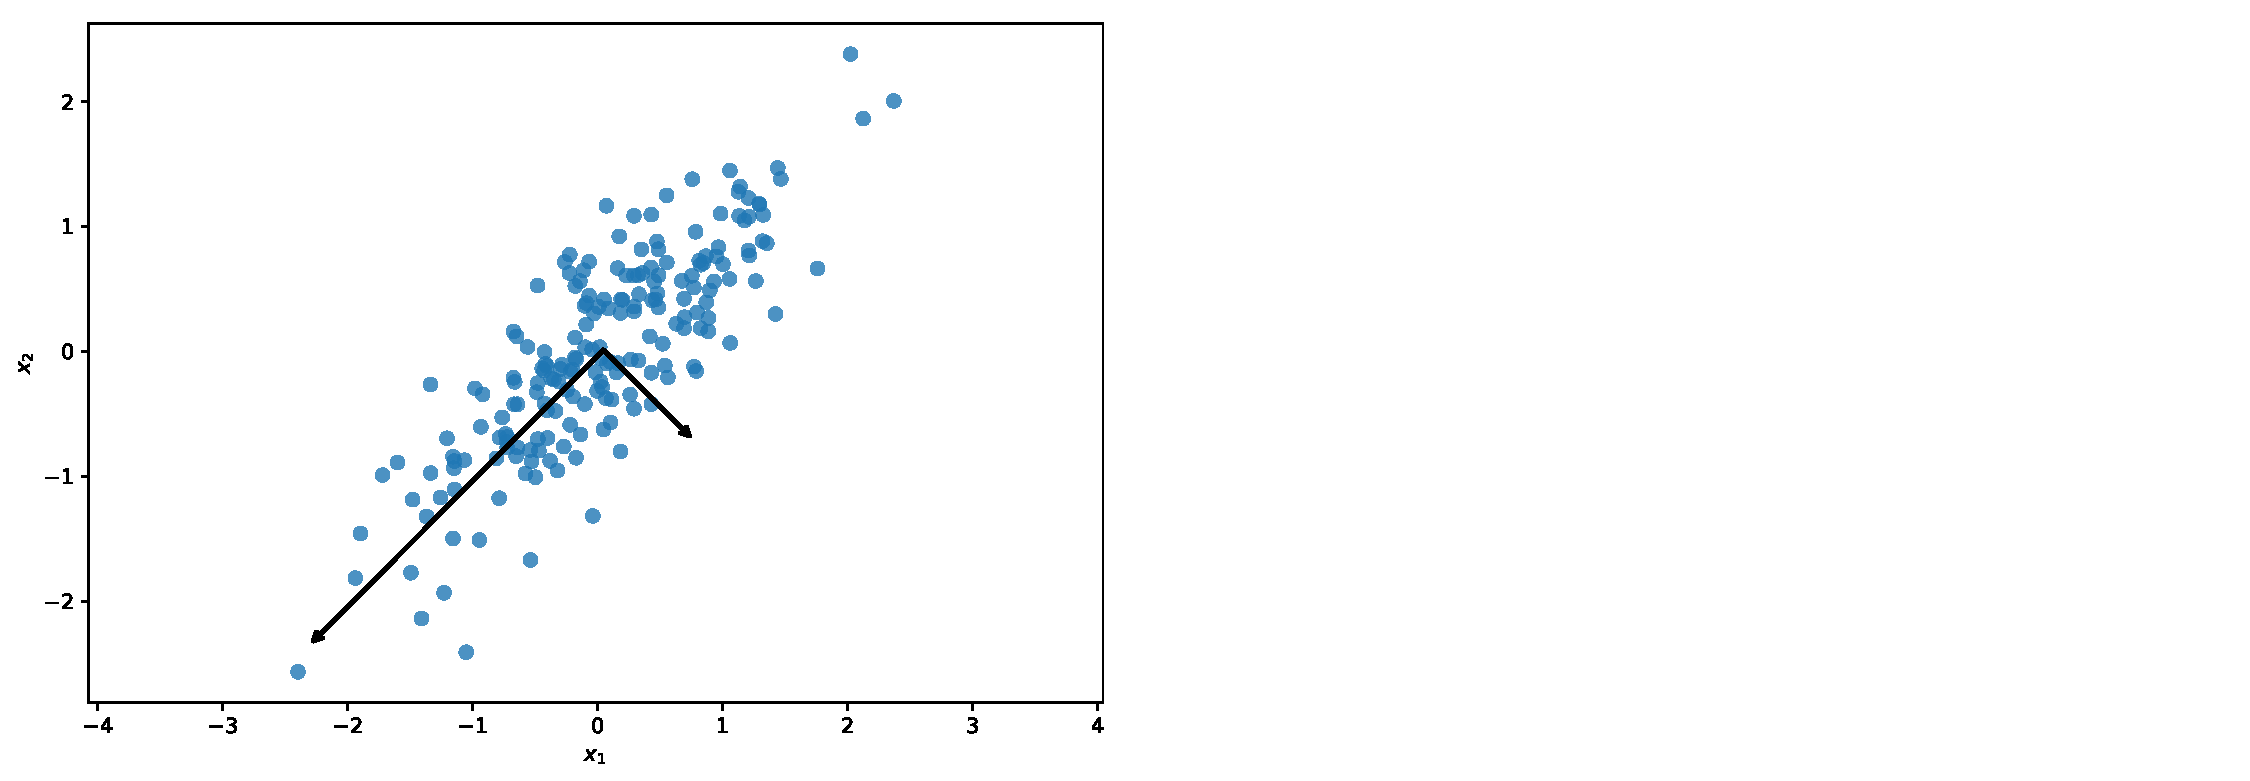
\includegraphics[width=0.6\textwidth]{img/cap8_pca.pdf}
	\caption{Base ortogonal de $\R^2$ formada por las componentes principales de los datos. Se observa en este caso que ninguna de las componentes principales corresponde a un vector de la base canónica. El eje que cruza los cuadrantes 1 y 3 corresponde a $\cvector_1$ y el otro, a $\cvector_2$.}
	\label{fig:ej_fda}
\end{figure}

La respuesta a la primera pregunta es, en la mayoría de los casos, negativa. Esto es porque los elementos de la base canónica, por sí solos, conllevan poca información estructural que puede ser encontrada en los vectores observados. En particular, consideremos el caso en donde solo se dispone de dos observaciones $\{\x_1, \x_2\}$, si $M'=2$, entonces una descomposición que garantiza error nulo es simplemente elegir $\x_1$ y $\x_2$ como bases de la nueva descomposición, donde los coeficientes estarían dados por $[1,\ 0]^\top$ y $[0,\ 1]^\top$.\\

Para encontrar la \emph{mejor} base, lo primero que se requiere es definir qué se entiende por \emph{mejor}. Nos enfocaremos en determinar una base cuyos componentes \textbf{ordenados} $\cvector_1,\cvector_2,\ldots$ capturan las $M'$ direcciones ortogonales de máxima variabilidad de nuestros datos. De esta forma, dado que $\langle\cvector,\x\rangle$ representa la proyección ortogonal de $\x$ sobre $\cvector$, el primer elemento de la nueva base estará dado por 
\begin{equation}
	\cvector_1 = \argmax_{||\cvector||=1} {\langle\cvector,\x\rangle} \label{eq:PCA_max}
\end{equation}
Este criterio es conocido como \textbf{análisis de componentes principales (PCA)}. Notemos que la restricción $||\cvector_1||=1$ es necesaria ya que $\langle\lambda\cvector_1,\x\rangle = \lambda\langle\cvector_1,\x\rangle$ por lo que $\langle\cvector_1,\x\rangle$ puede crecer indefinidamente si no se fija una restricción sobre la norma de $\cvector$. Por esta razón, s.p.g. podemos fijar la norma de $\cvector_1$ en 1 y buscar una base ortonormal. Además, es importante estandarizar los datos:

\begin{itemize}
	\item Características de media nula: la matriz $X$ con $(X)_{ij} = (\x_i)_j$ debe tener columnas con media $0$. Esto se consigue restando la media de la columna a cada una de las entradas de dicha columna. El objetivo de este ajuste es poder centrar los datos.
	\item Varianzas marginales unitarias: si una dimensión tiene una varianza marginal mayor que el resto, ésta será más importante en la determinación de la dirección de máxima varianza solo por su magnitud y no por la relación entre variables. La normalización se consigue dividiendo cada entrada de la columna por la desviación estándar de la columna.
\end{itemize}

Como en general no contamos con la distribución de las observaciones $p(\x)$, podemos considerar una aproximación muestral de la varianza en la ecuación \eqref{eq:PCA_max} y resolver 
\begin{align}
	\cvector_1 = \argmax_{||\cvector||=1} \sum_{i=1}^N \langle\cvector,\x_i\rangle^2.\label{eq:PCA_max2}
\end{align}

Podemos ahora usar la siguiente notación
$$
X=\begin{bmatrix}
        \x_1^\top\\
        \vdots\\
        \x_N^\top\\
        \end{bmatrix}=
        \begin{bmatrix}
        {x}_{11}    & \dots & {x}_{1M}  \\
        \vdots          & \ddots& \vdots        \\
        {x}_{N1}    & \dots & {x}_{NM}
        \end{bmatrix}
$$
y reescribir la ecuación \eqref{eq:PCA_max2} como 
\begin{equation}
	\cvector_1 = \argmax_{||\cvector||=1} ||X\cvector||^2 
			= \argmax_{||\cvector||=1} \cvector^\top X^\top X \cvector
			= \argmax_{\cvector} \frac{\cvector^\top X^\top X \cvector}{\cvector^\top \cvector}
			\label{eq:PCA_max3}
\end{equation}

Por otra parte, se tiene la siguiente propiedad:

\begin{lemma}[minimización del cociente de Rayleigh]

Sea $M\in\mathcal{M}_{nn}(\R)$ matriz cuadrada simétrica, entonces, para el cociente de Rayleigh

\begin{equation}
	R(M,x):=\frac{x^\top Mx}{x^\top x}
\end{equation}

Su valor mínimo corresponde al menor valor propio de $M$, y es alcanzado en su vector propio asociado.

\end{lemma}

\begin{proof}
	Dado que $R(M,cx)=R(M,x)$ para todo $c\neq 0$, basta verlo para $\norm{x}=1$, por lo que se puede considerar como una restricción adicional. Por teorema de Lagrange:
	
	\begin{equation}
		L(x,\lambda) = x^\top Mx - \lambda(\norm{x} - 1)\implies \frac{\partial L}{\partial x} = 2x^\top M - 2\lambda x^\top = 0 \implies Mx=\lambda x
	\end{equation}
	
	Por lo tanto, los puntos críticos de lagrangiano son los vectores propios $v_i$ de $M$. Por otra parte:
	
	\begin{equation}
		R(M,v_i)=\frac{v_i^\top Mv_i}{v_i^\top v_i} = \frac{v_i^\top \lambda_i v_i}{v_i^\top v_i} = \lambda_i\in\R \text{ ya que $M$ es simétrica.}
	\end{equation}
	
Por lo tanto, el valor mínimo de $R(M,x)$ es $\lambda_{min}$ y es alcanzado en el vector propio asociado $v_{min}$. Por el mismo argumento, el valor máximo es $\lambda_{max}$ y es alcanzado en $v_{max}$.
\end{proof}

De esta forma, dado que $X^\top X$ es simétrica, su cociente de Rayleigh es maximizado en el vector propio asociado al valor propio máximo de $X^\top X$. Consecuentemente, la proyección de una observación $\x_i$ en la dirección de máxima varianza, o bien la \emph{primera componente principal}, está dada por 
\begin{equation}
	\x_i^{(1)} = \langle \x_i, \cvector_1 \rangle
\end{equation}
donde $\cvector_1$ es el vector propio asociado al mayor valor propio de la matriz de covarianza muestral $XX^\top$.\\

El cálculo de las siguientes componentes se realiza de forma iterativa sobre los residuos del conjunto de observaciones con respecto a las componentes anteriores. De esta forma, PCA encuentra una nueva base ortonormal tal que las componentes maximicen la variabilidad donde en algunos casos se puede perder intepretabilidad de las nuevas características generadas, pues son combinaciones lineales de las características originales de los datos. A pesar de esto, utilizando las primeras 2 o 3 componentes PCA se pueden visualizar datos de alta dimensionabilidad de forma ilustrativa.


\subsubsection{Kernel PCA}
El método Kernel PCA es similar a PCA, pero esta vez se utiliza el truco del kernel para proyectar los datos. En ese sentido, en vez de calcular la matriz de covarianza empírica $X^\top X$, se utiliza la matriz de Gram dada por un kernel $K$ donde

$$
K_{ij} = K(x_i,x_j) = \langle\phi(x_i),\phi(x_j)\rangle
$$

Luego, se realiza PCA utilizando dicha matriz.\\

En la Figura \ref{fig:kpca} se puede observar un ejemplo en que el resultado de linear PCA no es suficiente, puesto que el problema es simétrico, mientras que KPCA realiza una correcta separación de ambos clusters.

\begin{figure}[ht]
    \centering
    \includegraphics[width=0.7\linewidth]{img/cap7_kpca.pdf}
    \caption{Ejemplo de KPCA sobre un conjunto de datos que no es linealmente separable.}
    \label{fig:kpca}
\end{figure}

\subsubsection{Probabilistic PCA}
PCA probabilístico (PPCA) tiene su inspiración en que PCA se puede expresar como la solución vía máxima verosimilitud de un modelo probabilístico de variable latente. De este modo, PPCA propone un método iterativo para obtener la solución evaluando solo cierto número de componentes, sin necesidad de calcular la matriz de covarianza empírica.

El modelo probabilístico para PCA en el que se inspira PPCA es el siguiente:\\

Sean $(x_i)_{i=1}^N\subset \mathbb{R}^M$ los elementos observados, inputs o variables y $z\in \mathbb{R}^l$ una variable latente explícita correspondiente al espacio de las componentes principales. Bajo la hipótesis de un modelo de observación lineal:

\begin{equation}
	x=Wz+\mu+\epsilon
\end{equation}

Donde $\epsilon\sim\mathcal{N}(0,\sigma^2)$ es un sumando de ruido y $W\in \R^{M\times l}$, $\mu \in \R^M$ y $\sigma^2$ son parámetros a determinar, se define el siguiente prior para $z$:

\begin{equation}
p(z) = \mathcal{N}(0,\eye)
\end{equation}

De este modo, la distribución condicional de x dado z también es gaussiana:

\begin{equation}
p(x|z) = \mathcal{N}(Wz+\mu,\sigma^2\eye)
\end{equation}

Notemos que no se pierde generalidad tomar el prior para $z$ con media cero y varianza unitaria, puesto que si se toma otro prior más general, se produce el mismo modelo.\\


Dado que tenemos un modelo paramétrico probabilístico, podemos estimar los parámetros con máxima verosimilitud. Dado los datos $\mathcal{D} = \{x_i\}_{i=1}^N$, la log-verosimilitud está dada por:

\begin{align}
\log p(\mathcal{D}|W,\mu, \sigma^2) & = \sum_{i=1}^N \log p(x_i|W,\mu, \sigma^2)\\
& = \frac{NM}{2}\log (2\pi) - \frac{N}{2}log|C| - \frac{1}{2}\sum_{i=1}^N (x_i-\mu)^T C^{-1} (x_i-\mu),
\end{align}

con $C = WW^T + \sigma^2 I$.

Usando la condición de primer orden obtenemos

\begin{equation}
	\mu = \bar{x} = \frac{1}{N}\sum_{i=1}^N x_i
\end{equation}

De esta manera tenemos la función de log-verosimilitud completa:

\begin{align}
    \log p(X, Z|W, \mu, \sigma^2) = \sum_{i=1}^N \{\log p(x_i|z_i) + \log p(z_i)\}
\end{align}

y evaluando en $\mu = \bar{x}$

\begin{align}
\notag \mathbb{E}[ p(X,Z |W, \mu, \sigma^2) ] =  -\sum_{i=1}^N \Bigg\{ &\frac{l}{2} \log (2\pi \sigma^2)\\
\notag & + \frac{1}{2}\text{Tr}(\mathbb{E}[z_iz_i^T])\\
\notag & \frac{1}{2\sigma^2}||x_i - \mu||^2 - \frac{1}{\sigma^2}\mathbb{E}[z_i]^T W^T (x_i - \mu)\\
& \frac{1}{2\sigma^2} \text{Tr}(\mathbb{E}[z_iz_i^T]W^T W) \Bigg\}
\end{align}

\subsubsection{Discriminante lineal de Fisher}

Para evitar los artefactos (sesgos) introducidos por clases  asimétricas en el uso de mínimos cuadrados para clasificación, es posible interpretar el problema de clasificación como uno de \emph{reducción de dimensionalidad}, en donde la reducción consiste representar nuestros datos  en solo una dimensión, la cual representa su (grado de pertenencia a una) clase. Con este objetivo en mente, consideremos el problema de clasificación binaria de $x\in \R^M$, donde proyectamos $x$ en un espacio \textbf{unidimensional} con respecto a un vector $a\in\R^M$ de acuerdo a:

\begin{equation}
	y = a^\top x,
\end{equation}

donde podemos definir un umbral $b$ para asignar $x$ a $\cC_1$ si $y+b\geq 0$ y $x$ a $\cC_2$ en caso contrario. Notemos que de esta forma recuperamos el modelo lineal para clasificación.\\

En general, al proyectar un objeto $M$-dimensional en un espacio  1-dimensional, se pierde gran parte de la información, lo cual genera el hecho de que clases claramente separadas en el espacio $M$-dimensional puedan traslaparse al ser proyectadas a 1 dimensión cuando la elección del vector $a\in\R^M$ no es la mejor. Sin embargo, es posible ajustar el vector $a$ con la finalidad de obtener una proyección de $x$ que maximice el grado de separación entre clases.\\

Con el objetivo de encontrar el vector $a$ que cumple con este requerimiento en base a un conjunto de datos  $\datos$, primero definamos las cardinalidades de clases mediante $N_1 = |\{x\in\datos:x\in\cC_1\}|$ y $N_2 = |\{x\in\datos:x\in\cC_2\}|$, lo cual permite calcular los promedios muestrales (centros de masa) de cada  clase mediante: 
\begin{equation}
	\mu_1=\frac{1}{N_1}\sum_{n\in\mathcal{C}_1}x_n,
	\quad\quad\quad
	\mu_2=\frac{1}{N_2}\sum_{n\in\mathcal{C}_2}x_n.
\end{equation}
La medida más simple de separación entre las proyecciones de las clases sobre $a$ es la distancia entre las medias  de sus proyecciones:
\begin{equation}
	m_1 - m_2 = a^\top(\mu_1-\mu_2),
\end{equation}
donde $m_k= a^\top\mu_k$ corresponde al promedio de los elementos de  la clase $\mathcal{C}_k$ proyectado sobre el  vector $a$ (centro de masa sobre la recta). Consecuentemente, el vector $a$ que maximiza la distancia entre la proyección de clases es el que maximiza la expresión anterior. Sin embargo, esta expresión puede ser arbitrariamente grande si escalamos $a$, por lo que se fijará $\left \| a \right \|_2=1$. Además, por la desigualdad de Cauchy-Schwarz, $|a^\top(\mu_1-\mu_2)|\leq \norm{a}\norm{\mu_1-\mu_2}$ con igualdad si y solo si los vectores son paralelos. De este modo, se llega a que $a\propto(\mu_1-\mu_2)$. \\

Una desventaja de este enfoque, en el cual se ha ignorado la dispersión de las clases y solo se ha considerado su media, es que pueden existir 2 clases bien separadas en el espacio $D$-dimensional, pero que al proyectar los datos sobre la recta que une sus promedios, las proyecciones de cada clase se traslapen. 

\begin{figure}[H]
	\centering
	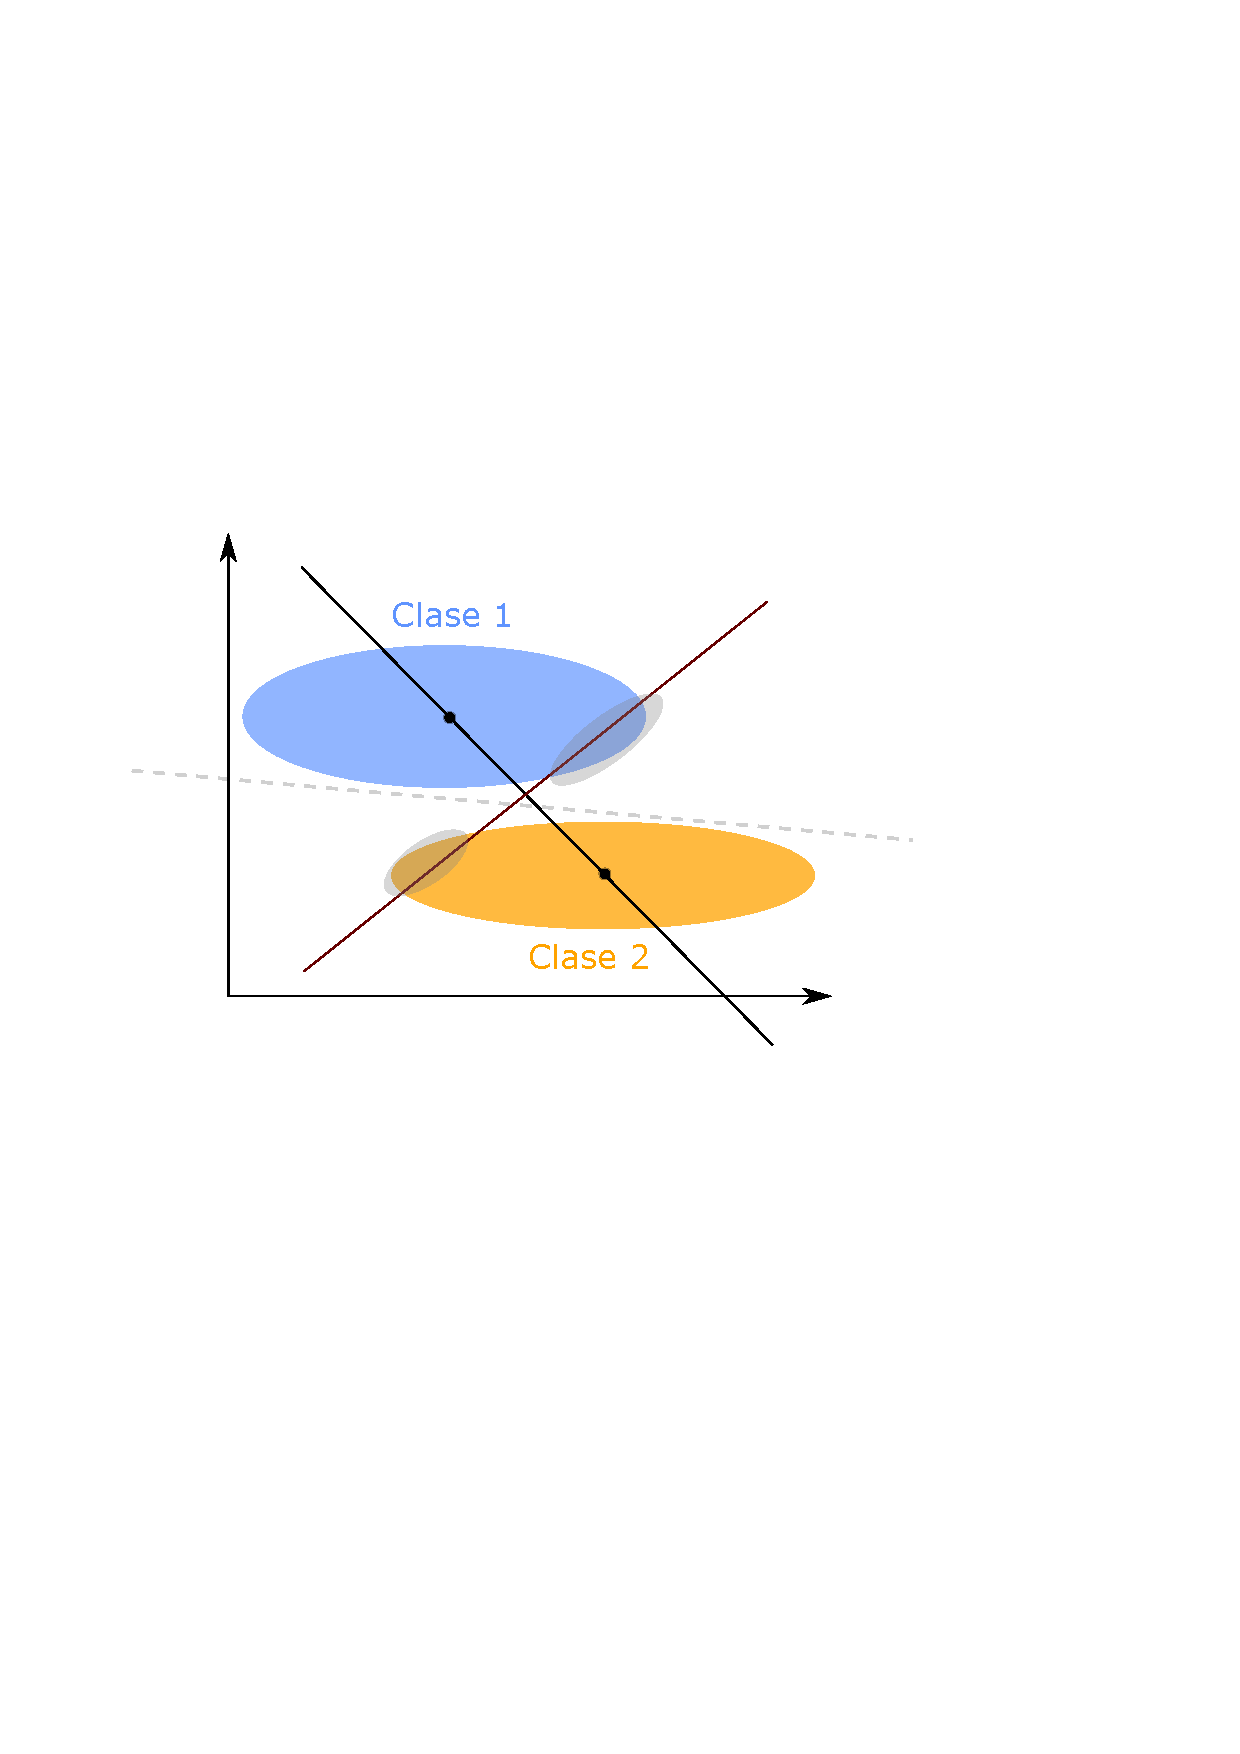
\includegraphics[width=0.6\textwidth]{img/cap6_fisher.pdf}
	\caption{Superposición de las proyecciones al considerar únicamente la recta que une las medias de clase. La recta roja determina la región de decisión y la recta segmentada muestra un posible hiperplano separador.}
	\label{fig:ej_fda}
\end{figure}

Para resolver este problema, Fisher propuso maximizar no solo distancia entre las (medias de las) clases proyectadas, sino que adicionalmente minimizar la dispersión de los elementos de una misma clase, con el objetivo de disminuir el traslape entre las proyecciones de las clases. Como medida de dispersión, definimos la varianza muestral proyectada de los elementos de la clase $\cC_k$ mediante
\begin{align}
	s_k^2 &= \sum_{n\in \mathcal{C}_k}(a^\top(x_n-\mu_k))^2\\
	&= \sum_{n\in \mathcal{C}_k}(y_n-m_k)^2,
\end{align}
Donde el factor de correción $\frac{1}{N_k-1}$ fue omitido ya que de lo contrario, todas las clases pesarían lo mismo sin importar la cantidad de elementos de la clase. Lo anterior nos permite definir la siguiente función objetivo
\begin{equation}
J(a) = \frac{m_1-m_2}{s_1^2+s_2 ^2},
\end{equation}
donde explícitamente vemos la discrepancia ``inter'' clases en el numerador y la discrepancia  ``intra '' clases en el denominador. Adicionalmente, podemos expresar este costo directamente como función del vector de proyección $a$:
\begin{equation}
	J(a) = \frac{a^\top S_B a}{a^\top S_Wa},
\end{equation}
donde la matriz de covarianza entre clases $S_B$ y matriz total de covarianza dentro de clases $S_W$ están respectivamente dadas por
\begin{align}
	S_B &= (\mu_1-\mu_2)(\mu_1-\mu_2)^\top\\
	S_W &= \sum_{n\in \cC_1}(x_n-\mu_1)(x_n-\mu_1)^\top +
	\sum_{n\in \cC_2}(x_n-\mu_2)(x_n-\mu_2)^\top. 
\end{align}
Aplicando la condición de primer orden para $J(a)$, obtenemos que el vector $a$ óptimo debe cumplir
\begin{equation}
	(a^\top S_B a)S_W a = (a^\top S_W a)S_B a.	
\end{equation}
Sin embargo, notemos que la norma del vector  $a$ es irrelevante, solo interesa su orientación, con lo que  ignorando los escalares $(a^\top S_B a)$ y $(a^\top S_W a)$ tenemos que la relación de optimalidad es $S_W a \propto S_B a$. Además, por la definición de $S_B$, sabemos que $S_B a\propto(\mu_1-\mu_2)$, con lo que la relación de optimalidad se convierte en es $S_W a \propto (\mu_1-\mu_2)$. Consecuentemente, el vector optimo $a$ en el  criterio de Fisher debe cumplir
\begin{equation}
	a \propto S_W^{-1}(\mu_1-\mu_2).
\end{equation}

La Figura \ref{fig:ej_fda} muestra el  discriminador lineal que solo considera los promedios a la  izquierda y la corrección de Fisher a la derecha. Observemos cómo el incluir una medida de la dispersión de los datos es clave para lograr un mejor discriminador.

\begin{figure}[H]
	\centering
	\includegraphics[width=0.8\textwidth]{img/cap2_dos_clases_proyeccion.pdf}
	\caption{Discriminador lineal considerando solo la media entre clases (izquierda) y  su extensión mediante la corrección de Fisher que incorpora la varianza muestral de los datos.}
	\label{fig:ej_fda}
\end{figure}

\subsection{Clustering}

Otro de los problemas principales del aprendizaje no supervisado es poder agrupar las entradas sin necesidad de que estas tengan etiquetas (como ocurre en los métodos de clasificación). La dificultad principal de esta tarea es que es necesario definir un concepto de similitud entre las distintas entradas para poder particionar los datos en grupos (clusters) de características similares.

\subsubsection{Hierarchical clustering (HCA)}

Corresponde al algoritmo de clustering más simple pero a su vez, es uno de los más caros computacionalmente. El objetivo es identificar $k$ clusters en los datos.\\

 El algoritmo aglomerativo de clustering es el siguiente:

\begin{enumerate}
	\item Para comenzar, se considerarán $n$ clusters distintos. Asignar a cada elemento un cluster único.
	\item Buscar el par de clusters más similar (bajo algún criterio) y combinarlos en un solo cluster.
	\item Repetir el paso anterior hasta tener $k$ clusters.
\end{enumerate}

Para dos clusters $A,B\subset\mathcal{D}$, los criterios de similitud más frecuentes son los siguientes:

\begin{itemize}
	\item \textbf{Single-linkage clustering:} $D_s(A,B):=\min\{d(a,b):a\in A, b\in B\}$.
	\item \textbf{Complete-linkage clustering:} $D_s(A,B):=\max\{d(a,b):a\in A, b\in B\}$.
	\item \textbf{Average-linkage clustering:} $D_a(A,B):=\frac{1}{|A|\cdot|B|}\sum_{a\in A, b\in B} d(a,b)$.
\end{itemize}

Donde $d:\mathcal{D}\times \mathcal{D}\to \R_+$ es una métrica en $\mathcal{D}$. Elecciones distintas del criterio de similitud y/o métrica (generalmente euclidiana) pueden llevar a agrupaciones distintas.

\subsubsection{k-means}
Dado un entero $k \in \mathbb{N}$ y uin conjunto de observaciones $X = \{x_i\}_{i=1}$ con $x_i\in \mathbb{R}^D$ queremos separar los datos en k grupos, donde cada grupo se le asigna un centroide $\mu_k$ y cada elemento $x_i$ se le asigna el grupo que tenga el centroide más cercano.

Sea $r_{ik}$ la asignación, esta estará definida por:

\begin{align}
r_{ik} = \begin{cases}
1 & \text{si } k = \text{argmin}||x_i-\mu_k||\\
0 & \text{si no.}
\end{cases}
\end{align}
Es decir, para encontrar los centroides se debe minimizar la función:

\begin{align}
J = \sum_{i=1}^N \sum_{k=1}^K r_{ik} ||x_i-\mu_k||^2
\end{align}

Para minimizar esta función utilizaremos un enfoque llamado \emph{Expectation-Maximization}. Este es un método iterativo y como tal, tiene problemas con mínimo locales, pero para solucionar esto, basta inicializar el algoritmo muchas veces.\\

El algoritmo más frecuente usado para k-means es el algoritmo de Loyd:

\begin{itemize}
    \item \textbf{E-step:} En este paso, se calculan (actualizan) las asignaciones $r_{ik}$, dejando fijos $\mu_k$. Lo que corresponde a asignar el dato $x_i$ al centroide más cercano.
    \item \textbf{M-step:} El siguiente paso corresponde a actualizar los centroides $\mu_k$ dejando fijo las asignaciones $r_{ik}$.
    
    Como J es cuadrática en $\mu_k$, entonces podemos utilizar la condición de primer orden:
    \begin{align}
        \mu_k = \frac{\sum_{i=1}^N r_{ik}x_i}{\sum_{i=1}^N r_{ik}}
    \end{align}
    
    Lo que corresponde a asignar el centro del cluster al promedio de todas las muestras asignadas al antiguo cluster.\\
    
    El algoritmo termina cuando los centroides ya no cambian.
\end{itemize}


Para los centroides iniciales, se tienen dos posibles inicializaciones:

\begin{itemize}
	\item \textbf{Método de Forgy:} se eligen de forma aleatoria $k$ puntos de la muestra como centroides iniciales.
	\item \textbf{Random partition:} se eligen asignaciones aleatorias para los elementos. De este modo, los centroides iniciales serán los centroides obtenidos al realizar M-step.
\end{itemize}

El método de Forgy es preferido cuando se realiza k-means mediante el algoritmo de Lloyd.\\


\begin{figure}[h]
  \centering
  \includegraphics[width=0.7\textwidth]{img/cap7_k_medias}
  \caption{(Izquierda) Datos reales con sus etiquetas correctas. (Derecha) Clusters encontrados por k-means.}
  \label{fig:kmeans}
\end{figure}

\underline{\textbf{Ejemplo:}} En la figura \ref{fig:kmeans} se observa un ejemplo de clustering utilizando kmeans. Los clusters creados por kmeans son circulares, puesto que se utiliza distancia euclidiana hace el centro del cluster.\\


Por otra parte, la asignación de cluster mediante el centroide más cecano provoca que cada par de centroides divida al espacio ambiente en dos semiespacios mediante el hiperplano simetral que pasa entre ambos puntos. Luego, dado que la intersección finita de semiespacios genera un poliedro, se tiene que la partición generada por kmeans forma un diagrama de Voronoi.

\begin{figure}[h]
  \centering
  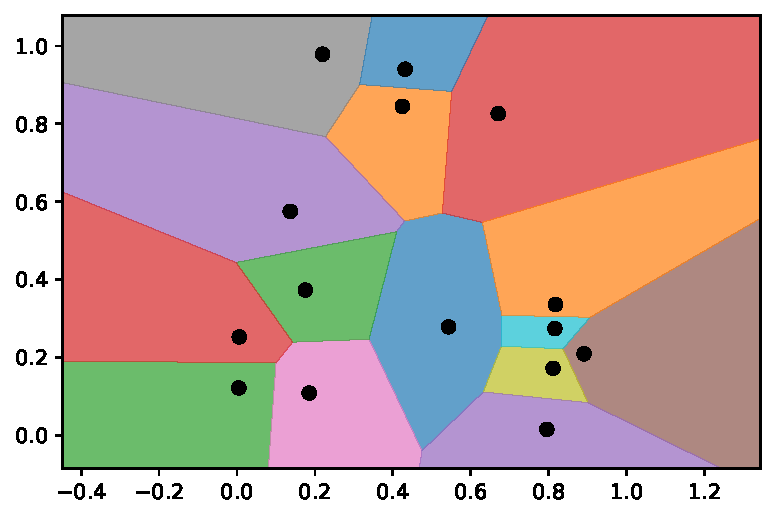
\includegraphics[width=0.6\textwidth]{img/cap8_voronoi}
  \caption{Partición de $\mathbb{R}^2$ inducida por los centroides.}
  \label{fig:kmeans}
\end{figure}


\subsubsection{Modelo de mezcla de gaussianas}

La mezcla de gaussianas (GMM) es un caso general de $k$-means, en donde los clusters pueden tener una forma anisotrópica modelada por una Gaussiana con covarianza no necesariamente proporcional a la identidad. Además, si bien su solución puede ser muy similar a K-means los supuestos subyacentes al modelo CMM son diferentes y obedecen a un enfoque de modelo generativo. \\


Una distribución de mezcla de gaussianas consiste en una combinación convexa de distribuciones gaussianas
\begin{equation}
	p(\x) = \sum_{k=1}^K \pi_k \mathcal{N}(\x| \mu_k,\Sigma_k)
\end{equation}

Donde una muestra $x$ es generada mediante dos etapas: primero se elige un cluster al azar y luego, se genera una muestra aleatoria dentro del cluster. Nos referiremos a los parámetros de este modelo como 

\begin{itemize}
	\item $\pi_k:$ coeficiente de mezcla del cluster  $k$ (probabilidad de venir del cluster $k$).
	\item $\mu_k:$ media del cluster  $k$.
	\item $\Sigma_k:$ matriz de covarianza del cluster  $k$.
\end{itemize}

Para ver que la formulación anterior es la indicada para la generación de $\x$, se puede asignar una variable latente $\z(\x) = \z = [z_1,z_2,\ldots,z_K]^\top\in\{0,1\}^K$, que describa la asignación de $\x$ a cada cluster, es decir, $z_{k}=1$ si la observación $\x$ pertenece al cluster $k$, y $z_{k}=0$ si no. Bajo esta notación, podemos denotar la distribución marginal del cluster $k$ (es decir, de que una observación sea generada por la $k$-ésima componente) como 
\begin{equation}
 	p(z_k=1) = \pi_k \label{eq:GMM_marg1}
\end{equation} 

Además, para una muestra $\x$ proveniente del cluster $k$ se tiene que

\begin{equation}
	p(\x|z_k=1) = \cN(\x|\mu_k,\Sigma_k)
\end{equation}

Por lo tanto, usando probabilidades totales:

\begin{equation}
	p(\x)=\sum_{k=1}^N p(z_k=1) p(\x|z_k=1) = \sum_{k=1}^N \pi_k \cN(\x|\mu_k,\Sigma_k)
\end{equation}

Lo cual prueba que el modelo sugerido al comienzo es el indicado para una mezcla de gaussianas.\\

Recordemos que los parámetros del modelo de mezcla de gaussianas son los coeficientes de mezcla, las medias y varianzas de cada componente. Si disponemos de un conjunto de observaciones $\{\x_i\}_{i=1}^N$, entonces podemos encontrar dichos parámetros mediante máxima verosimilitud. Observe que la log-verosimilitud está dada por 

\begin{equation}
	\log p(\x_1,\ldots,\x_N) = \sum_{n=1}^N \log p(\x_n) = \sum_{n=1}^N \log \sum_{k=1}^K  \pi_k\cN(\x_n|\mu_k,\Sigma_k) \label{eq:GMM_like}	
\end{equation}
Hay una serie de complicaciones relacionados a la búsqueda de estos parámetros mediante la maximización de las ecuación \eqref{eq:GMM_like}. Primero, están las soluciones dadas por singularidades cuando una muestra es exactamente igual a una de las medias, en cuyo caso un término de la log-verosimilitud es proporcional a $1/\sigma_k$, con lo que la maximización de $\sigma_k$ resulta en una log-verosimilitud infinita. En segundo lugar tenemos las redundancias de soluciones: para cada máximo local (o solución en general) de la log-verosimilitd existen $K!$ soluciones equivalente con la misma verosimilitud dadas por las permutaciones de las etiquetas de los clusters. Finalmente, optimizar la log-verosimilitud de la mezcla de gaussianas es desafiante porque la sumatoria aparece \emph{dentro} del logaritmo, consecuentemente,  el logaritmo no actúa directamente en la gaussiana reduciendo el funcional de optimización a una solución en forma cerrada. Por esta razón, es necesario considerar métodos basados en gradiente.


\paragraph{Entrenamiento de una GGM}

Veamos las condiciones de primer orden sobre la log-verosimilitud para encontrar los parámetros. Denotando $\gamma(z_k(\x_i)) = p(z_k(\x_i)=1|\x_i)$, se tiene el siguiente resultado:

\begin{lemma} Para el modelo GGM, los parámetros óptimos son
	\begin{align}
    \mu_k & = \frac{1}{R_k}\sum_{i=1}^N \gamma(z_k(\x_i))\x_i\\
    \Sigma_k & = \frac{1}{R_k} \sum_{i=1}^N \gamma(z_k(\x_i))(\x_n - \mu_k)(\x_n - \mu_k)^\top\\
    \pi_k & = \frac{R_k}{R},
    \end{align}
    donde $R_k = \sum\limits_{i=n}^N \gamma(z_k(\x_i))$ y $R = \sum\limits_{k=1}^K R_k$.
\end{lemma}

Observe que esto no constituye una solución en forma cerrada para los parámetros, pues la posterior $\gamma(z_k(\x_i))$ depende de todos los parámetros, en efecto, gracias al teorema de Bayes:

\begin{align}
	p(z_k(\x)=1|\x) = \frac{p(\x|z_k(\x)=1)p(z_k(\x)=1)}{p(\x)} = \frac{\pi_k \cN(\x|\mu_k,\Sigma_k)}{\sum_{k=1}^K \pi_k \cN(\x|\mu_k,\Sigma_k)} 
\end{align} 


Sin embargo, podemos considerar un procedimiento iterativo en donde calculamos las posteriores $\gamma(z_k(\x_i))$ (llamado paso E), para luego calcular los parámetros óptimos de acuerdo a las ecuaciones anteriores (llamado paso M).\\

La Figura \ref{fig:gmm} muestra un ejemplo de clustering utilizando GMM. En este caso, se puede observar directamente como GMM es una generalización de $k$-means, en donde ahora los clusters tienen forma de gaussiana anisotrópica.

\begin{figure}[ht]
  \centering
  \includegraphics[width=0.8\textwidth]{img/cap7_gmm}
  \caption{(Izquierda) Datos reales con sus etiquetas correctas. (Derecha) Clusters encontrados por GMM.}
  \label{fig:gmm}
\end{figure}

 \begin{mdframed}[style=pendiente, frametitle={\center Expectation-maximization}]

En el caso general, tenemos \emph{observables} $\x$, variables latentes $\z$ y parámetros $\theta$, y un modelo descrito por una distribución marginal que puede ser expresada mediante 

\begin{equation}
	\log p(\x|\theta) = \log \int p(\x,\z|\theta)d\z
\end{equation}
donde el logaritmo de sumas es complicado de optimizar, incluso cuando la distribución conjunta $p(\x,\z|\theta)$ está en la familia exponencial.\\

Asumamos por un momento que tenemos valores para la variable latente $\z$, si este fuese el caso, podríamos buscar los parámetros mediante la optimización de la log-verosimilitud completa, $\log p(\x, \z |\theta)$, la cual como en GMM puede tener una forma más simple de optimizar debido a que no hay una suma dentro del logaritmo. \\

Sin embargo, en la prácticax no tenemos acceso al valor de las variables latentes $\z_n$ sino que únicamente podemos acceder a una estimación de éstas mediante la distribución posterior $p(\z|\x,	\theta)$. Entonces, estrictamente hablado, la cantidad que nos gustaría maximizar $\log p(\x, \z |\theta)$ es aleatoria, por lo que podemos maximizar su esperanza con respecto a las observaciones (etapa de maximización). Luego, con los valores obtenidos para los parámetros podemos recalcular la distribución posterior $p(\z|\x,\theta)$ (etapa de esperanza) y seguir este proceso iterativamente. La motivación de este procedimiento, llamado \emph{expectation-maximization}, es que en primer lugar, con la cantidad $p(\z|\x,\theta)$ fija, el cálculo de los nuevos parámetros mediante máxima verosimilitud indiscutiblemente aumenta la verosimilitud, luego éstos mejores parámetros dan consecuentemente una mejor estimación de la distribución posterior $p(\z|\x,\theta)$, con lo cual la actualización de los parámetros usando esta mejorada aproximación de la posterior debe ser incluso mejor.


\end{mdframed}


\subsubsection{Density-based spatial clustering of applications with noise (DBSCAN)}

Es un algoritmo de clustering propuesto por Martin Ester et al. el cual ha tenido mucha popularidad puesto que no requiere definir una cantidad inicial de clusters. Los hiper-parámetros de entrada del modelo son 2:

\begin{itemize}
    \item Mínimo número de punto: $minPts$.
    \item Radio o vecindad: $\epsilon$.
\end{itemize}

El algoritmo se basa en la idea de que dado 2 púntos $x_i$, $x_j$ dentro de un mismo cluster, se dice que \emph{$x_i$ es alcanzable por $x_j$}, si siempre se puede llegar de $x_i$ a $x_j$ avanzando de punto en punto, donde la distancia entre cada uno es a lo más $\epsilon$ y además un punto intermedio es un punto núcleo. Con estos el algoritmo define tres tipos de puntos:

\begin{itemize}
    \item \textbf{Puntos núcleo:} Son puntos $x_i$ tales que en una vecindad $\epsilon$ tienen almenos $minPts$ vecinos.
    \item \textbf{Puntos borde:} Constituyen el \textit{borde externo} de los cluster.
    \item \textbf{Outliers:} Puntos que no son alcanzables por ningún punto.
\end{itemize}

Notemos que con lo anterior, se desprende que todo cluster debe tener al menos un punto núcleo.
El algoritmo para encontrar los clusters es el siguiente:


\begin{algorithm}[H]
  \caption{Pseudo código de DBSCAN
    \label{DBSCAN}}
  \begin{algorithmic}[1]
    \Function{DBSCAN}{$D, eps, MinPts$}
      \State $C \gets 0$\;
      \For{{cada punto $P$ no visitado en $D$}}
      \State marcar $P$ como visitado
        \If{sizeOf(PuntosVecinos) $\le$ MinPts}
        \State marcar $P$ como RUIDO
        \Else
        \State C $\gets$ C+1
        \State expandirCluster(P,vecinos, C, eps, MinPts)
        \EndIf
      \EndFor
    \EndFunction
  \end{algorithmic}
\end{algorithm}


\begin{algorithm}[H]
  \caption{Función para expandir cluster.
    \label{alg:expandirCluster}}
  \begin{algorithmic}[1]
  \Function{expandirCluster}{P, vecinosPts, C, eps, MinPts}
  \State agregar P al cluster C
  \For{cada punto P' en vecinosPts}
  \If{P' no fue visitado}
         \State marcar P' como visitado\;
         \State vecinosPts' $\gets$ regionDeConsulta(P', eps)\;
         \If{sizeof(vecinosPts') $\geq$ MinPts}
            \State vecinosPts $\gets$ vecinosPts $\cup$ vecinosPts'
        \EndIf
    \EndIf
    \If{P' no tiene cluster asignado}
         \State P' se le asigna el cluster C
    \EndIf
    \EndFor
    \EndFunction
  \end{algorithmic}
\end{algorithm}


\begin{algorithm}[H]
  \caption{Retorna los puntos de la vecindad de búsqueda para un punto.
    \label{alg:regionDeConsulta}}
  \begin{algorithmic}[1]
    \Function{regionDeConsulta}{$P, eps$}
    
    \Return Todos los puntos junto a P' que están a eps de distancia (incluyendo P)
    \EndFunction
  \end{algorithmic}
\end{algorithm}

La figura \ref{fig:dbscan} muestra un ejemplo de clustering utilizando DBSCAN. A la derecha se muestran en negro los puntos que son clasificados como ruido o \emph{outliers} por el algoritmo. Por otro lado, los puntos núcleos son graficados como un punto grande, mientras que los puntos borde se grafican con un marcador pequeño.

\begin{figure}[H]
  \centering
  \includegraphics[width=0.8\textwidth]{img/cap7_dbscan}
  \caption{Datos reales con sus etiquetas correctas (izquierda) y clusters encontrados por DBSCAN (derecha).}
  \label{fig:dbscan}
\end{figure}

\bibliography{capitulos/referencias}
\bibliographystyle{apacite}


\end{document} 